% Options for packages loaded elsewhere
\PassOptionsToPackage{unicode}{hyperref}
\PassOptionsToPackage{hyphens}{url}
%
\documentclass[
  12pt,
]{book}
\usepackage{lmodern}
\usepackage{amssymb,amsmath}
\usepackage{ifxetex,ifluatex}
\ifnum 0\ifxetex 1\fi\ifluatex 1\fi=0 % if pdftex
  \usepackage[T1]{fontenc}
  \usepackage[utf8]{inputenc}
  \usepackage{textcomp} % provide euro and other symbols
\else % if luatex or xetex
  \usepackage{unicode-math}
  \defaultfontfeatures{Scale=MatchLowercase}
  \defaultfontfeatures[\rmfamily]{Ligatures=TeX,Scale=1}
\fi
% Use upquote if available, for straight quotes in verbatim environments
\IfFileExists{upquote.sty}{\usepackage{upquote}}{}
\IfFileExists{microtype.sty}{% use microtype if available
  \usepackage[]{microtype}
  \UseMicrotypeSet[protrusion]{basicmath} % disable protrusion for tt fonts
}{}
\makeatletter
\@ifundefined{KOMAClassName}{% if non-KOMA class
  \IfFileExists{parskip.sty}{%
    \usepackage{parskip}
  }{% else
    \setlength{\parindent}{0pt}
    \setlength{\parskip}{6pt plus 2pt minus 1pt}}
}{% if KOMA class
  \KOMAoptions{parskip=half}}
\makeatother
\usepackage{xcolor}
\IfFileExists{xurl.sty}{\usepackage{xurl}}{} % add URL line breaks if available
\IfFileExists{bookmark.sty}{\usepackage{bookmark}}{\usepackage{hyperref}}
\hypersetup{
  pdftitle={BIO4158 Applied biostats with R},
  pdfauthor={Julien Martin},
  hidelinks,
  pdfcreator={LaTeX via pandoc}}
\urlstyle{same} % disable monospaced font for URLs
\usepackage{color}
\usepackage{fancyvrb}
\newcommand{\VerbBar}{|}
\newcommand{\VERB}{\Verb[commandchars=\\\{\}]}
\DefineVerbatimEnvironment{Highlighting}{Verbatim}{commandchars=\\\{\}}
% Add ',fontsize=\small' for more characters per line
\usepackage{framed}
\definecolor{shadecolor}{RGB}{248,248,248}
\newenvironment{Shaded}{\begin{snugshade}}{\end{snugshade}}
\newcommand{\AlertTok}[1]{\textcolor[rgb]{0.94,0.16,0.16}{#1}}
\newcommand{\AnnotationTok}[1]{\textcolor[rgb]{0.56,0.35,0.01}{\textbf{\textit{#1}}}}
\newcommand{\AttributeTok}[1]{\textcolor[rgb]{0.77,0.63,0.00}{#1}}
\newcommand{\BaseNTok}[1]{\textcolor[rgb]{0.00,0.00,0.81}{#1}}
\newcommand{\BuiltInTok}[1]{#1}
\newcommand{\CharTok}[1]{\textcolor[rgb]{0.31,0.60,0.02}{#1}}
\newcommand{\CommentTok}[1]{\textcolor[rgb]{0.56,0.35,0.01}{\textit{#1}}}
\newcommand{\CommentVarTok}[1]{\textcolor[rgb]{0.56,0.35,0.01}{\textbf{\textit{#1}}}}
\newcommand{\ConstantTok}[1]{\textcolor[rgb]{0.00,0.00,0.00}{#1}}
\newcommand{\ControlFlowTok}[1]{\textcolor[rgb]{0.13,0.29,0.53}{\textbf{#1}}}
\newcommand{\DataTypeTok}[1]{\textcolor[rgb]{0.13,0.29,0.53}{#1}}
\newcommand{\DecValTok}[1]{\textcolor[rgb]{0.00,0.00,0.81}{#1}}
\newcommand{\DocumentationTok}[1]{\textcolor[rgb]{0.56,0.35,0.01}{\textbf{\textit{#1}}}}
\newcommand{\ErrorTok}[1]{\textcolor[rgb]{0.64,0.00,0.00}{\textbf{#1}}}
\newcommand{\ExtensionTok}[1]{#1}
\newcommand{\FloatTok}[1]{\textcolor[rgb]{0.00,0.00,0.81}{#1}}
\newcommand{\FunctionTok}[1]{\textcolor[rgb]{0.00,0.00,0.00}{#1}}
\newcommand{\ImportTok}[1]{#1}
\newcommand{\InformationTok}[1]{\textcolor[rgb]{0.56,0.35,0.01}{\textbf{\textit{#1}}}}
\newcommand{\KeywordTok}[1]{\textcolor[rgb]{0.13,0.29,0.53}{\textbf{#1}}}
\newcommand{\NormalTok}[1]{#1}
\newcommand{\OperatorTok}[1]{\textcolor[rgb]{0.81,0.36,0.00}{\textbf{#1}}}
\newcommand{\OtherTok}[1]{\textcolor[rgb]{0.56,0.35,0.01}{#1}}
\newcommand{\PreprocessorTok}[1]{\textcolor[rgb]{0.56,0.35,0.01}{\textit{#1}}}
\newcommand{\RegionMarkerTok}[1]{#1}
\newcommand{\SpecialCharTok}[1]{\textcolor[rgb]{0.00,0.00,0.00}{#1}}
\newcommand{\SpecialStringTok}[1]{\textcolor[rgb]{0.31,0.60,0.02}{#1}}
\newcommand{\StringTok}[1]{\textcolor[rgb]{0.31,0.60,0.02}{#1}}
\newcommand{\VariableTok}[1]{\textcolor[rgb]{0.00,0.00,0.00}{#1}}
\newcommand{\VerbatimStringTok}[1]{\textcolor[rgb]{0.31,0.60,0.02}{#1}}
\newcommand{\WarningTok}[1]{\textcolor[rgb]{0.56,0.35,0.01}{\textbf{\textit{#1}}}}
\usepackage{longtable,booktabs}
% Correct order of tables after \paragraph or \subparagraph
\usepackage{etoolbox}
\makeatletter
\patchcmd\longtable{\par}{\if@noskipsec\mbox{}\fi\par}{}{}
\makeatother
% Allow footnotes in longtable head/foot
\IfFileExists{footnotehyper.sty}{\usepackage{footnotehyper}}{\usepackage{footnote}}
\makesavenoteenv{longtable}
\usepackage{graphicx}
\makeatletter
\def\maxwidth{\ifdim\Gin@nat@width>\linewidth\linewidth\else\Gin@nat@width\fi}
\def\maxheight{\ifdim\Gin@nat@height>\textheight\textheight\else\Gin@nat@height\fi}
\makeatother
% Scale images if necessary, so that they will not overflow the page
% margins by default, and it is still possible to overwrite the defaults
% using explicit options in \includegraphics[width, height, ...]{}
\setkeys{Gin}{width=\maxwidth,height=\maxheight,keepaspectratio}
% Set default figure placement to htbp
\makeatletter
\def\fps@figure{htbp}
\makeatother
\setlength{\emergencystretch}{3em} % prevent overfull lines
\providecommand{\tightlist}{%
  \setlength{\itemsep}{0pt}\setlength{\parskip}{0pt}}
\setcounter{secnumdepth}{5}
%\usepackage{booktabs}
\usepackage{ctable}
\usepackage{fancyhdr}
\usepackage{float}
\usepackage[margin=2cm]{geometry}

\floatplacement{figure}{H}

%\usepackage[sf,bf]{titlesec}

\hypersetup{colorlinks=true, urlcolor=blue}

\renewcommand{\chaptername}{Chapitre}
\renewcommand{\contentsname}{Table des Matières}
\renewcommand{\partname}{Partie}

\usepackage{framed,color}
\definecolor{incolor}{RGB}{240,240,240}
\definecolor{outcolor}{RGB}{248,248,248}

\renewcommand{\textfraction}{0.05}
\renewcommand{\topfraction}{0.8}
\renewcommand{\bottomfraction}{0.8}
\renewcommand{\floatpagefraction}{0.75}

%\renewenvironment{quote}{\begin{VF}}{\end{VF}}

\ifxetex
 \usepackage{letltxmacro}
 \setlength{\XeTeXLinkMargin}{1pt}
 \LetLtxMacro\SavedIncludeGraphics\includegraphics
 \def\includegraphics#1#{% #1 catches optional stuff (star/opt. arg.)
   \IncludeGraphicsAux{#1}%
 }%
 \newcommand*{\IncludeGraphicsAux}[2]{%
   \XeTeXLinkBox{%
     \SavedIncludeGraphics#1{#2}%
   }%
 }%
\fi

\makeatletter
\newenvironment{kframe}{%
\medskip{}
\setlength{\fboxsep}{.8em}
\def\at@end@of@kframe{}%
\ifinner\ifhmode%
 \def\at@end@of@kframe{\end{minipage}}%
 \begin{minipage}{\columnwidth}%
\fi\fi%
\def\FrameCommand##1{\hskip\@totalleftmargin \hskip-\fboxsep
\colorbox{incolor}{##1}\hskip-\fboxsep
    % There is no \\@totalrightmargin, so:
    \hskip-\linewidth \hskip-\@totalleftmargin \hskip\columnwidth}%
\MakeFramed {\advance\hsize-\width
  \@totalleftmargin\z@ \linewidth\hsize
  \@setminipage}}%
{\par\unskip\endMakeFramed%
\at@end@of@kframe}
\makeatother

\makeatletter
\@ifundefined{Shaded}{
}{\renewenvironment{Shaded}{\begin{kframe}}{\end{kframe}}}
\makeatother

% \let\oldverbatim\verbatim
% \renewenvironment{Shaded}{\vspace{0.2cm}\begin{kframe}}{\end{kframe}}
% \renewenvironment{verbatim}{\begin{shaded}\begin{oldverbatim}}{\end{oldverbatim}\end{shaded}}

\newenvironment{rmdblock}[1]
 {
 \begin{itemize}
 \renewcommand{\labelitemi}{
   \raisebox{-.7\height}[0pt][0pt]{
     {\setkeys{Gin}{width=3em,keepaspectratio}\includegraphics{images/#1}}
   }
 }
 \begin{kframe}
 \setlength{\fboxsep}{1em}
 \item
 }
 {
 \end{kframe}
 \end{itemize}
 }
\newenvironment{rmdnote}
  {\begin{rmdblock}{note}}
  {\end{rmdblock}}
\newenvironment{rmdcaution}
  {\begin{rmdblock}{caution}}
  {\end{rmdblock}}
\newenvironment{rmdimportant}
  {\begin{rmdblock}{important}}
  {\end{rmdblock}}
\newenvironment{rmdtip}
  {\begin{rmdblock}{tip}}
  {\end{rmdblock}}
\newenvironment{rmdwarning}
  {\begin{rmdblock}{warning}}
  {\end{rmdblock}}
\newenvironment{rmdcode}
  {\begin{rmdblock}{screen}}
  {\end{rmdblock}}

\usepackage{makeidx}
\makeindex

\urlstyle{tt}

\usepackage{amsthm}
\makeatletter
\def\thm@space@setup{%
  \thm@preskip=8pt plus 2pt minus 4pt
  \thm@postskip=\thm@preskip
}
\makeatother

% \frontmatter
\usepackage[]{natbib}
\bibliographystyle{plainnat}

\title{BIO4158 Applied biostats with R}
\usepackage{etoolbox}
\makeatletter
\providecommand{\subtitle}[1]{% add subtitle to \maketitle
  \apptocmd{\@title}{\par {\large #1 \par}}{}{}
}
\makeatother
\subtitle{Laboratory manual}
\author{Julien Martin}
\date{16-11-2021}

\begin{document}
\maketitle

%\cleardoublepage\newpage\thispagestyle{empty}\null
%\cleardoublepage\newpage\thispagestyle{empty}\null
%\cleardoublepage\newpage
%\thispagestyle{empty}
%\begin{center}
%
\includegraphics{images/missing.png}
%\end{center}

%\setlength{\abovedisplayskip}{-5pt}
%\setlength{\abovedisplayshortskip}{-5pt}

{
\setcounter{tocdepth}{1}
\tableofcontents
}
\hypertarget{note}{%
\chapter*{Note}\label{note}}
\addcontentsline{toc}{chapter}{Note}

Development version. Lab material will appear slowly during the Fall 2021 term.

\hypertarget{preface}{%
\chapter*{Preface}\label{preface}}
\addcontentsline{toc}{chapter}{Preface}

The laboratory exercises outlined in the following pages are designed to allow you to develop some expertise in using statistical software (R)
to analyze data. R is powerful statistical software but, like all software, it has its limitations. In particular, it is dumb: it cannot think for you,
it cannot tell you whether the analysis you are attempting to do is appropriate or even makes any sense, and it cannot interpret your
results.

\hypertarget{general-points-to-keep-in-mind}{%
\section*{General points to keep in mind}\label{general-points-to-keep-in-mind}}
\addcontentsline{toc}{section}{General points to keep in mind}

\begin{itemize}
\item
  Before attempting any statistical procedure, you must familiarize yourself with what the procedure is actually doing. This does not mean you actually have to know the underlying mathematics (although this certainly helps!), but you should at least understand the principles involved in the analysis. Therefore, before doing a laboratory exercise, read the appropriate section(s) in the lecture notes. Otherwise, the output from your analyses - even if done correctly - will seem like drivel.
\item
  The laboratories are designed to complement the lectures, and vice versa. Owing to scheduling constraints, it may not be possible to synchronize the two perfectly. But feel free to bring questions about the laboratories to class, or questions about the lectures to the labs.
\item
  Work on the laboratories at your own speed: some can be donemuch more quickly than others, and one laboratory need not correspond to one laboratory session. In fact, for some laboratorieswe have allotted two laboratory sessions. Although you will notbe ``graded'' on the laboratories per se, be aware that completingthe labs is essential. If you do not complete the labs, it is veryunlikely that you will be able to complete the assignments and thefinal exam/term paper. So take these laboratories seriously!
\item
  The objective of the first lab is to allow you to acquire or reviewthe minimum knowledge required to complete the following laboratory exercises with R. There are always several methods toaccomplish something in R, but you will only find simple ways inthis manual. Those amongst you that want to go further will easilyfind many examples of more detailed and sophisticated methods.In particular, I point you to the following resources:

  \begin{itemize}
  \tightlist
  \item
    R for beginners
    \url{http://cran.r-project.org/doc/contrib/Paradis-rdebuts_en.pdf}
  \item
    An introduction to R
    \url{http://cran.r-project.org/doc/manuals/R-intro.html}
  \item
    If you prefer paper books, the CRAN web site has a commented list at :
    \url{http://www.r-project.org/doc/bib/R-books.html}
  \item
    Excellent list of R books
    \url{https://www.bigbookofr.com/}
  \item
    R reference card by Tom Short
    \url{http://cran.r-project.org/doc/contrib/Short-refcard.pdf}
  \end{itemize}
\end{itemize}

\hypertarget{what-is-r-and-why-use-it-in-this-course}{%
\section*{What is R and why use it in this course?}\label{what-is-r-and-why-use-it-in-this-course}}
\addcontentsline{toc}{section}{What is R and why use it in this course?}

R is multiplatform free software forming a system for statistical computation and graphics. R is also a programming language specially designed for statistical data analysis. It is a dialect of the S language. S- Plus is another dialect of the S language, very similar to R, incorporated into a commercial package. S-Plus has a built-in graphical design intreface that some find convivial.

R has 2 major advantages for this course. Initially, you will find that it also has one inconvenience. However, this ``inconvenience'' will rapidly force you to acquire very good working habits. So, I see it as a third advantage.

The first advantage is that you can install it freely on you personal computer(s). This is important because it is by doing analyses that you will learn and eventually master biostatistics. This implies that you have easy and unlimited access to a statistical software package. The second advantage is that R can do everything in statistics. R was conceived to be extensible and has become the preferred tool for statisticians around the world. The question is not ``Can R do this?'' but rather ``How can I do this in R?''. And search engine are your friends.

No other software package offers you these two advantages.

The inconvenience of R is that one has to type commands (or copy and paste code) rather than use a menu and select options. If you do not know what command to use, nothing will happen. It is therefore not that easy when you start. However, it is possible to rapidly learn to make basic operations (open a data file, plot data, and run a simple analysis). And once you understand the operating principle, you can easily find examples on the Web for more complex analyses and graphs for which you can adapt the code.

This is exactly what you will do in the first lab to familiarize yourself with R.

Why is this inconvenience really an advantage in my mind? Because this way of doing things is more efficient and will save you time on the long run. I guarantee it. Believe me, you will never do an analysis only once. As you'll proceed through analyses, you will find data entry errors, discover that the analysis must be run separately for subgroups, find extra data, have to rerun the analysis on transformed data, or you will make some analytical error along the way. If you use a graphical interface with menus, redoing an analysis implies that you reclick here, enter values there, select some options, etc. Each of these steps is a potential source of error. If, instead, you use lines of codes, you only have to fix the code and submit to repeat instantaneously the entire analysis. And you can perfectly document what you did, leaving an audit trail for the future. This is how pros work and can document the quality of the results of their analyses.

\hypertarget{software-installation}{%
\section*{Software installation}\label{software-installation}}
\addcontentsline{toc}{section}{Software installation}

\hypertarget{r}{%
\subsection*{R}\label{r}}
\addcontentsline{toc}{subsection}{R}

To install R on a computer, go to \url{http://cran.r-project.org/}. You will find compiled versions (binairies) for your preferred operating system (Windows, MacOS, Linux).

Note : R has already been installed on the lab computers (the version may be slightly different, but this should not matter).

\hypertarget{rstudio-or-vs-code}{%
\subsection*{Rstudio or VS code}\label{rstudio-or-vs-code}}
\addcontentsline{toc}{subsection}{Rstudio or VS code}

RStudio and VS code are integrated development environment software or IDE. RStudio was develop specifically to work with R. VScode is more generela but work extremely well with R. Both are available on Windows, OS X and Linux

\begin{itemize}
\tightlist
\item
  RStudio: \url{https://www.rstudio.com/products/rstudio/download/}
\item
  VScode: \url{https://code.visualstudio.com/download}
\end{itemize}

\hypertarget{r-libraries}{%
\subsection*{R libraries}\label{r-libraries}}
\addcontentsline{toc}{subsection}{R libraries}

R is essentially unlimited in terms of functions that can be used, because is relies on functions packages that can be added as extra components to use in R.

\begin{itemize}
\tightlist
\item
  Rmarkdown
\item
  tinytex
\end{itemize}

Those 2 packages should be installed automatically with RStudio but I recommend to install them manually in case they are not. To do so, just copy-paste the text below in R terminal.

\begin{Shaded}
\begin{Highlighting}[]
\KeywordTok{install.packages}\NormalTok{(}\KeywordTok{c}\NormalTok{(}\StringTok{"rmarkdown"}\NormalTok{, }\StringTok{"tinytex"}\NormalTok{))}
\end{Highlighting}
\end{Shaded}

\hypertarget{gpower}{%
\subsection*{G*Power}\label{gpower}}
\addcontentsline{toc}{subsection}{G*Power}

G*Power est un programme gratuit, développé par des psychologues de l'Université de Dusseldorf en Allemagne.
Le programme existe en version Mac et Windows.
Il peut cependant être utilisé sous linux via Wine.
G*Power vous permettra d'effectuer une analyse de puissance pour la majorité des tests que nous verrons au cours de la session sans avoir à effectuer des calculs complexes ou farfouiller dans des tableaux ou des figures décrivant des distributions ou des courbes de puissance.

Téléchargez le programme sur le site \url{https://www.psychologie.hhu.de/arbeitsgruppen/allgemeine-psychologie-und-arbeitspsychologie/gpower.html}

\hypertarget{general-laboratory-instructions}{%
\section*{General laboratory instructions}\label{general-laboratory-instructions}}
\addcontentsline{toc}{section}{General laboratory instructions}

\begin{itemize}
\tightlist
\item
  Bring a USB key or equivalent so you can save your work. Alternatively, email your results to yourself.
\item
  Read the lab exercise before coming to the lab. Read the R code and come with questions about the code.
\item
  During pre-labs, listen to the special instructions
\item
  Do the laboratory exercises at your own rhythm, in teams. Then, I
  recommend that you start (complete?) the lab assignment so that you can benefit from the presence of the TA or prof.
\item
  During your analyses, copy and paste results in a separate document, for example in your preferred word processing program. Annotate abundantly
\item
  Each time you shut down R, save the history of your commands (ex: labo1.1 rHistory, labo1.2.rHistory, etc). You will be able to redo the lab rapidly, get code fragments, or more easily identify errors.
\item
  Create your own ``library'' of code fragments (snippets). Annotate
  it abundantly. You will thank yourself later.
\end{itemize}

\hypertarget{notes-about-the-manual}{%
\section*{Notes about the manual}\label{notes-about-the-manual}}
\addcontentsline{toc}{section}{Notes about the manual}

You will find explanations on the theory, R code and functions, IDE best practice and exercises with R.

The manual tries to highlight some part of the text using the following boxes and icons.

\begin{rmdcode}
Exercises,
\end{rmdcode}

\begin{rmdcaution}
warnings,
\end{rmdcaution}

\begin{rmdwarning}
warnings,
\end{rmdwarning}

\begin{rmdimportant}
important points
\end{rmdimportant}

\begin{rmdnote}
notes
\end{rmdnote}

\begin{rmdtip}
and tips
\end{rmdtip}
\#\#\# Resources \{-\}

This document was developped using the excellent \href{https://bookdown.org/}{bookdown} 📦 de \href{https://yihui.name/}{Yihui Xie}. The manual is based on the previous lab manual \emph{Findlay, Morin and Rundle, BIO4158 Laboratory manual for BIO4158}.

\hypertarget{license}{%
\subsection*{License}\label{license}}
\addcontentsline{toc}{subsection}{License}

The document is available follwoing the license \href{http://creativecommons.org/licenses/by-nc-sa/4.0/}{License Creative Commons Attribution-NonCommercial-ShareAlike 4.0 International}.

\begin{figure}
\centering

\includegraphics{images/icons/license_cc.png}
\caption{License Creative Commons}
\end{figure}

\hypertarget{introduction-to-r}{%
\chapter{Introduction to R}\label{introduction-to-r}}

After completing this laboratory exercise, you should be able to:

\begin{itemize}
\tightlist
\item
  Open R data files
\item
  Import rectangular data sets
\item
  Export R data to text files
\item
  Verify that data were imported correctly
\item
  Examine the distribution of a variable
\item
  Examine visually and test for normality of a variable
\item
  Calculate descriptive statistics for a variable
\item
  Transform data
\end{itemize}

\hypertarget{set-intro}{%
\section{Packages and data needed for the lab}\label{set-intro}}

This labs needs the following:

\begin{itemize}
\tightlist
\item
  R packages:

  \begin{itemize}
  \tightlist
  \item
    ggplot2
  \end{itemize}
\item
  data files

  \begin{itemize}
  \tightlist
  \item
    ErablesGatineau.csv
  \item
    sturgeon.csv
  \end{itemize}
\end{itemize}

\hypertarget{importing-and-exporting-data}{%
\section{Importing and exporting data}\label{importing-and-exporting-data}}

There are multiple format to save data. The 2 most used formats with R are \texttt{.csv} and \texttt{.Rdata}.

\begin{itemize}
\tightlist
\item
  \texttt{.csv} files are used to store data in a simple format and are editable using any text editor (e.g.~Word, Writer, atom, \ldots) and spreadsheets (e.g.~MS Excel, LO Calc).
  They can be read using the function \texttt{read.csv()} and created in R with \texttt{write.csv()}.
\item
  \texttt{.Rdata} files are used to store not only data but any R object, however, those files can only be used in R. They are created using the \texttt{save()} function and read using the \texttt{load()} function.
\end{itemize}

Data for exercises and labs are provides in \texttt{.csv}.

\hypertarget{working-directory}{%
\subsection{Working directory}\label{working-directory}}

\begin{rmdwarning}
Potentially the most frequent error when starting with R is link to loading data or reading data from an external file in R.
\end{rmdwarning}

A typical error message is:

\begin{verbatim}
Error in file(file, "rt") : cannot open the connection
In addition: Warning message:
In file(file, "rt") :
  cannot open file 'ou_est_mon_fichier.csv': No such file or directory
\end{verbatim}

This type of error simply means that R cannot find the file you specified. By default, when R starts, a folder is defined as the base folder for R. This is the working directory. R by default will save any files in this folder and will start looking for files in this folder. So you need to specify to R where to look for files and where to save your files. This can be done in 3 different ways:

\begin{enumerate}
\def\labelenumi{\arabic{enumi}.}
\tightlist
\item
  \texttt{file.choose()}. (not recommended, because not reproducible). This function will open a dialog box allowing you to click on the file you want. This is not recommended and can be long because you will have to do it absolutely every time you use R.
\item
  specify the complete path in the function. For example \texttt{read.csv("/home/julien/Documents/cours/BIO4558/labo/data/monfichier.csv")}. This is longer to type the first time and a bit tricky to get the correct path but after you can run the line of code and it works every time without trying to remember were you saved that damned file. However, this is specific to your own computer and would not work elsewhere.
\item
  specify a working directory with \texttt{setwd()}. This simplify tells R where to look for files and where to save files. (This is automatically done when using .Rmd files). Just set the working directory to where you want and after that all path will be relative to this working directory. The big advantage is that if you keep a similar folder structure for you R project it will be compatible and reproducible across all computer and OS
\end{enumerate}

To know which folder is the workind directory simply type \texttt{getwd()}

\begin{rmdtip}
When opening Rstudio by double-clicking on a file, it will automatically set the working irectory to the folder where this file is located. This can be super handy.
\end{rmdtip}

\begin{rmdimportant}
For all labs, I strongly recommend you to make a folder where you will save all your R scripts and data and use it as your working directory in R. For better organisation I suggest to save your data in a subfolder named \texttt{data\ All\ R\ code\ for\ data\ loading\ in\ the\ manual\ is\ based\ on\ that\ structure.\ This\ is\ why\ dat\ loading\ or\ saving\ code\ look\ like}data/my\_file.xxx`. If you follow it also all code for data loading can be simply copy-pasted and should work.
\end{rmdimportant}

\hypertarget{opening-a-.rdata-file}{%
\subsection{\texorpdfstring{Opening a \texttt{.Rdata} file}{Opening a .Rdata file}}\label{opening-a-.rdata-file}}

You can double-click on the file and R/Rstudio should open. Alternatively, you can use \texttt{load()} function and specify the names (and path) of the file. For example to load the data \texttt{ErablesGatineau.Rdata} in R which is located in the folder \texttt{data} in the working directory you can use:

\begin{Shaded}
\begin{Highlighting}[]
\KeywordTok{load}\NormalTok{(}\StringTok{"data/ErablesGatineau.Rdata"}\NormalTok{)}
\end{Highlighting}
\end{Shaded}

\hypertarget{open-a-.csv-file}{%
\subsection{\texorpdfstring{Open a \texttt{.csv} file}{Open a .csv file}}\label{open-a-.csv-file}}

To import data saved in a \texttt{.csv} file, you need to use the \texttt{read.csv()} function.
For example, to create a R object named \texttt{erables} which contain the data from the file \texttt{ErablesGatineau.csv}, you need to use:

\begin{Shaded}
\begin{Highlighting}[]
\NormalTok{erables \textless{}{-}}\StringTok{ }\KeywordTok{read.csv}\NormalTok{(}\StringTok{"data/ErablesGatineau.csv"}\NormalTok{)}
\end{Highlighting}
\end{Shaded}

\begin{rmdwarning}
Beware of the coma. If you are working in adifferent language (other than english), be careful because the decimal symbol might ot be the same.
By default R use the point for the decimal sign. If the dat use the coma for the decimal then R would not be able to read the file correctly. In this case you can use \texttt{read.csv2()} or \texttt{read.data()} which should solve the problem.
\end{rmdwarning}

To verify that the data were read and loaded properly, you can list all objects in memory with the \texttt{ls()} function, or get a more detailed description with \texttt{ls.str()}:

\begin{rmdtip}
I do not recommend to use \texttt{ls.str()} since it can produce really long R ouputs when you have multiple R object loaded.
I suggest instead to use the combination of \texttt{ls()} to get the list of all R objects and then \texttt{str()} only for the objects you want to look at.
\end{rmdtip}

\begin{Shaded}
\begin{Highlighting}[]
\KeywordTok{ls}\NormalTok{()}
\end{Highlighting}
\end{Shaded}

\begin{verbatim}
## [1] "erables" "params"
\end{verbatim}

\begin{Shaded}
\begin{Highlighting}[]
\KeywordTok{str}\NormalTok{(erables)}
\end{Highlighting}
\end{Shaded}

\begin{verbatim}
## 'data.frame':    100 obs. of  3 variables:
##  $ station: chr  "A" "A" "A" "A" ...
##  $ diam   : num  22.4 36.1 44.4 24.6 17.7 ...
##  $ biom   : num  732 1171 673 1552 504 ...
\end{verbatim}

R confirms that the object \texttt{erables}.
\texttt{erables} is a data.frame that contains 100 observations (lines) of 3 variables (columns) : \texttt{station} , a variable of type Factor with 2
levels, and \texttt{diam} and \texttt{biom} that are 2 numeric variables.

\hypertarget{entering-data-in-r}{%
\subsection{Entering data in R}\label{entering-data-in-r}}

R is not the ideal environment to input data. It is possible, but the syntax is heavy and makes most people upset. Use your preferred worksheet program instead. It will be more efficient and less frustrating.

\hypertarget{cleaning-up-correcting-data}{%
\subsection{Cleaning up / correcting data}\label{cleaning-up-correcting-data}}

Another operation that can be frustrating in R. Our advice: unless you want to keep track of all corrections made (so that you can go back to the original data), do not change data in R. Return to the original data file (in a worksheet or database), correct the data there, and then reimport into R. It is simple to resubmit the few lines of code to reimport data. Doing things this way will leave you with a single version of your data file that has all corrections, and the code that allows you to repeat the analysis exactly.

\hypertarget{exporting-data-from-r}{%
\subsection{Exporting data from R}\label{exporting-data-from-r}}

You have 2 options: export data in \texttt{.csv} or in \texttt{.Rdata}

To export in \texttt{.Rdata} use the function \texttt{save()} to export in \texttt{.csv} use \texttt{write.csv()}

For example, to save teh object \texttt{mydata} in a file \texttt{wonderful\_data.csv}that will be saved in your working directory you can type:

\begin{Shaded}
\begin{Highlighting}[]
\KeywordTok{write.csv}\NormalTok{(mydata, }\DataTypeTok{file =} \StringTok{"wonderful\_data.csv"}\NormalTok{, }\DataTypeTok{row.names =} \OtherTok{FALSE}\NormalTok{)}
\end{Highlighting}
\end{Shaded}

\hypertarget{preliminary-examination-of-data}{%
\section{Preliminary examination of data}\label{preliminary-examination-of-data}}

The first step of data analysis is to examine the data at hand. This examination will tell you if the data were correctly imported, whether the numbers are credible, whether all data came in, etc. This initial data examination often will allow you to detect unlikely observations, possibly due to errors at the data entry stage. Finally, the initial plotting of the data will allow you to visualize the major trends that will be confirmed later by your statistical analysis.

The file \texttt{sturgeon.csv} contains data on sturgeons from the Saskatchewan River. These data were collected to examine how sturgeon size varies among sexes ( \texttt{sex} ), sites ( \texttt{location} ), and years( \texttt{year} ).

\begin{itemize}
\tightlist
\item
  Load the data from \texttt{sturgeon.csv} in a R object named \texttt{sturgeon}.
\item
  use the function \texttt{str()} to check that the data was loaded and read correctly.
\end{itemize}

\begin{Shaded}
\begin{Highlighting}[]
\NormalTok{sturgeon \textless{}{-}}\StringTok{ }\KeywordTok{read.csv}\NormalTok{(}\StringTok{"data/sturgeon.csv"}\NormalTok{)}
\KeywordTok{str}\NormalTok{(sturgeon)}
\end{Highlighting}
\end{Shaded}

\begin{verbatim}
## 'data.frame':    186 obs. of  9 variables:
##  $ fklngth : num  37 50.2 28.9 50.2 45.6 ...
##  $ totlngth: num  40.7 54.1 31.3 53.1 49.5 ...
##  $ drlngth : num  23.6 31.5 17.3 32.3 32.1 ...
##  $ rdwght  : num  15.95 NA 6.49 NA 29.92 ...
##  $ age     : int  11 24 7 23 20 23 20 7 23 19 ...
##  $ girth   : num  40.5 53.5 31 52.5 50 54.2 48 28.5 44 39 ...
##  $ sex     : chr  "MALE" "FEMALE" "MALE" "FEMALE" ...
##  $ location: chr  "THE_PAS" "THE_PAS" "THE_PAS" "THE_PAS" ...
##  $ year    : int  1978 1978 1978 1978 1978 1978 1978 1978 1978 1978 ...
\end{verbatim}

\hypertarget{summary-statistics}{%
\subsection{Summary statistics}\label{summary-statistics}}

To get summary statistics on the contents of the data frame sturgeon, type the command:

\begin{Shaded}
\begin{Highlighting}[]
\KeywordTok{summary}\NormalTok{(sturgeon)}
\end{Highlighting}
\end{Shaded}

\begin{verbatim}
##     fklngth         totlngth        drlngth          rdwght     
##  Min.   :24.96   Min.   :28.15   Min.   :14.33   Min.   : 4.73  
##  1st Qu.:41.00   1st Qu.:43.66   1st Qu.:25.00   1st Qu.:18.09  
##  Median :44.06   Median :47.32   Median :27.00   Median :23.10  
##  Mean   :44.15   Mean   :47.45   Mean   :27.29   Mean   :24.87  
##  3rd Qu.:48.00   3rd Qu.:51.97   3rd Qu.:29.72   3rd Qu.:30.27  
##  Max.   :66.85   Max.   :72.05   Max.   :41.93   Max.   :93.72  
##                  NA's   :85      NA's   :13      NA's   :4      
##       age            girth           sex              location        
##  Min.   : 7.00   Min.   :11.50   Length:186         Length:186        
##  1st Qu.:17.00   1st Qu.:40.00   Class :character   Class :character  
##  Median :20.00   Median :44.00   Mode  :character   Mode  :character  
##  Mean   :20.24   Mean   :44.33                                        
##  3rd Qu.:23.50   3rd Qu.:48.80                                        
##  Max.   :55.00   Max.   :73.70                                        
##  NA's   :11      NA's   :85                                           
##       year     
##  Min.   :1978  
##  1st Qu.:1979  
##  Median :1979  
##  Mean   :1979  
##  3rd Qu.:1980  
##  Max.   :1980  
## 
\end{verbatim}

For each variable, R lists:

\begin{itemize}
\tightlist
\item
  the minimum
\item
  the maximum
\item
  the median that is the \(50^{th}\) percentile, here the \(93^{rd}\) value of the 186 observations ordered in ascending order
\item
  values at the first (25\%) and third quartile (75\%)
\item
  the number of missing values in the column.
\end{itemize}

Note that several variables have missing values (NA). Only the variables \texttt{fklngth} (fork length), \texttt{sex} , \texttt{location} , and \texttt{year} have 186 observations.

\begin{rmdwarning}
\textbf{Beware of missing values}

Several R functions are sensitive to missing values and you will frequently have to do your analyses on data subsets without missing data, or by using optional parameters in various commands. We will get back to this, but you should always pay attention and take note of missing data when you do analyses.
\end{rmdwarning}

\hypertarget{histogram-empirical-probability-density-boxplot-and-visual-assessment-of-normality}{%
\subsection{Histogram, empirical probability density, boxplot, and visual assessment of normality}\label{histogram-empirical-probability-density-boxplot-and-visual-assessment-of-normality}}

Let's look more closely at the distribution of \texttt{fklngth}.
The command \texttt{hist()} will create a histogram. For the histogram of \texttt{fklngth} in the \texttt{sturgeon} data frame, type the command:

\begin{Shaded}
\begin{Highlighting}[]
\KeywordTok{hist}\NormalTok{(sturgeon}\OperatorTok{$}\NormalTok{fklngth)}
\end{Highlighting}
\end{Shaded}

\begin{figure}
\centering
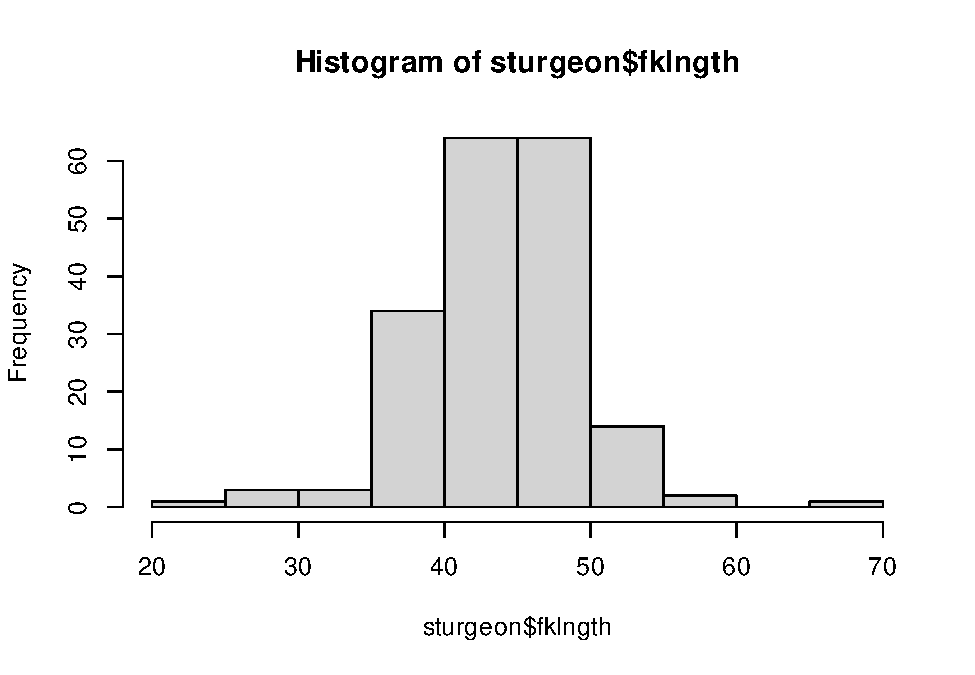
\includegraphics{Labs_BIO4158_files/figure-latex/hist-stur-1.pdf}
\caption{\label{fig:hist-stur}Histogram of fluke length of sturgeons}
\end{figure}

The data appear to be approximately normal. This is good to know.

\begin{rmdnote}
Note that this syntax is a bit heavy as you need to prefix variable names by the data frame name \texttt{sturgeon\$}. You can lighten the syntax by making the variables directly accessible by commands by typing the command \texttt{attach()}.
However, I \textbf{strongly recommend not to use} it because it can lead to many problems hard to detect compare to the little benfit is provides
\end{rmdnote}

This histogram (Fig. \ref{fig:hist-stur}) is a very classical representation of the distribution. Histograms are not perfect however because their shape partly depends on the number of bins used, more so for small samples. One can do better, especially if you want to visually compare the observed distribution to a normal distribution. But you need to come up with a bit of extra R code based on the \texttt{ggplot2} 📦.

\begin{Shaded}
\begin{Highlighting}[]
\CommentTok{\#\# load ggplot2 if needed}
\KeywordTok{library}\NormalTok{(ggplot2)}

\CommentTok{\#\# use "sturgeon" dataframe to make plot called mygraph}
\CommentTok{\# and define x axis as representing fklngth}
\NormalTok{mygraph \textless{}{-}}\StringTok{ }\KeywordTok{ggplot}\NormalTok{(}\DataTypeTok{data =}\NormalTok{ sturgeon, }\KeywordTok{aes}\NormalTok{(}\DataTypeTok{x =}\NormalTok{ fklngth))}

\CommentTok{\#\# add data to the mygraph ggplot}
\NormalTok{mygraph \textless{}{-}}\StringTok{ }\NormalTok{mygraph }\OperatorTok{+}
\StringTok{  }\CommentTok{\#\# add semitransparent histogram}
\StringTok{  }\KeywordTok{geom\_histogram}\NormalTok{(}\KeywordTok{aes}\NormalTok{(}\DataTypeTok{y =}\NormalTok{ ..density..),}
    \DataTypeTok{bins =} \DecValTok{30}\NormalTok{, }\DataTypeTok{color =} \StringTok{"black"}\NormalTok{, }\DataTypeTok{alpha =} \FloatTok{0.3}
\NormalTok{  ) }\OperatorTok{+}
\StringTok{  }\CommentTok{\#\#  add density smooth}
\StringTok{  }\KeywordTok{geom\_density}\NormalTok{() }\OperatorTok{+}
\StringTok{  }\CommentTok{\#\# add observations positions or rug bars}
\StringTok{  }\KeywordTok{geom\_rug}\NormalTok{() }\OperatorTok{+}
\StringTok{  }\CommentTok{\#\# add Gaussian curve adjusted to the data with mean and sd from fklngth}
\StringTok{  }\KeywordTok{stat\_function}\NormalTok{(}
    \DataTypeTok{fun =}\NormalTok{ dnorm,}
    \DataTypeTok{args =} \KeywordTok{list}\NormalTok{(}
      \DataTypeTok{mean =} \KeywordTok{mean}\NormalTok{(sturgeon}\OperatorTok{$}\NormalTok{fklngth),}
      \DataTypeTok{sd =} \KeywordTok{sd}\NormalTok{(sturgeon}\OperatorTok{$}\NormalTok{fklngth)}
\NormalTok{    ),}
    \DataTypeTok{color =} \StringTok{"red"}
\NormalTok{  )}

\CommentTok{\#\# display graph}
\NormalTok{mygraph}
\end{Highlighting}
\end{Shaded}

\begin{figure}
\centering
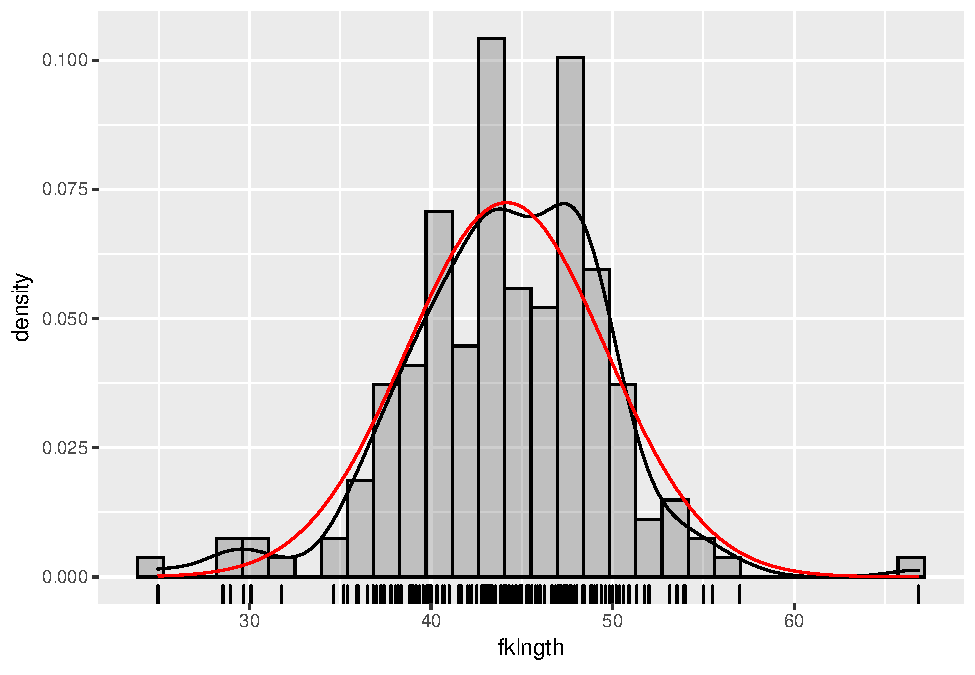
\includegraphics{Labs_BIO4158_files/figure-latex/stur-g1-1.pdf}
\caption{\label{fig:stur-g1}Distribution of fluke length in sturgeon plotted with ggplot}
\end{figure}

Each observation is represented by a short vertical bar below the x- axis (rug). The red line is the normal distribution with the same mean and standard deviation as the data. The other line is the empirical distribution, smoothed from the observations.

The ggplot object you just created (\texttt{mygraph}) can be further manipulated. For example, you can plot the distribution of \texttt{fklngth} per \texttt{sex} and \texttt{year} groups simply by adding a \texttt{facet\_grid()} statement:

\begin{Shaded}
\begin{Highlighting}[]
\NormalTok{mygraph }\OperatorTok{+}\StringTok{ }\KeywordTok{facet\_grid}\NormalTok{(year }\OperatorTok{\textasciitilde{}}\StringTok{ }\NormalTok{sex)}
\end{Highlighting}
\end{Shaded}

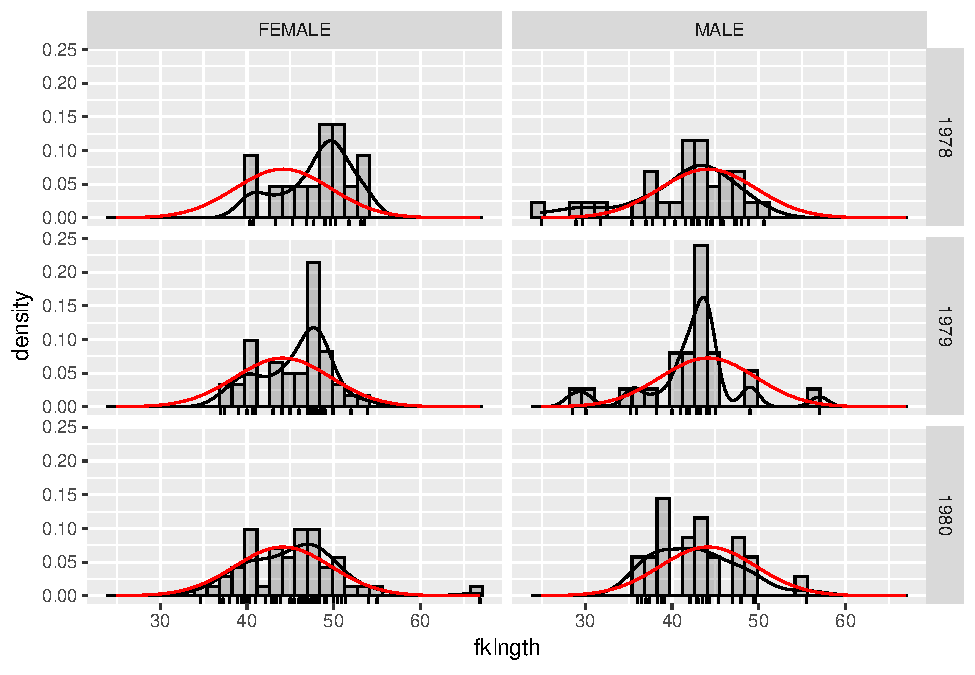
\includegraphics{Labs_BIO4158_files/figure-latex/aventure-1.pdf}

Each panel contains the data distribution for one sex that year, and the recurring red curve is the normal distribution for the entire data set. It can serve as a reference to help visually evaluate differences among panels.

Another way to visually assess normality of data is the QQ plot that is
obtained by the pair of commands \texttt{qqnorm()} and \texttt{qqline()}.

\begin{Shaded}
\begin{Highlighting}[]
\KeywordTok{qqnorm}\NormalTok{(sturgeon}\OperatorTok{$}\NormalTok{fklngth)}
\KeywordTok{qqline}\NormalTok{(sturgeon}\OperatorTok{$}\NormalTok{fklngth)}
\end{Highlighting}
\end{Shaded}

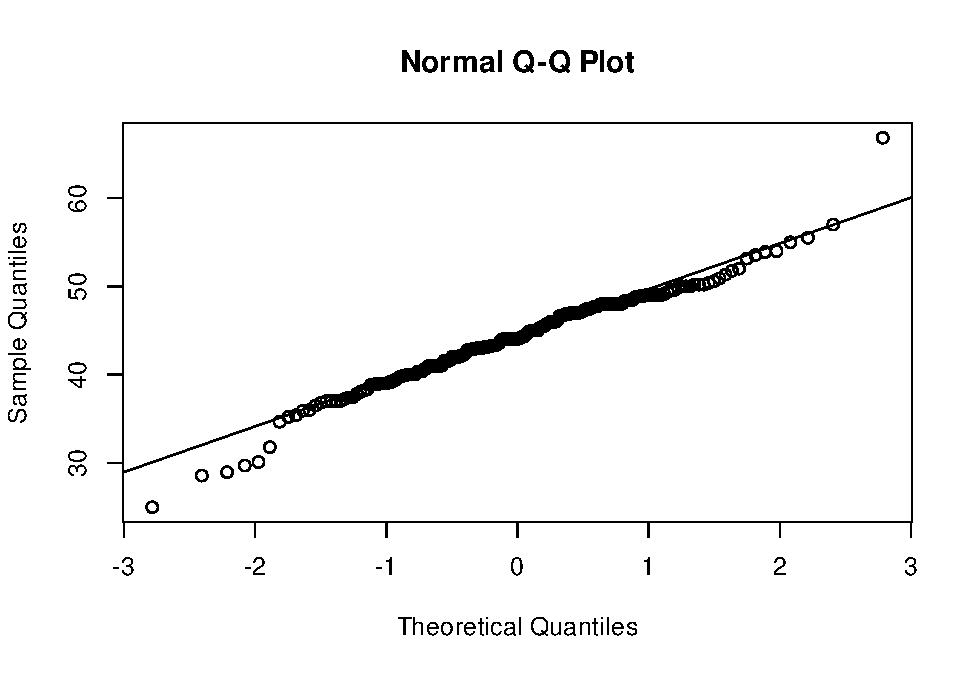
\includegraphics{Labs_BIO4158_files/figure-latex/stur-norm-1.pdf}
Perfectly normal data would follow the straight diagonal line. Here there are deviations in the tails of the distribution and a bit to the right of the center.
Compare this representation to the two preceding graphs.
You will probably agree that it is easier to visualize how data deviate from normality by looking at a histogram of an empirical probability density than by looking at the QQ plots.
However, QQ plots are often automatically produced by various statistical routines and you should be able to interpret them.
In addition, one can easily run a formal test of normality in R with the command \texttt{shapiro.test()} that computes a statistic (\texttt{W}) that measures how tightly data fall around the straight diagonal line of the QQ plot. If data fall perfectly on the line, then \texttt{W\ =\ 1}. If \texttt{W} is much less than 1, then data are not normal.

For the \texttt{fklngth} data:

\begin{Shaded}
\begin{Highlighting}[]
\KeywordTok{shapiro.test}\NormalTok{(sturgeon}\OperatorTok{$}\NormalTok{fklngth)}
\end{Highlighting}
\end{Shaded}

\begin{verbatim}
## 
##  Shapiro-Wilk normality test
## 
## data:  sturgeon$fklngth
## W = 0.97225, p-value = 0.0009285
\end{verbatim}

W is close to 1, but far enough to indicate a statistically significant deviation from normality.

Visual examination of very large data sets is often made difficult by the superposition of data points. Boxplots are an interesting alternative.
The command \texttt{boxplot(fklngth\textasciitilde{}sex,\ notch=TRUE)} produces a boxplot of \texttt{fklngth} for each \texttt{sex} , and adds whiskers.

\begin{Shaded}
\begin{Highlighting}[]
\KeywordTok{boxplot}\NormalTok{(fklngth }\OperatorTok{\textasciitilde{}}\StringTok{ }\NormalTok{sex, }\DataTypeTok{data =}\NormalTok{ sturgeon, }\DataTypeTok{notch =} \OtherTok{TRUE}\NormalTok{)}
\end{Highlighting}
\end{Shaded}

\begin{figure}
\centering
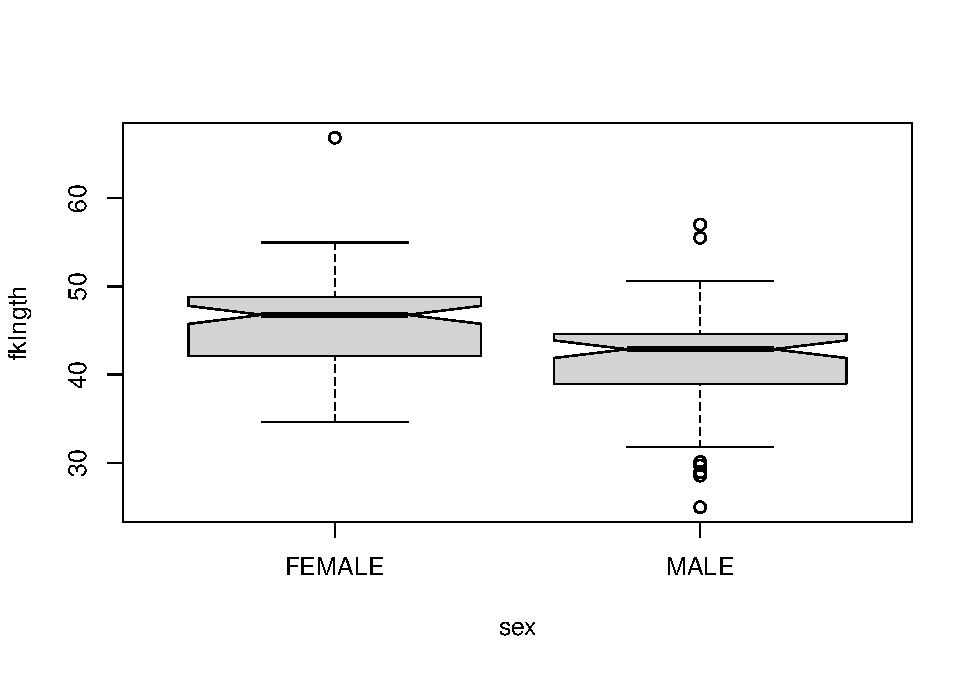
\includegraphics{Labs_BIO4158_files/figure-latex/boxplot-stur-1.pdf}
\caption{\label{fig:boxplot-stur}Boxplot of fluke length in strugeon by sex}
\end{figure}

The slightly thicker line inside the box of figure \ref{fig:boxplot-stur} indicates the median.
The width of the notch is proportional to the uncertainty around the median estimate.
One can visually assess the approximate statistical significance of differences among medians by looking at the overlap of the notches (here there is no overlap and one could tentatively conclude that the median female size is larger than the median male size).
Boxes extend from the first to third quartile (the 25\textsuperscript{th} to 75\textsuperscript{th} percentile if you prefer).
Bars (whiskers) extend above and below the boxes from the minimum to the maximum observed value or, if there are extreme values, from the smallest to the largest observed value within 1.5x the interquartile range from the median. Observations exceeding the limits of the whiskers (hence further away from the median than 1.5x the interquartile range, the range between the 25\textsuperscript{th} and 75\textsuperscript{th} percentile) are plotted as circles. These are outliers, possibly aberrant data.

\hypertarget{scatterplots}{%
\subsection{Scatterplots}\label{scatterplots}}

In addition to histograms and other univariate plots, it is often informative to examine scatter plots.
The command \texttt{plot(y\textasciitilde{}x)} produces a scatter plot of y on the vertical axis (the ordinate) vs x on the horizontal axis (abscissa).

\begin{rmdcode}
Create a scatterplot of fklngth vs age using the plot() command.
\end{rmdcode}

You should obtain:

\begin{Shaded}
\begin{Highlighting}[]
\KeywordTok{plot}\NormalTok{(fklngth }\OperatorTok{\textasciitilde{}}\StringTok{ }\NormalTok{age, }\DataTypeTok{data =}\NormalTok{ sturgeon)}
\end{Highlighting}
\end{Shaded}

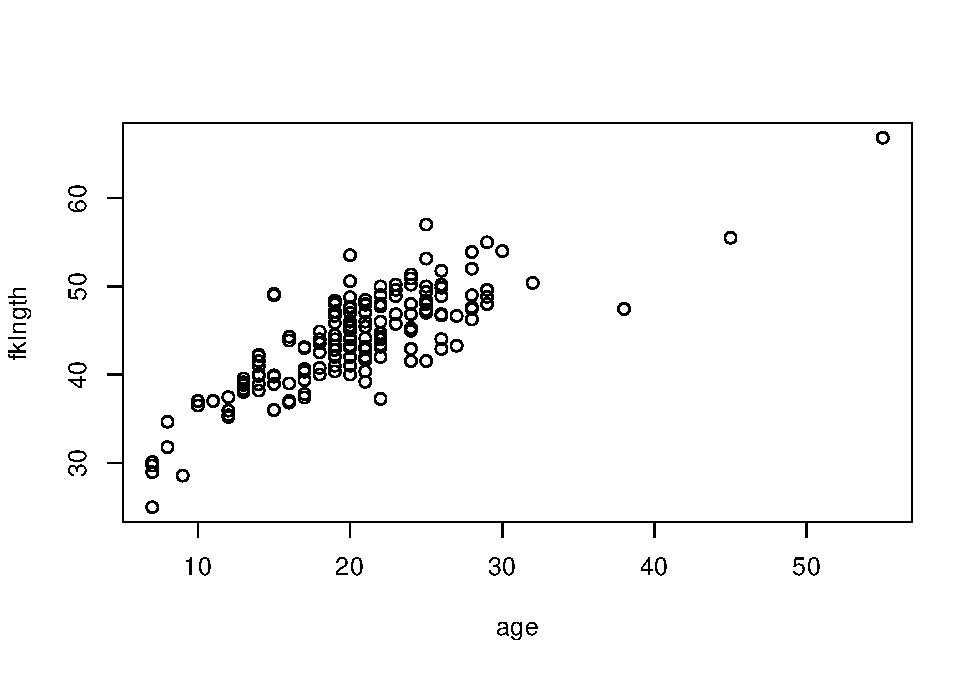
\includegraphics{Labs_BIO4158_files/figure-latex/stur-biv-plot-1.pdf}

R has a function to create all pairwise scatterplots rapidly called
\texttt{pairs()} . One of \texttt{pairs()} options is the addition of a lowess trace on
each plot to that is a smoothed trend in the data.
To get the plot matrix with the lowess smooth for all variables in the
sturgeon data frame, execute the command
\texttt{pairs(sturgeon,\ panel=panel.smooth)}. Howeber given the large number of variable in \texttt{sturgeon} we can limit the plot to the first 6 columns in the data.

\begin{Shaded}
\begin{Highlighting}[]
\KeywordTok{pairs}\NormalTok{(sturgeon[, }\DecValTok{1}\OperatorTok{:}\DecValTok{6}\NormalTok{], }\DataTypeTok{panel =}\NormalTok{ panel.smooth)}
\end{Highlighting}
\end{Shaded}

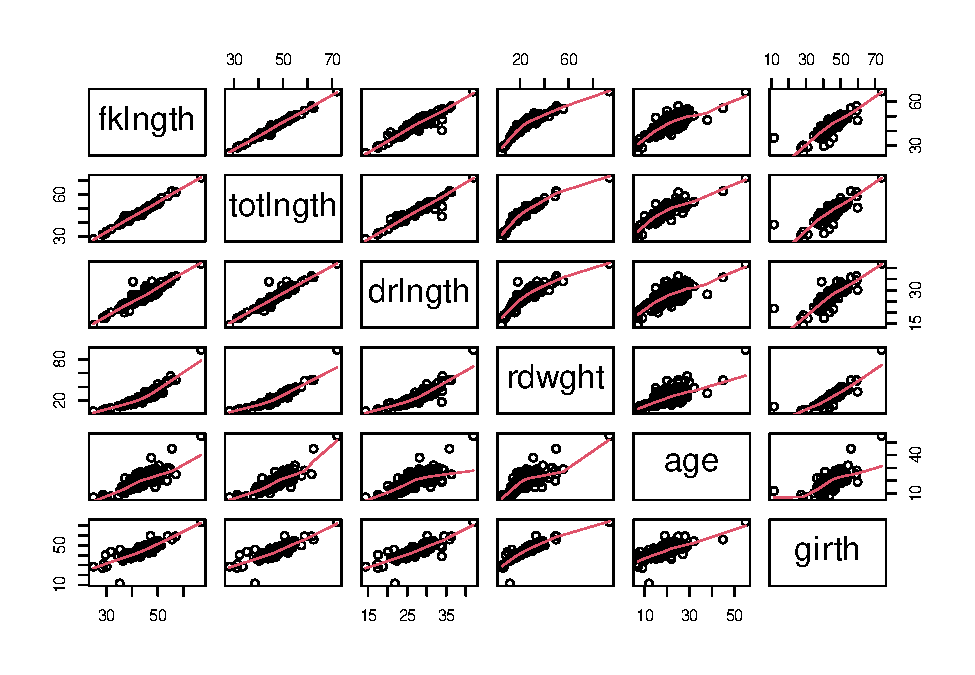
\includegraphics{Labs_BIO4158_files/figure-latex/pairs-stur-1.pdf}

\hypertarget{creating-data-subsets}{%
\section{Creating data subsets}\label{creating-data-subsets}}

You will frequently want to do analyses on some subset of your data.
The command \texttt{subset()} is what you need to isolate cases meeting some criteria.
For example, to create a subset of the sturgeon data frame that contains only females caught in 1978, you could write:

\begin{Shaded}
\begin{Highlighting}[]
\NormalTok{sturgeon\_female\_}\DecValTok{1978}\NormalTok{ \textless{}{-}}\StringTok{ }\KeywordTok{subset}\NormalTok{(sturgeon, sex }\OperatorTok{==}\StringTok{ "FEMALE"} \OperatorTok{\&}\StringTok{ }\NormalTok{year }\OperatorTok{==}\StringTok{ "1978"}\NormalTok{)}
\NormalTok{sturgeon\_female\_}\DecValTok{1978}
\end{Highlighting}
\end{Shaded}

\begin{verbatim}
##      fklngth totlngth  drlngth rdwght age girth    sex   location year
## 2   50.19685 54.13386 31.49606     NA  24  53.5 FEMALE    THE_PAS 1978
## 4   50.19685 53.14961 32.28346     NA  23  52.5 FEMALE    THE_PAS 1978
## 6   49.60630 53.93701 31.10236  35.86  23  54.2 FEMALE    THE_PAS 1978
## 7   47.71654 51.37795 33.97638  33.88  20  48.0 FEMALE    THE_PAS 1978
## 15  48.89764 53.93701 29.92126  35.86  23  52.5 FEMALE    THE_PAS 1978
## 105 46.85039       NA 28.34646  23.90  24    NA FEMALE CUMBERLAND 1978
## 106 40.74803       NA 24.80315  17.50  18    NA FEMALE CUMBERLAND 1978
## 107 40.35433       NA 25.59055  20.90  21    NA FEMALE CUMBERLAND 1978
## 109 43.30709       NA 27.95276  24.10  19    NA FEMALE CUMBERLAND 1978
## 113 53.54331       NA 33.85827  48.90  20    NA FEMALE CUMBERLAND 1978
## 114 51.77165       NA 31.49606  35.30  26    NA FEMALE CUMBERLAND 1978
## 116 45.27559       NA 26.57480  23.70  24    NA FEMALE CUMBERLAND 1978
## 118 53.14961       NA 32.67717  45.30  25    NA FEMALE CUMBERLAND 1978
## 119 50.19685       NA 32.08661  33.90  26    NA FEMALE CUMBERLAND 1978
## 123 49.01575       NA 29.13386  37.50  22    NA FEMALE CUMBERLAND 1978
\end{verbatim}

\begin{rmdcaution}
When using criteria to select cases, be careful of the \texttt{==} syntax to mean equal to.
In this context, if you use a single \texttt{=}, you will not get what you want.
The following table lists the most common criteria to create expressions and their R syntax.
\end{rmdcaution}

\begin{longtable}[]{@{}llll@{}}
\toprule
Operator & Explanation & Operator & Explanation\tabularnewline
\midrule
\endhead
== & Equal to & != & Not equal to\tabularnewline
\textgreater{} & Larger than & \textless{} & Lower than\tabularnewline
\textgreater= & Larger than or equal to & \textless= & Lower than or equal to\tabularnewline
\& & And (vectorized) & \textbar{} & Or (vectorized)\tabularnewline
\&\& & And (control) & \textbar\textbar{} & Or (control)\tabularnewline
! & Not & &\tabularnewline
\bottomrule
\end{longtable}

\begin{rmdcode}
Using the commands \texttt{subset()} and \texttt{hist()} , create a histogram for females caught in 1979 and 1980 (hint: \texttt{sex=="FEMALE"\ \&\ (year\ =="1979"\ \textbar{}\ year=="1980")})
\end{rmdcode}

\begin{figure}
\centering
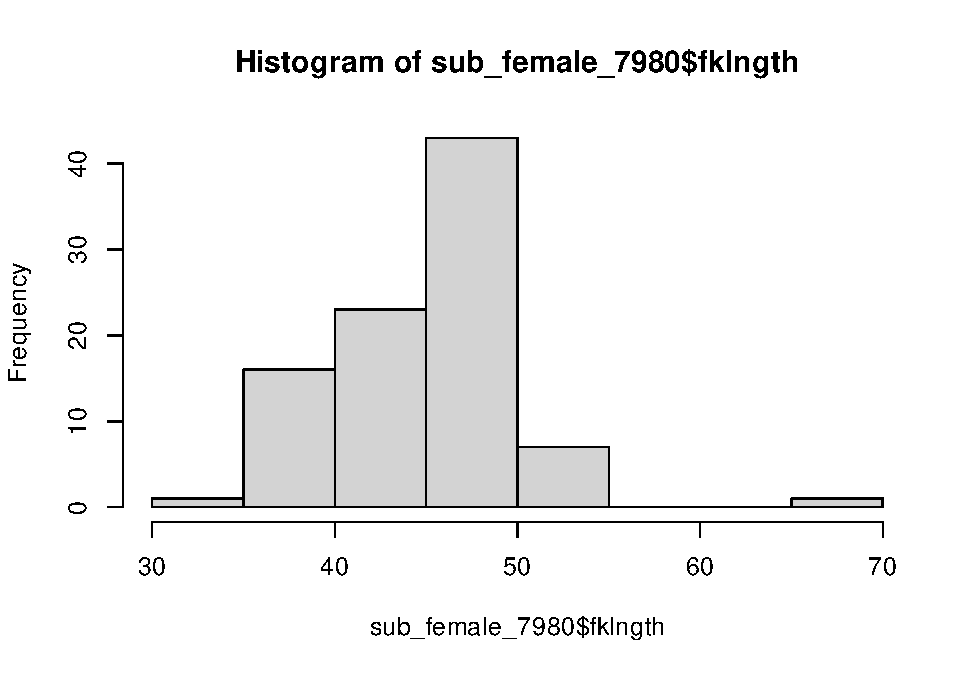
\includegraphics{Labs_BIO4158_files/figure-latex/intror-subex-1.pdf}
\caption{\label{fig:intror-subex}Distibution of fluke length of female sturgeons in 1979 and 1980}
\end{figure}

\hypertarget{data-transformation}{%
\section{Data transformation}\label{data-transformation}}

You will frequently transform raw data to better satisfy assumptions of statistical tests. R will allow you to do that easily.
The most used functions are probably:

\begin{itemize}
\tightlist
\item
  \texttt{log()}
\item
  \texttt{sqrt()}
\item
  \texttt{ifelse()}
\end{itemize}

You can use these functions directly within commands, create vector variables, or add columns in data frames.
To do a plot of the decimal log of fklngth vs age, you can simply use the \texttt{log10()} function within the plot command:

\begin{Shaded}
\begin{Highlighting}[]
\KeywordTok{plot}\NormalTok{(}\KeywordTok{log10}\NormalTok{(fklngth)}\OperatorTok{\textasciitilde{}}\NormalTok{age, }\DataTypeTok{data =}\NormalTok{ sturgeon)}
\end{Highlighting}
\end{Shaded}

To create a vector variable, an orphan variable if you wish, one that is not part of a data frame, called \texttt{lfklngth} and corresponding too the decimal log of \texttt{fklngth}, simply enter:

\begin{Shaded}
\begin{Highlighting}[]
\NormalTok{logfklngth \textless{}{-}}\StringTok{ }\KeywordTok{log10}\NormalTok{(sturgeon}\OperatorTok{$}\NormalTok{fklngth)}
\end{Highlighting}
\end{Shaded}

If you want this new variable to be added to a data frame, then you must prefix the variable name by the data frame name and the \texttt{\$} symbol.
For example to add the variable \texttt{lfkl} containing the decimal log of \texttt{fklngth} to the \texttt{sturgeon} data frame, enter:

\begin{Shaded}
\begin{Highlighting}[]
\NormalTok{sturgeon}\OperatorTok{$}\NormalTok{lfkl \textless{}{-}}\StringTok{ }\KeywordTok{log10}\NormalTok{(sturgeon}\OperatorTok{$}\NormalTok{fklngth)}
\end{Highlighting}
\end{Shaded}

\texttt{lfkl} will be added to the data frame \texttt{sturgeon} for the R session.
Do not forget to save the modified data frame if you want to keep the modified version. Or better, save you Rscript and do not forget to run the line of code again next time you need it.

For conditional transformations, you can use the function \texttt{ifelse()}.
For example, to create a new variable called dummy with a value of 1 for males and 0 for females, you can use:

\begin{Shaded}
\begin{Highlighting}[]
\NormalTok{sturgeon}\OperatorTok{$}\NormalTok{dummy \textless{}{-}}\StringTok{ }\KeywordTok{ifelse}\NormalTok{(sturgeon}\OperatorTok{$}\NormalTok{sex }\OperatorTok{==}\StringTok{ "MALE"}\NormalTok{, }\DecValTok{1}\NormalTok{, }\DecValTok{0}\NormalTok{)}
\end{Highlighting}
\end{Shaded}

\hypertarget{exercice}{%
\section{Exercice}\label{exercice}}

The file \texttt{salmonella.csv} contains numerical values for the variable
called ratio for two environments (\texttt{milieu}: \texttt{IN\ VITRO} or \texttt{IN\ VIVO})
and for 3 strains (\texttt{souche}).
Examine the ratio variable and make a graph to visually assess normality for the wild (SAUVAGE) strain.

\begin{figure}
\centering
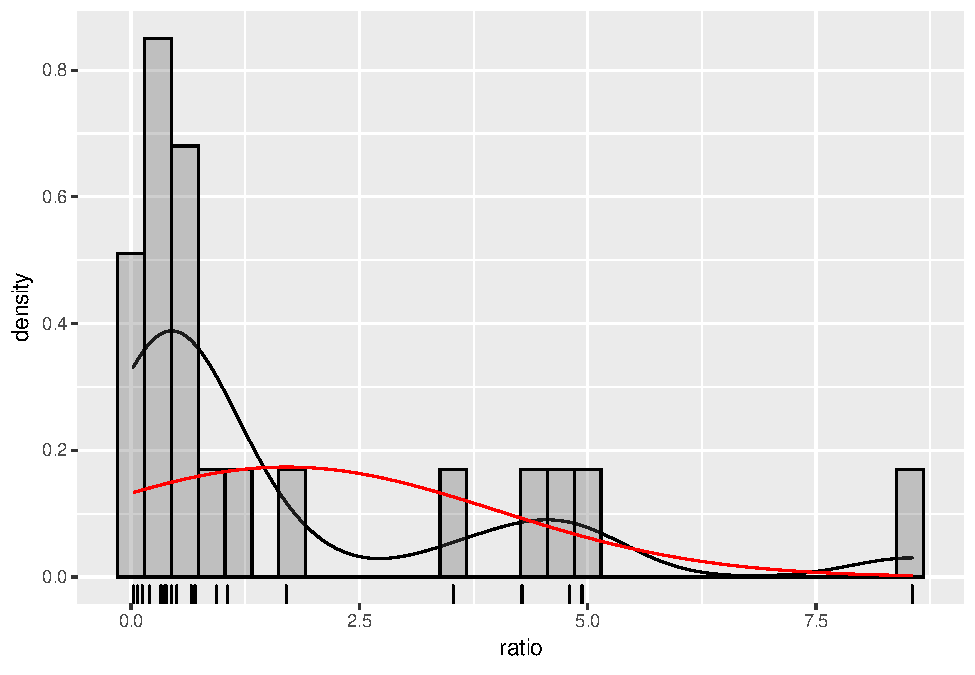
\includegraphics{Labs_BIO4158_files/figure-latex/intror-exer-1.pdf}
\caption{\label{fig:intror-exer}Distibution of infection ratios by the wild (SAUVAGE) strain of salmonella}
\end{figure}

\hypertarget{power-analysis-with-r-and-gpower}{%
\chapter{Power Analysis with R and G*Power}\label{power-analysis-with-r-and-gpower}}

After completing this laboratory, you should :

\begin{itemize}
\tightlist
\item
  be able to compute the power of a t-test with G*Power and R
\item
  be able to calculate the required sample size to achieve a desired power level with a t-test
\item
  be able to calculate the detectable effect size by a t-test given the sample size, the power and \(\alpha\)
\item
  understand how power changes when sample size increases, the effect size changes, or when \(\alpha\) decreases
\item
  understand how power is affected when you change from a two-tailed to a one-tailed test.
\end{itemize}

\hypertarget{the-theory}{%
\section{The theory}\label{the-theory}}

\hypertarget{what-is-power}{%
\subsection{What is power?}\label{what-is-power}}

\emph{Power is the probability of rejecting the null hypothesis when it is false}

\hypertarget{why-do-a-power-analysis}{%
\subsection{Why do a power analysis?}\label{why-do-a-power-analysis}}

\hypertarget{assess-the-strength-of-evidence}{%
\subsubsection*{Assess the strength of evidence}\label{assess-the-strength-of-evidence}}
\addcontentsline{toc}{subsubsection}{Assess the strength of evidence}

Power analysis, performed after accepting a null hypothesis, can help assess the probability of rejecting the null if it were false, and if the magnitude of the effect was equal to that observed (or to any other given magnitude). This type of \emph{a posteriori} analysis is very common.

\hypertarget{design-better-experiments}{%
\subsubsection*{Design better experiments}\label{design-better-experiments}}
\addcontentsline{toc}{subsubsection}{Design better experiments}

Power analysis, performed prior to conducting an experiment (but most often after a preliminary experiment), can be used to determine the number of observations required to detect an effect of a given magnitude with some probability (the power). This type of \emph{a priori} experiment should be more common.

\hypertarget{estimate-minimum-detectable-effect}{%
\subsubsection*{Estimate minimum detectable effect}\label{estimate-minimum-detectable-effect}}
\addcontentsline{toc}{subsubsection}{Estimate minimum detectable effect}

Sampling effort is often predetermined (when you are handed data of an experiment already completed), or extremely constrained (when logistics dictates what can be done). Whether it is \emph{a priori} or \emph{a posteriori}, power analysis can help you estimate, for a fixed sample size and a given power, what is the minimum effect size that can be detected.

\hypertarget{factors-affecting-power}{%
\subsection{Factors affecting power}\label{factors-affecting-power}}

For a given statistical test, there are 3 factors that affect power.

\hypertarget{decision-criteria}{%
\subsubsection*{Decision criteria}\label{decision-criteria}}
\addcontentsline{toc}{subsubsection}{Decision criteria}

Power is related to \(\alpha\), the probability level at which one rejects the null hypothesis. If this decision criteria is made very strict (i.e.~if critical \(\alpha\) is set to a very low value, like 0.1\% or \(p = 0.001\)), then power will be lower than if the critical \(\alpha\) was less strict.

\hypertarget{sample-size}{%
\subsubsection*{Sample size}\label{sample-size}}
\addcontentsline{toc}{subsubsection}{Sample size}

The larger the sample size, the larger the power. As sample size increases, one's ability to detect small effect sizes as being statistically significant gets better.

\hypertarget{effect-size}{%
\subsubsection*{Effect size}\label{effect-size}}
\addcontentsline{toc}{subsubsection}{Effect size}

The larger the effect size, the larger the power. For a given sample size, the ability to detect an effect as being significant is higher for large effects than for small ones. Effect size measures how false the null hypothesis is.

\hypertarget{what-is-gpower}{%
\section{What is G*Power?}\label{what-is-gpower}}

G*Power is free software developed by quantitative psychologists from the University of Dusseldorf in Germany.
It is available in MacOS and Windows versions.
It can be run under Linux using Wine or a virtual machine.

G*Power will allow you to do power analyses for the majority of statistical tests we will cover during the term without making lengthy calculations and looking up long tables and figures of power curves. It is a really useful tool that you need to master.

It is possible to perform all analysis made by G*Power in R, but it requires a bit more code, and a better understanding of the process since everything should be coded by hand. In simple cases, R code is also provided.

\begin{rmdcode}
Download the software \textbf{\href{https://www.psychologie.hhu.de/arbeitsgruppen/allgemeine-psychologie-und-arbeitspsychologie/gpower.html}{here}} and install it on your computer and your workstation (if it is not there already).
\end{rmdcode}

\hypertarget{how-to-use-gpower}{%
\section{How to use G*Power}\label{how-to-use-gpower}}

\hypertarget{general-principle}{%
\subsection{General Principle}\label{general-principle}}

Using G*Power generally involves 3 steps:

\begin{enumerate}
\def\labelenumi{\arabic{enumi}.}
\tightlist
\item
  Choosing the appropriate test
\item
  Choosing one of the 5 types of available power analyses
\item
  Enter parameter values and press the \textbf{Calculate} button
\end{enumerate}

\hypertarget{types-of-power-analyses}{%
\subsection{Types of power analyses}\label{types-of-power-analyses}}

First, \(\alpha\) is define as the probability level at which
one rejects the null hypothesis, and \(\beta\) is \(1 - power\).

\hypertarget{a-priori}{%
\subsubsection*{A priori}\label{a-priori}}
\addcontentsline{toc}{subsubsection}{A priori}

Computes the sample size required given \(\beta\), \(\alpha\), and the effect size. This type of analysis is useful when planning experiments.

\hypertarget{compromise}{%
\subsubsection*{Compromise}\label{compromise}}
\addcontentsline{toc}{subsubsection}{Compromise}

Computes \(\alpha\) and \(\beta\) for a given \(\alpha\)/\(\beta\) ratio, sample size, and effect size. Less commonly used (I have never used it myself) although it can be useful when the \(\alpha\)/\(\beta\) ratio has meaning, for example when the cost of type I and type II errors can be quantified.

\hypertarget{criterion}{%
\subsubsection*{Criterion}\label{criterion}}
\addcontentsline{toc}{subsubsection}{Criterion}

Computes \(\alpha\) for a given \(\beta\), sample size, and effect size. In practice, I see little interest in this. Let me know if you see something I don't!

\hypertarget{post-hoc}{%
\subsubsection*{Post-hoc}\label{post-hoc}}
\addcontentsline{toc}{subsubsection}{Post-hoc}

Computes the power for a given \(\alpha\), effect size, and
sample size. Used frequently to help in the interpretation of a test
that is not statistically significant, but only if an effect size that is
biologically significant is used (and not the observed effect size). Not
relevant when the test is significant.
Sensitivity. Computes the detectable effect size for a given \(\beta\) ,\(\alpha\), and
sample size. Very useful at the planning stage of an experiment.

\hypertarget{how-to-calculate-effect-size}{%
\subsection{How to calculate effect size}\label{how-to-calculate-effect-size}}

G*Power can perform power analyses for several statistical tests.
The metric for effect size depends on the test. Note that other
software packages often use different effect size metrics and that it is
important to use the correct one for each package. G\emph{Power has an
effect size calculator for many tests that only requires you to enter
the relevant values. The following table lists the effect size metrics
used by G}Power for the various tests.

\begin{longtable}[]{@{}lcl@{}}
\toprule
\begin{minipage}[b]{0.11\columnwidth}\raggedright
Test\strut
\end{minipage} & \begin{minipage}[b]{0.35\columnwidth}\centering
Taille d'effet\strut
\end{minipage} & \begin{minipage}[b]{0.46\columnwidth}\raggedright
Formule\strut
\end{minipage}\tabularnewline
\midrule
\endhead
\begin{minipage}[t]{0.11\columnwidth}\raggedright
t-test on means\strut
\end{minipage} & \begin{minipage}[t]{0.35\columnwidth}\centering
d\strut
\end{minipage} & \begin{minipage}[t]{0.46\columnwidth}\raggedright
\(d = \frac{|\mu_1 - \mu_2|}{\sqrt{({s_1}^2 + {s_2}^2)/2}}\)\strut
\end{minipage}\tabularnewline
\begin{minipage}[t]{0.11\columnwidth}\raggedright
t-test on correlations\strut
\end{minipage} & \begin{minipage}[t]{0.35\columnwidth}\centering
r\strut
\end{minipage} & \begin{minipage}[t]{0.46\columnwidth}\raggedright
\strut
\end{minipage}\tabularnewline
\begin{minipage}[t]{0.11\columnwidth}\raggedright
other t-tests\strut
\end{minipage} & \begin{minipage}[t]{0.35\columnwidth}\centering
f\strut
\end{minipage} & \begin{minipage}[t]{0.46\columnwidth}\raggedright
\(f = \frac{\mu_1}{\sigma}\)\strut
\end{minipage}\tabularnewline
\begin{minipage}[t]{0.11\columnwidth}\raggedright
F-test (ANOVA)\strut
\end{minipage} & \begin{minipage}[t]{0.35\columnwidth}\centering
f\strut
\end{minipage} & \begin{minipage}[t]{0.46\columnwidth}\raggedright
\(f = \frac{\frac{\sqrt{\sum_{i=1}^k (\mu_i - \mu)^2}}{k}}{\sigma}\)\strut
\end{minipage}\tabularnewline
\begin{minipage}[t]{0.11\columnwidth}\raggedright
other F-tests\strut
\end{minipage} & \begin{minipage}[t]{0.35\columnwidth}\centering
\(f^2\)\strut
\end{minipage} & \begin{minipage}[t]{0.46\columnwidth}\raggedright
\(f^2 = \frac{{R_p}^2}{1-{R_p}^2}\)\strut
\end{minipage}\tabularnewline
\begin{minipage}[t]{0.11\columnwidth}\raggedright
\strut
\end{minipage} & \begin{minipage}[t]{0.35\columnwidth}\centering
\strut
\end{minipage} & \begin{minipage}[t]{0.46\columnwidth}\raggedright
\({R_p}\) is the squared partial correlation coefficient\strut
\end{minipage}\tabularnewline
\begin{minipage}[t]{0.11\columnwidth}\raggedright
Chi-square test\strut
\end{minipage} & \begin{minipage}[t]{0.35\columnwidth}\centering
w\strut
\end{minipage} & \begin{minipage}[t]{0.46\columnwidth}\raggedright
\(w = \sqrt{ \sum_{i=1}^m \frac{(p_{0i} - p_{1i})^2 }{ p_{0i}} }\)\strut
\end{minipage}\tabularnewline
\begin{minipage}[t]{0.11\columnwidth}\raggedright
\strut
\end{minipage} & \begin{minipage}[t]{0.35\columnwidth}\centering
\strut
\end{minipage} & \begin{minipage}[t]{0.46\columnwidth}\raggedright
\(p_{0i}\) and \(p_{1i}\) are theporportion in category \(i\) predicted by the null, \(_0\), and alternative, \(_1\), hypothesis\strut
\end{minipage}\tabularnewline
\bottomrule
\end{longtable}

\hypertarget{power-analysis-for-a-t-test-on-two-independent-means}{%
\section{Power analysis for a t-test on two independent means}\label{power-analysis-for-a-t-test-on-two-independent-means}}

The objective of this lab is to learn to use G*Power and understand how the 4 parameters of power analyses (\(\alpha\), \(\beta\), sample size and effect size) are related to each other. For this, you will only use the standard t-test to compare two independent means. This is the test most used by biologists, you have all used it, and it will serve admirably for this lab. What you will learn today will be applicable to all other power analyses.

Jaynie Stephenson studied the productivity of streams in the Ottawa region. She has measured fish biomass in 36 streams, 18 on the Shield and 18 in the Ottawa Valley. She found that fish biomass was lower in streams from the valley (2.64 \(g/m^2\) , standard deviation = 3.28) than from the Shield (3.31 \(g/m^2\) , standard deviation = 2.79.).

When she tested the null hypothesis that fish biomass is the same in the two regions by a t-test, she obtained:

\begin{verbatim}
Pooled-Variance Two-Sample t-Test
t = -0.5746, df = 34, p-value = 0.5693
\end{verbatim}

She therefore accepted the null hypothesis (since p is much larger than 0.05) and concluded that fish biomass is the same in the two regions.

\hypertarget{post-hoc-analysis}{%
\subsection{Post-hoc analysis}\label{post-hoc-analysis}}

Using the observed means and standard deviations, we can use G*Power to calculate the power of the two-tailed t-test for two independent means, using the observed effect size (the difference between the two means, weighted by the standard deviations) for \(\alpha\) = 0.05.

Start G*Power.

\begin{enumerate}
\def\labelenumi{\arabic{enumi}.}
\tightlist
\item
  In *\textbf{Test family} , choose: t tests
\item
  For \textbf{Statistical test} , choose: Means: Difference between two independent means (two groups)
\item
  For \textbf{Type of power analysis} , choose: Post hoc: Compute achieved power - given \(\alpha\), sample size, and effect size
\item
  At \textbf{Input Parameters} ,
\end{enumerate}

\begin{itemize}
\tightlist
\item
  in the box \textbf{Tail(s)} , chose: Two,
\item
  check that \(\alpha\) \textbf{err prob} is equal to 0.05
\item
  Enter 18 for the \textbf{Sample size} of group 1 and of group 2
\item
  then, to calculate effect size (d), click on \textbf{Determine =\textgreater{}}
\end{itemize}

\begin{enumerate}
\def\labelenumi{\arabic{enumi}.}
\setcounter{enumi}{4}
\tightlist
\item
  In the window that opens,
\end{enumerate}

\begin{itemize}
\tightlist
\item
  select \textbf{n1 = n2} , then
\item
  enter the two means (\textbf{Mean group} 1 et 2)
\item
  the two standard deviations(\textbf{SD group} 1 et 2)
\item
  click on \textbf{Calculate} and \textbf{transfer to main window}
\end{itemize}

\begin{enumerate}
\def\labelenumi{\arabic{enumi}.}
\setcounter{enumi}{5}
\tightlist
\item
  After you click on the \textbf{Calculate button} in the main window, you
  should get the following:
\end{enumerate}

\begin{figure}
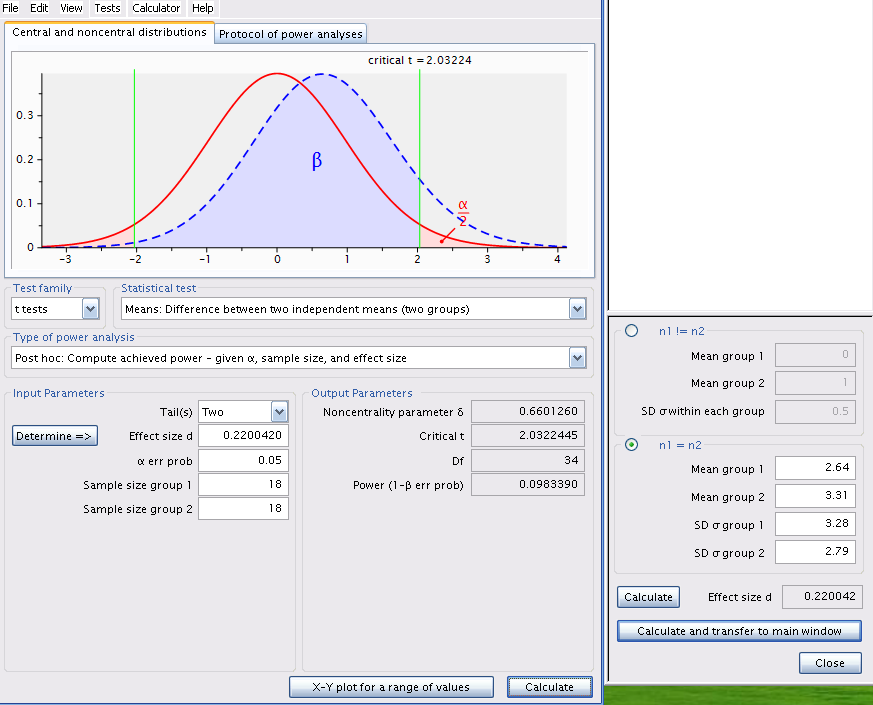
\includegraphics[width=1\linewidth]{images/gpower_1} \caption{Post-hoc analysis with estimated effect size}\label{fig:gpower-1}
\end{figure}

Similar analysis can be done in R. You first need to calculate the effect size \texttt{d} for a t-test comparing 2 means, and then use the \texttt{pwr.t.test()} function from the \texttt{pwr} 📦.
The easiest is to create anew function in R to estimate the effect size \texttt{d}since we are going to reuse it multiple times during the lab.

\begin{Shaded}
\begin{Highlighting}[]
\CommentTok{\# load package pwr}
\KeywordTok{library}\NormalTok{(pwr)}
\CommentTok{\# define d for a 2 sample t{-}test}
\NormalTok{d \textless{}{-}}\StringTok{ }\ControlFlowTok{function}\NormalTok{(u1, u2, sd1, sd2) \{}
  \KeywordTok{abs}\NormalTok{(u1 }\OperatorTok{{-}}\StringTok{ }\NormalTok{u2) }\OperatorTok{/}\StringTok{ }\KeywordTok{sqrt}\NormalTok{((sd1}\OperatorTok{\^{}}\DecValTok{2} \OperatorTok{+}\StringTok{ }\NormalTok{sd2}\OperatorTok{\^{}}\DecValTok{2}\NormalTok{) }\OperatorTok{/}\StringTok{ }\DecValTok{2}\NormalTok{)}
\NormalTok{\}}

\CommentTok{\# power analysis}
\KeywordTok{pwr.t.test}\NormalTok{(}
  \DataTypeTok{n =} \DecValTok{18}\NormalTok{,}
  \DataTypeTok{d =} \KeywordTok{d}\NormalTok{(}\DataTypeTok{u1 =} \FloatTok{2.64}\NormalTok{, }\DataTypeTok{sd1 =} \FloatTok{3.28}\NormalTok{, }\DataTypeTok{u2 =} \FloatTok{3.31}\NormalTok{, }\DataTypeTok{sd2 =} \FloatTok{2.79}\NormalTok{),}
  \DataTypeTok{sig.level =} \FloatTok{0.05}\NormalTok{,}
  \DataTypeTok{type =} \StringTok{"two.sample"}\NormalTok{)}
\end{Highlighting}
\end{Shaded}

\begin{verbatim}
## 
##      Two-sample t test power calculation 
## 
##               n = 18
##               d = 0.220042
##       sig.level = 0.05
##           power = 0.09833902
##     alternative = two.sided
## 
## NOTE: n is number in *each* group
\end{verbatim}

\begin{Shaded}
\begin{Highlighting}[]
\CommentTok{\# plot similar to G*Power}
\NormalTok{x \textless{}{-}}\StringTok{ }\KeywordTok{seq}\NormalTok{(}\OperatorTok{{-}}\DecValTok{4}\NormalTok{, }\DecValTok{4}\NormalTok{, }\DataTypeTok{length =} \DecValTok{200}\NormalTok{)}
\KeywordTok{plot}\NormalTok{(x, }\KeywordTok{dnorm}\NormalTok{(x), }\DataTypeTok{type =} \StringTok{"l"}\NormalTok{, }\DataTypeTok{col =} \StringTok{"red"}\NormalTok{, }\DataTypeTok{lwd =} \DecValTok{2}\NormalTok{)}
\NormalTok{qc \textless{}{-}}\StringTok{ }\KeywordTok{qt}\NormalTok{(}\FloatTok{0.025}\NormalTok{, }\DecValTok{16}\NormalTok{)}
\KeywordTok{abline}\NormalTok{(}\DataTypeTok{v =}\NormalTok{ qc, }\DataTypeTok{col =} \StringTok{"green"}\NormalTok{)}
\KeywordTok{abline}\NormalTok{(}\DataTypeTok{v =} \OperatorTok{{-}}\NormalTok{qc, }\DataTypeTok{col =} \StringTok{"green"}\NormalTok{)}
\KeywordTok{lines}\NormalTok{(x, }\KeywordTok{dnorm}\NormalTok{(x, }\DataTypeTok{mean =}\NormalTok{ (}\FloatTok{3.31} \OperatorTok{{-}}\StringTok{ }\FloatTok{2.64}\NormalTok{)), }\DataTypeTok{type =} \StringTok{"l"}\NormalTok{, }\DataTypeTok{col =} \StringTok{"blue"}\NormalTok{, }\DataTypeTok{lwd =} \DecValTok{2}\NormalTok{)}

\CommentTok{\# power corresponds to the shaded area}
\NormalTok{y \textless{}{-}}\StringTok{ }\KeywordTok{dnorm}\NormalTok{(x, }\DataTypeTok{mean =}\NormalTok{ (}\FloatTok{3.31} \OperatorTok{{-}}\StringTok{ }\FloatTok{2.64}\NormalTok{))}
\KeywordTok{polygon}\NormalTok{(}
  \KeywordTok{c}\NormalTok{(x[x }\OperatorTok{\textless{}=}\StringTok{ }\OperatorTok{{-}}\NormalTok{qc], }\OperatorTok{{-}}\NormalTok{qc), }\KeywordTok{c}\NormalTok{(y[x }\OperatorTok{\textless{}=}\StringTok{ }\OperatorTok{{-}}\NormalTok{qc], }\DecValTok{0}\NormalTok{),}
  \DataTypeTok{col =} \KeywordTok{rgb}\NormalTok{(}\DataTypeTok{red =} \DecValTok{0}\NormalTok{, }\DataTypeTok{green =} \FloatTok{0.2}\NormalTok{, }\DataTypeTok{blue =} \DecValTok{1}\NormalTok{, }\DataTypeTok{alpha =} \FloatTok{0.5}\NormalTok{))}
\end{Highlighting}
\end{Shaded}

\begin{figure}
\centering
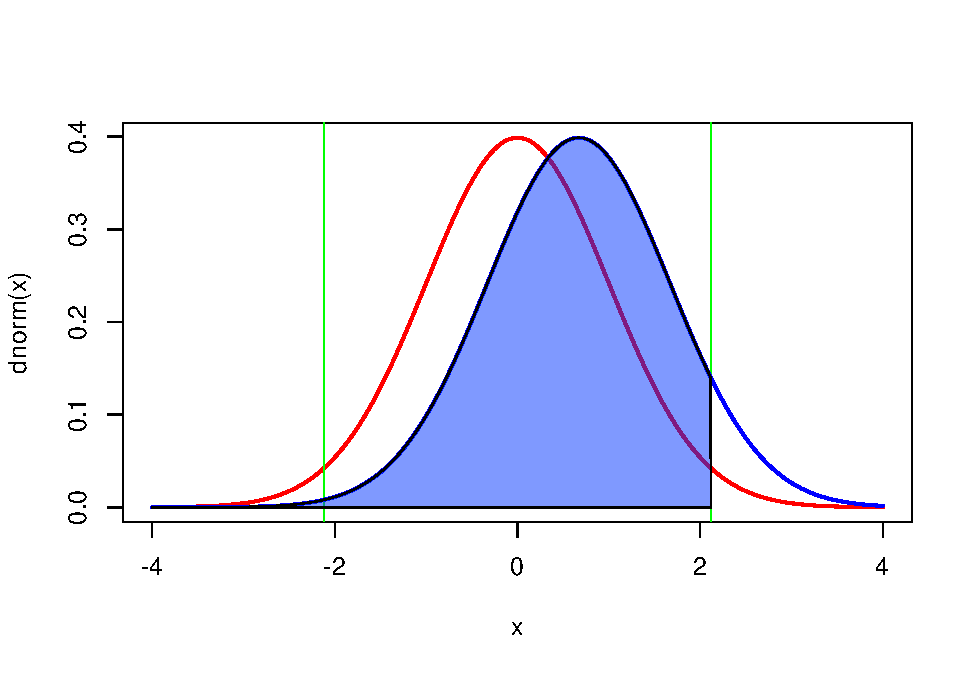
\includegraphics{Labs_BIO4158_files/figure-latex/r-power-1.pdf}
\caption{\label{fig:r-power}Post-hoc analysis with estimated effect size in R}
\end{figure}

Let's examine the figure \ref{fig:gpower-1}.

\begin{itemize}
\tightlist
\item
  The curve on the left, in red, corresponds to the expected distri- bution of the t-statistics when \(H_0\) is true (\emph{i.e.} when the two means are equal) given the sample size (18 per region) and the observed standard deviations.
\item
  The vertical green lines correspond to the critical values of t for \(\alpha = 0.05\) and a total sample size of 36 (2x18).
\item
  The shaded pink regions correspond to the rejection zones for \(H_0\). If Jaynie had obtained a \emph{t-value} outside the interval delimited by the critical values ranging from -2.03224 to 2.03224, she would then have rejected \(H_0\) , the null hypothesis of equal means. In fact, she obtained a t-value of -0.5746 and concluded that the biomass is equal in the two regions.
\item
  The curve on the right, in blue, corresponds to the expected dis- tribution of the t-statistics if \(H_1\) is true (here \(H_1\) is that there is a difference in biomass between the two regions equal to \(3.33 - 2.64 = 0.69 g/m^2\) , given the observed standard deviations). This distribution is what we should observe if \(H_1\) was true and we repeated a large number of times the experiment using random samples of 18 streams in each of the two regions and calculated a t-statistic for each sample. On average, we would obtain a t-statistic of about 0.6.
\item
  Note that there is considerable overlap of the two distributions and that a large fraction of the surface under the right curve is within the interval where \(H_0\) is accepted between the two vertical green lines at -2.03224 and 2.03224. This proportion, shaded in blue under the distribution on the right is labeled \(\beta\) and corresponds to the risk of \emph{type II error} (accept \(H_0\) when \(H_1\) is true).
\item
  Power is simply \(1-\beta\), and is here 0.098339. Therefore, if the mean biomass differed by \(0.69 g/m^2\) between the two regions, Jaynie had only 9.8\% chance of being able to detect it as a statistically significant difference at =5\% with a sample size of 18 streams in each region.
\end{itemize}

\textbf{Let's recapitulate}: The difference in biomass between regions is not statistically significant according to the t-test. It is because the difference is relatively small relative to the precision of the measurements. It is therefore not surprising that that power, i.e.~the probability of detecting a statistically significant difference, is small. Therefore, this analysis is not very informative.

\textbf{Indeed, a post hoc power analysis using the observed effect size is not useful}. It is much more informative to conduct a post hoc power analysis for an effect size that is different from the observed effect size. But what effect size to use? It is the biology of the system under study that will guide you. For example, with respect to fish biomass in streams, one could argue that a two fold change in biomass (say from 2.64 to 5.28 g/m\textsuperscript{2} ) has ecologically significant repercussions. We would therefore want to know if Jaynie had a good chance of detecting a difference as large as this before accepting her conclusion that the biomass is the same in the two regions. So, what were the odds that Jaynie could detect a difference of 2.64 g/m\textsuperscript{2} between the two regions? G*Power can tell you if you cajole it the right way.

\begin{rmdcode}
Change the mean of group 2 to 5.28, recalculate effect size, and click on Calculate to obtain figure \ref{fig:gpower-2}.
\end{rmdcode}

\begin{figure}
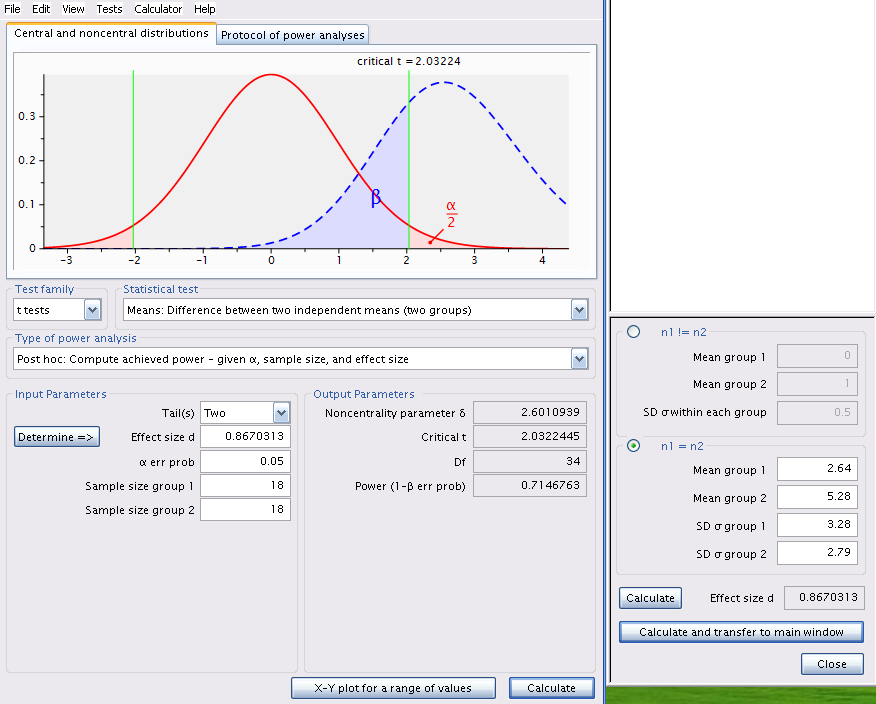
\includegraphics[width=1\linewidth]{images/gpower_2} \caption{Post-hoc analysis using an effect size different from the one estimated}\label{fig:gpower-2}
\end{figure}

Same analysis using R (without all the code for the interesting but not really useful plot)

\begin{Shaded}
\begin{Highlighting}[]
\KeywordTok{pwr.t.test}\NormalTok{(}
  \DataTypeTok{n =} \DecValTok{18}\NormalTok{,}
  \DataTypeTok{d =} \KeywordTok{d}\NormalTok{(}\DataTypeTok{u1 =} \FloatTok{2.64}\NormalTok{, }\DataTypeTok{sd1 =} \FloatTok{3.28}\NormalTok{, }\DataTypeTok{u2 =} \FloatTok{5.28}\NormalTok{, }\DataTypeTok{sd2 =} \FloatTok{2.79}\NormalTok{),}
  \DataTypeTok{sig.level =} \FloatTok{0.05}\NormalTok{,}
  \DataTypeTok{type =} \StringTok{"two.sample"}\NormalTok{)}
\end{Highlighting}
\end{Shaded}

\begin{verbatim}
## 
##      Two-sample t test power calculation 
## 
##               n = 18
##               d = 0.8670313
##       sig.level = 0.05
##           power = 0.7146763
##     alternative = two.sided
## 
## NOTE: n is number in *each* group
\end{verbatim}

The power is 0.71, therefore Jaynie had a reasonable chance (71\%) of detecting a doubling of biomass with 18 streams in each region.

Note that this post hoc power analysis, done for an effect size considered biologically meaningful, is much more informative than the preceeding one done with the observed effect size (which is what too many students do because it is the default of so many power calculation programs). Jaynie did not detect a difference between the two regions. There are two possibilities: 1) there is really no difference between the regions, or 2) the precision of measurements is so low (because the sample size is small and/or there is large variability within a region) that it is very unlikely to be able to detect even large differences. The second power analysis can eliminate this second possibility because Jaynie had 71\% chances of detecting a doubling of biomass.

\hypertarget{a-priori-analysis}{%
\subsection{A priori analysis}\label{a-priori-analysis}}

Suppose that a difference in biomass of \(3.31-2.64 = 0.67 g/m^2\) can be ecologically significant. The next field season should be planned so that Jaynie would have a good chance of detecting such a difference in fish biomass between regions. How many streams should Jaynie sample in each region to have 80\% of detecting such a difference (given the observed variability)?

\begin{rmdcode}
Change the type of power analysis in G*Power to \textbf{A priori: Compute sample size - given \(\alpha\) , power, and effect size}. Ensure that the values for means and standard deviations are those obtained by Jaynie. Recalculate the effect size metric and enter 0.8 for power and you will obtain (\ref{fig:gpower-3}.
\end{rmdcode}

\begin{figure}
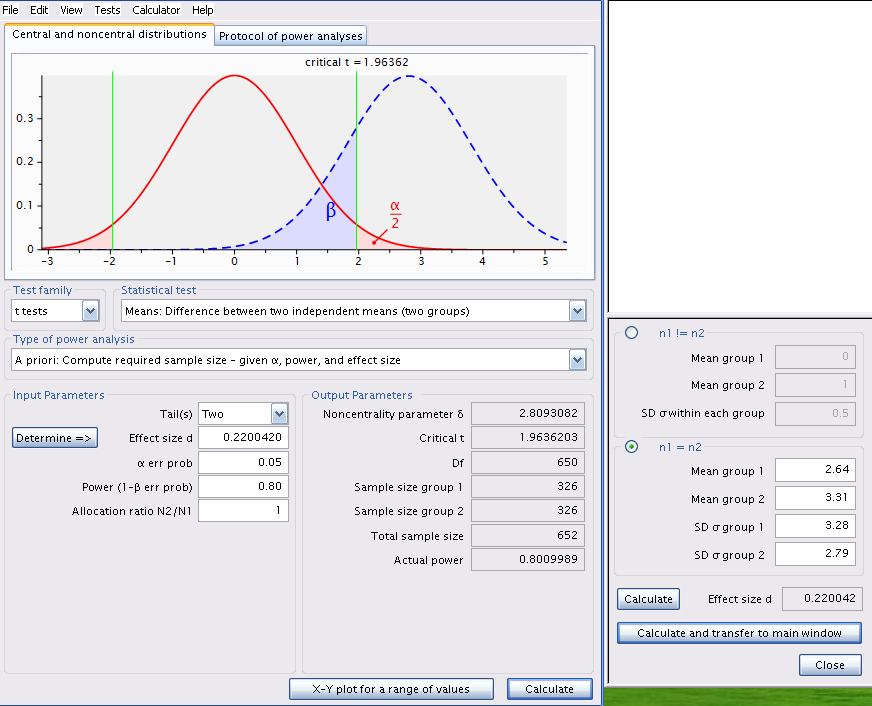
\includegraphics[width=1\linewidth]{images/gpower_3} \caption{A priori analysis}\label{fig:gpower-3}
\end{figure}

\begin{Shaded}
\begin{Highlighting}[]
\KeywordTok{pwr.t.test}\NormalTok{(}
  \DataTypeTok{power =} \FloatTok{0.8}\NormalTok{,}
  \DataTypeTok{d =} \KeywordTok{d}\NormalTok{(}\DataTypeTok{u1 =} \FloatTok{2.64}\NormalTok{, }\DataTypeTok{sd1 =} \FloatTok{3.28}\NormalTok{, }\DataTypeTok{u2 =} \FloatTok{3.31}\NormalTok{, }\DataTypeTok{sd2 =} \FloatTok{2.79}\NormalTok{),}
  \DataTypeTok{sig.level =} \FloatTok{0.05}\NormalTok{,}
  \DataTypeTok{type =} \StringTok{"two.sample"}\NormalTok{)}
\end{Highlighting}
\end{Shaded}

\begin{verbatim}
## 
##      Two-sample t test power calculation 
## 
##               n = 325.1723
##               d = 0.220042
##       sig.level = 0.05
##           power = 0.8
##     alternative = two.sided
## 
## NOTE: n is number in *each* group
\end{verbatim}

\textbf{Ouch!} The required sample would be of 326 streams in each region! It would cost a fortune and require several field teams otherwise only a few dozen streams could be sampled over the summer and it would be very unlikely that such a small difference in biomass could be detected. Sampling fewer streams would probably be in vain and could be considered as a waste of effort and time: why do the work on several dozens of streams if the odds of success are that low?

If we recalculate for a power of 95\%, we find that 538 streams would be required from each region. Increasing power means more work!

\begin{Shaded}
\begin{Highlighting}[]
\KeywordTok{pwr.t.test}\NormalTok{(}
  \DataTypeTok{power =} \FloatTok{0.95}\NormalTok{,}
  \DataTypeTok{d =} \KeywordTok{d}\NormalTok{(}\DataTypeTok{u1 =} \FloatTok{2.64}\NormalTok{, }\DataTypeTok{sd1 =} \FloatTok{3.28}\NormalTok{, }\DataTypeTok{u2 =} \FloatTok{3.31}\NormalTok{, }\DataTypeTok{sd2 =} \FloatTok{2.79}\NormalTok{),}
  \DataTypeTok{sig.level =} \FloatTok{0.05}\NormalTok{,}
  \DataTypeTok{type =} \StringTok{"two.sample"}\NormalTok{)}
\end{Highlighting}
\end{Shaded}

\begin{verbatim}
## 
##      Two-sample t test power calculation 
## 
##               n = 537.7286
##               d = 0.220042
##       sig.level = 0.05
##           power = 0.95
##     alternative = two.sided
## 
## NOTE: n is number in *each* group
\end{verbatim}

\hypertarget{sensitivity-analysis---calculate-the-detectable-effect-size}{%
\subsection{Sensitivity analysis - Calculate the detectable effect size}\label{sensitivity-analysis---calculate-the-detectable-effect-size}}

Given the observed variability, a sampling effort of 18 streams per region, and with \(\alpha\) = 0.05, what effect size could Jaynie detect with 80\% probability \(\beta=0.2\))?

\begin{rmdcode}
Change analysis type in G*Power to \textbf{Sensitivity: Compute required effect size - given \(\alpha\) , power, and sample size} and size is 18 in each region.
\end{rmdcode}

\begin{figure}
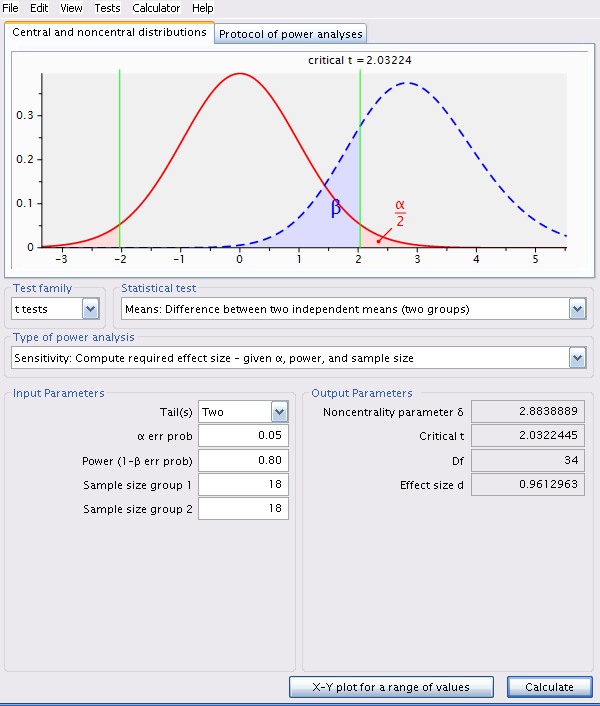
\includegraphics[width=1\linewidth]{images/gpower_4} \caption{Analyse de sensitivité}\label{fig:gpower-4}
\end{figure}

\begin{Shaded}
\begin{Highlighting}[]
\KeywordTok{pwr.t.test}\NormalTok{(}
  \DataTypeTok{power =} \FloatTok{0.8}\NormalTok{,}
  \DataTypeTok{n =} \DecValTok{18}\NormalTok{,}
  \DataTypeTok{sig.level =} \FloatTok{0.05}\NormalTok{,}
  \DataTypeTok{type =} \StringTok{"two.sample"}\NormalTok{)}
\end{Highlighting}
\end{Shaded}

\begin{verbatim}
## 
##      Two-sample t test power calculation 
## 
##               n = 18
##               d = 0.9612854
##       sig.level = 0.05
##           power = 0.8
##     alternative = two.sided
## 
## NOTE: n is number in *each* group
\end{verbatim}

The detectable effect size for this sample size, \(\alpha = 0.05\) and \(\beta = 0.2\) (or power of 80\%) is 0.961296.

\begin{rmdcaution}
Attention, this effect size is the metric \texttt{d} and is dependent on sampling variability.
\end{rmdcaution}

Here, \texttt{d} is approximately equal to

\[ d = \frac{| \bar{X_1} \bar{X_2} |} {\sqrt{\frac{{s_1}^2 +{s_2}^2}{2}}}\]

To convert this d value without units into a value for the detectable difference in biomass between the two regions, you need to multiply \texttt{d} by the denominator of the equation.

\[
| \bar{X_1} - \bar{X_2} | = d * \sqrt{\frac{{s_1}^2 +{s_2}^2}{2}}
\]

In R this can be done with the following code

\begin{Shaded}
\begin{Highlighting}[]
\KeywordTok{pwr.t.test}\NormalTok{(}
  \DataTypeTok{power =} \FloatTok{0.8}\NormalTok{,}
  \DataTypeTok{n =} \DecValTok{18}\NormalTok{,}
  \DataTypeTok{sig.level =} \FloatTok{0.05}\NormalTok{,}
  \DataTypeTok{type =} \StringTok{"two.sample"}\NormalTok{)}\OperatorTok{$}\NormalTok{d }\OperatorTok{*}\StringTok{ }\KeywordTok{sqrt}\NormalTok{((}\FloatTok{3.28}\OperatorTok{\^{}}\DecValTok{2} \OperatorTok{+}\StringTok{ }\FloatTok{2.79}\OperatorTok{\^{}}\DecValTok{2}\NormalTok{) }\OperatorTok{/}\StringTok{ }\DecValTok{2}\NormalTok{)}
\end{Highlighting}
\end{Shaded}

\begin{verbatim}
## [1] 2.926992
\end{verbatim}

Therefore, with 18 streams per region, \(\alpha\) = 0.05 and \(\beta\) = 0.2 (so power of 80\%), Jaynie could detect a difference of 2.93 g/m\textsuperscript{2} between regions, a bit more than a doubling of biomass.

\hypertarget{important-points-to-remember}{%
\section{Important points to remember}\label{important-points-to-remember}}

\begin{itemize}
\tightlist
\item
  Post hoc power analyses are relevant only when the null hypothesis is accepted because it is impossible to make a \emph{type II error} when rejecting \(H_0\) .
\item
  With very large samples, power is very high and minute differences can be statistically detected, even if they are not biologically significant.
\item
  When using a stricter significance criteria (\(\alpha < 0.05\)) power is reduced.
\item
  Maximizing power implies more sampling effort, unless you use a more liberal statistical criteria (\(\alpha > 0.05\))
\item
  The choice of \(\beta\) is somewhat arbitrary. \(\beta=0.2\) (power of 80\%) is considered relatively high by most.
\end{itemize}

\hypertarget{correlation-and-simple-linear-regression}{%
\chapter{Correlation and simple linear regression}\label{correlation-and-simple-linear-regression}}

After completing this laboratory exercise, you should be able to:

\begin{itemize}
\tightlist
\item
  Use R to produce a scatter plot of the relationship between two
  variables.
\item
  Use R to carry out some simple data transformations.
\item
  Use R to compute the Pearson product-moment correlation
  between two variables and assess its statistical significance.
\item
  Use R to compute the correlation between pairs of ranked vari-
  ables using the Spearman rank correlation and Kendall's tau.
\item
  Use R to assess the significance of pairwise comparisons from a
  generalized correlation matrix using Bonferroni-adjusted proba-
  bilities.
\item
  Use R do a simple linear regression
\item
  Use R to test the validity of the assumptions underlying simple lin-
  ear regression
\item
  Use R to assess significance of a regression by the bootstrap
  method
\item
  Quantify effect size in simple regression and perform a power
  analysis using G*Power
\end{itemize}

\hypertarget{set-lm}{%
\section{R packages and data}\label{set-lm}}

For this la b you need:

\begin{itemize}
\tightlist
\item
  R packages:

  \begin{itemize}
  \tightlist
  \item
    car
  \item
    lmtest
  \item
    boot
  \item
    pwr
  \item
    ggplot
  \item
    performance
  \end{itemize}
\item
  data:

  \begin{itemize}
  \tightlist
  \item
    sturgeon.csv
  \end{itemize}
\end{itemize}

You need to load the packages in R with \texttt{library()} and if need needed install them first with \texttt{install.packages()}
For the data, load them using the \texttt{read.csv()} function.

\begin{Shaded}
\begin{Highlighting}[]
\KeywordTok{library}\NormalTok{(car)}
\KeywordTok{library}\NormalTok{(lmtest)}
\KeywordTok{library}\NormalTok{(performance)}
\KeywordTok{library}\NormalTok{(boot)}
\KeywordTok{library}\NormalTok{(ggplot2)}
\KeywordTok{library}\NormalTok{(pwr)}

\NormalTok{sturgeon \textless{}{-}}\StringTok{ }\KeywordTok{read.csv}\NormalTok{(}\StringTok{"data/sturgeon.csv"}\NormalTok{)}
\end{Highlighting}
\end{Shaded}

\begin{rmdnote}
Note that the command to read the data assumes that the data file is in a folder named \texttt{data} within the working directory. Adjust as needed.
\end{rmdnote}

\hypertarget{scatter-plots}{%
\section{Scatter plots}\label{scatter-plots}}

Correlation and regression analysis should always begin with an examination of the data: this is a critical first step in determining whether such analyses are even appropriate for your data.
Suppose we are interested in the extent to which length of male sturgeon in the vicinity of The Pas and Cumberland House covaries with weight. To address this question, we look at the correlation between \texttt{fklngth} and \texttt{rdwght}.
Recall that one of the assumptions in correlation analysis is that the
relationship between the two variables is linear. To evaluate this
assumption, a good first step is to produce a scatterplot.

\begin{itemize}
\tightlist
\item
  Load the data from \texttt{sturgeon.csv} in an obk=jcet named \texttt{sturgeon}.
  Make a scatter plot of \texttt{rdwght} vs \texttt{fklngth} fit with a locally weighted regression (Loess) smoother, and a linear regression line.
\end{itemize}

\begin{Shaded}
\begin{Highlighting}[]
\NormalTok{sturgeon \textless{}{-}}\StringTok{ }\KeywordTok{read.csv}\NormalTok{(}\StringTok{"data/sturgeon.csv"}\NormalTok{)}
\KeywordTok{str}\NormalTok{(sturgeon)}
\end{Highlighting}
\end{Shaded}

\begin{verbatim}
## 'data.frame':    186 obs. of  9 variables:
##  $ fklngth : num  37 50.2 28.9 50.2 45.6 ...
##  $ totlngth: num  40.7 54.1 31.3 53.1 49.5 ...
##  $ drlngth : num  23.6 31.5 17.3 32.3 32.1 ...
##  $ rdwght  : num  15.95 NA 6.49 NA 29.92 ...
##  $ age     : int  11 24 7 23 20 23 20 7 23 19 ...
##  $ girth   : num  40.5 53.5 31 52.5 50 54.2 48 28.5 44 39 ...
##  $ sex     : chr  "MALE" "FEMALE" "MALE" "FEMALE" ...
##  $ location: chr  "THE_PAS" "THE_PAS" "THE_PAS" "THE_PAS" ...
##  $ year    : int  1978 1978 1978 1978 1978 1978 1978 1978 1978 1978 ...
\end{verbatim}

\begin{Shaded}
\begin{Highlighting}[]
\NormalTok{mygraph \textless{}{-}}\StringTok{ }\KeywordTok{ggplot}\NormalTok{(}
  \DataTypeTok{data =}\NormalTok{ sturgeon[}\OperatorTok{!}\KeywordTok{is.na}\NormalTok{(sturgeon}\OperatorTok{$}\NormalTok{rdwght), ], }\CommentTok{\# source of data}
  \KeywordTok{aes}\NormalTok{(}\DataTypeTok{x =}\NormalTok{ fklngth, }\DataTypeTok{y =}\NormalTok{ rdwght)}
\NormalTok{)}
\CommentTok{\# plot data points, regression, loess trace}
\NormalTok{mygraph \textless{}{-}}\StringTok{ }\NormalTok{mygraph }\OperatorTok{+}
\StringTok{  }\KeywordTok{stat\_smooth}\NormalTok{(}\DataTypeTok{method =}\NormalTok{ lm, }\DataTypeTok{se =} \OtherTok{FALSE}\NormalTok{, }\DataTypeTok{color =} \StringTok{"green"}\NormalTok{) }\OperatorTok{+}\StringTok{ }\CommentTok{\# add linear regression, but no SE shading}
\StringTok{  }\KeywordTok{stat\_smooth}\NormalTok{(}\DataTypeTok{color =} \StringTok{"red"}\NormalTok{, }\DataTypeTok{se =} \OtherTok{FALSE}\NormalTok{) }\OperatorTok{+}\StringTok{ }\CommentTok{\# add loess}
\StringTok{  }\KeywordTok{geom\_point}\NormalTok{() }\CommentTok{\# add data points}

\NormalTok{mygraph }\CommentTok{\# display graph}
\end{Highlighting}
\end{Shaded}

\begin{figure}
\centering
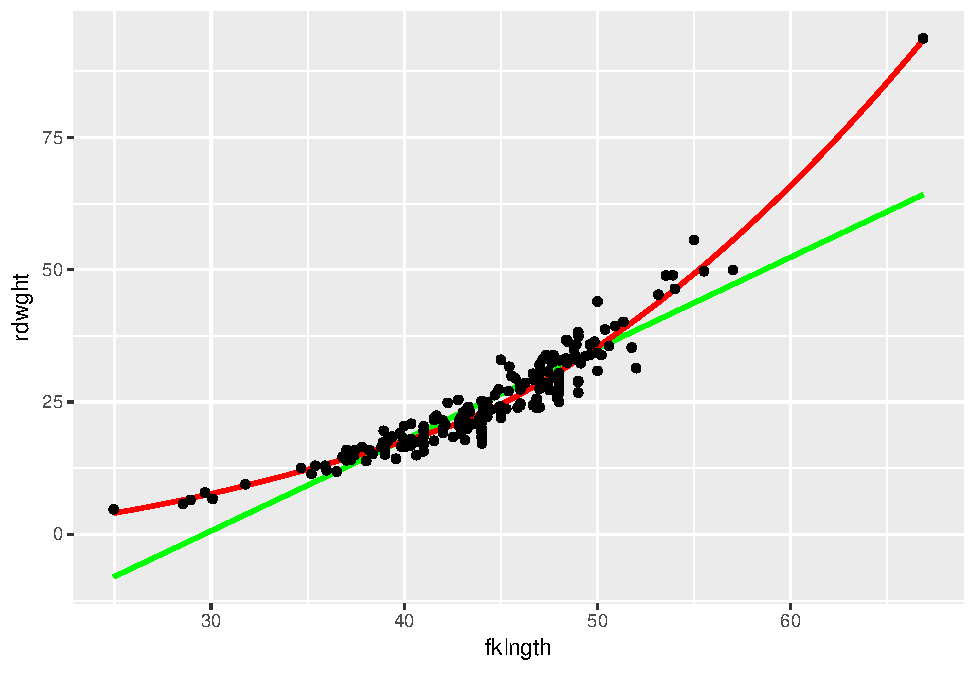
\includegraphics{Labs_BIO4158_files/figure-latex/stur-2-1.pdf}
\caption{\label{fig:stur-2}Scatter plot of Weight as a function of length in sturgeons}
\end{figure}

\begin{itemize}
\tightlist
\item
  Does this curve suggest a good correlation between the two? Based on visual inspection, does the relationship between these two variables appear linear?
\end{itemize}

There is some evidence of nonlinearity, as the curve appears to have a positive second derivative (concave up). This notwithstanding, it does appear the two variables are highly correlated.

\begin{itemize}
\tightlist
\item
  Redo the scatterplot, but after logtransformation of both axes.
\end{itemize}

\begin{Shaded}
\begin{Highlighting}[]
\CommentTok{\# apply log transformation on defined graph}
\NormalTok{mygraph }\OperatorTok{+}\StringTok{ }\KeywordTok{scale\_x\_log10}\NormalTok{() }\OperatorTok{+}\StringTok{ }\KeywordTok{scale\_y\_log10}\NormalTok{()}
\end{Highlighting}
\end{Shaded}

\begin{figure}
\centering
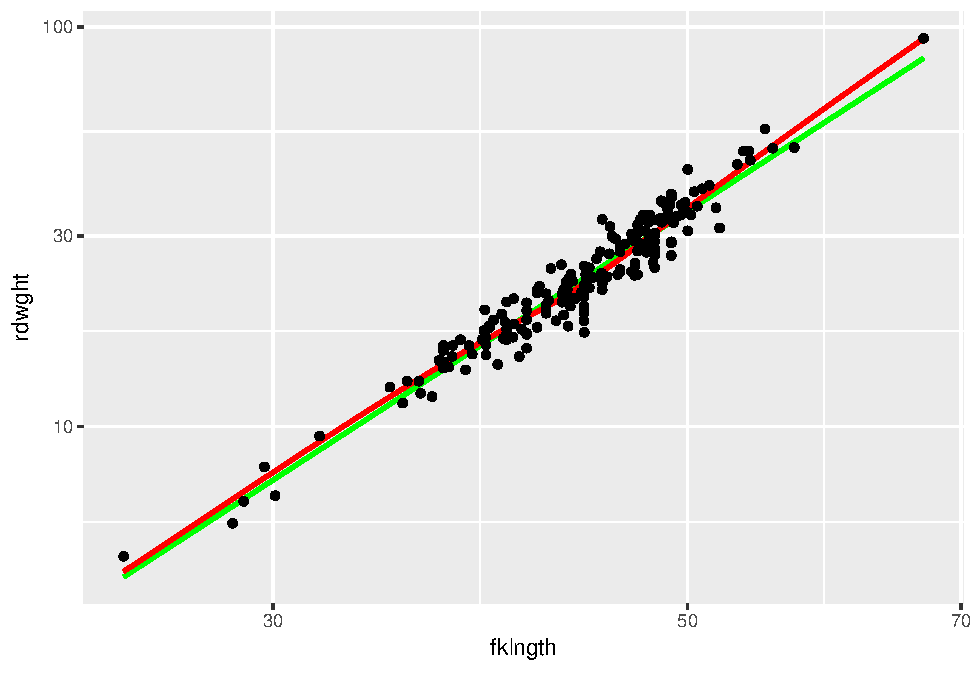
\includegraphics{Labs_BIO4158_files/figure-latex/stur-log-1.pdf}
\caption{\label{fig:stur-log}Plot weight-length in sturgeon using a log scale}
\end{figure}

Compare the diagrams before and after the transformation (Figs \ref{fig:stur-2} and \ref{fig:stur-log}). Since the relationship is more linear after transformation, correlation analysis should be done on the transformed data

\hypertarget{data-transformations-and-the-product-moment-correlation}{%
\section{Data transformations and the product-moment correlation}\label{data-transformations-and-the-product-moment-correlation}}

Recall that another assumption underlying significance testing of the product-moment correlation is that the distribution of the two variables in question is bivariate normal. We can test to see whether each of the two variables are normally distributed using the same procedures outlined in the exercise on two-sample comparisons. If the two variables are each normally distributed, then one is usually (relatively) safe in assuming the joint distribution is normal, although this needn't necessarily be true.

\begin{itemize}
\tightlist
\item
  Examine the distribution of the 4 variables (the two original variables and the log-transformed variables). What do you conclude from visual inspection of these plots?
\end{itemize}

The following graph contains the 4 QQ plots (\texttt{qqplot()}). It was produced by the code below that starts with the \texttt{par()} command to ensure that all 4 plots would appear together on the same page in 2 rows and 2 columns:

\begin{Shaded}
\begin{Highlighting}[]
\KeywordTok{par}\NormalTok{(}\DataTypeTok{mfrow =} \KeywordTok{c}\NormalTok{(}\DecValTok{2}\NormalTok{, }\DecValTok{2}\NormalTok{)) }\CommentTok{\# split graph in 4 (2 rows, 2 cols) filling by rows}
\KeywordTok{qqnorm}\NormalTok{(sturgeon}\OperatorTok{$}\NormalTok{fklngth, }\DataTypeTok{ylab =} \StringTok{"fklngth"}\NormalTok{)}
\KeywordTok{qqline}\NormalTok{(sturgeon}\OperatorTok{$}\NormalTok{fklngth)}
\KeywordTok{qqnorm}\NormalTok{(}\KeywordTok{log10}\NormalTok{(sturgeon}\OperatorTok{$}\NormalTok{fklngth), }\DataTypeTok{ylab =} \StringTok{"log10(fklngth)"}\NormalTok{)}
\KeywordTok{qqline}\NormalTok{(}\KeywordTok{log10}\NormalTok{(sturgeon}\OperatorTok{$}\NormalTok{fklngth))}
\KeywordTok{qqnorm}\NormalTok{(sturgeon}\OperatorTok{$}\NormalTok{rdwght, }\DataTypeTok{ylab =} \StringTok{"rdwght"}\NormalTok{)}
\KeywordTok{qqline}\NormalTok{(sturgeon}\OperatorTok{$}\NormalTok{rdwght)}
\KeywordTok{qqnorm}\NormalTok{(}\KeywordTok{log10}\NormalTok{(sturgeon}\OperatorTok{$}\NormalTok{rdwght), }\DataTypeTok{ylab =} \StringTok{"log10(rdwgth)"}\NormalTok{)}
\KeywordTok{qqline}\NormalTok{(}\KeywordTok{log10}\NormalTok{(sturgeon}\OperatorTok{$}\NormalTok{rdwght))}
\end{Highlighting}
\end{Shaded}

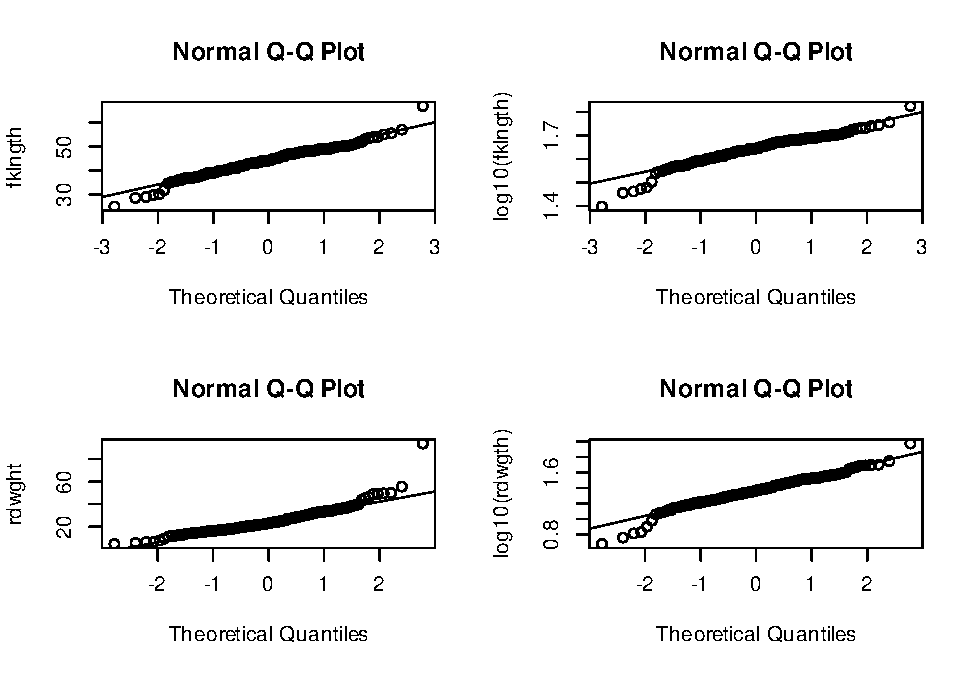
\includegraphics{Labs_BIO4158_files/figure-latex/stur-4hist-1.pdf}

\begin{Shaded}
\begin{Highlighting}[]
\KeywordTok{par}\NormalTok{(}\DataTypeTok{mfrow =} \KeywordTok{c}\NormalTok{(}\DecValTok{1}\NormalTok{, }\DecValTok{1}\NormalTok{)) }\CommentTok{\# redefine plotting area to 1 plot}
\end{Highlighting}
\end{Shaded}

None of these distributions are perfectly normal, but deviations are mostly minor.

\begin{itemize}
\tightlist
\item
  To generate a scatterplot matrix of all pairs of variables, with linear regression and lowess traces, you can use \texttt{scatterplotMatrix} from \texttt{car} `r emo::ji(``package'').
\end{itemize}

\begin{Shaded}
\begin{Highlighting}[]
\KeywordTok{scatterplotMatrix}\NormalTok{(}
  \OperatorTok{\textasciitilde{}}\StringTok{ }\NormalTok{fklngth }\OperatorTok{+}\StringTok{ }\KeywordTok{log10}\NormalTok{(fklngth) }\OperatorTok{+}\StringTok{ }\NormalTok{rdwght }\OperatorTok{+}\StringTok{ }\KeywordTok{log10}\NormalTok{(rdwght),}
  \DataTypeTok{data =}\NormalTok{ sturgeon,}
  \DataTypeTok{smooth =} \OtherTok{TRUE}\NormalTok{, }\DataTypeTok{diagonal =} \StringTok{"density"}
\NormalTok{)}
\end{Highlighting}
\end{Shaded}

\begin{verbatim}
## Warning in applyDefaults(diagonal, defaults = list(method =
## "adaptiveDensity"), : unnamed diag arguments, will be ignored
\end{verbatim}

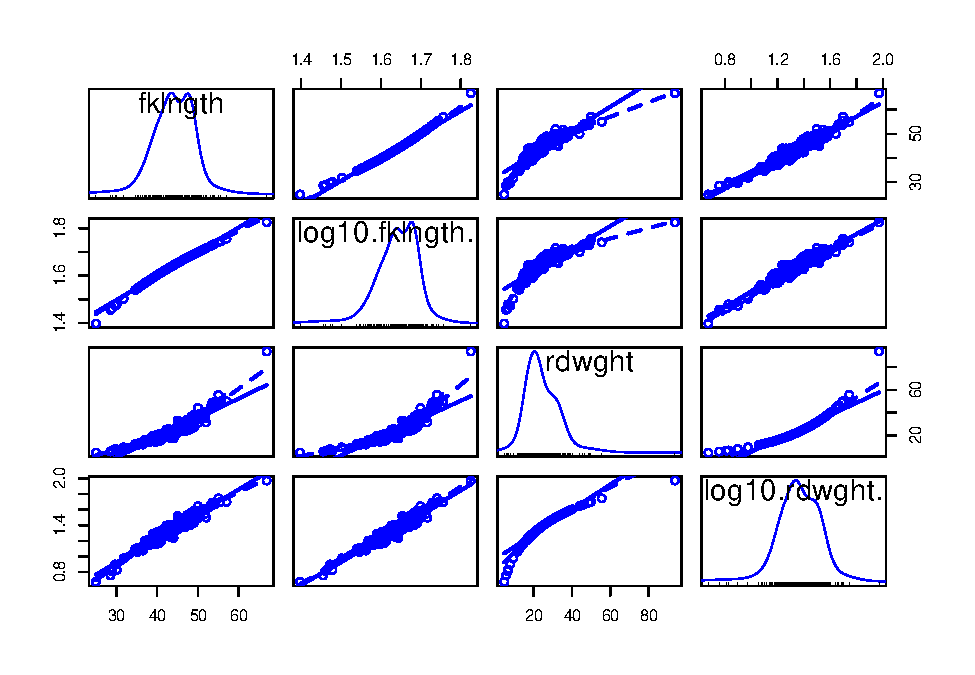
\includegraphics{Labs_BIO4158_files/figure-latex/stur-scatmat-1.pdf}

\begin{itemize}
\tightlist
\item
  Next, calculate the Pearson product-moment correlation between each pair (untransformed and log transformed) using the \texttt{cor()} command. However, to do this, it will be easier if you first add your transformed data as columns in the sturgeon data frame.
\end{itemize}

\begin{Shaded}
\begin{Highlighting}[]
\NormalTok{sturgeon}\OperatorTok{$}\NormalTok{lfklngth \textless{}{-}}\StringTok{ }\KeywordTok{with}\NormalTok{(sturgeon, }\KeywordTok{log10}\NormalTok{(fklngth))}
\NormalTok{sturgeon}\OperatorTok{$}\NormalTok{lrdwght \textless{}{-}}\StringTok{ }\KeywordTok{log10}\NormalTok{(sturgeon}\OperatorTok{$}\NormalTok{rdwght)}
\end{Highlighting}
\end{Shaded}

Then you can get the correlation matrix by:

\begin{Shaded}
\begin{Highlighting}[]
\KeywordTok{cor}\NormalTok{(sturgeon[, }\KeywordTok{c}\NormalTok{(}\StringTok{"fklngth"}\NormalTok{, }\StringTok{"lfklngth"}\NormalTok{, }\StringTok{"lrdwght"}\NormalTok{, }\StringTok{"rdwght"}\NormalTok{)], }\DataTypeTok{use =} \StringTok{"complete.obs"}\NormalTok{)}
\end{Highlighting}
\end{Shaded}

Note the \texttt{use="complete.obs"} parameter. It tells R to keep only lines of the data frame where all variables were measured. If there are missing data, some lines will be removed, but correlations will be calculated for the same subset of cases for all pairs of variables. One could use, instead, \texttt{use="pairwise.complete.obs"} , to tell R to only eliminate observations when values are missing for this particular pair of variables. In this situation, if there are missing values in the data frame, the sample size for pairwise correlations will vary. In general, I recommend you use the option \texttt{use="complete.obs"}, unless you have so many missing values that it eliminates the majority of your data.

\begin{itemize}
\tightlist
\item
  Why is the correlation between the untransformed variables smaller than between the transformed variables?
\end{itemize}

\begin{Shaded}
\begin{Highlighting}[]
\KeywordTok{cor}\NormalTok{(sturgeon[, }\KeywordTok{c}\NormalTok{(}\StringTok{"fklngth"}\NormalTok{, }\StringTok{"lfklngth"}\NormalTok{, }\StringTok{"lrdwght"}\NormalTok{, }\StringTok{"rdwght"}\NormalTok{)], }\DataTypeTok{use =} \StringTok{"complete.obs"}\NormalTok{)}
\end{Highlighting}
\end{Shaded}

\begin{verbatim}
##            fklngth  lfklngth   lrdwght    rdwght
## fklngth  1.0000000 0.9921435 0.9645108 0.9175435
## lfklngth 0.9921435 1.0000000 0.9670139 0.8756203
## lrdwght  0.9645108 0.9670139 1.0000000 0.9265513
## rdwght   0.9175435 0.8756203 0.9265513 1.0000000
\end{verbatim}

Several things should be noted here.

\begin{enumerate}
\def\labelenumi{\arabic{enumi}.}
\tightlist
\item
  the correlation between fork length and round weight is high, regardless of which variables are used: so as might be expected, heavier fish are also longer, and vice versa
\item
  the correlation is greater for the transformed variables than the untransformed variables.
\end{enumerate}

\textbf{Why?} Because the correlation coefficient is inversely proportional to the amount of scatter around a straight line. If the relationship is curvilinear (as it is for the untransformed data), the scatter around a straight line will be greater than if the relationship is linear.
Hence, the correlation coefficient will be smaller.

\hypertarget{testing-the-significance-of-correlations-and-bonferroni-probabilities}{%
\section{Testing the significance of correlations and Bonferroni probabilities}\label{testing-the-significance-of-correlations-and-bonferroni-probabilities}}

It's possible to test the significance of individual correlations using the commands window.
As an example, let's try testing the significance of the correlation between lfklngth and rdwght (the smallest correlation in the above table).

\begin{itemize}
\tightlist
\item
  In the R script window, enter the following to test the correlation
  between \texttt{lfkgnth} and \texttt{rdwght} :
\end{itemize}

\begin{Shaded}
\begin{Highlighting}[]
\KeywordTok{cor.test}\NormalTok{(}
\NormalTok{  sturgeon}\OperatorTok{$}\NormalTok{lfklngth, sturgeon}\OperatorTok{$}\NormalTok{rdwght,}
  \DataTypeTok{alternative =} \StringTok{"two.sided"}\NormalTok{,}
  \DataTypeTok{method =} \StringTok{"pearson"}
\NormalTok{)}
\end{Highlighting}
\end{Shaded}

\begin{verbatim}
## 
##  Pearson's product-moment correlation
## 
## data:  sturgeon$lfklngth and sturgeon$rdwght
## t = 24.322, df = 180, p-value < 2.2e-16
## alternative hypothesis: true correlation is not equal to 0
## 95 percent confidence interval:
##  0.8367345 0.9057199
## sample estimates:
##       cor 
## 0.8756203
\end{verbatim}

We see here that the correlation is highly significant (\(p< 2.2e-16\)),
which is no surprise given how high the correlation coefficient is (0.8756).

It's important to bear in mind that when you are estimating correlations, the probability of finding any one correlation that is \emph{``significant''} by pure chance increases with the number of pairwise correlations examined. Suppose, for example, that you have five variables; there are then a total of 10 possible pairwise correlations, and from this set, you would probably not be surprised to find at least one that is ``significant'' purely by chance. One way of avoiding the problem is to adjust individual \(\alpha\) levels for pairwise correlations by dividing by the number of comparisons, k, such that: \(\alpha' = \frac{\alpha}{k}\) (Bonferroni probabilities), i.e.~if initially, \(\alpha = 0.05\) and there are a total of 10 comparisons, then \(\alpha'= 0.005\).

In the above example where we examined correlations between
\texttt{fklngth} and \texttt{rdwght} and their \texttt{log}, it would be appropriate to adjust
the \(\alpha\) at which significance is tested by the total number of
correlations in the matrix (in this case, 6, so \(\alpha'=0.0083\)). Does your
decision about the significance of the correlation between \texttt{lfklngth} and
\texttt{rdwght} change?

\hypertarget{non-parametric-correlations-spearmans-rank-and-kendalls-tau}{%
\section{\texorpdfstring{Non-parametric correlations: Spearman's rank and Kendall's \(\tau\)}{Non-parametric correlations: Spearman's rank and Kendall's \textbackslash tau}}\label{non-parametric-correlations-spearmans-rank-and-kendalls-tau}}

The analysis done with the sturgeon data in the section above suggests that one of the assumptions of correlation, namely, bivariate normality, may not be valid for \texttt{fklngth} and \texttt{rdwght} nor for the log transforms of these variables. Finding an appropriate transformation is sometimes like looking for a needle in a haystack; indeed, it can be much worse simply because for some distributions, there is no transformation that will normalize the data. In such cases, the best option may be to go to a non-parametric analysis that does not assume bivariate normality or linearity. All such correlations are based on the ranks rather than the data themselves: two options available in
R are Spearman and Kendall's \(\tau\) (tau).

\begin{itemize}
\tightlist
\item
  Test the correlation between \texttt{fklngth} and \texttt{rdwght} using both the Spearman and Kendall's tau. The following commands will produce the correlations:
\end{itemize}

\begin{Shaded}
\begin{Highlighting}[]
\KeywordTok{cor.test}\NormalTok{(}
\NormalTok{  sturgeon}\OperatorTok{$}\NormalTok{lfklngth, sturgeon}\OperatorTok{$}\NormalTok{rdwght,}
  \DataTypeTok{alternative =} \StringTok{"two.sided"}\NormalTok{,}
  \DataTypeTok{method =} \StringTok{"spearman"}
\NormalTok{)}
\end{Highlighting}
\end{Shaded}

\begin{verbatim}
## Warning in cor.test.default(sturgeon$lfklngth, sturgeon$rdwght, alternative =
## "two.sided", : Cannot compute exact p-value with ties
\end{verbatim}

\begin{verbatim}
## 
##  Spearman's rank correlation rho
## 
## data:  sturgeon$lfklngth and sturgeon$rdwght
## S = 47971, p-value < 2.2e-16
## alternative hypothesis: true rho is not equal to 0
## sample estimates:
##       rho 
## 0.9522546
\end{verbatim}

\begin{Shaded}
\begin{Highlighting}[]
\KeywordTok{cor.test}\NormalTok{(}
\NormalTok{  sturgeon}\OperatorTok{$}\NormalTok{lfklngth, sturgeon}\OperatorTok{$}\NormalTok{rdwght,}
  \DataTypeTok{alternative =} \StringTok{"two.sided"}\NormalTok{,}
  \DataTypeTok{method =} \StringTok{"kendall"}
\NormalTok{)}
\end{Highlighting}
\end{Shaded}

\begin{verbatim}
## 
##  Kendall's rank correlation tau
## 
## data:  sturgeon$lfklngth and sturgeon$rdwght
## z = 16.358, p-value < 2.2e-16
## alternative hypothesis: true tau is not equal to 0
## sample estimates:
##       tau 
## 0.8208065
\end{verbatim}

Contrast these results with those obtained using the Pearson product-moment correlation. Why the difference?

Test the non-parametric correlations on pairs of the transformed variables. You should immediately note that the non-parametric correlations are identical for untransformed and transformed variables. This is because we are using the ranks, rather than the raw data, and the rank ordering of the data does not change when a transformation is applied to the raw values.

Note that the correlations for Kendall's tau (0.820) are lower than for the Spearman rank (0.952) correlation. This is because Kendall's gives more weight to ranks that are far apart, whereas Spearman's weights each rank equally. Generally, Kendalls's is more appropriate when there is more uncertainty about the reliability of close ranks.

The sturgeons in this sample were collected using nets and baited hooks of a certain size. What impact do you think this method of collection had on the shapes of the distributions of \texttt{fklngth} and \texttt{rdwght} ? Under these circumstances, do you think correlation analysis is appropriate at all?

Note that correlation analysis assumes that each variable is \emph{randomly sampled}. In the case of sturgeon, this is not the case: baited hooks and nets will only catch sturgeon above a certain minimum size. Note that in the sample, there are no small sturgeons, since the fishing gear targets only larger fish. Thus, we should be very wary of the correlation coefficients associated with our analysis, as the inclusion of smaller fish may well change our estimate of these correlations.

\hypertarget{simple-linear-regression}{%
\section{Simple linear regression}\label{simple-linear-regression}}

In correlation analysis we are interested in how pairs of variables covary: However, in regression analysis, we are attempting to estimate a model that predicts a variable (the dependent variable) from another variable (the independent variable).

As with any statistical analysis, the best way to begin is by looking at your data.
If you are interested in the relationship between two variables, say, Y and X, produce a plot of Y versus X just to get a ``feel'' for the relationship.

\begin{itemize}
\tightlist
\item
  The data file \texttt{sturgeon.csv} contains data for sturgeons collected from 1978-1980 at Cumberland House, Saskatchewan and The Pas, Manitoba. Make a scatterplot of \texttt{fklngth} (the dependent variable) versus \texttt{age} (the independent variable) for males and add a linear regression and a loess smoother. What do you conclude from this plot?
\end{itemize}

\begin{Shaded}
\begin{Highlighting}[]
\NormalTok{sturgeon.male \textless{}{-}}\StringTok{ }\KeywordTok{subset}\NormalTok{(sturgeon, }\DataTypeTok{subset =}\NormalTok{ sex }\OperatorTok{==}\StringTok{ "MALE"}\NormalTok{)}
\NormalTok{mygraph \textless{}{-}}\StringTok{ }\KeywordTok{ggplot}\NormalTok{(}
  \DataTypeTok{data =}\NormalTok{ sturgeon.male, }\CommentTok{\# source of data}
  \KeywordTok{aes}\NormalTok{(}\DataTypeTok{x =}\NormalTok{ age, }\DataTypeTok{y =}\NormalTok{ fklngth)}
\NormalTok{) }\CommentTok{\# aesthetics: y=fklngth, x=rdwght}
\CommentTok{\# plot data points, regression, loess trace}
\NormalTok{mygraph \textless{}{-}}\StringTok{ }\NormalTok{mygraph }\OperatorTok{+}
\StringTok{  }\KeywordTok{stat\_smooth}\NormalTok{(}\DataTypeTok{method =}\NormalTok{ lm, }\DataTypeTok{se =} \OtherTok{FALSE}\NormalTok{, }\DataTypeTok{color =} \StringTok{"green"}\NormalTok{) }\OperatorTok{+}\StringTok{ }\CommentTok{\# add linear regression, but no SE shading}
\StringTok{  }\KeywordTok{stat\_smooth}\NormalTok{(}\DataTypeTok{color =} \StringTok{"red"}\NormalTok{) }\OperatorTok{+}\StringTok{ }\CommentTok{\# add loess}
\StringTok{  }\KeywordTok{geom\_point}\NormalTok{() }\CommentTok{\# add data points}
\NormalTok{mygraph }\CommentTok{\# display graph}
\end{Highlighting}
\end{Shaded}

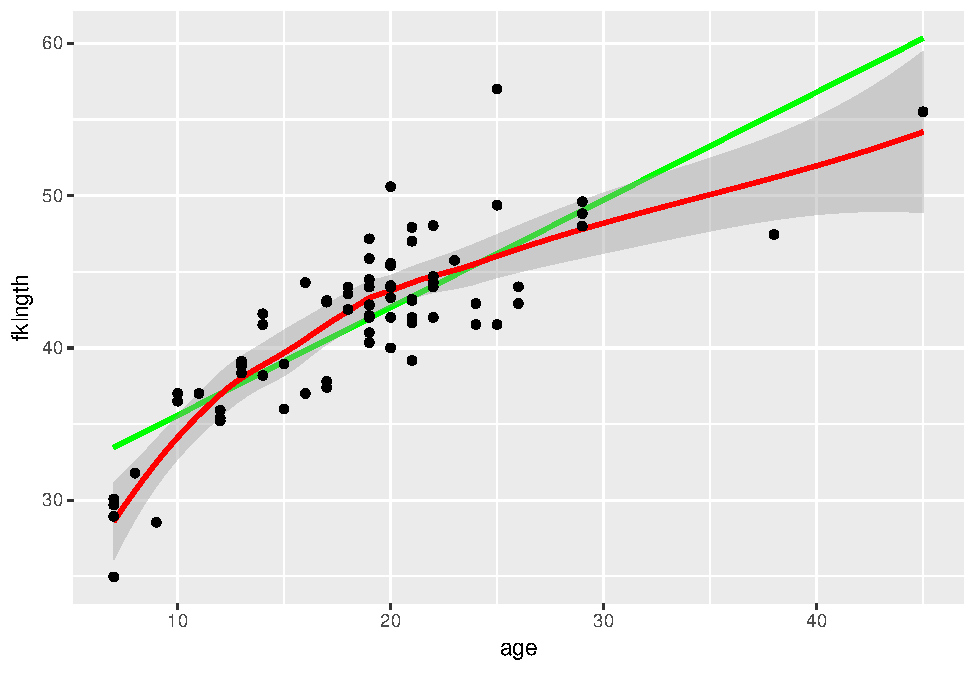
\includegraphics{Labs_BIO4158_files/figure-latex/sturlm-1-1.pdf}

This suggests that the relationship between age and fork length is not linear.

Suppose that we want to know the growth rate of male sturgeon. One estimate (perhaps not a very good one) of the growth rate is given by the slope of the fork length - age regression.

First, let's run the regression with the lm() command, and save its
results in an object called \texttt{RegModel.1}.

\begin{Shaded}
\begin{Highlighting}[]
\NormalTok{RegModel}\FloatTok{.1}\NormalTok{ \textless{}{-}}\StringTok{ }\KeywordTok{lm}\NormalTok{(fklngth }\OperatorTok{\textasciitilde{}}\StringTok{ }\NormalTok{age, }\DataTypeTok{data =}\NormalTok{ sturgeon.male)}
\end{Highlighting}
\end{Shaded}

Nothing appears on the screen, but don't worry, it all got saved in memory.
To see the statistical results, type:

\begin{Shaded}
\begin{Highlighting}[]
\KeywordTok{summary}\NormalTok{(RegModel}\FloatTok{.1}\NormalTok{)}
\end{Highlighting}
\end{Shaded}

\begin{verbatim}
## 
## Call:
## lm(formula = fklngth ~ age, data = sturgeon.male)
## 
## Residuals:
##     Min      1Q  Median      3Q     Max 
## -8.4936 -2.2263  0.1849  1.7526 10.8234 
## 
## Coefficients:
##             Estimate Std. Error t value Pr(>|t|)    
## (Intercept) 28.50359    1.16873   24.39   <2e-16 ***
## age          0.70724    0.05888   12.01   <2e-16 ***
## ---
## Signif. codes:  0 '***' 0.001 '**' 0.01 '*' 0.05 '.' 0.1 ' ' 1
## 
## Residual standard error: 3.307 on 73 degrees of freedom
##   (5 observations deleted due to missingness)
## Multiple R-squared:  0.664,  Adjusted R-squared:  0.6594 
## F-statistic: 144.3 on 1 and 73 DF,  p-value: < 2.2e-16
\end{verbatim}

R output gives you:

\begin{enumerate}
\def\labelenumi{\arabic{enumi}.}
\tightlist
\item
  \texttt{Call:} A friendly reminder of the model fitted and the data used.
\item
  \texttt{Residuals:} General statistics about the residuals around the fitted model.
\item
  \texttt{Coefficients:} Fitted model parameter estimates, standard errors, t values and associated probabilities.
\item
  \texttt{Residual\ standard\ error:} Square root of the residual variance.
\item
  \texttt{Multiple\ R-squared:} Coefficient of determination. It corresponds to the proportion of the total variance of the dependent variable that is accounted for by the regression (i.e.~by the independent variable)
\item
  \texttt{Adjusted\ R-squared:} The adjusted R-squared accounts for the number of parameters in the model. If you want to compare the performance of several models with different numbers of parameters, this is the one to use
\item
  \texttt{F-statistic:} This is the test of the overall significance of the model. In the simple regression case, this is the same as the test of the slope of the
  regression.
\end{enumerate}

The estimated regression equation is therefore:

\[ Fklngth = 28.50359 + 0.70724 * age\]

Given the highly significant F-value of the model (or equivalently the highly significant t-value for the slope of the line), we reject the null hypothesis that there is no relationship between fork length and age.

\hypertarget{testing-regression-assumptions}{%
\subsection{Testing regression assumptions}\label{testing-regression-assumptions}}

Simple model I regression makes four assumptions:

\begin{enumerate}
\def\labelenumi{\arabic{enumi}.}
\tightlist
\item
  the X variable is measured without error;
\item
  the relationship between Y and X is linear;
\item
  that for any value of X, the Y's are independently and normally distributed;
\item
  the variance of Y for fixed X is independent of X.
\end{enumerate}

Having done the regression, we can now test the assumptions.
For most biological data, the first assumption is almost never valid; usually there is error in both Y and X. This means that in general, slope estimates are biased, but predicted values are unbiased. However, so long as the error in X is small relative to the range of X in your data, the fact that X has an associated error is not likely to influence the outcome dramatically. On the other hand, if there is substantial error in X, regression results based on a model I regression may give poor estimates of the functional relationship between Y and X. In this case, more sophisticated regression procedures must be employed which are, unfortunately, beyond the scope of this course.

The other assumptions of a model I regression can, however, be tested, or at least evaluated visually. The \texttt{plot()} command can display diagnostics for linear models.

\begin{Shaded}
\begin{Highlighting}[]
\KeywordTok{par}\NormalTok{(}\DataTypeTok{mfrow =} \KeywordTok{c}\NormalTok{(}\DecValTok{2}\NormalTok{, }\DecValTok{2}\NormalTok{), }\DataTypeTok{las =} \DecValTok{1}\NormalTok{)}
\KeywordTok{plot}\NormalTok{(RegModel}\FloatTok{.1}\NormalTok{)}
\end{Highlighting}
\end{Shaded}

The \texttt{par()} command is used here to tell R to display 2 rows and 2 columns of graphs per page (there are 4 diagnostic graphs for linear models generated automatically), and the last statement is to tell R to rotate the labels of the Y axis so that they are perpendicular to the Y axis. (Yes, I know, this is not at all obvious.)

You will get:
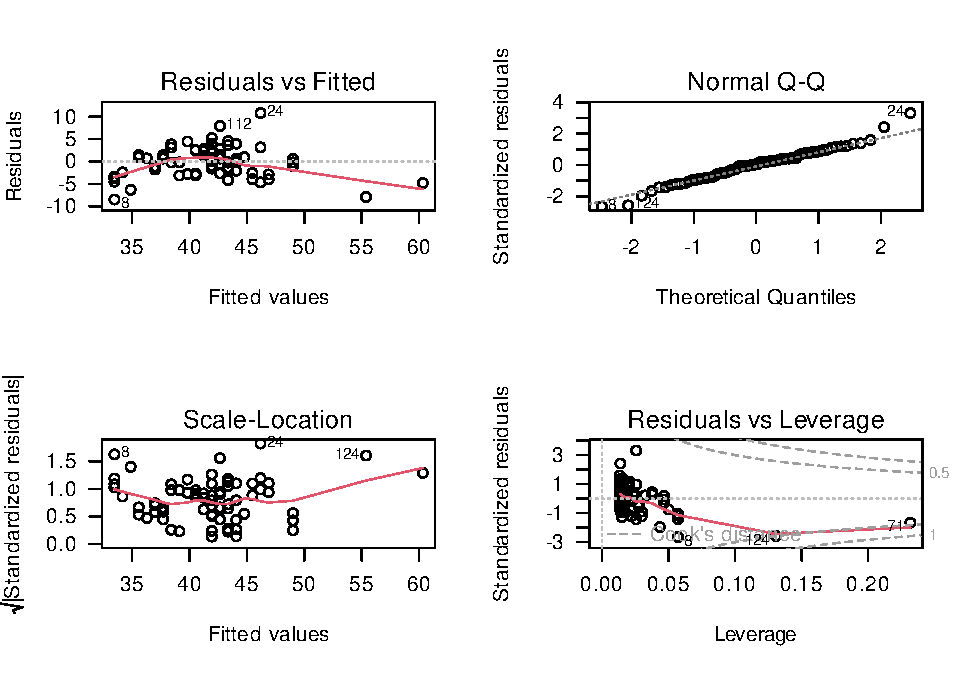
\includegraphics{Labs_BIO4158_files/figure-latex/sturlmv-1eval-1.pdf}

\begin{enumerate}
\def\labelenumi{\arabic{enumi}.}
\tightlist
\item
  \textbf{Upper left} tell you about linearity, normality, and homoscedasticity of the residuals. It shows the deviations around the regression vs the predicted values. Remember that the scatterplot ( fklngth vs age ) suggested that the relationship between fork length and age is not linear. Very young and very old sturgeons tended to fall under the line, and fish of average age tended to be a bit above the line. This is exactly what the residual vs fitted plot shows. The red line is a lowess trace through these data. If the relationship was linear, it would be approximately flat and close to 0. The scatter of residuals tells you a bit about their normality and homoscedasticity, although this graph is not the best way to look at these properties. The next two are better.
\item
  \textbf{Upper right} is to assess the normality of the residuals. It is a QQ plot of the residuals . If the residuals were normally distributed, they would fall very close to the diagonal line. Here, we see it is mostly the case, except in the tails
\item
  \textbf{Bottom left} titled Scale-Location, helps with assessing homoscedasticity. It plots the square root of the absolute value of the standardized residual (residual divided by the standard error of the residuals, this scales the residuals so that their variance is 1 ) as a function of the fitted value. This graph can help you visualize whether the spread of the residuals is constant or not. If residuals are homoscedastic, then the average will not change with increasing fitted values. Here, there is slight variability, but it is not monotonous (i.e.~it does not increase or decrease systematically) and there is no strong evidence against the assumption of homoscedasticity.
\item
  \textbf{Bottom right} plots the residuals as a function of leverage and can help detecting the presence of outliers or points that have a very strong influence on the regression results. The leverage of a point measures how far it is from the other points, but only with respect to the independent variable. In the case of simple linear regression, it is a function of the difference between the observation and the mean of the independent variable. You should look more closely at any observation with a leverage value that is greater than: \(2(k+1)/n\), where \$\(k\) is the number of independent variables (here 1), and \(n\) is the number of observations. In this case there is 1 independent variable, 75 observations, and points with a leverage higher than 0.053 may warrant particular scrutiny. The plot also gives you information about how the removal of a point from the data set would change the predictions. This is measured by the Cook's distance, illustrated by the red lines on the plot. A data point with a Cook distance larger than 1 has a large influence.
\end{enumerate}

\begin{rmdwarning}
Note that R automatically labels the most extreme cases on each of these 4 plots. It does not mean that these cases are outliers, or that you necessarily need be concerned with them. In any data set, there will always be a minimum and a maximum residual.
\end{rmdwarning}

The R package \texttt{performance} offers a new and updated version of those graphs with colours and more plots to help visually assess the assumptions with the function \texttt{model\_check()}

\begin{Shaded}
\begin{Highlighting}[]
\KeywordTok{check\_model}\NormalTok{(RegModel}\FloatTok{.1}\NormalTok{)}
\end{Highlighting}
\end{Shaded}

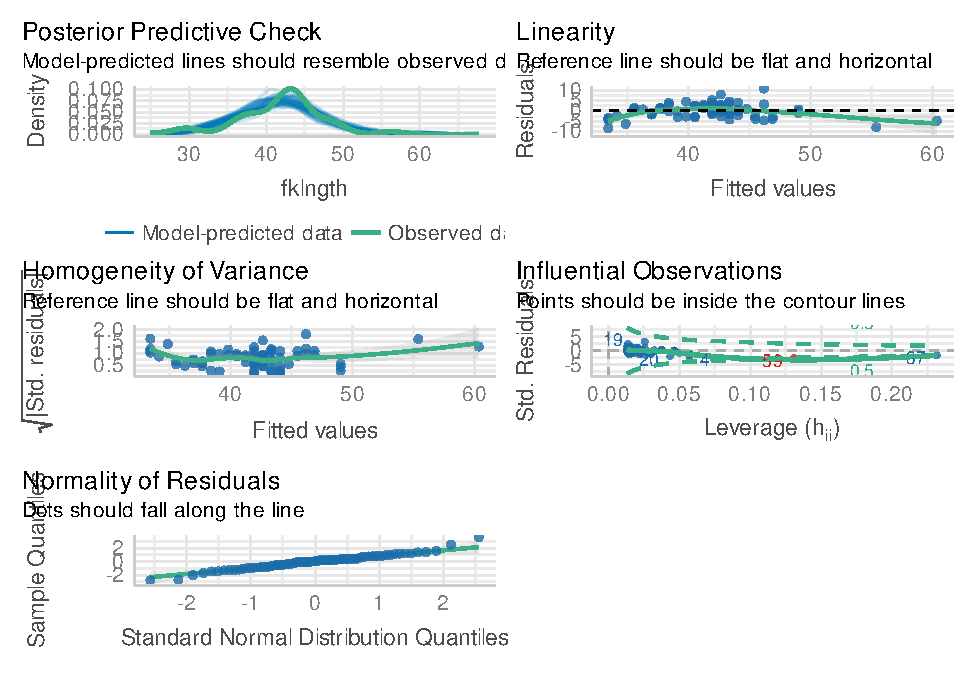
\includegraphics{Labs_BIO4158_files/figure-latex/unnamed-chunk-29-1.pdf}

So, what is the verdict about the linear regression between \texttt{fklngth} and \texttt{age} ? It fails the linearity, possibly fails the normality, passes homoscedasticity, and this does not seem to be too strongly affected by some bizarre points.

\hypertarget{formal-tests-of-regression-assumptions}{%
\subsection{Formal tests of regression assumptions}\label{formal-tests-of-regression-assumptions}}

In my practice, I seldom use formal tests of regression assumptions and mostly rely on graphs of the residuals to guide my decisions. To my knowledge, this is what most biologists and data analysts do. However, in my early analyst life I was not always confident that I was interpreting these graphs correctly and wished that I had a formal test or a statistic quantifying the degree of deviation from the regression assumptions.

The \texttt{lmtest} R package, not part of the base R installation, but available from CRAN, contains a number of tests for linearity and homoscedasticity. And one can test for normality using the Shapiro-Wilk test seen previously.

First, you need to load (and maybe install) the \texttt{lmtest} package.

\begin{Shaded}
\begin{Highlighting}[]
\KeywordTok{library}\NormalTok{(lmtest)}
\end{Highlighting}
\end{Shaded}

\begin{rmdcode}
Run the following commands
\end{rmdcode}

\begin{Shaded}
\begin{Highlighting}[]
\KeywordTok{bptest}\NormalTok{(RegModel}\FloatTok{.1}\NormalTok{)}
\end{Highlighting}
\end{Shaded}

\begin{verbatim}
## 
##  studentized Breusch-Pagan test
## 
## data:  RegModel.1
## BP = 1.1765, df = 1, p-value = 0.2781
\end{verbatim}

The Breusch-Pagan test examines whether the variability of the residuals is constant with respect to increasing fitted values. A low p value is indicative of heteroscedasticity. Here, the p value is high, and supports my visual assessment that the homoscedasticity assumption is met by these data.

\begin{Shaded}
\begin{Highlighting}[]
\KeywordTok{dwtest}\NormalTok{(RegModel}\FloatTok{.1}\NormalTok{)}
\end{Highlighting}
\end{Shaded}

\begin{verbatim}
## 
##  Durbin-Watson test
## 
## data:  RegModel.1
## DW = 2.242, p-value = 0.8489
## alternative hypothesis: true autocorrelation is greater than 0
\end{verbatim}

The Durbin-Watson test can detect serial autocorrelation in the residuals. Under the assumption of no autocorrelation, the D statistic is 2. This test can detect violation of independence of observations (residuals), although it is not foolproof. Here there is no problem identified.

\begin{Shaded}
\begin{Highlighting}[]
\KeywordTok{resettest}\NormalTok{(RegModel}\FloatTok{.1}\NormalTok{)}
\end{Highlighting}
\end{Shaded}

\begin{verbatim}
## 
##  RESET test
## 
## data:  RegModel.1
## RESET = 14.544, df1 = 2, df2 = 71, p-value = 5.082e-06
\end{verbatim}

The RESET test is a test of the assumption of linearity. If the linearity assumption is met, the RESET statistic will be close to 1. Here, the statistic is much larger (14.54), and very highly significant. This confirms our visual assessment that the relationship is not linear.

\begin{Shaded}
\begin{Highlighting}[]
\KeywordTok{shapiro.test}\NormalTok{(}\KeywordTok{residuals}\NormalTok{(RegModel}\FloatTok{.1}\NormalTok{))}
\end{Highlighting}
\end{Shaded}

\begin{verbatim}
## 
##  Shapiro-Wilk normality test
## 
## data:  residuals(RegModel.1)
## W = 0.98037, p-value = 0.2961
\end{verbatim}

The Shapiro-Wilk normality test on the residual confirms that
the deviation from normality of the residuals is not large.

\hypertarget{data-transformations-in-regression}{%
\section{Data transformations in regression}\label{data-transformations-in-regression}}

The analysis above revealed that the linearity assumption underlying regression analysis is not met by the \texttt{fklngth} - \texttt{age} data. If we want to use regression analysis, data transformations are required:

Let's plot the log-transformed data

\begin{Shaded}
\begin{Highlighting}[]
\KeywordTok{par}\NormalTok{(}\DataTypeTok{mfrow =} \KeywordTok{c}\NormalTok{(}\DecValTok{1}\NormalTok{, }\DecValTok{1}\NormalTok{), }\DataTypeTok{las =} \DecValTok{1}\NormalTok{)}
\KeywordTok{ggplot}\NormalTok{(}
  \DataTypeTok{data =}\NormalTok{ sturgeon.male,}
  \KeywordTok{aes}\NormalTok{(}\DataTypeTok{x =} \KeywordTok{log10}\NormalTok{(age), }\DataTypeTok{y =} \KeywordTok{log10}\NormalTok{(fklngth))}
\NormalTok{) }\OperatorTok{+}
\StringTok{  }\KeywordTok{geom\_smooth}\NormalTok{(}\DataTypeTok{color =} \StringTok{"red"}\NormalTok{) }\OperatorTok{+}
\StringTok{  }\KeywordTok{geom\_smooth}\NormalTok{(}\DataTypeTok{method =} \StringTok{"lm"}\NormalTok{, }\DataTypeTok{se =} \OtherTok{FALSE}\NormalTok{, }\DataTypeTok{color =} \StringTok{"green"}\NormalTok{) }\OperatorTok{+}
\StringTok{  }\KeywordTok{geom\_point}\NormalTok{()}
\end{Highlighting}
\end{Shaded}

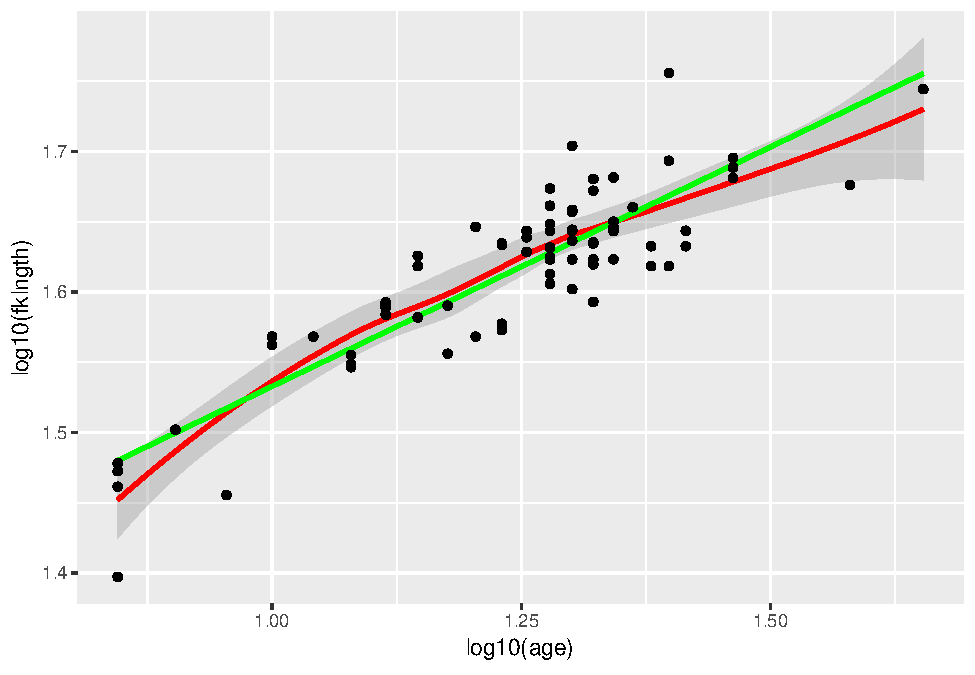
\includegraphics{Labs_BIO4158_files/figure-latex/sturtr-1-1.pdf}

We can fit the linear regression model on the log-transformed variables.

\begin{Shaded}
\begin{Highlighting}[]
\NormalTok{RegModel}\FloatTok{.2}\NormalTok{ \textless{}{-}}\StringTok{ }\KeywordTok{lm}\NormalTok{(}\KeywordTok{log10}\NormalTok{(fklngth) }\OperatorTok{\textasciitilde{}}\StringTok{ }\KeywordTok{log10}\NormalTok{(age), }\DataTypeTok{data =}\NormalTok{ sturgeon.male)}
\KeywordTok{summary}\NormalTok{(RegModel}\FloatTok{.2}\NormalTok{)}
\end{Highlighting}
\end{Shaded}

\begin{verbatim}
## 
## Call:
## lm(formula = log10(fklngth) ~ log10(age), data = sturgeon.male)
## 
## Residuals:
##       Min        1Q    Median        3Q       Max 
## -0.082794 -0.016837 -0.000719  0.021102  0.087446 
## 
## Coefficients:
##             Estimate Std. Error t value Pr(>|t|)    
## (Intercept)  1.19199    0.02723   43.77   <2e-16 ***
## log10(age)   0.34086    0.02168   15.72   <2e-16 ***
## ---
## Signif. codes:  0 '***' 0.001 '**' 0.01 '*' 0.05 '.' 0.1 ' ' 1
## 
## Residual standard error: 0.03015 on 73 degrees of freedom
##   (5 observations deleted due to missingness)
## Multiple R-squared:  0.772,  Adjusted R-squared:  0.7688 
## F-statistic: 247.1 on 1 and 73 DF,  p-value: < 2.2e-16
\end{verbatim}

Note that by using the log transformed data, the proportion of variation explained by the regression has increased by 10\% (from 0.664 to 0.772), a substantial increase. So the relationship has become more linear. Good. Let's look at the residual diagnostic plots:

\begin{Shaded}
\begin{Highlighting}[]
\KeywordTok{par}\NormalTok{(}\DataTypeTok{mfrow =} \KeywordTok{c}\NormalTok{(}\DecValTok{2}\NormalTok{, }\DecValTok{2}\NormalTok{), }\DataTypeTok{las =} \DecValTok{1}\NormalTok{)}
\KeywordTok{plot}\NormalTok{(RegModel}\FloatTok{.2}\NormalTok{)}
\end{Highlighting}
\end{Shaded}

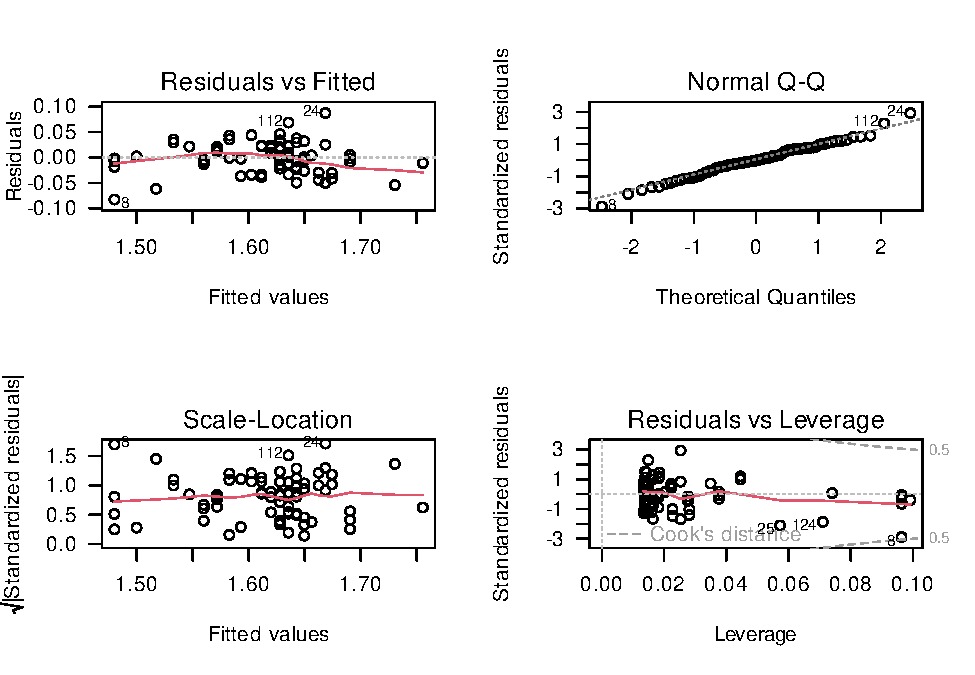
\includegraphics{Labs_BIO4158_files/figure-latex/sturtr-3-1.pdf}

\begin{Shaded}
\begin{Highlighting}[]
\KeywordTok{check\_model}\NormalTok{(RegModel}\FloatTok{.2}\NormalTok{)}
\end{Highlighting}
\end{Shaded}

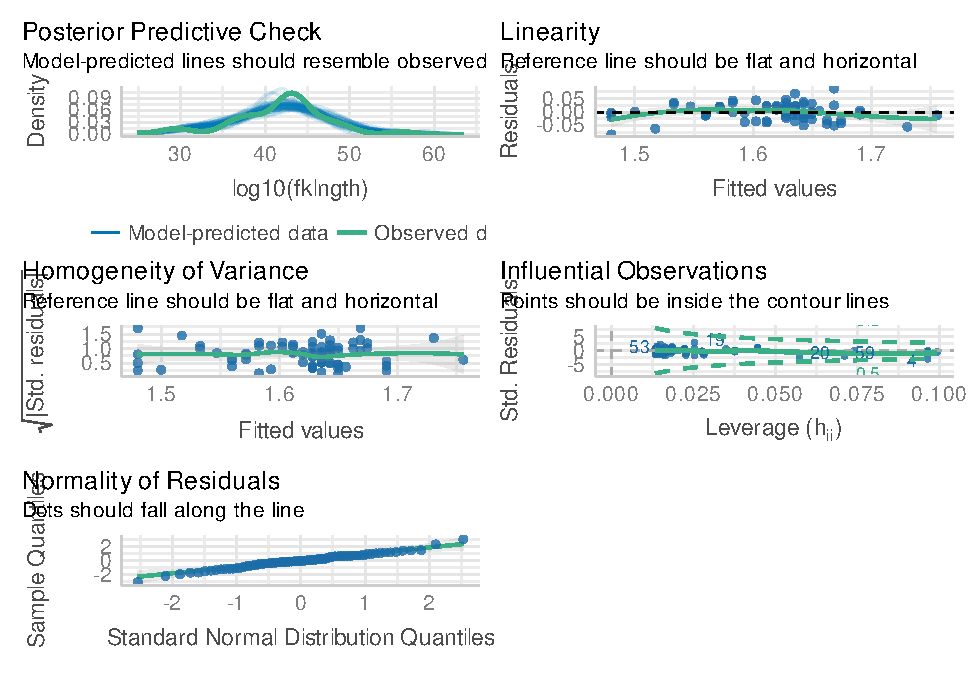
\includegraphics{Labs_BIO4158_files/figure-latex/sturtr-3-2.pdf}

So things appear a little better than before, although still not ideal. For example, the Residual vs fitted plot still suggests a potential nonlinearity. The QQ plot is nicer than before, indicating that residuals are more normally distributed after the log-log transformation. There is no indication of heteroscedasticity. And, although there are still a few points with somewhat high leverage, none have a Cook's distance above 0.5. It thus seems that transforming data improved things: more linear, more normal, less dependence on extreme data. Do the formal tests support this visual assessment?

\begin{Shaded}
\begin{Highlighting}[]
\KeywordTok{bptest}\NormalTok{(RegModel}\FloatTok{.2}\NormalTok{)}
\end{Highlighting}
\end{Shaded}

\begin{verbatim}
## 
##  studentized Breusch-Pagan test
## 
## data:  RegModel.2
## BP = 0.14282, df = 1, p-value = 0.7055
\end{verbatim}

\begin{Shaded}
\begin{Highlighting}[]
\KeywordTok{dwtest}\NormalTok{(RegModel}\FloatTok{.2}\NormalTok{)}
\end{Highlighting}
\end{Shaded}

\begin{verbatim}
## 
##  Durbin-Watson test
## 
## data:  RegModel.2
## DW = 2.1777, p-value = 0.6134
## alternative hypothesis: true autocorrelation is greater than 0
\end{verbatim}

\begin{Shaded}
\begin{Highlighting}[]
\KeywordTok{resettest}\NormalTok{(RegModel}\FloatTok{.2}\NormalTok{)}
\end{Highlighting}
\end{Shaded}

\begin{verbatim}
## 
##  RESET test
## 
## data:  RegModel.2
## RESET = 4.4413, df1 = 2, df2 = 71, p-value = 0.01523
\end{verbatim}

\begin{Shaded}
\begin{Highlighting}[]
\KeywordTok{shapiro.test}\NormalTok{(}\KeywordTok{residuals}\NormalTok{(RegModel}\FloatTok{.2}\NormalTok{))}
\end{Highlighting}
\end{Shaded}

\begin{verbatim}
## 
##  Shapiro-Wilk normality test
## 
## data:  residuals(RegModel.2)
## W = 0.98998, p-value = 0.8246
\end{verbatim}

Indeed, they do: residuals are still homoscedastic (Breusch-Pagan test), show no autocorrelation (Durbin-Watson test), are normal (Shapiro-Wilk test), and they are more linear (p value of the RESET test is now 0.015, instead of 0.000005). Linearity has improved, but is still violated somewhat.

\hypertarget{dealing-with-outliers}{%
\section{Dealing with outliers}\label{dealing-with-outliers}}

In this case, there are no real clear outliers. Yes, observations 8, 24, and 112 are labeled as the most extreme in the last set of residual diagnostic plots. But they are still within what I consider the ``reasonable'' range. But how does one define a limit to the reasonable? When is an extreme value a real outlier we have to deal with? Opinions vary about the issue, but I favor conservatism.

My rule is that, unless the value is clearly impossible or an error in data entry, I do not delete ``outliers''; rather, I analyze all my data. Why? Because, I want my data to reflect natural or real variability. Indeed, variability is often what interests biologists the most.

Keeping extreme values is the fairest way to proceed, but it often creates other issues. These values will often be the main reason why the data fail to meet the assumptions of the statistical analysis. One solution is to run the analysis with and without the outliers, and compare the results. In many cases, the two analyses will be qualitatively similar: the same conclusions will be reached, and the effect size will not be very different. Sometimes, however, this comparison will reveal that the presence of the outliers changes the story. The logical conclusion then is that the results depend on the outliers and that the data at hand are not very conclusive. As an example, let's rerun the analysis after eliminating observations labeled 8, 24, and 112.

\begin{Shaded}
\begin{Highlighting}[]
\NormalTok{RegModel}\FloatTok{.3}\NormalTok{ \textless{}{-}}\StringTok{ }\KeywordTok{lm}\NormalTok{(}\KeywordTok{log10}\NormalTok{(fklngth) }\OperatorTok{\textasciitilde{}}\StringTok{ }\KeywordTok{log10}\NormalTok{(age), }\DataTypeTok{data =}\NormalTok{ sturgeon.male, }\DataTypeTok{subset =} \OperatorTok{!}\NormalTok{(}\KeywordTok{rownames}\NormalTok{(sturgeon.male) }\OperatorTok{\%in\%}\StringTok{ }\KeywordTok{c}\NormalTok{(}\StringTok{"8"}\NormalTok{, }\StringTok{"24"}\NormalTok{, }\StringTok{"112"}\NormalTok{)))}
\KeywordTok{summary}\NormalTok{(RegModel}\FloatTok{.3}\NormalTok{)}
\end{Highlighting}
\end{Shaded}

\begin{verbatim}
## 
## Call:
## lm(formula = log10(fklngth) ~ log10(age), data = sturgeon.male, 
##     subset = !(rownames(sturgeon.male) %in% c("8", "24", "112")))
## 
## Residuals:
##       Min        1Q    Median        3Q       Max 
## -0.069163 -0.017390  0.000986  0.018590  0.047647 
## 
## Coefficients:
##             Estimate Std. Error t value Pr(>|t|)    
## (Intercept)  1.22676    0.02431   50.46   <2e-16 ***
## log10(age)   0.31219    0.01932   16.16   <2e-16 ***
## ---
## Signif. codes:  0 '***' 0.001 '**' 0.01 '*' 0.05 '.' 0.1 ' ' 1
## 
## Residual standard error: 0.02554 on 70 degrees of freedom
##   (5 observations deleted due to missingness)
## Multiple R-squared:  0.7885, Adjusted R-squared:  0.7855 
## F-statistic:   261 on 1 and 70 DF,  p-value: < 2.2e-16
\end{verbatim}

The intercept, slope, and R squared are about the same, and the significance of the slope is still astronomical. Removing the ``outliers'' has little effect in this case.

As for the diagnostic residual plots and the formal tests of assumptions:

\begin{Shaded}
\begin{Highlighting}[]
\KeywordTok{par}\NormalTok{(}\DataTypeTok{mfrow =} \KeywordTok{c}\NormalTok{(}\DecValTok{2}\NormalTok{, }\DecValTok{2}\NormalTok{))}
\KeywordTok{plot}\NormalTok{(RegModel}\FloatTok{.3}\NormalTok{)}
\end{Highlighting}
\end{Shaded}

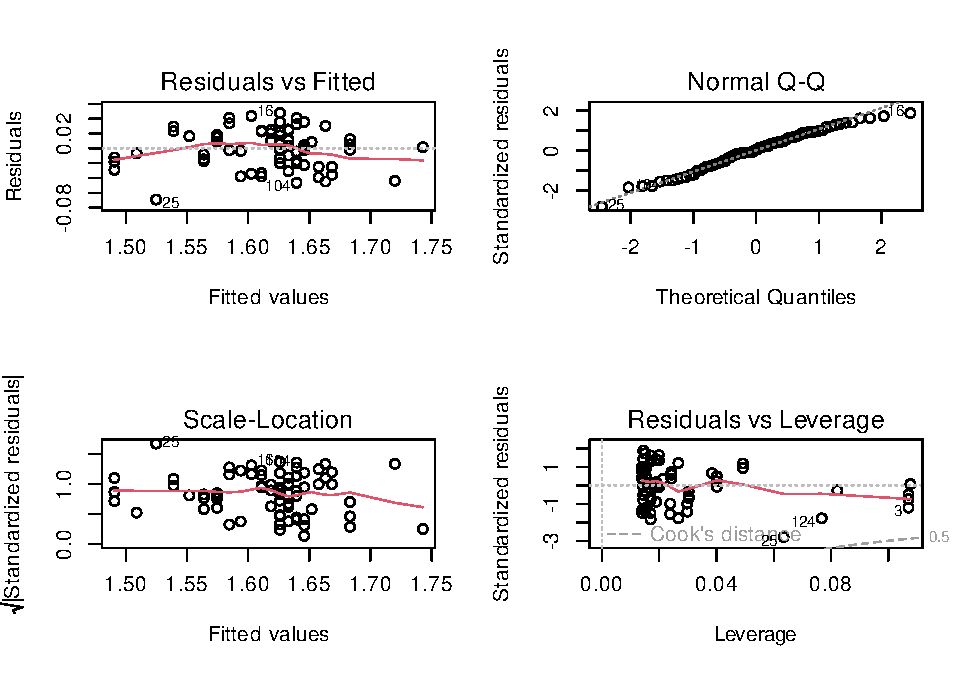
\includegraphics{Labs_BIO4158_files/figure-latex/sturtr-6-1.pdf}

\begin{Shaded}
\begin{Highlighting}[]
\KeywordTok{bptest}\NormalTok{(RegModel}\FloatTok{.3}\NormalTok{)}
\end{Highlighting}
\end{Shaded}

\begin{verbatim}
## 
##  studentized Breusch-Pagan test
## 
## data:  RegModel.3
## BP = 0.3001, df = 1, p-value = 0.5838
\end{verbatim}

\begin{Shaded}
\begin{Highlighting}[]
\KeywordTok{dwtest}\NormalTok{(RegModel}\FloatTok{.3}\NormalTok{)}
\end{Highlighting}
\end{Shaded}

\begin{verbatim}
## 
##  Durbin-Watson test
## 
## data:  RegModel.3
## DW = 2.0171, p-value = 0.5074
## alternative hypothesis: true autocorrelation is greater than 0
\end{verbatim}

\begin{Shaded}
\begin{Highlighting}[]
\KeywordTok{resettest}\NormalTok{(RegModel}\FloatTok{.3}\NormalTok{)}
\end{Highlighting}
\end{Shaded}

\begin{verbatim}
## 
##  RESET test
## 
## data:  RegModel.3
## RESET = 3.407, df1 = 2, df2 = 68, p-value = 0.0389
\end{verbatim}

\begin{Shaded}
\begin{Highlighting}[]
\KeywordTok{shapiro.test}\NormalTok{(}\KeywordTok{residuals}\NormalTok{(RegModel}\FloatTok{.3}\NormalTok{))}
\end{Highlighting}
\end{Shaded}

\begin{verbatim}
## 
##  Shapiro-Wilk normality test
## 
## data:  residuals(RegModel.3)
## W = 0.98318, p-value = 0.4502
\end{verbatim}

No real difference either. Overall, this suggests that the most extreme values do not have undue influence on the results.

\hypertarget{quantifying-effect-size-in-regression-and-power-analysis}{%
\section{Quantifying effect size in regression and power analysis}\label{quantifying-effect-size-in-regression-and-power-analysis}}

Biological interpretation differs from statistical interpretation. Statistically, we conclude that size increase with age (i.e.~the slope is positive and different from 0). But this conclusion alone does not tell if the difference between young and old fish is large. The slope and the scatterplot are more informative than the p-value here. The slope (in log-log space) is 0.34.
This means that for each unit increase of X (\texttt{log10(age)}), there is an increase of 0.34 units of \texttt{log10(fklngth)}. In other words, when age is multiplied by 10, fork length is multiplied by about 2 (10\^{}0.34). Humm, length increases more slowly than age. This slope value (0.34) is an estimate of raw effect size. It measure how much length changes with age.

\hypertarget{power-to-detect-a-given-slope}{%
\subsection{Power to detect a given slope}\label{power-to-detect-a-given-slope}}

You can compute power with G*Power for some slope value that you deem of sufficient magnitude to warrant detection.

\begin{enumerate}
\def\labelenumi{\arabic{enumi}.}
\tightlist
\item
  Go to \textbf{t Tests: Linear bivariate regression: One group, size of slope}.
\item
  Select \textbf{Post hoc: Compute achieved power- given \(\alpha\), sample size,and effect size}
\end{enumerate}

For example, suppose that sturgeon biologists deem that a slope of 0.1 for the relationship between \texttt{log10(fklngth)} and \texttt{log10(age)} is meaningful and you wanted to estimate the power to detect such a slope with a sample of 20 sturgeons. Results from the log-log regression contain most of what you need:

\begin{Shaded}
\begin{Highlighting}[]
\KeywordTok{summary}\NormalTok{(RegModel}\FloatTok{.2}\NormalTok{)}
\end{Highlighting}
\end{Shaded}

\begin{verbatim}
## 
## Call:
## lm(formula = log10(fklngth) ~ log10(age), data = sturgeon.male)
## 
## Residuals:
##       Min        1Q    Median        3Q       Max 
## -0.082794 -0.016837 -0.000719  0.021102  0.087446 
## 
## Coefficients:
##             Estimate Std. Error t value Pr(>|t|)    
## (Intercept)  1.19199    0.02723   43.77   <2e-16 ***
## log10(age)   0.34086    0.02168   15.72   <2e-16 ***
## ---
## Signif. codes:  0 '***' 0.001 '**' 0.01 '*' 0.05 '.' 0.1 ' ' 1
## 
## Residual standard error: 0.03015 on 73 degrees of freedom
##   (5 observations deleted due to missingness)
## Multiple R-squared:  0.772,  Adjusted R-squared:  0.7688 
## F-statistic: 247.1 on 1 and 73 DF,  p-value: < 2.2e-16
\end{verbatim}

Note the Residual standard error value (0.03015). You will need this.
The other thing you need is an estimate of the standard deviation of \texttt{log10(age)}.
R can (of course) compute it. Be careful, the \texttt{sd()} function will return \texttt{NA} if there are missing values. You can get around this by adding \texttt{na.rm=TRUE} as an argument ot the \texttt{sd()} function.

\begin{Shaded}
\begin{Highlighting}[]
\KeywordTok{sd}\NormalTok{(}\KeywordTok{log10}\NormalTok{(sturgeon.male}\OperatorTok{$}\NormalTok{age), }\DataTypeTok{na.rm =} \OtherTok{TRUE}\NormalTok{)}
\end{Highlighting}
\end{Shaded}

\begin{verbatim}
## [1] 0.1616675
\end{verbatim}

You can then enter these values (slope to be detected, sample size, alpha, standard deviation of the independent variable) to calculate another quantity that G*Power needs (standard deviation of y) using the Determine panel. Finally you can calculate Power. The filled panels should look like this

\begin{rmdnote}
Note: The SD of y can't just be taken from the data because if the slope
chanages (e.g.~H1) then this will change the SD of y. SD y needs to be
estimated from the observed scatter around the line and the
hypothesized slope).
\end{rmdnote}

\begin{figure}
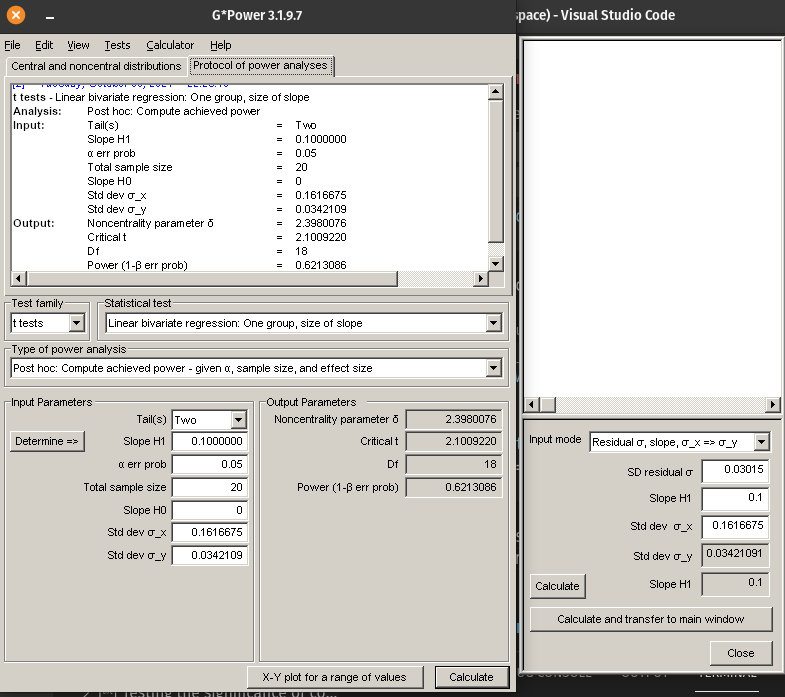
\includegraphics[width=1\linewidth]{images/pow_lm1_en} \caption{Power analysis for age-length in sturgeon with N = 20 and slope = 0.1}\label{fig:lm-pow-fig-1}
\end{figure}

Power to detect a significant slope, if the slope is 0.1, variability of data points around the regression is like in our sample, for a sample of 20 sturgeons, with \(\alpha = 0.05\) is 0.621. Only about 2/3 of samples of that size would detect a significant effect of \texttt{age} on \texttt{fklngth}.

In R, you can do the analysis also but we will use another trick to work with the \texttt{pwr.t.test()} function.
First we, need to estimate the effect size \texttt{d}. IN this case \texttt{d} is estimated as:
\[ d = \frac{b}{s_b\sqrt{n-k-1}} \]
where \(b\) is the slope, \(s_b\) is the standard error on the slope, \(n\) is the number of observations and \(k\) is the number of independent variables (1 for simple liner regression).

SE of the slope is 0.02168. The model was fitted using 75 fishes (n=75). We can then estimate \texttt{d}.
\[ d = \frac{b}{s_b\sqrt{n-k-1}} = \frac{0.1}{0.02168\sqrt{74-1-1}}=0.54\]

We can simply use the \texttt{pwr.t.test()} function to estimate the power.

\begin{Shaded}
\begin{Highlighting}[]
\KeywordTok{library}\NormalTok{(pwr)}

\CommentTok{\# analyse de puissance}
\KeywordTok{pwr.t.test}\NormalTok{(}\DataTypeTok{n =} \DecValTok{20}\NormalTok{, }\DataTypeTok{d =} \FloatTok{0.54}\NormalTok{, }\DataTypeTok{sig.level =} \FloatTok{0.05}\NormalTok{, }\DataTypeTok{type =} \StringTok{"one.sample"}\NormalTok{)}
\end{Highlighting}
\end{Shaded}

\begin{verbatim}
## 
##      One-sample t test power calculation 
## 
##               n = 20
##               d = 0.54
##       sig.level = 0.05
##           power = 0.6299804
##     alternative = two.sided
\end{verbatim}

You can see that the results is really similar but not exactly the same than with G*power which is normal since we did not use the exact same formula to estimate power.

\hypertarget{sample-size-required-to-achieve-desired-power}{%
\subsection{Sample size required to achieve desired power}\label{sample-size-required-to-achieve-desired-power}}

To estimate the sample size required to achieve 99\% power to detect a slope of 0.1 (in log-log space), with alpha=0.05, you simply change the type of analysis:

\begin{figure}
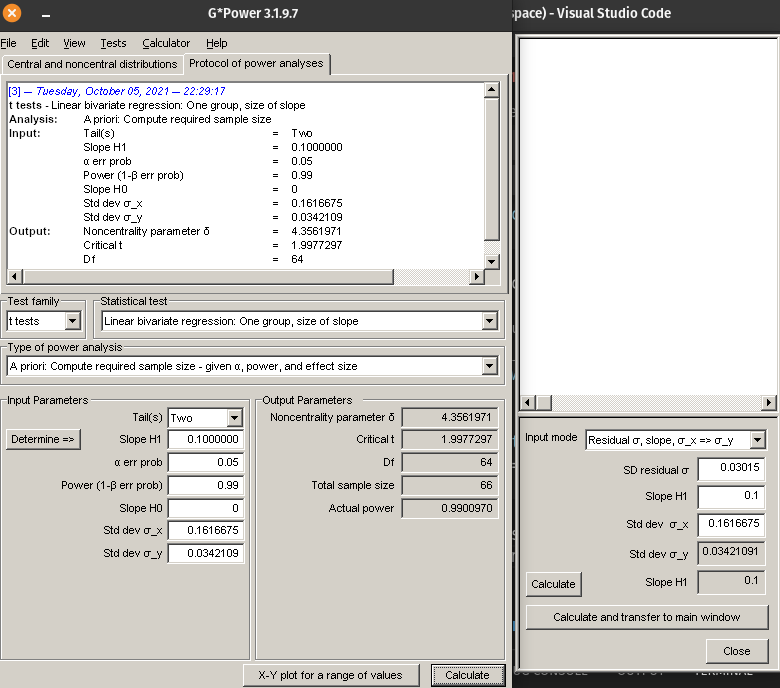
\includegraphics[width=1\linewidth]{images/pow_lm2_en} \caption{A priori power analysis to estimate the sample size needed to have a power of 0.99}\label{fig:lm-pow-fig-2}
\end{figure}

In R you can simply do:

\begin{Shaded}
\begin{Highlighting}[]
\KeywordTok{library}\NormalTok{(pwr)}

\CommentTok{\# analyse de puissance}
\KeywordTok{pwr.t.test}\NormalTok{(}\DataTypeTok{power =} \FloatTok{0.99}\NormalTok{, }\DataTypeTok{d =} \FloatTok{0.54}\NormalTok{, }\DataTypeTok{sig.level =} \FloatTok{0.05}\NormalTok{, }\DataTypeTok{type =} \StringTok{"one.sample"}\NormalTok{)}
\end{Highlighting}
\end{Shaded}

\begin{verbatim}
## 
##      One-sample t test power calculation 
## 
##               n = 64.96719
##               d = 0.54
##       sig.level = 0.05
##           power = 0.99
##     alternative = two.sided
\end{verbatim}

By increasing sample size to 66, with the same assumptions as before, power increases to 99\%.

\hypertarget{bootstrapping-the-simple-linear-regression}{%
\section{Bootstrapping the simple linear regression}\label{bootstrapping-the-simple-linear-regression}}

A non-parametric test for the intercept and slope of a linear regression can be obtained by bootstrapping.

\begin{Shaded}
\begin{Highlighting}[]
\CommentTok{\# load boot}
\KeywordTok{library}\NormalTok{(boot)}
\CommentTok{\# function to obtain regression weights}
\NormalTok{bs \textless{}{-}}\StringTok{ }\ControlFlowTok{function}\NormalTok{(formula, data, indices) \{}
\NormalTok{  d \textless{}{-}}\StringTok{ }\NormalTok{data[indices, ] }\CommentTok{\# allows boot to select sample}
\NormalTok{  fit \textless{}{-}}\StringTok{ }\KeywordTok{lm}\NormalTok{(formula, }\DataTypeTok{data =}\NormalTok{ d)}
  \KeywordTok{return}\NormalTok{(}\KeywordTok{coef}\NormalTok{(fit))}
\NormalTok{\}}
\CommentTok{\# bootstrapping with 1000 replications}
\NormalTok{results \textless{}{-}}\StringTok{ }\KeywordTok{boot}\NormalTok{(}
  \DataTypeTok{data =}\NormalTok{ sturgeon.male,}
  \DataTypeTok{statistic =}\NormalTok{ bs,}
  \DataTypeTok{R =} \DecValTok{1000}\NormalTok{, }\DataTypeTok{formula =} \KeywordTok{log10}\NormalTok{(fklngth) }\OperatorTok{\textasciitilde{}}\StringTok{ }\KeywordTok{log10}\NormalTok{(age)}
\NormalTok{)}
\CommentTok{\# view results}
\NormalTok{results}
\end{Highlighting}
\end{Shaded}

\begin{verbatim}
## 
## ORDINARY NONPARAMETRIC BOOTSTRAP
## 
## 
## Call:
## boot(data = sturgeon.male, statistic = bs, R = 1000, formula = log10(fklngth) ~ 
##     log10(age))
## 
## 
## Bootstrap Statistics :
##      original       bias    std. error
## t1* 1.1919926  0.002516046  0.03236783
## t2* 0.3408557 -0.001825217  0.02577462
\end{verbatim}

For each parameter in the model (here the intercept is labeled \texttt{t1\textbackslash{}*} and the slope of the regression line is labeled \texttt{t2\textbackslash{}*}) , you obtain:

Pour chaque paramètre du modèle (ici l'ordonnée à l'origine est
appelée t1* et la pente de la régression \texttt{t2\textbackslash{}*}), R imprime :

\begin{enumerate}
\def\labelenumi{\arabic{enumi}.}
\tightlist
\item
  \texttt{original} original parameter estimate (on all non-bootstrapped data)
\item
  \texttt{bias} the difference between the mean value of all bootstrap estimates and the original value
\item
  \texttt{std.\ error} standard error of the bootstrap estimate
\end{enumerate}

\begin{Shaded}
\begin{Highlighting}[]
\KeywordTok{par}\NormalTok{(}\DataTypeTok{mfrow =} \KeywordTok{c}\NormalTok{(}\DecValTok{2}\NormalTok{, }\DecValTok{2}\NormalTok{))}
\KeywordTok{plot}\NormalTok{(results, }\DataTypeTok{index =} \DecValTok{1}\NormalTok{) }\CommentTok{\# intercept}
\end{Highlighting}
\end{Shaded}

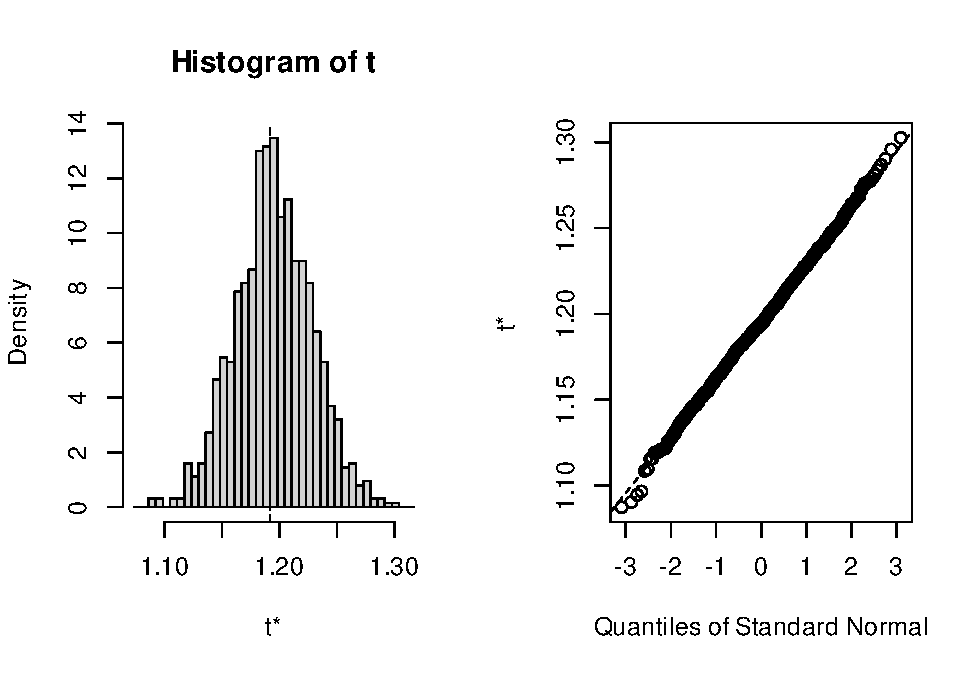
\includegraphics{Labs_BIO4158_files/figure-latex/lm-boot-2-1.pdf}

\begin{Shaded}
\begin{Highlighting}[]
\KeywordTok{plot}\NormalTok{(results, }\DataTypeTok{index =} \DecValTok{2}\NormalTok{) }\CommentTok{\# log10(age)}
\end{Highlighting}
\end{Shaded}

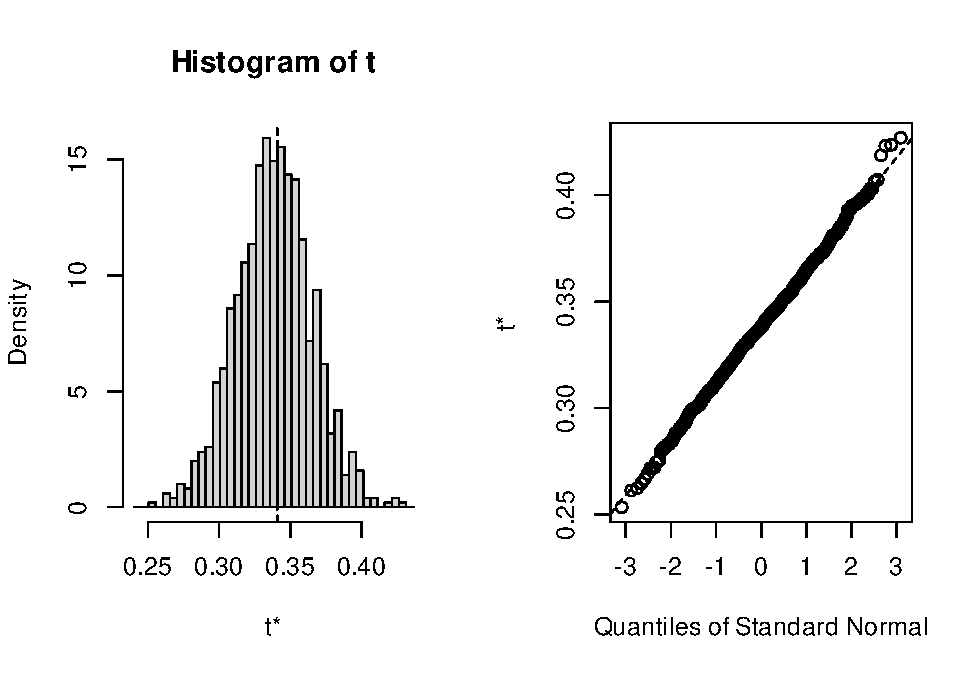
\includegraphics{Labs_BIO4158_files/figure-latex/lm-boot-2-2.pdf}

The distribution of the bootstrapped estimates is rather Gaussian, with only small deviations in the tails (where it counts for confidence intervals\ldots). One could use the standard error of the bootstrap estimates to calculate a symmetrical confidence interval as mean +- t SE. But, given that R can as easily calculate a bias-corrected adjusted (BCa) confidence interval, or one based on the actual distribution, (Percentile) why not have it do it all:

\begin{Shaded}
\begin{Highlighting}[]
\CommentTok{\# interval de confiance pour l\textquotesingle{}ordonnée à l\textquotesingle{}origine}
\KeywordTok{boot.ci}\NormalTok{(results, }\DataTypeTok{type =} \StringTok{"all"}\NormalTok{, }\DataTypeTok{index =} \DecValTok{1}\NormalTok{)}
\end{Highlighting}
\end{Shaded}

\begin{verbatim}
## Warning in boot.ci(results, type = "all", index = 1): bootstrap variances needed
## for studentized intervals
\end{verbatim}

\begin{verbatim}
## BOOTSTRAP CONFIDENCE INTERVAL CALCULATIONS
## Based on 1000 bootstrap replicates
## 
## CALL : 
## boot.ci(boot.out = results, type = "all", index = 1)
## 
## Intervals : 
## Level      Normal              Basic         
## 95%   ( 1.126,  1.253 )   ( 1.122,  1.251 )  
## 
## Level     Percentile            BCa          
## 95%   ( 1.133,  1.262 )   ( 1.123,  1.247 )  
## Calculations and Intervals on Original Scale
## Some BCa intervals may be unstable
\end{verbatim}

\begin{Shaded}
\begin{Highlighting}[]
\CommentTok{\# intervalle de confiance pour la pente}
\KeywordTok{boot.ci}\NormalTok{(results, }\DataTypeTok{type =} \StringTok{"all"}\NormalTok{, }\DataTypeTok{index =} \DecValTok{2}\NormalTok{)}
\end{Highlighting}
\end{Shaded}

\begin{verbatim}
## Warning in boot.ci(results, type = "all", index = 2): bootstrap variances needed
## for studentized intervals
\end{verbatim}

\begin{verbatim}
## BOOTSTRAP CONFIDENCE INTERVAL CALCULATIONS
## Based on 1000 bootstrap replicates
## 
## CALL : 
## boot.ci(boot.out = results, type = "all", index = 2)
## 
## Intervals : 
## Level      Normal              Basic         
## 95%   ( 0.2922,  0.3932 )   ( 0.2926,  0.3953 )  
## 
## Level     Percentile            BCa          
## 95%   ( 0.2864,  0.3891 )   ( 0.2959,  0.3948 )  
## Calculations and Intervals on Original Scale
\end{verbatim}

Here the 4 types of CI that R managed to calculate are essentially the same. Had data been violating more strongly the standard assumptions (normality, homoscedasticity), then the different methods (Normal, Basic, Percentile, and BCa) would have diverged more. In that case, which one is best? BCa has the favor of most, currently.

\hypertarget{two---sample-comparisons}{%
\chapter{Two - sample comparisons}\label{two---sample-comparisons}}

After completing this laboratory exercise, you should be able to:

\begin{itemize}
\tightlist
\item
  Use R to visually examine data.
\item
  Use R to compare the means of two normally distributed samples.
\item
  Use R to compare the means of two non-normally distributed
  samples.
\item
  Use R to compare the means of two paired samples
\end{itemize}

\hypertarget{set-ttest}{%
\section{R packages and data}\label{set-ttest}}

For this la b you need:

\begin{itemize}
\tightlist
\item
  R packages:

  \begin{itemize}
  \tightlist
  \item
    car
  \item
    lmtest
  \item
    boot
  \item
    pwr
  \item
    ggplot2
  \item
    performance
  \end{itemize}
\item
  data:

  \begin{itemize}
  \tightlist
  \item
    sturgeon.csv
  \item
    skulldat\_2020.csv
  \end{itemize}
\end{itemize}

You need to load the packages in R with \texttt{library()} and if need needed install them first with \texttt{install.packages()}
For the data, load them using the \texttt{read.csv()} function.

\hypertarget{visual-examination-of-sample-data}{%
\section{Visual examination of sample data}\label{visual-examination-of-sample-data}}

One of the first steps in any type of data analysis is to visualize your data with plots and summary statistics, to get an idea of underlying distributions, possible outliers, and trends in your data. This often begins with plots of the data, such as histograms, probability plots, and box plots, that allow you to get a feel for whether your data are normally distributed, whether they are correlated one to the other, or whether there are any suspicious looking points that may lead you to go back to the original data file to check for errors.

Suppose we want to test the null hypothesis that the size, as indexed by fork length ( \texttt{fklngth} in file \texttt{sturgeon.csv} - the length, in cm, from the tip of the nose to the base of the fork in the caudal fin), of sturgeon at The Pas and Cumberland House is the same. To begin, we have a look at the underlying distributions of the sample data to get a feel for whether the data are normally distributed in each sample. We will not actually test for normality at this point; the assumption of normality in parametric analyses refers always to the residuals and not the raw data themselves. However, if the raw data are non-normally distributed, then you usually have good reason to suspect that the residuals also will be non-normally distributed.

An excellent way to visually compare a data distribution to a normal distribution is to superimpose a histogram of the data and a normal curve. To do so, we must proceed in two steps:

\begin{enumerate}
\def\labelenumi{\arabic{enumi}.}
\tightlist
\item
  tell R that we want to make a histogram with a density curve superimposed
\item
  tell R that we want this to be done for both locations.
\end{enumerate}

\begin{itemize}
\tightlist
\item
  Using the data file \texttt{sturgeon.csv} , generate histograms for \texttt{fklngth} data at The Pas and Cumberland House.
\end{itemize}

\begin{Shaded}
\begin{Highlighting}[]
\CommentTok{\# use "sturgeon" dataframe to make plot called mygraph}
\CommentTok{\# and define x axis as representing fklngth}
\NormalTok{mygraph \textless{}{-}}\StringTok{ }\KeywordTok{ggplot}\NormalTok{(}
  \DataTypeTok{data =}\NormalTok{ sturgeon,}
  \KeywordTok{aes}\NormalTok{(}\DataTypeTok{x =}\NormalTok{ fklngth)}
\NormalTok{) }\OperatorTok{+}
\StringTok{  }\KeywordTok{xlab}\NormalTok{(}\StringTok{"Fork length (cm)"}\NormalTok{)}
\CommentTok{\# add data to the mygraph ggplot}
\NormalTok{mygraph \textless{}{-}}\StringTok{ }\NormalTok{mygraph }\OperatorTok{+}
\StringTok{  }\KeywordTok{geom\_density}\NormalTok{() }\OperatorTok{+}\StringTok{ }\CommentTok{\# add data density smooth}
\StringTok{  }\KeywordTok{geom\_rug}\NormalTok{() }\OperatorTok{+}\StringTok{ }\CommentTok{\# add rug (bars at the bottom of the plot)}
\StringTok{  }\KeywordTok{geom\_histogram}\NormalTok{( }\CommentTok{\# add black semitransparent histogram}
    \KeywordTok{aes}\NormalTok{(}\DataTypeTok{y =}\NormalTok{ ..density..),}
    \DataTypeTok{color =} \StringTok{"black"}\NormalTok{, }\DataTypeTok{alpha =} \FloatTok{0.3}
\NormalTok{  ) }\OperatorTok{+}
\StringTok{  }\CommentTok{\# add normal curve in red, with mean and sd from fklength}
\StringTok{  }\KeywordTok{stat\_function}\NormalTok{(}
    \DataTypeTok{fun =}\NormalTok{ dnorm,}
    \DataTypeTok{args =} \KeywordTok{list}\NormalTok{(}
      \DataTypeTok{mean =} \KeywordTok{mean}\NormalTok{(sturgeon}\OperatorTok{$}\NormalTok{fklngth),}
      \DataTypeTok{sd =} \KeywordTok{sd}\NormalTok{(sturgeon}\OperatorTok{$}\NormalTok{fklngth)}
\NormalTok{    ),}
    \DataTypeTok{color =} \StringTok{"red"}
\NormalTok{  )}
\CommentTok{\# display graph, by location}
\NormalTok{mygraph }\OperatorTok{+}\StringTok{ }\KeywordTok{facet\_grid}\NormalTok{(. }\OperatorTok{\textasciitilde{}}\StringTok{ }\NormalTok{location)}
\end{Highlighting}
\end{Shaded}

\begin{figure}
\centering
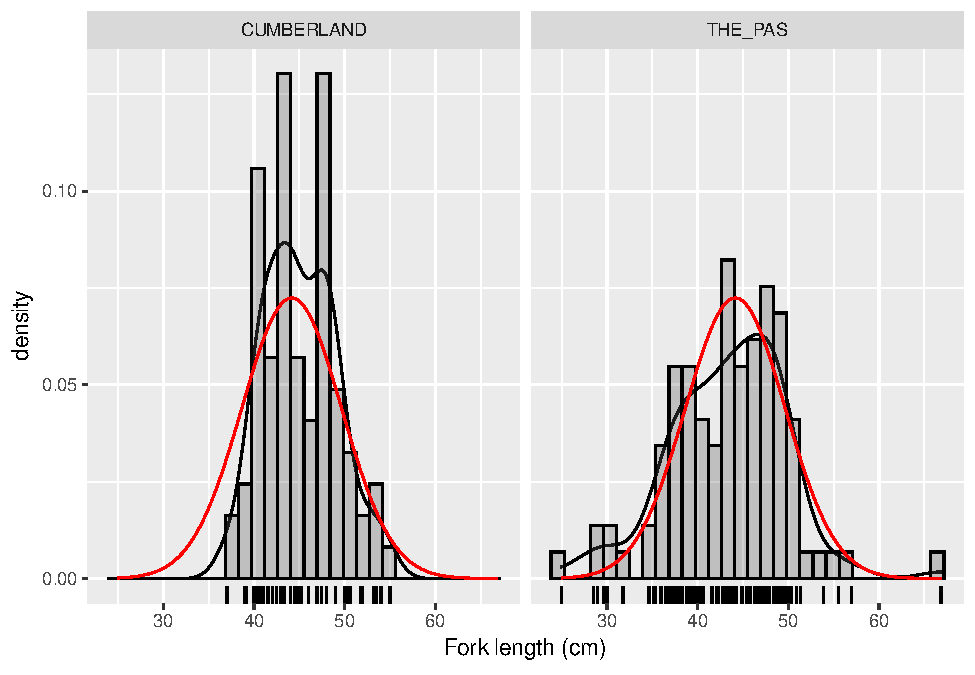
\includegraphics{Labs_BIO4158_files/figure-latex/t-1-1.pdf}
\caption{\label{fig:t-1}Distribution of sturgeon length at 2 locations}
\end{figure}

Based on your visual inspection, are the two samples normally distributed?
Visual inspection of these plots suggests that this variable is approximately normally distributed in each sample.

Since we are interested in finding out if mean fish size differs among the two locations, it is probably also a good idea to generate a graph that compares the two groups of data. A box plot works well for this.

\begin{itemize}
\tightlist
\item
  Generate a box plot of \texttt{fklngth} grouped by \texttt{location} . What do you conclude about differences in size among the two locations?
\end{itemize}

\begin{Shaded}
\begin{Highlighting}[]
\KeywordTok{ggplot}\NormalTok{(}\DataTypeTok{data =}\NormalTok{ sturgeon, }\KeywordTok{aes}\NormalTok{(}
  \DataTypeTok{x =}\NormalTok{ location,}
  \DataTypeTok{y =}\NormalTok{ fklngth}
\NormalTok{)) }\OperatorTok{+}
\StringTok{  }\KeywordTok{geom\_boxplot}\NormalTok{(}\DataTypeTok{notch =} \OtherTok{TRUE}\NormalTok{)}
\end{Highlighting}
\end{Shaded}

\begin{figure}
\centering
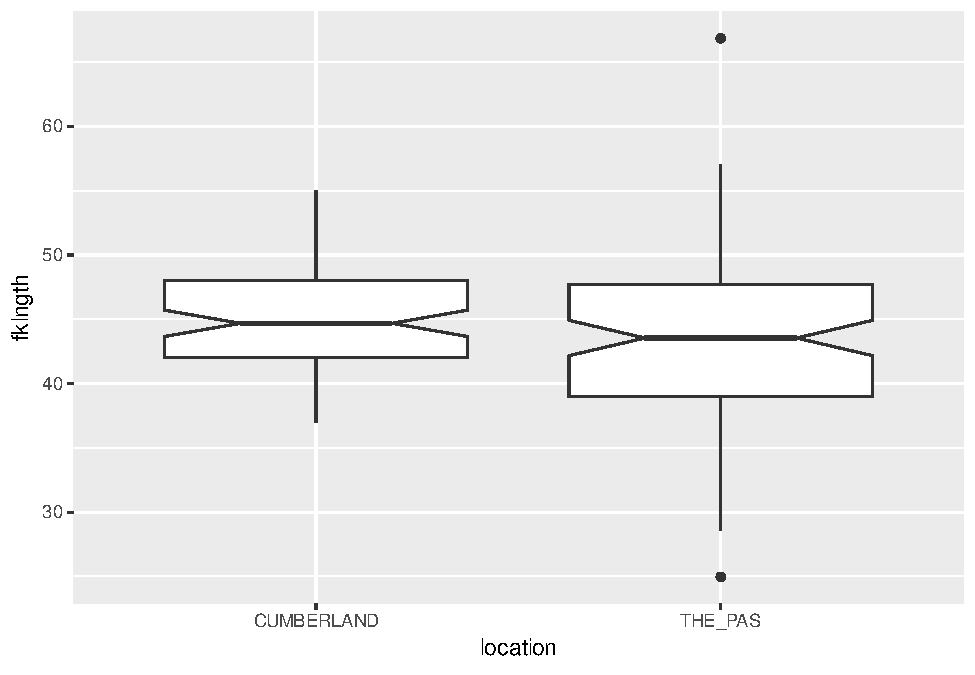
\includegraphics{Labs_BIO4158_files/figure-latex/t-2-1.pdf}
\caption{\label{fig:t-2}Boxplot of sturgeon legnth at 2 locations}
\end{figure}

It would appear as though there are not big differences in fish size among the two locations, although fish size at The Pas looks to be more variable, with a bigger range in size and outliers (defined as values \textgreater{} 1.5 * inter-quartile range) at both ends of the distribution.

\hypertarget{comparing-means-of-two-independent-samples-parametric-and-non-parametric-comparisons}{%
\section{Comparing means of two independent samples: parametric and non-parametric comparisons}\label{comparing-means-of-two-independent-samples-parametric-and-non-parametric-comparisons}}

Test the null hypothesis that the mean fklngth of The Pas and Cumberland House samples are the same. Using 3 different tests:

\begin{enumerate}
\def\labelenumi{\arabic{enumi}.}
\tightlist
\item
  parametric test with equal variances
\item
  parametric test with unequal variances
\item
  non-parametric test
\end{enumerate}

What do you conclude?

\begin{Shaded}
\begin{Highlighting}[]
\CommentTok{\# t{-}test assuming equal variances}
\KeywordTok{t.test}\NormalTok{(}
\NormalTok{  fklngth }\OperatorTok{\textasciitilde{}}\StringTok{ }\NormalTok{location,}
  \DataTypeTok{data =}\NormalTok{ sturgeon,}
  \DataTypeTok{alternative =} \StringTok{"two.sided"}\NormalTok{,}
  \DataTypeTok{var.equal =} \OtherTok{TRUE}
\NormalTok{)}
\end{Highlighting}
\end{Shaded}

\begin{verbatim}
## 
##  Two Sample t-test
## 
## data:  fklngth by location
## t = 2.1359, df = 184, p-value = 0.03401
## alternative hypothesis: true difference in means between group CUMBERLAND and group THE_PAS is not equal to 0
## 95 percent confidence interval:
##  0.1308307 3.2982615
## sample estimates:
## mean in group CUMBERLAND    mean in group THE_PAS 
##                 45.08439                 43.36984
\end{verbatim}

\begin{Shaded}
\begin{Highlighting}[]
\CommentTok{\# t{-}test assuming unequal variances}
\KeywordTok{t.test}\NormalTok{(}
\NormalTok{  fklngth }\OperatorTok{\textasciitilde{}}\StringTok{ }\NormalTok{location,}
  \DataTypeTok{data =}\NormalTok{ sturgeon,}
  \DataTypeTok{alternative =} \StringTok{"two.sided"}\NormalTok{,}
  \DataTypeTok{var.equal =} \OtherTok{FALSE}
\NormalTok{)}
\end{Highlighting}
\end{Shaded}

\begin{verbatim}
## 
##  Welch Two Sample t-test
## 
## data:  fklngth by location
## t = 2.2201, df = 169.8, p-value = 0.02774
## alternative hypothesis: true difference in means between group CUMBERLAND and group THE_PAS is not equal to 0
## 95 percent confidence interval:
##  0.1900117 3.2390804
## sample estimates:
## mean in group CUMBERLAND    mean in group THE_PAS 
##                 45.08439                 43.36984
\end{verbatim}

\begin{Shaded}
\begin{Highlighting}[]
\CommentTok{\# test non paramétrique}
\KeywordTok{wilcox.test}\NormalTok{(}
\NormalTok{  fklngth }\OperatorTok{\textasciitilde{}}\StringTok{ }\NormalTok{location,}
  \DataTypeTok{data =}\NormalTok{ sturgeon,}
  \DataTypeTok{alternative =} \StringTok{"two.sided"}
\NormalTok{)}
\end{Highlighting}
\end{Shaded}

\begin{verbatim}
## 
##  Wilcoxon rank sum test with continuity correction
## 
## data:  fklngth by location
## W = 4973, p-value = 0.06296
## alternative hypothesis: true location shift is not equal to 0
\end{verbatim}

Based on the \emph{t-test}, we would reject the null hypothesis, \emph{i.e.} there is a significant (but not highly significant) difference in mean fork length between the two populations.

Note that using the Wilcoxon rank sum test, we do not reject the null hypothesis. The two different tests therefore give us two different results. The significant difference obtained using the t-test may, at least in part, be due to deviations from normality or homoscedasticity; on the other hand, the non-significant difference obtained using the U -statistic may be due to the fact that for fixed sample size, the power of a non- parametric test is lower than the corresponding parametric test. Given the p values obtained from both tests, and the fact that for samples of this size (84 and 101), the t-test is comparatively robust with respect to non-normality, I would be inclined to reject the null hypothesis. In practice to avoid P-hacking, you should decide which test is appropriate first and then apply and interpret it, or if you decide to do all you should present results of all and interpret accordingly.

Before accepting the results of the parametric t-test and rejecting the null hypothesis that there is no difference in size between the two locations, one should do some sort of assessment to determine if the model fits the assumption of normally distributed residuals and equal variances. Preliminary examination of the raw data suggested the data appeared roughly normal but there might be problems with variances (since the spread of data for The\_Pas was much greater than for Cumberland). We can examine this more closely by looking at the residuals. An easy way to do so, is to fit a linear model and use the residual diagnostic plots:

\begin{Shaded}
\begin{Highlighting}[]
\NormalTok{m1 \textless{}{-}}\StringTok{ }\KeywordTok{lm}\NormalTok{(fklngth }\OperatorTok{\textasciitilde{}}\StringTok{ }\NormalTok{location, }\DataTypeTok{data =}\NormalTok{ sturgeon)}
\KeywordTok{par}\NormalTok{(}\DataTypeTok{mfrow =} \KeywordTok{c}\NormalTok{(}\DecValTok{2}\NormalTok{, }\DecValTok{2}\NormalTok{))}
\KeywordTok{plot}\NormalTok{(m1)}
\end{Highlighting}
\end{Shaded}

\begin{figure}
\centering
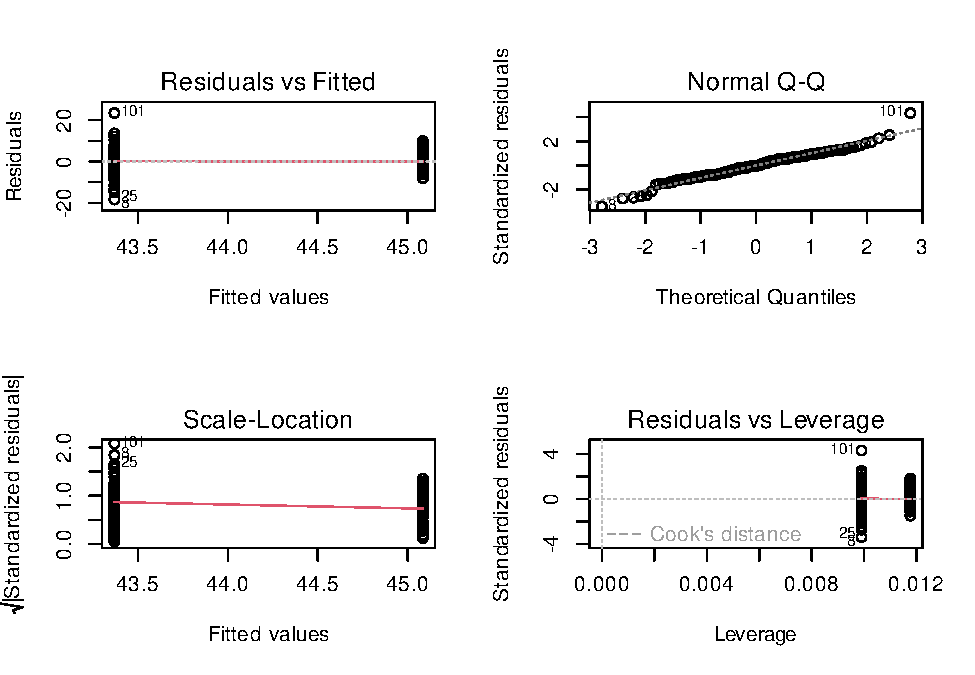
\includegraphics{Labs_BIO4158_files/figure-latex/t-6-1.pdf}
\caption{\label{fig:t-6}Model assumption checks}
\end{figure}

The first plot above shows the spread of the residuals around the estimated values for the two groups and allows us to get a feel for whether there are problems with the assumption of homogeneity of variances. If the variances were equal, the vertical spread of the two clusters of points should be about the same. The above plot shows that the vertical spread of the group with the smaller mean is greater than it is for the larger mean, suggesting again that there are problems with the variances. We can test this formally by examining the mean differences in the absolute value of the residuals.

The second graph above is a normal QQ plot (or probability plot) of the residuals of the model. Note that these generally fall on a straight line, suggesting there is no real problem with normality. We can do a formal test for normality on the residuals using the Shapiro-Wilk test.

\begin{Shaded}
\begin{Highlighting}[]
\KeywordTok{shapiro.test}\NormalTok{(}\KeywordTok{residuals}\NormalTok{(m1))}
\end{Highlighting}
\end{Shaded}

\begin{verbatim}
## 
##  Shapiro-Wilk normality test
## 
## data:  residuals(m1)
## W = 0.97469, p-value = 0.001857
\end{verbatim}

Hummm. The test indicates that the residuals are not normal. But, given that (a) the distribution is not very far (at least visually) from normal, and that (b) the number of observations in each location is reasonably large (i.e.~\textgreater30), we do not need to be overly concerned with this violation of the normality assumption.

How about equality of variance?

\begin{Shaded}
\begin{Highlighting}[]
\KeywordTok{library}\NormalTok{(car)}
\KeywordTok{leveneTest}\NormalTok{(m1)}
\end{Highlighting}
\end{Shaded}

\begin{verbatim}
## Warning in leveneTest.default(y = y, group = group, ...): group coerced to
## factor.
\end{verbatim}

\begin{verbatim}
## Levene's Test for Homogeneity of Variance (center = median)
##        Df F value    Pr(>F)    
## group   1  11.514 0.0008456 ***
##       184                      
## ---
## Signif. codes:  0 '***' 0.001 '**' 0.01 '*' 0.05 '.' 0.1 ' ' 1
\end{verbatim}

\begin{Shaded}
\begin{Highlighting}[]
\KeywordTok{bptest}\NormalTok{(m1)}
\end{Highlighting}
\end{Shaded}

\begin{verbatim}
## 
##  studentized Breusch-Pagan test
## 
## data:  m1
## BP = 8.8015, df = 1, p-value = 0.00301
\end{verbatim}

The above are the results of two tests implemented in R (in the \texttt{car} and \texttt{lmtest} packages 📦 that can be used to test for equal variances in t-tests or linear models involving only discontinuous or categorical independent variables. \textbf{Doing the two of them is overkill}. There is not much to prefer one test over another. Levene test is possibly the
better known. It tests whether the mean of absolute values of the residuals differs among groups. The Breusch-Pagan test has the advantage of being applicable to more linear models (it can deal with regression-type continuous independent variables, at least to some extent). It tests whether the studentized (i.e.~scaled by their sd estimate) squared residuals vary with the independent variables in a linear model. In this case, both indicate that variances are unequal.

On the basis of these results, we conclude that there is evidence (albeit weak) to reject the null hypothesis of no difference in \texttt{fklngth} by \texttt{location}. We have modified the \texttt{t-test} to accommodate unequal variances, and are satisfied that the assumption of normally distributed residuals is sufficiently met. Thus, it appears that \texttt{fklngth} at Cumberland is greater than \texttt{fklngth} at The Pas.

\hypertarget{bootstrap-and-permutation-tests-to-compare-2-means}{%
\section{Bootstrap and permutation tests to compare 2 means}\label{bootstrap-and-permutation-tests-to-compare-2-means}}

\hypertarget{bootstrap}{%
\subsection{Bootstrap}\label{bootstrap}}

Bootstrap and permutation tests can be used to compare means (or other statistics) between pairs of samples. The general idea is simple, and it can be implemented in more ways than I can count. Here, I use existing tools and the fact that a comparison of means can be construed as a test of a linear model. We will be able to use similar code later on when we fit more complex (but fun!) models.

\begin{Shaded}
\begin{Highlighting}[]
\KeywordTok{library}\NormalTok{(boot)}
\end{Highlighting}
\end{Shaded}

The first section defines the function that I called bs that simply extracts coefficients from a fitted model:

\begin{Shaded}
\begin{Highlighting}[]
\CommentTok{\# function to obtain model coefficients for each iteration}
\NormalTok{bs \textless{}{-}}\StringTok{ }\ControlFlowTok{function}\NormalTok{(formula, data, indices) \{}
\NormalTok{  d \textless{}{-}}\StringTok{ }\NormalTok{data[indices, ]}
\NormalTok{  fit \textless{}{-}}\StringTok{ }\KeywordTok{lm}\NormalTok{(formula, }\DataTypeTok{data =}\NormalTok{ d)}
  \KeywordTok{return}\NormalTok{(}\KeywordTok{coef}\NormalTok{(fit))}
\NormalTok{\}}
\end{Highlighting}
\end{Shaded}

The second section with the \texttt{boot()} command is where the real work is done: take data in sturgeon, bootstrap \(R = 1000\) times, each time fit the model \texttt{fklngth} vs \texttt{location}, and keep the values calculated by the \texttt{bs()} function.

\begin{Shaded}
\begin{Highlighting}[]
\CommentTok{\# bootstrapping with 1000 replications}
\NormalTok{results \textless{}{-}}\StringTok{ }\KeywordTok{boot}\NormalTok{(}
  \DataTypeTok{data =}\NormalTok{ sturgeon, }\DataTypeTok{statistic =}\NormalTok{ bs, }\DataTypeTok{R =} \DecValTok{1000}\NormalTok{,}
  \DataTypeTok{formula =}\NormalTok{ fklngth }\OperatorTok{\textasciitilde{}}\StringTok{ }\NormalTok{location}
\NormalTok{)}
\CommentTok{\# view results}
\NormalTok{results}
\end{Highlighting}
\end{Shaded}

\begin{verbatim}
## 
## ORDINARY NONPARAMETRIC BOOTSTRAP
## 
## 
## Call:
## boot(data = sturgeon, statistic = bs, R = 1000, formula = fklngth ~ 
##     location)
## 
## 
## Bootstrap Statistics :
##      original      bias    std. error
## t1* 45.084391 -0.01616052   0.4249350
## t2* -1.714546  0.03934641   0.7715393
\end{verbatim}

So we get the original estimates for the two coefficients in this model: the mean at the first (alphabetical) location, Cumberland, and the difference in means between Cumberland and The Pas ). It is the second parameter, the difference between means, which is of interest here.

\begin{Shaded}
\begin{Highlighting}[]
\KeywordTok{plot}\NormalTok{(results, }\DataTypeTok{index =} \DecValTok{2}\NormalTok{)}
\end{Highlighting}
\end{Shaded}

\begin{figure}
\centering
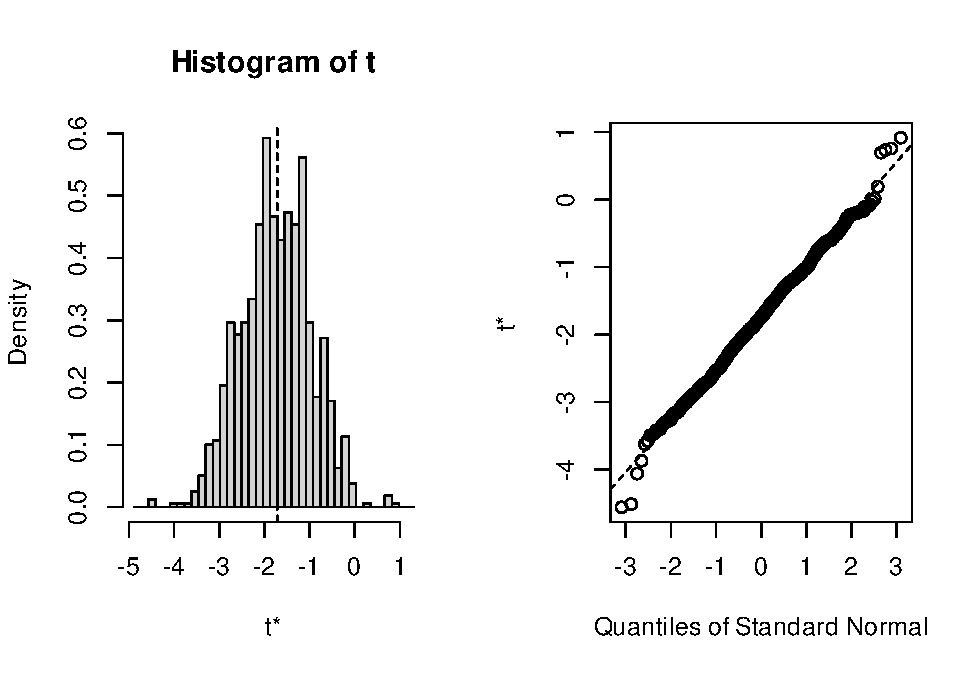
\includegraphics{Labs_BIO4158_files/figure-latex/tb-3-1.pdf}
\caption{\label{fig:tb-3}Distribution of bootstrapped mean difference}
\end{figure}

\begin{Shaded}
\begin{Highlighting}[]
\CommentTok{\# get 95\% confidence intervals}
\KeywordTok{boot.ci}\NormalTok{(results, }\DataTypeTok{type =} \StringTok{"bca"}\NormalTok{, }\DataTypeTok{index =} \DecValTok{2}\NormalTok{)}
\end{Highlighting}
\end{Shaded}

\begin{verbatim}
## BOOTSTRAP CONFIDENCE INTERVAL CALCULATIONS
## Based on 1000 bootstrap replicates
## 
## CALL : 
## boot.ci(boot.out = results, type = "bca", index = 2)
## 
## Intervals : 
## Level       BCa          
## 95%   (-3.261, -0.270 )  
## Calculations and Intervals on Original Scale
\end{verbatim}

The 95\% CI for the difference between the two means does not include 0. Hence, the bootstrap test indicates that the two means are not equals.

\hypertarget{permutation}{%
\subsection{Permutation}\label{permutation}}

Permutation tests for linear models can easily be done using the \texttt{lmPerm} package 📦.

\begin{Shaded}
\begin{Highlighting}[]
\NormalTok{m1Perm \textless{}{-}}\StringTok{ }\KeywordTok{lmp}\NormalTok{(}
\NormalTok{  fklngth }\OperatorTok{\textasciitilde{}}\StringTok{ }\NormalTok{location,}
  \DataTypeTok{data =}\NormalTok{ sturgeon,}
  \DataTypeTok{perm =} \StringTok{"Prob"}
\NormalTok{)}
\end{Highlighting}
\end{Shaded}

\begin{verbatim}
## [1] "Settings:  unique SS "
\end{verbatim}

The \texttt{lmp()} function does all the work for us. Here it is run with the option perm to control the stopping rule used. Option Prob stops the sampling when the estimated standard deviation of the p-value falls below some fraction of the estimated. It is one of many stopping rules that one could use to do permutations on a subset of all the possibilities (because it would take foreeeever to do them all, even on your fast machine).

\begin{Shaded}
\begin{Highlighting}[]
\KeywordTok{summary}\NormalTok{(m1Perm)}
\end{Highlighting}
\end{Shaded}

\begin{verbatim}
## 
## Call:
## lmp(formula = fklngth ~ location, data = sturgeon, perm = "Prob")
## 
## Residuals:
##       Min        1Q    Median        3Q       Max 
## -18.40921  -3.75370  -0.08439   3.76598  23.48055 
## 
## Coefficients:
##           Estimate Iter Pr(Prob)  
## location1   0.8573 3818   0.0257 *
## ---
## Signif. codes:  0 '***' 0.001 '**' 0.01 '*' 0.05 '.' 0.1 ' ' 1
## 
## Residual standard error: 5.454 on 184 degrees of freedom
## Multiple R-Squared: 0.02419, Adjusted R-squared: 0.01889 
## F-statistic: 4.562 on 1 and 184 DF,  p-value: 0.03401
\end{verbatim}

\begin{enumerate}
\def\labelenumi{\arabic{enumi}.}
\tightlist
\item
  \texttt{Iter} coefficient: the Prob stopping rule stopped after 3818 iterations. Note that this number will vary each time you run this snippet of code. These are random permutation results, so expect variability.
\item
  \texttt{Pr(Prob)} coefficient: The estimated probability associated to H0 is 0.0257 . The observed difference in fklngth between the two locations was larger than the permuted differences in about (1 - 0.0257= about 97.4\%) of the 3818 cases. Mind you, 3818 permutations is not a large number, so small p values can't be expected to be very precise. If it is critical that you get more precise p values, more permutations would be needed. Two parameters can be tweaked: maxIter, the maximum number of iterations (default=5000), and Ca, that stops iterations when estimated standard error of the estimated p is less than Ca*p.~Default 0.1.
\item
  \texttt{F-statistic}: The rest is the standard output for the model fitted to the data, with the standard parametric test. Here the p-value, assuming all assumptions are met, is 0.034.
\end{enumerate}

\hypertarget{comparing-the-means-of-paired-samples}{%
\section{Comparing the means of paired samples}\label{comparing-the-means-of-paired-samples}}

In some experimental designs, individuals are measured twice: common examples are the measurement of the same individual at two different times during development, or of the same individual subjected to two different experimental treatments. In these cases, the two samples are not independent (they include the same individuals), and a paired comparison must be made.

The file \texttt{skulldat\_2020.csv} shows measurements of lower face width of 15 North American girls measured at age 5 and again at age 6 years (data from Newman and Meredith, 1956).

\begin{itemize}
\tightlist
\item
  Let's first run a standard t-test comparing the face width at age 5 and 6, not taking into account that the data are not independent and that they are consecutive measurements on the same individuals.
\end{itemize}

\begin{Shaded}
\begin{Highlighting}[]
\NormalTok{skull \textless{}{-}}\StringTok{ }\KeywordTok{read.csv}\NormalTok{(}\StringTok{"data/skulldat\_2020.csv"}\NormalTok{)}
\KeywordTok{t.test}\NormalTok{(width }\OperatorTok{\textasciitilde{}}\StringTok{ }\NormalTok{age,}
  \DataTypeTok{data =}\NormalTok{ skull,}
  \DataTypeTok{alternative =} \StringTok{"two.sided"}\NormalTok{,}
  \DataTypeTok{paired =} \OtherTok{FALSE}
\NormalTok{)}
\end{Highlighting}
\end{Shaded}

\begin{verbatim}
## 
##  Welch Two Sample t-test
## 
## data:  width by age
## t = -1.7812, df = 27.93, p-value = 0.08576
## alternative hypothesis: true difference in means between group 5 and group 6 is not equal to 0
## 95 percent confidence interval:
##  -0.43002624  0.03002624
## sample estimates:
## mean in group 5 mean in group 6 
##        7.461333        7.661333
\end{verbatim}

So far, we specified the t-test using a \texttt{formula} notation as \texttt{y\ \textasciitilde{}\ x} where \texttt{y} is the variable for which we want to compare the means and \texttt{x} is a variable defining the groups. This works really well when the samples are not paired and when the data is presented in a \emph{long} format. For example the\texttt{skull} data is presented in a long format and contains 3 variables:

\begin{itemize}
\tightlist
\item
  \texttt{width}: head width for each observations
\item
  \texttt{age}: age at measurement 5 or 6
\item
  \texttt{id}: person identity
\end{itemize}

\begin{Shaded}
\begin{Highlighting}[]
\KeywordTok{head}\NormalTok{(skull)}
\end{Highlighting}
\end{Shaded}

\begin{verbatim}
##   width age id
## 1  7.33   5  1
## 2  7.53   6  1
## 3  7.49   5  2
## 4  7.70   6  2
## 5  7.27   5  3
## 6  7.46   6  3
\end{verbatim}

When data are paired, we need to indicate how they are paired. In the \texttt{skull}data, samples are paired by an individual identity, \texttt{id}, with mearurement taken at different ages. However, the function \texttt{t.test} does not cope well with this data structure. We need to transpose the data from a \emph{long} to a \emph{wide} format where we have a column per group, with the data of a given individual on the same line. Here is how we can do it.

\begin{Shaded}
\begin{Highlighting}[]
\NormalTok{skull\_w \textless{}{-}}\StringTok{ }\KeywordTok{data.frame}\NormalTok{(}\DataTypeTok{id =} \KeywordTok{unique}\NormalTok{(skull}\OperatorTok{$}\NormalTok{id))}
\NormalTok{skull\_w}\OperatorTok{$}\NormalTok{width5 \textless{}{-}}\StringTok{ }\NormalTok{skull}\OperatorTok{$}\NormalTok{width[}\KeywordTok{match}\NormalTok{(skull\_w}\OperatorTok{$}\NormalTok{id, skull}\OperatorTok{$}\NormalTok{id) }\OperatorTok{\&}\StringTok{ }\NormalTok{skull}\OperatorTok{$}\NormalTok{age }\OperatorTok{==}\StringTok{ }\DecValTok{5}\NormalTok{]}
\NormalTok{skull\_w}\OperatorTok{$}\NormalTok{width6 \textless{}{-}}\StringTok{ }\NormalTok{skull}\OperatorTok{$}\NormalTok{width[}\KeywordTok{match}\NormalTok{(skull\_w}\OperatorTok{$}\NormalTok{id, skull}\OperatorTok{$}\NormalTok{id) }\OperatorTok{\&}\StringTok{ }\NormalTok{skull}\OperatorTok{$}\NormalTok{age }\OperatorTok{==}\StringTok{ }\DecValTok{6}\NormalTok{]}
\KeywordTok{head}\NormalTok{(skull\_w)}
\end{Highlighting}
\end{Shaded}

\begin{verbatim}
##   id width5 width6
## 1  1   7.33   7.53
## 2  2   7.49   7.70
## 3  3   7.27   7.46
## 4  4   7.93   8.21
## 5  5   7.56   7.81
## 6  6   7.81   8.01
\end{verbatim}

Now, let's run the appropriate paired t-test. What do you conclude?
Compare this with the previous result and explain any differences.

\begin{Shaded}
\begin{Highlighting}[]
\KeywordTok{t.test}\NormalTok{(skull\_w}\OperatorTok{$}\NormalTok{width5, skull\_w}\OperatorTok{$}\NormalTok{width6,}
  \DataTypeTok{alternative =} \StringTok{"two.sided"}\NormalTok{,}
  \DataTypeTok{paired =} \OtherTok{TRUE}
\NormalTok{)}
\end{Highlighting}
\end{Shaded}

\begin{verbatim}
## 
##  Paired t-test
## 
## data:  skull_w$width5 and skull_w$width6
## t = -19.72, df = 14, p-value = 1.301e-11
## alternative hypothesis: true difference in means is not equal to 0
## 95 percent confidence interval:
##  -0.2217521 -0.1782479
## sample estimates:
## mean of the differences 
##                    -0.2
\end{verbatim}

The first analysis above assumes that the two samples of girls at age 5 and 6 are independent samples, whereas the second analysis assumes that the same girl is measured twice, once at age 5 and once at age 6 years.

Note that in the former case, we accept the null based on \(p = 0.05\), but in the latter we reject the null. In other words, the appropriate (paired sample) test shows a very significant effect of age, whereas the inappropriate one does not. The reason is because there is a strong correlation between face width at age 5 and face width at age 6:

\begin{Shaded}
\begin{Highlighting}[]
\NormalTok{graphskull \textless{}{-}}\StringTok{ }\KeywordTok{ggplot}\NormalTok{(}\DataTypeTok{data =}\NormalTok{ skull\_w, }\KeywordTok{aes}\NormalTok{(}\DataTypeTok{x =}\NormalTok{ width5, }\DataTypeTok{y =}\NormalTok{ width6)) }\OperatorTok{+}
\StringTok{  }\KeywordTok{geom\_point}\NormalTok{() }\OperatorTok{+}
\StringTok{  }\KeywordTok{labs}\NormalTok{(}\DataTypeTok{x =} \StringTok{"Skull width at age 5"}\NormalTok{, }\DataTypeTok{y =} \StringTok{"Skull width at age 6"}\NormalTok{) }\OperatorTok{+}
\StringTok{  }\KeywordTok{geom\_smooth}\NormalTok{() }\OperatorTok{+}
\StringTok{  }\KeywordTok{scale\_fill\_continuous}\NormalTok{(}\DataTypeTok{low =} \StringTok{"lavenderblush"}\NormalTok{, }\DataTypeTok{high =} \StringTok{"red"}\NormalTok{)}
\NormalTok{graphskull}
\end{Highlighting}
\end{Shaded}

\begin{verbatim}
## `geom_smooth()` using method = 'loess' and formula 'y ~ x'
\end{verbatim}

\begin{figure}
\centering
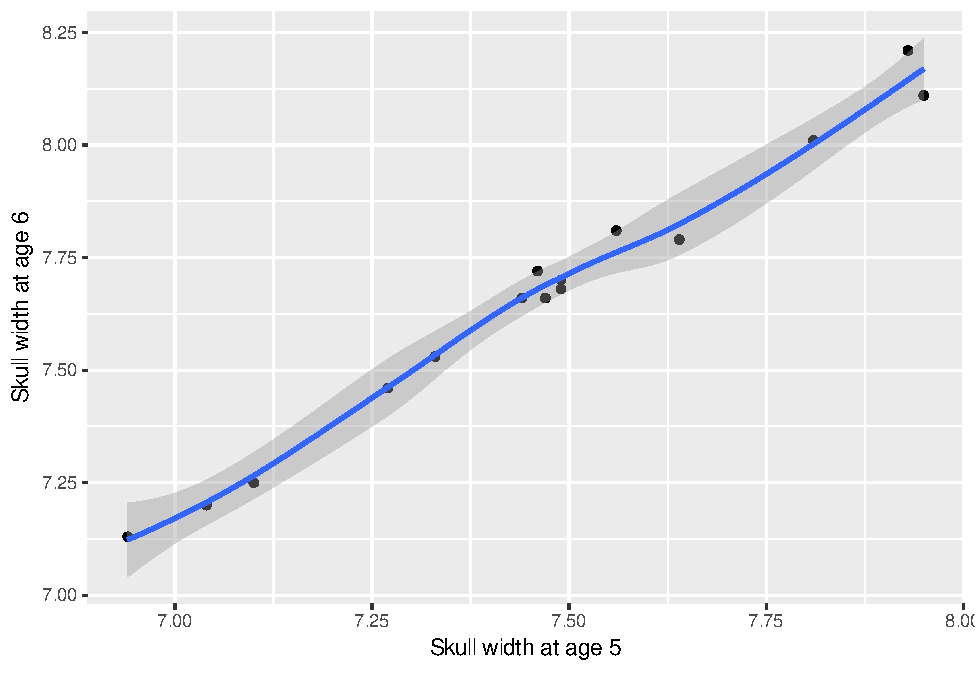
\includegraphics{Labs_BIO4158_files/figure-latex/tpaired-3-1.pdf}
\caption{\label{fig:tpaired-3}Relation between head width at age 5 and 6}
\end{figure}

With \emph{r} = 0.9930841. In the presence of correlation, the standard error of the pairwise difference in face width at age 5 and 6 is much smaller than the standard error of the difference between the mean face width at age 5 and 6. Thus, the associated t-statistic will be much larger for a paired sample test, \emph{i.e.} the power of the test is much greater, and the p values are smaller.

\begin{itemize}
\tightlist
\item
  Repeat the above procedure with the nonparametric alternative, the Wilcoxon signed-rank test. What do you conclude?
\end{itemize}

\begin{Shaded}
\begin{Highlighting}[]
\KeywordTok{wilcox.test}\NormalTok{(skull\_w}\OperatorTok{$}\NormalTok{width5, skull\_w}\OperatorTok{$}\NormalTok{width6,}
  \DataTypeTok{alternative =} \StringTok{"two.sided"}\NormalTok{,}
  \DataTypeTok{paired =} \OtherTok{TRUE}
\NormalTok{)}
\end{Highlighting}
\end{Shaded}

\begin{verbatim}
## Warning in wilcox.test.default(skull_w$width5, skull_w$width6, alternative =
## "two.sided", : cannot compute exact p-value with ties
\end{verbatim}

\begin{verbatim}
## 
##  Wilcoxon signed rank test with continuity correction
## 
## data:  skull_w$width5 and skull_w$width6
## V = 0, p-value = 0.0007193
## alternative hypothesis: true location shift is not equal to 0
\end{verbatim}

So, we reach the same conclusion as we did using the paired sample t- test and conclude there are significant differences in skull sizes of girls aged 5 and 6 (what a surprise!).

But, wait a minute. We have used two-tailed tests here. But, given what we know about how children grow, a one-tail hypothesis would be preferable. This can be done by changing the alternative option. One uses the alternative hypothesis to decide if it is ``less'' or greater". Here, we expect that if there is an effect (i.e the alternative hypothesis), width5 will be less than width6

\begin{Shaded}
\begin{Highlighting}[]
\KeywordTok{t.test}\NormalTok{(skull\_w}\OperatorTok{$}\NormalTok{width5, skull\_w}\OperatorTok{$}\NormalTok{width6,}
  \DataTypeTok{alternative =} \StringTok{"less"}\NormalTok{,}
  \DataTypeTok{paired =} \OtherTok{TRUE}
\NormalTok{)}
\end{Highlighting}
\end{Shaded}

\begin{verbatim}
## 
##  Paired t-test
## 
## data:  skull_w$width5 and skull_w$width6
## t = -19.72, df = 14, p-value = 6.507e-12
## alternative hypothesis: true difference in means is less than 0
## 95 percent confidence interval:
##        -Inf -0.1821371
## sample estimates:
## mean of the differences 
##                    -0.2
\end{verbatim}

\begin{Shaded}
\begin{Highlighting}[]
\KeywordTok{wilcox.test}\NormalTok{(skull\_w}\OperatorTok{$}\NormalTok{width5, skull\_w}\OperatorTok{$}\NormalTok{width6,}
  \DataTypeTok{alternative =} \StringTok{"less"}\NormalTok{,}
  \DataTypeTok{paired =} \OtherTok{TRUE}
\NormalTok{)}
\end{Highlighting}
\end{Shaded}

\begin{verbatim}
## Warning in wilcox.test.default(skull_w$width5, skull_w$width6, alternative =
## "less", : cannot compute exact p-value with ties
\end{verbatim}

\begin{verbatim}
## 
##  Wilcoxon signed rank test with continuity correction
## 
## data:  skull_w$width5 and skull_w$width6
## V = 0, p-value = 0.0003597
## alternative hypothesis: true location shift is less than 0
\end{verbatim}

\begin{rmdwarning}
Note that instead of rerunning the t-test specifying a one-tailed test, you can:

\begin{itemize}
\tightlist
\item
  if the sign of the estimate goes in the same direction as the alternative hypothesis, simply divide by 2 the probability you obtain with the two-tailed test
\item
  if not the sign of the estimate is in the opposite direction of the alternative hypothesis, use \(1 - p/2\)
  \end{rmdwarning}
\end{itemize}

\hypertarget{ruxe9fuxe9rences}{%
\section{Références}\label{ruxe9fuxe9rences}}

Bumpus, H.C. (1898) The elimination of the unfit as illustrated by the introduced sparrow, Passer domesticus. Biological Lectures, Woods Hole Biology Laboratory, Woods Hole, 11 th Lecture: 209 - 226.

Newman, K.J. and H.V. Meredith. (1956) Individual growth in skele- tal bigonial diameter during the childhood period from 5 to 11 years of age. Amer. J. Anat. 99: 157 - 187.

\hypertarget{one-way-anova}{%
\chapter{One-way ANOVA}\label{one-way-anova}}

After completing this laboratory exercise, you should be able to:

\begin{itemize}
\tightlist
\item
  Use R to do a one-way parametric ANOVA with multiple comparisons
\item
  Use R to test the validity of the parametric ANOVA assumptions
\item
  Use R to perform a one-way non-parametric ANOVA
\item
  Use R to transform your data so that the assumptions of parametric ANOVA are met.
\end{itemize}

\hypertarget{set-ano}{%
\section{R packages and data}\label{set-ano}}

For this lab you need:

\begin{itemize}
\tightlist
\item
  R packages:

  \begin{itemize}
  \tightlist
  \item
    ggplot2
  \item
    multcomp
  \item
    car
  \end{itemize}
\item
  data

  \begin{itemize}
  \tightlist
  \item
    dam10dat.csv
  \end{itemize}
\end{itemize}

\begin{Shaded}
\begin{Highlighting}[]
\KeywordTok{library}\NormalTok{(ggplot2)}
\KeywordTok{library}\NormalTok{(car)}
\KeywordTok{library}\NormalTok{(multcomp)}
\end{Highlighting}
\end{Shaded}

\hypertarget{one-way-anova-with-multiple-comparisons}{%
\section{One-way ANOVA with multiple comparisons}\label{one-way-anova-with-multiple-comparisons}}

The one-way ANOVA is the multi-group analog of the \emph{t}-test, which is used to compare two groups/levels. It makes essentially the same assumptions, and in the case of two groups/levels, is in fact mathematically equivalent to the \emph{t}-test.

In 1960-1962, the Grand Rapids Dam was built on the Saskatchewan River upstream of Cumberland House. There are anecdotal reports that during dam construction, a number of large sturgeon were stranded and died in shallow pools. Surveys of sturgeon were carried out in 1954, 1958, 1965 and 1966 with fork length (\texttt{fklngth}) and round weight (\texttt{rdwght}) being recorded (not necessarily both measurements for each individual). These data are in the data file \texttt{Dam10dat.csv}.

\hypertarget{visualiser-les-donnuxe9es}{%
\subsection{Visualiser les données}\label{visualiser-les-donnuxe9es}}

\begin{itemize}
\tightlist
\item
  Using \texttt{Dam10dat.csv}, you must first change the data type of the
  numerical variable year , so that R recognizes that we wish to treat this
  variable as a factor variable and not a continuous variable.
\end{itemize}

\begin{verbatim}
## 'data.frame':    118 obs. of  21 variables:
##  $ year    : Factor w/ 4 levels "1954","1958",..: 1 1 1 1 1 1 1 1 1 1 ...
##  $ fklngth : num  45 50 39 46 54.5 49 42.5 49 56 54 ...
##  $ totlngth: num  49 NA 43 50.5 NA 51.7 45.5 52 60.2 58.5 ...
##  $ drlngth : logi  NA NA NA NA NA NA ...
##  $ drwght  : num  16 20.5 10 17.5 19.7 21.3 9.5 23.7 31 27.3 ...
##  $ rdwght  : num  24.5 33 15.5 28.5 32.5 35.5 15.3 40.5 51.5 43 ...
##  $ sex     : int  1 1 1 2 1 2 1 1 1 1 ...
##  $ age     : int  24 33 17 31 37 44 23 34 33 47 ...
##  $ lfkl    : num  1.65 1.7 1.59 1.66 1.74 ...
##  $ ltotl   : num  1.69 NA 1.63 1.7 NA ...
##  $ ldrl    : logi  NA NA NA NA NA NA ...
##  $ ldrwght : num  1.2 1.31 1 1.24 1.29 ...
##  $ lrdwght : num  1.39 1.52 1.19 1.45 1.51 ...
##  $ lage    : num  1.38 1.52 1.23 1.49 1.57 ...
##  $ rage    : int  4 6 3 6 7 7 4 6 6 7 ...
##  $ ryear   : int  1954 1954 1954 1954 1954 1954 1954 1954 1954 1954 ...
##  $ ryear2  : int  1958 1958 1958 1958 1958 1958 1958 1958 1958 1958 ...
##  $ ryear3  : int  1966 1966 1966 1966 1966 1966 1966 1966 1966 1966 ...
##  $ location: int  1 1 1 1 1 1 1 1 1 1 ...
##  $ girth   : logi  NA NA NA NA NA NA ...
##  $ lgirth  : logi  NA NA NA NA NA NA ...
\end{verbatim}

\begin{itemize}
\tightlist
\item
  Next, have a look at the fklngth data, just as we did in the last lab for t-tests. Create a histogram with density line grouped by year to get a feel for what's happening with your data and a boxplot of length per year. What can you say about these data?
\end{itemize}

\begin{figure}
\centering
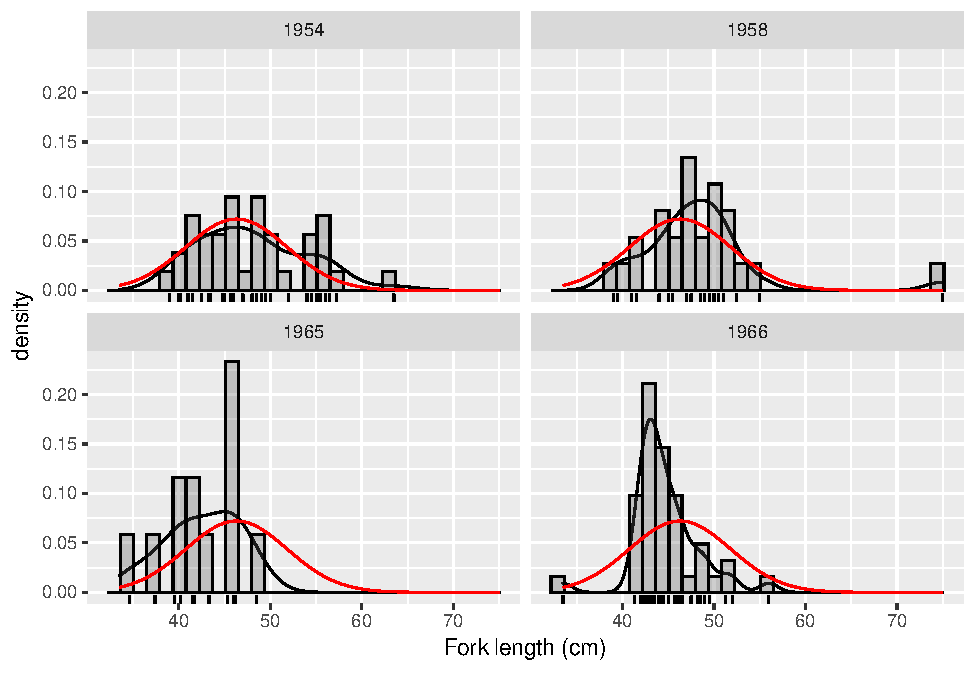
\includegraphics{Labs_BIO4158_files/figure-latex/ano-2-1.pdf}
\caption{\label{fig:ano-2}Distribution of sturgeon length per year}
\end{figure}

\begin{figure}
\centering
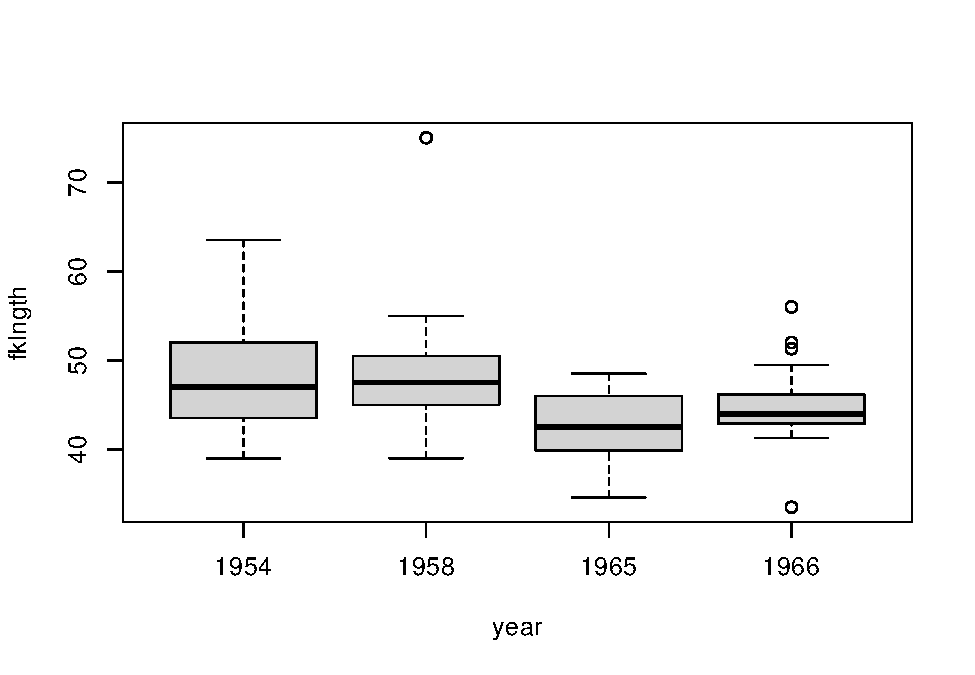
\includegraphics{Labs_BIO4158_files/figure-latex/unnamed-chunk-38-1.pdf}
\caption{\label{fig:unnamed-chunk-38}Boxplot of sturgeon length per year}
\end{figure}

It appears as though there may have been a small drop in \texttt{fklngth} after the construction of the dam, but the data are variable and the effects are not clear. There might also be some problems with normality in the 1954 and 1966 samples, and it looks as though there are outliers in the 1958 and 1966 samples. Let's proceed with testing the assumptions of the ANOVA by running the analysis and looking at the residuals.

\hypertarget{testing-the-assumptions-of-a-parametric-anova}{%
\subsection{Testing the assumptions of a parametric ANOVA}\label{testing-the-assumptions-of-a-parametric-anova}}

Parametric one-way ANOVAs have three major assumptions:

\begin{enumerate}
\def\labelenumi{\arabic{enumi}.}
\tightlist
\item
  the residuals are normally distributed
\item
  the error variance is the same for all groups (homoscedasticity)
\item
  the residuals are independent.
\end{enumerate}

These assumptions must be tested before we can accept the results of any parametric ANOVA.

\begin{itemize}
\tightlist
\item
  Carry out a one-way ANOVA on fklngth by year and produce the residual diagnostic plots
\end{itemize}

\begin{Shaded}
\begin{Highlighting}[]
\CommentTok{\# Fit anova model and plot residual diagnostics}
\NormalTok{anova.model1 \textless{}{-}}\StringTok{ }\KeywordTok{lm}\NormalTok{(fklngth }\OperatorTok{\textasciitilde{}}\StringTok{ }\NormalTok{year, }\DataTypeTok{data =}\NormalTok{ dam10dat)}
\KeywordTok{par}\NormalTok{(}\DataTypeTok{mfrow =} \KeywordTok{c}\NormalTok{(}\DecValTok{2}\NormalTok{, }\DecValTok{2}\NormalTok{))}
\KeywordTok{plot}\NormalTok{(anova.model1)}
\end{Highlighting}
\end{Shaded}

\begin{figure}
\centering
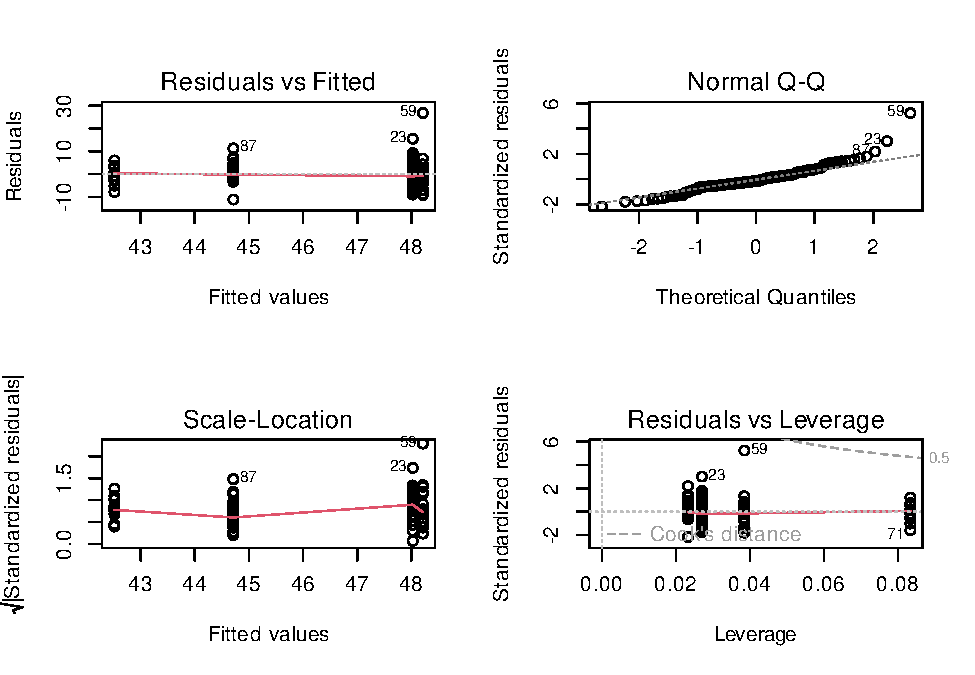
\includegraphics{Labs_BIO4158_files/figure-latex/ano-3-1.pdf}
\caption{\label{fig:ano-3}Diagnostic plots for a one-way ANOVA}
\end{figure}

\begin{rmdwarning}
Double check that the independent variable is a \textbf{factor}. If the dependent variable is a \textbf{character}, then you will obtain only 3 graphs and an error message like:

`hat values (leverages) are all = 0.1

and there are no factor predictors; no plot no. 5`
\end{rmdwarning}

D'après les graphiques, on peut douter de la normalité et de l'homogénéité des variances. Judging from the plots, it looks as though there may be problems with both normality and variance heterogeneity. Note that there is one point (case 59) with large expected values and a large residual that appear to lie well off the line: this is the outlier we noted earlier. This point might be expected to inflate the variance for the group it belongs to. Formal tests may also provide some insight as to whether we should be concerned about normality and variance heterogeneity.

\begin{itemize}
\tightlist
\item
  Perform a normality test on the residuals from the ANOVA.
\end{itemize}

\begin{Shaded}
\begin{Highlighting}[]
\KeywordTok{shapiro.test}\NormalTok{(}\KeywordTok{residuals}\NormalTok{(anova.model1))}
\end{Highlighting}
\end{Shaded}

\begin{verbatim}
## 
##  Shapiro-Wilk normality test
## 
## data:  residuals(anova.model1)
## W = 0.91571, p-value = 1.63e-06
\end{verbatim}

This test confirms our suspicions from the probability plot: the residuals are not normally distributed. Recall, however, that the power here is high, so only small deviations from normality are required to reject the null.

\begin{itemize}
\tightlist
\item
  Next, test for homoscedasticity:
\end{itemize}

\begin{Shaded}
\begin{Highlighting}[]
\KeywordTok{leveneTest}\NormalTok{(fklngth }\OperatorTok{\textasciitilde{}}\StringTok{ }\NormalTok{year, }\DataTypeTok{data =}\NormalTok{ dam10dat)}
\end{Highlighting}
\end{Shaded}

\begin{verbatim}
## Levene's Test for Homogeneity of Variance (center = median)
##        Df F value  Pr(>F)  
## group   3  2.8159 0.04234 *
##       114                  
## ---
## Signif. codes:  0 '***' 0.001 '**' 0.01 '*' 0.05 '.' 0.1 ' ' 1
\end{verbatim}

The probability value tells you that you can reject the null hypothesis that there is no difference in variances among years. Thus, we conclude there is evidence that the variances in the groups are not equal.

\hypertarget{performing-the-anova}{%
\subsection{Performing the ANOVA}\label{performing-the-anova}}

Let's look at the results of the ANOVA, assuming for the moment that assumptions are met well enough.

\begin{Shaded}
\begin{Highlighting}[]
\KeywordTok{summary}\NormalTok{(anova.model1)}
\end{Highlighting}
\end{Shaded}

\begin{verbatim}
## 
## Call:
## lm(formula = fklngth ~ year, data = dam10dat)
## 
## Residuals:
##      Min       1Q   Median       3Q      Max 
## -11.2116  -2.6866  -0.7116   2.2103  26.7885 
## 
## Coefficients:
##             Estimate Std. Error t value Pr(>|t|)    
## (Intercept)  48.0243     0.8566  56.061  < 2e-16 ***
## year1958      0.1872     1.3335   0.140  0.88859    
## year1965     -5.5077     1.7310  -3.182  0.00189 ** 
## year1966     -3.3127     1.1684  -2.835  0.00542 ** 
## ---
## Signif. codes:  0 '***' 0.001 '**' 0.01 '*' 0.05 '.' 0.1 ' ' 1
## 
## Residual standard error: 5.211 on 114 degrees of freedom
## Multiple R-squared:  0.1355, Adjusted R-squared:  0.1128 
## F-statistic: 5.957 on 3 and 114 DF,  p-value: 0.0008246
\end{verbatim}

\begin{itemize}
\tightlist
\item
  \emph{Coefficients: Estimates} Note the 4 coefficients printed. They can be used to obtain the predicted values for the model (i.e.~the group means). The mean fklngth for the first year (1954) is 48.0243. The coefficients for the 3 other years are the difference between the mean for that year and for 1954. So, the mean for 1965 is (48.0243-5.5077=42.5166). For each estimated coefficient, there is a standard error, a t-value and associated probability (for H0 that the coefficient is 0). Note here that coefficients for 1965 and 1966 are both negative and significantly less than 0. Fish were smaller after the construction of the dam than in 1954. Take these p-values with a grain of salt: these are not corrected for multiple comparisons, and they constitute only a subset of the possible comparisons. In general, I pay little attention to this part of the output and look more at what comes next.
\item
  \emph{Residual standard error}: The square root of the variance of the residuals (observed minus fitted values) corresponds to the amount of variability that is unexplained by the models (here an estimate of how much size varied among fish, once corrected for differences among years)
\item
  \emph{Mutiple R-squared} The R-squared is the proportion of the variance of the dependent variable that can be explained by the model. Here the model explains only 13.5\% of the variability. Size differences among year are relatively small compared to the ranges of sizes that can occur within years. This corresponds well to the visual impression left by the histograms of \texttt{fklngth} per \texttt{year}
\end{itemize}

\begin{enumerate}
\def\labelenumi{\arabic{enumi}.}
\setcounter{enumi}{3}
\tightlist
\item
  \emph{F-Statistic} This is the p-value for the ``omnibus'' test, the test that all means are equal. Here it is much smaller than 0.05 and hence we would reject H0 and conclude that fklngth varies among the years
\end{enumerate}

The \texttt{anova()} command produces the standard ANOVA table that contains most of the same information:

\begin{Shaded}
\begin{Highlighting}[]
\KeywordTok{anova}\NormalTok{(anova.model1)}
\end{Highlighting}
\end{Shaded}

\begin{verbatim}
## Analysis of Variance Table
## 
## Response: fklngth
##            Df  Sum Sq Mean Sq F value    Pr(>F)    
## year        3  485.26 161.755  5.9574 0.0008246 ***
## Residuals 114 3095.30  27.152                      
## ---
## Signif. codes:  0 '***' 0.001 '**' 0.01 '*' 0.05 '.' 0.1 ' ' 1
\end{verbatim}

The total variability in fklngth sums of square is partitioned into what can be accounted for by year (485.26) and what is left unexplained as residual variability (3095.30). Year indeed explains \((485.26/(3095.30+485.26)=.1355\) or 13.55\% of the variability). The mean square of the residuals is their variance.

\hypertarget{performing-multiple-comparisons-of-means-test}{%
\subsection{Performing multiple comparisons of means test}\label{performing-multiple-comparisons-of-means-test}}

\begin{itemize}
\tightlist
\item
  The \texttt{pairwise.t.test()} function can be used to compare means and adjust (or not) probabilities for multiple comparisons by choosing one of the options for the argument \texttt{p.adj}:
\end{itemize}

Comparing all means without corrections for multiple comparisons.

\begin{Shaded}
\begin{Highlighting}[]
\KeywordTok{pairwise.t.test}\NormalTok{(dam10dat}\OperatorTok{$}\NormalTok{fklngth, dam10dat}\OperatorTok{$}\NormalTok{year,}
  \DataTypeTok{p.adj =} \StringTok{"none"}
\NormalTok{)}
\end{Highlighting}
\end{Shaded}

\begin{verbatim}
## 
##  Pairwise comparisons using t tests with pooled SD 
## 
## data:  dam10dat$fklngth and dam10dat$year 
## 
##      1954   1958   1965  
## 1958 0.8886 -      -     
## 1965 0.0019 0.0022 -     
## 1966 0.0054 0.0079 0.1996
## 
## P value adjustment method: none
\end{verbatim}

Option \texttt{"bonf"} adjusts the p-values according to the Bonferroni correction. In this case, since there are 6 p-values calculated, it amounts to simply multiplying the uncorrected p-values by 6 (unless the result is above 1, in that case the adjusted p-value is 1).

\begin{Shaded}
\begin{Highlighting}[]
\KeywordTok{pairwise.t.test}\NormalTok{(dam10dat}\OperatorTok{$}\NormalTok{fklngth, dam10dat}\OperatorTok{$}\NormalTok{year,}
  \DataTypeTok{p.adj =} \StringTok{"bonf"}
\NormalTok{)}
\end{Highlighting}
\end{Shaded}

\begin{verbatim}
## 
##  Pairwise comparisons using t tests with pooled SD 
## 
## data:  dam10dat$fklngth and dam10dat$year 
## 
##      1954  1958  1965 
## 1958 1.000 -     -    
## 1965 0.011 0.013 -    
## 1966 0.033 0.047 1.000
## 
## P value adjustment method: bonferroni
\end{verbatim}

Option \texttt{"holm"} is the sequential Bonferroni correction, where the p-values are ranked from (i=1) smallest to (N) largest. The correction factor for p-values is then \$\((N-i+1)\). Here, for example, we have N=6 pairs that are compared. The lowest uncorrected p-value is 0.0019 for 1954 vs 1965. The corrected p-value becomes \(0.0019*(6-1+1)= 0.011\). The second lowest p-value is 0.0022. The corrected p/value is therefore \(0.0022*(6-2+1)=0.011\). For the highest p-value, the correction is \((N-N+1)=1\), hence it is equal to the uncorrected probability.

\begin{Shaded}
\begin{Highlighting}[]
\KeywordTok{pairwise.t.test}\NormalTok{(dam10dat}\OperatorTok{$}\NormalTok{fklngth, dam10dat}\OperatorTok{$}\NormalTok{year,}
  \DataTypeTok{p.adj =} \StringTok{"holm"}
\NormalTok{)}
\end{Highlighting}
\end{Shaded}

\begin{verbatim}
## 
##  Pairwise comparisons using t tests with pooled SD 
## 
## data:  dam10dat$fklngth and dam10dat$year 
## 
##      1954  1958  1965 
## 1958 0.889 -     -    
## 1965 0.011 0.011 -    
## 1966 0.022 0.024 0.399
## 
## P value adjustment method: holm
\end{verbatim}

The ``fdr'' option is for controlling the false discovery rate.

\begin{Shaded}
\begin{Highlighting}[]
\KeywordTok{pairwise.t.test}\NormalTok{(dam10dat}\OperatorTok{$}\NormalTok{fklngth, dam10dat}\OperatorTok{$}\NormalTok{year,}
  \DataTypeTok{p.adj =} \StringTok{"fdr"}
\NormalTok{)}
\end{Highlighting}
\end{Shaded}

\begin{verbatim}
## 
##  Pairwise comparisons using t tests with pooled SD 
## 
## data:  dam10dat$fklngth and dam10dat$year 
## 
##      1954   1958   1965  
## 1958 0.8886 -      -     
## 1965 0.0066 0.0066 -     
## 1966 0.0108 0.0119 0.2395
## 
## P value adjustment method: fdr
\end{verbatim}

The four post-hoc tests here tell us the same thing: differences are all between two groups of years: 1954/58 and 1965/66, since all comparisons show differences between the 50's and 60's but no differences within the 50's or 60's. So, in this particular case, the conclusion is not affected by the choice of adjustment method. But in other situations, you will observe contradictory results.

Which one to choose? Unadjusted p-values are certainly suspect when there are multiple tests. On the other hand, the traditional \emph{Bonferroni} correction is very conservative, and becomes even more so when there are a large number of comparisons. Recent work suggest that the \emph{fdr} approach may be a good compromise when there are a lot of comparisons. The \emph{Tukey} method of multiple comparisons is one of the most popular and is easily performed with R (note, however, that there is a pesky bug that manifests itself when the independent variable can look like a number rather than a factor, hence the little pirouette with \texttt{paste0()} to add a letter \texttt{m} before the first digit):

\begin{Shaded}
\begin{Highlighting}[]
\NormalTok{dam10dat}\OperatorTok{$}\NormalTok{myyear \textless{}{-}}\StringTok{ }\KeywordTok{as.factor}\NormalTok{(}\KeywordTok{paste0}\NormalTok{(}\StringTok{"m"}\NormalTok{, dam10dat}\OperatorTok{$}\NormalTok{year))}
\KeywordTok{TukeyHSD}\NormalTok{(}\KeywordTok{aov}\NormalTok{(fklngth }\OperatorTok{\textasciitilde{}}\StringTok{ }\NormalTok{myyear, }\DataTypeTok{data =}\NormalTok{ dam10dat))}
\end{Highlighting}
\end{Shaded}

\begin{verbatim}
##   Tukey multiple comparisons of means
##     95% family-wise confidence level
## 
## Fit: aov(formula = fklngth ~ myyear, data = dam10dat)
## 
## $myyear
##                   diff        lwr        upr     p adj
## m1958-m1954  0.1872141  -3.289570  3.6639986 0.9990071
## m1965-m1954 -5.5076577 -10.021034 -0.9942809 0.0100528
## m1966-m1954 -3.3126964  -6.359223 -0.2661701 0.0274077
## m1965-m1958 -5.6948718 -10.436304 -0.9534397 0.0116943
## m1966-m1958 -3.4999106  -6.875104 -0.1247171 0.0390011
## m1966-m1965  2.1949612  -2.240630  6.6305526 0.5710111
\end{verbatim}

\begin{Shaded}
\begin{Highlighting}[]
\KeywordTok{par}\NormalTok{(}\DataTypeTok{mar =} \KeywordTok{c}\NormalTok{(}\DecValTok{4}\NormalTok{, }\DecValTok{7}\NormalTok{, }\DecValTok{2}\NormalTok{, }\DecValTok{1}\NormalTok{))}
\KeywordTok{plot}\NormalTok{(}\KeywordTok{TukeyHSD}\NormalTok{(}\KeywordTok{aov}\NormalTok{(fklngth }\OperatorTok{\textasciitilde{}}\StringTok{ }\NormalTok{myyear, }\DataTypeTok{data =}\NormalTok{ dam10dat)), }\DataTypeTok{las =} \DecValTok{2}\NormalTok{)}
\end{Highlighting}
\end{Shaded}

\begin{figure}
\centering
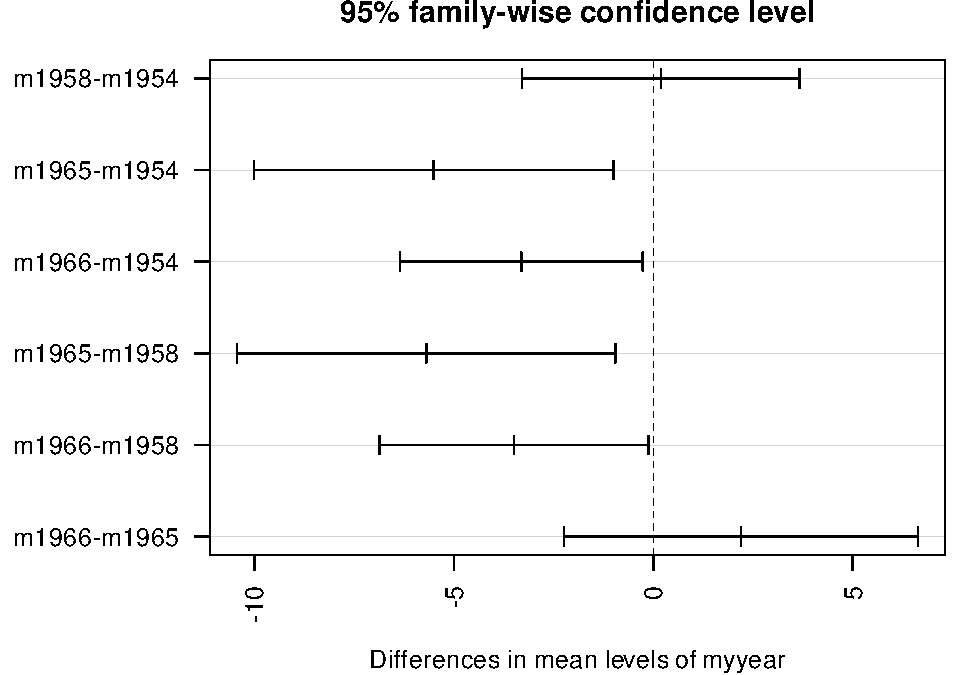
\includegraphics{Labs_BIO4158_files/figure-latex/ano-13-1.pdf}
\caption{\label{fig:ano-13}Inter-annual differences in sturgeon length}
\end{figure}

The confidence intervals, corrected for multiple tests by the Tukey method, are plotted for differences among years. Unfortunately, the labels are not all printed because they would overlap, but the order is the same as in the preceding table. The \texttt{multcomp} 📦 can produce a better plot version, but requires a bit more code:

\begin{Shaded}
\begin{Highlighting}[]
\CommentTok{\# Alternative way to compute Tukey multiple comparisons}
\CommentTok{\# set up a one{-}way ANOVA}
\NormalTok{anova\_fkl\_year \textless{}{-}}\StringTok{ }\KeywordTok{aov}\NormalTok{(fklngth }\OperatorTok{\textasciitilde{}}\StringTok{ }\NormalTok{myyear, }\DataTypeTok{data =}\NormalTok{ dam10dat)}
\CommentTok{\# set up all{-}pairs comparisons for factor \textasciigrave{}year\textquotesingle{}}

\NormalTok{meandiff \textless{}{-}}\StringTok{ }\KeywordTok{glht}\NormalTok{(anova\_fkl\_year, }\DataTypeTok{linfct =} \KeywordTok{mcp}\NormalTok{(}
  \DataTypeTok{myyear =}
    \StringTok{"Tukey"}
\NormalTok{))}
\KeywordTok{confint}\NormalTok{(meandiff)}
\end{Highlighting}
\end{Shaded}

\begin{verbatim}
## 
##   Simultaneous Confidence Intervals
## 
## Multiple Comparisons of Means: Tukey Contrasts
## 
## 
## Fit: aov(formula = fklngth ~ myyear, data = dam10dat)
## 
## Quantile = 2.5945
## 95% family-wise confidence level
##  
## 
## Linear Hypotheses:
##                    Estimate lwr      upr     
## m1958 - m1954 == 0   0.1872  -3.2724   3.6468
## m1965 - m1954 == 0  -5.5077  -9.9988  -1.0166
## m1966 - m1954 == 0  -3.3127  -6.3442  -0.2812
## m1965 - m1958 == 0  -5.6949 -10.4129  -0.9768
## m1966 - m1958 == 0  -3.4999  -6.8584  -0.1414
## m1966 - m1965 == 0   2.1950  -2.2187   6.6087
\end{verbatim}

\begin{Shaded}
\begin{Highlighting}[]
\KeywordTok{par}\NormalTok{(}\DataTypeTok{mar =} \KeywordTok{c}\NormalTok{(}\DecValTok{5}\NormalTok{, }\DecValTok{7}\NormalTok{, }\DecValTok{2}\NormalTok{, }\DecValTok{1}\NormalTok{))}
\KeywordTok{plot}\NormalTok{(meandiff)}
\end{Highlighting}
\end{Shaded}

\begin{figure}
\centering
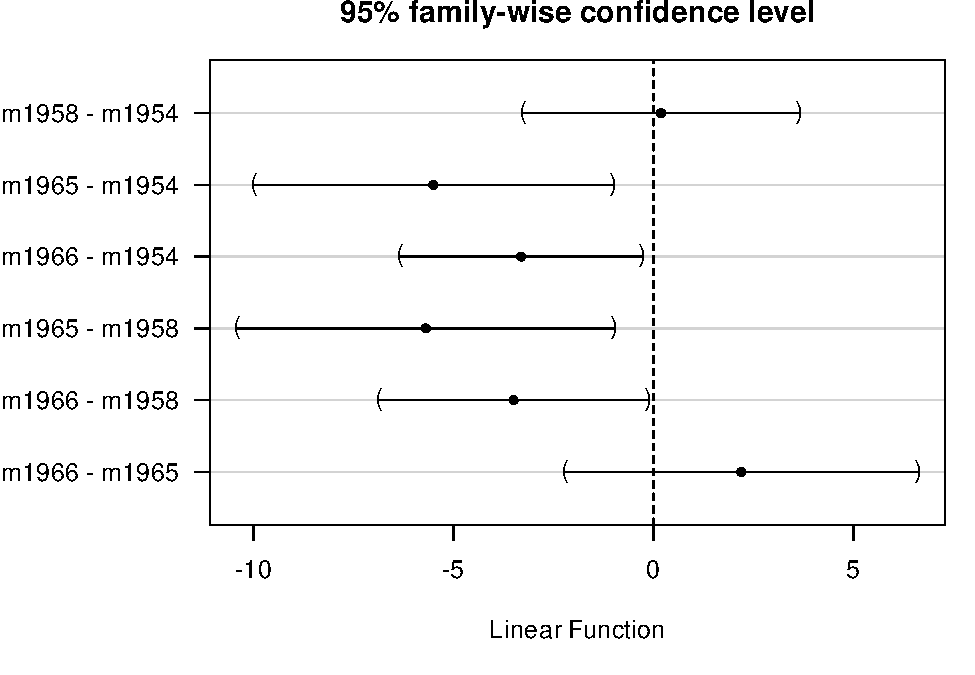
\includegraphics{Labs_BIO4158_files/figure-latex/ano-14-1.pdf}
\caption{\label{fig:ano-14}Inter-annual differences in sturgeon length}
\end{figure}

This is better. Also useful is a plot the means and their confidence intervals with the Tukey groupings shown as letters above:

\begin{Shaded}
\begin{Highlighting}[]
\CommentTok{\# Compute and plot means and Tukey CI}
\NormalTok{means \textless{}{-}}\StringTok{ }\KeywordTok{glht}\NormalTok{(}
\NormalTok{  anova\_fkl\_year,}
  \DataTypeTok{linfct =} \KeywordTok{mcp}\NormalTok{(}\DataTypeTok{myyear =} \StringTok{"Tukey"}\NormalTok{)}
\NormalTok{)}
\NormalTok{cimeans \textless{}{-}}\StringTok{ }\KeywordTok{cld}\NormalTok{(means)}
\CommentTok{\# use sufficiently large upper margin}
\CommentTok{\# plot}
\NormalTok{old\_par \textless{}{-}}\StringTok{ }\KeywordTok{par}\NormalTok{(}\DataTypeTok{mai =} \KeywordTok{c}\NormalTok{(}\DecValTok{1}\NormalTok{, }\DecValTok{1}\NormalTok{, }\FloatTok{1.25}\NormalTok{, }\DecValTok{1}\NormalTok{))}
\KeywordTok{plot}\NormalTok{(cimeans)}
\end{Highlighting}
\end{Shaded}

\begin{figure}
\centering
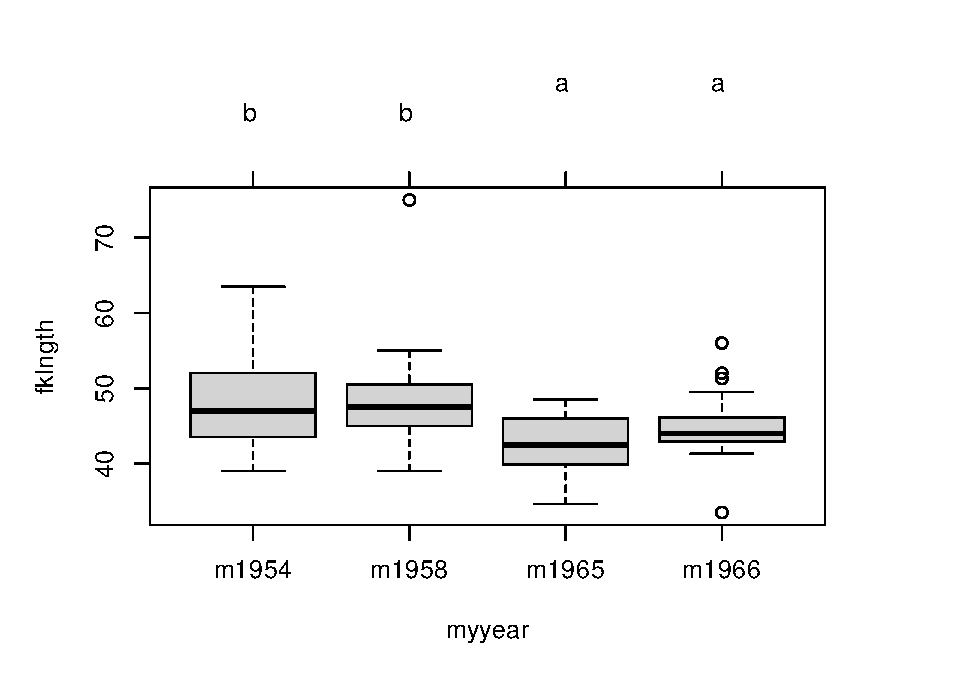
\includegraphics{Labs_BIO4158_files/figure-latex/ano-15-1.pdf}
\caption{\label{fig:ano-15}Inter-annual differences in sturgeon length}
\end{figure}

Note the letters appearing on top. Years labelled with the same letter do not differ significantly.

\hypertarget{data-transformations-and-non-parametric-anova}{%
\section{Data transformations and non-parametric ANOVA}\label{data-transformations-and-non-parametric-anova}}

In the above example to examine differences in fklngth among years , we detected evidence of non-normality and variance heterogeneity. If the assumptions underlying a parametric ANOVA are not valid, there are several options:

\begin{enumerate}
\def\labelenumi{\arabic{enumi}.}
\tightlist
\item
  if sample sizes in each group are reasonably large, parametric ANOVA is reasonably robust with respect to the normality assumption, for the same reason that the t-test is, so the results are probably not too bad;
\item
  we can transform the data;
\item
  we can go the non-parametric route.
\end{enumerate}

\begin{itemize}
\tightlist
\item
  Repeat the one-way ANOVA in the section above, but this time run the analysis on the log 10 fklngth . With this transformation, do some of the problems encountered previously disappear?
\end{itemize}

\begin{Shaded}
\begin{Highlighting}[]
\CommentTok{\# Fit anova model on log10 of fklngth and plot residual diagnostics}
\KeywordTok{par}\NormalTok{(}\DataTypeTok{mfrow =} \KeywordTok{c}\NormalTok{(}\DecValTok{2}\NormalTok{, }\DecValTok{2}\NormalTok{))}
\NormalTok{anova.model2 \textless{}{-}}\StringTok{ }\KeywordTok{lm}\NormalTok{(}\KeywordTok{log10}\NormalTok{(fklngth) }\OperatorTok{\textasciitilde{}}\StringTok{ }\NormalTok{year, }\DataTypeTok{data =}\NormalTok{ dam10dat)}
\KeywordTok{plot}\NormalTok{(anova.model2)}
\end{Highlighting}
\end{Shaded}

\begin{figure}
\centering
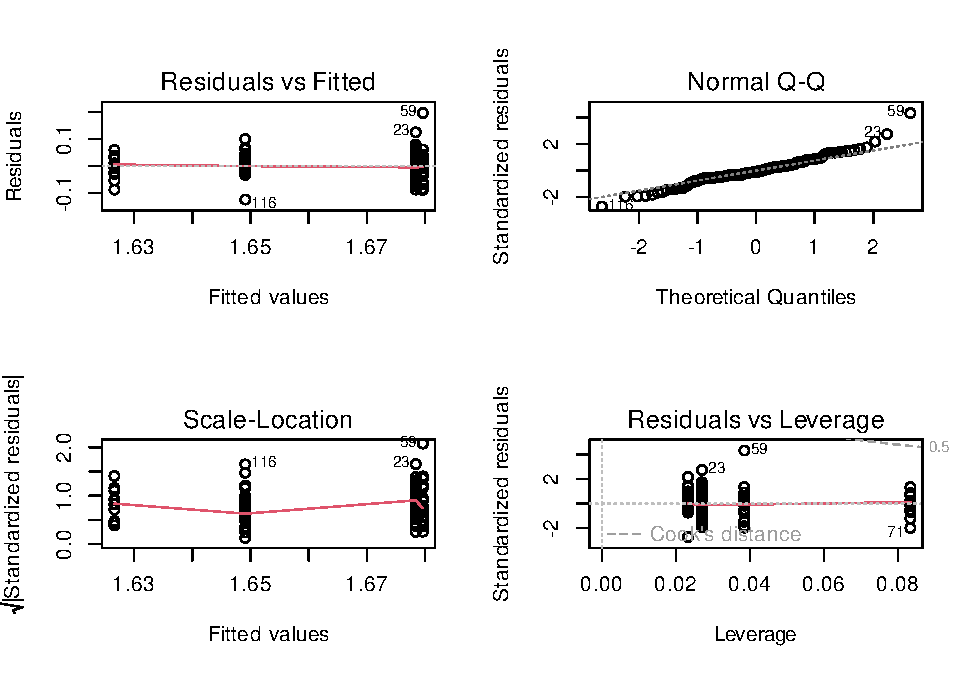
\includegraphics{Labs_BIO4158_files/figure-latex/ano-16-1.pdf}
\caption{\label{fig:ano-16}Diagnostic plots for the ANOVA of sturgeon length by year}
\end{figure}

Looking at the residuals, things look barely better than before without the log transformation. Running the Wilks-Shapiro
test for normality on the residuals, we get:

\begin{Shaded}
\begin{Highlighting}[]
\KeywordTok{shapiro.test}\NormalTok{(}\KeywordTok{residuals}\NormalTok{(anova.model2))}
\end{Highlighting}
\end{Shaded}

\begin{verbatim}
## 
##  Shapiro-Wilk normality test
## 
## data:  residuals(anova.model2)
## W = 0.96199, p-value = 0.002048
\end{verbatim}

So, it would appear that we still have some problems with the assumption of normality and are just on the border line of meeting the assumption of homogeneity of variances. You have several choices here:

\begin{enumerate}
\def\labelenumi{\arabic{enumi}.}
\tightlist
\item
  try to find a different transformation to satisfy the assumptions,
\item
  assume the data are close enough to meeting the assumptions, or
\item
  perform a non-parametric ANOVA.
\end{enumerate}

\begin{itemize}
\tightlist
\item
  The most commonly used non-parametric analog of the parametric one-way ANOVA is the Kruskall-Wallis one-way ANOVA. Perform a Kruskall-Wallis one-way ANOVA of \texttt{fklngth} , and compare these results to the parametric analysis above. What do you conclude?
\end{itemize}

\begin{Shaded}
\begin{Highlighting}[]
\KeywordTok{kruskal.test}\NormalTok{(fklngth }\OperatorTok{\textasciitilde{}}\StringTok{ }\NormalTok{year, }\DataTypeTok{data =}\NormalTok{ dam10dat)}
\end{Highlighting}
\end{Shaded}

\begin{verbatim}
## 
##  Kruskal-Wallis rank sum test
## 
## data:  fklngth by year
## Kruskal-Wallis chi-squared = 15.731, df = 3, p-value = 0.001288
\end{verbatim}

So, the conclusion is the same as with the parametric ANOVA: we reject the null that the mean rank is the same for each year. Thus, despite violation of one or more assumptions, the parametric analysis is telling us the same thing as the non-parametric analysis: the conclusion is, therefore, quite robust.

\hypertarget{dealing-with-outliers-1}{%
\section{Dealing with outliers}\label{dealing-with-outliers-1}}

Our preliminary analysis of the relationship between \texttt{fklngth} and \texttt{year} suggested there might be some outliers in the data. These were evident in the box plots of \texttt{fklngth} by \texttt{year} and flagged as cases 59, 23 and 87 in the residual probability plot and residual-fit plot. In general, you have to have very good reasons for removing outliers from a data set (e.g., you know there was a mistake made in the data collection/entry). However, it is often useful to know how the analysis changes if you remove the outliers from the data set.

\begin{itemize}
\tightlist
\item
  Repeat the original ANOVA of \texttt{fklngth} by \texttt{year} but work with a subset of the data without the outliers. Have any of the conclusions changed?
\end{itemize}

\begin{Shaded}
\begin{Highlighting}[]
\NormalTok{damsubset \textless{}{-}}\StringTok{ }\NormalTok{dam10dat[}\OperatorTok{{-}}\KeywordTok{c}\NormalTok{(}\DecValTok{23}\NormalTok{, }\DecValTok{59}\NormalTok{, }\DecValTok{87}\NormalTok{), ] }\CommentTok{\# removes obs 23, 59 and 87}
\NormalTok{aov\_damsubset \textless{}{-}}\StringTok{ }\KeywordTok{aov}\NormalTok{(fklngth }\OperatorTok{\textasciitilde{}}\StringTok{ }\KeywordTok{as.factor}\NormalTok{(year), damsubset)}
\KeywordTok{summary}\NormalTok{(aov\_damsubset)}
\end{Highlighting}
\end{Shaded}

\begin{verbatim}
##                  Df Sum Sq Mean Sq F value   Pr(>F)    
## as.factor(year)   3  367.5  122.50   6.894 0.000267 ***
## Residuals       111 1972.4   17.77                     
## ---
## Signif. codes:  0 '***' 0.001 '**' 0.01 '*' 0.05 '.' 0.1 ' ' 1
\end{verbatim}

\begin{Shaded}
\begin{Highlighting}[]
\KeywordTok{shapiro.test}\NormalTok{(}\KeywordTok{residuals}\NormalTok{(aov\_damsubset))}
\end{Highlighting}
\end{Shaded}

\begin{verbatim}
## 
##  Shapiro-Wilk normality test
## 
## data:  residuals(aov_damsubset)
## W = 0.98533, p-value = 0.2448
\end{verbatim}

\begin{Shaded}
\begin{Highlighting}[]
\KeywordTok{leveneTest}\NormalTok{(fklngth }\OperatorTok{\textasciitilde{}}\StringTok{ }\NormalTok{year, damsubset)}
\end{Highlighting}
\end{Shaded}

\begin{verbatim}
## Levene's Test for Homogeneity of Variance (center = median)
##        Df F value   Pr(>F)   
## group   3  4.6237 0.004367 **
##       111                    
## ---
## Signif. codes:  0 '***' 0.001 '**' 0.01 '*' 0.05 '.' 0.1 ' ' 1
\end{verbatim}

Elimination of three outliers, in this case, makes things better in terms of the normality assumption, but does not improve the
variances. Moreover, the fact that the conclusion drawn from the original ANOVA with outliers retained does not change upon their removal reinforces the fact that there is no good reason to remove the points. Instead of a Kruskall-Wallis rank-based test, a permutation test could be used.

\hypertarget{permutation-test}{%
\section{Permutation test}\label{permutation-test}}

This is an example for a more complex way of doing permutation that we used when \texttt{lmPerm} was not available.

\begin{Shaded}
\begin{Highlighting}[]
\CommentTok{\#\#\#\#\#\#\#\#\#\#\#\#\#\#\#\#\#\#\#\#\#\#\#\#\#\#\#\#\#\#\#\#\#\#\#\#\#\#\#\#\#\#\#\#\#\#\#\#\#\#\#\#\#\#\#\#\#\#\#\#\#}
\CommentTok{\# Permutation Test for one{-}way ANOVA}
\CommentTok{\# modified from code written by David C. Howell}
\CommentTok{\# http://www.uvm.edu/\textasciitilde{}dhowell/StatPages/}
\CommentTok{\# More\_Stuff/Permutation\%20Anova/PermTestsAnova.html}
\CommentTok{\# set desired number of permutations}
\NormalTok{nreps \textless{}{-}}\StringTok{ }\DecValTok{500}
\CommentTok{\# to simplify reuse of this code, copy desired dataframe to mydata}
\NormalTok{mydata \textless{}{-}}\StringTok{ }\NormalTok{dam10dat}
\CommentTok{\# copy model formula to myformula}
\NormalTok{myformula \textless{}{-}}\StringTok{ }\KeywordTok{as.formula}\NormalTok{(}\StringTok{"fklngth \textasciitilde{} year"}\NormalTok{)}
\CommentTok{\# copy dependent variable vector to mydep}
\NormalTok{mydep \textless{}{-}}\StringTok{ }\NormalTok{mydata}\OperatorTok{$}\NormalTok{fklngth}
\CommentTok{\# copy independent variable vector to myindep}
\NormalTok{myindep \textless{}{-}}\StringTok{ }\KeywordTok{as.factor}\NormalTok{(mydata}\OperatorTok{$}\NormalTok{year)}
\CommentTok{\#\#\#\#\#\#\#\#\#\#\#\#\#\#\#\#\#\#\#\#\#\#\#\#\#\#\#\#\#\#\#\#\#\#\#\#\#\#\#\#\#\#\#\#\#\#\#\#}
\CommentTok{\# You should not need to modify code chunk below}
\CommentTok{\#\#\#\#\#\#\#\#\#\#\#\#\#\#\#\#\#\#\#\#\#\#\#\#\#\#\#\#\#\#\#\#\#\#\#\#\#\#\#\#\#\#\#\#\#\#\#\#}
\CommentTok{\# Compute observed F value for original sample}
\NormalTok{mod1 \textless{}{-}}\StringTok{ }\KeywordTok{lm}\NormalTok{(myformula, }\DataTypeTok{data =}\NormalTok{ mydata) }\CommentTok{\# Standard Anova}
\NormalTok{sum\_anova \textless{}{-}}\StringTok{ }\KeywordTok{summary}\NormalTok{(}\KeywordTok{aov}\NormalTok{(mod1)) }\CommentTok{\# Save summary to variable}
\NormalTok{obs\_f \textless{}{-}}\StringTok{ }\NormalTok{sum\_anova[[}\DecValTok{1}\NormalTok{]]}\OperatorTok{$}\StringTok{"F value"}\NormalTok{[}\DecValTok{1}\NormalTok{] }\CommentTok{\# Save observed F value}
\CommentTok{\# Print standard ANOVA results}
\KeywordTok{cat}\NormalTok{(}
  \StringTok{" The standard ANOVA for these data follows "}\NormalTok{,}
  \StringTok{"}\CharTok{\textbackslash{}n}\StringTok{"}
\NormalTok{)}

\KeywordTok{print}\NormalTok{(sum\_anova, }\StringTok{"}\CharTok{\textbackslash{}n}\StringTok{"}\NormalTok{)}
\KeywordTok{cat}\NormalTok{(}\StringTok{"}\CharTok{\textbackslash{}n}\StringTok{"}\NormalTok{)}
\KeywordTok{cat}\NormalTok{(}\StringTok{"}\CharTok{\textbackslash{}n}\StringTok{"}\NormalTok{)}
\KeywordTok{print}\NormalTok{(}\StringTok{"Resampling as in Manly with unrestricted sampling of observations. "}\NormalTok{)}

\CommentTok{\# Now start resampling}
\NormalTok{boot\_f \textless{}{-}}\StringTok{ }\KeywordTok{numeric}\NormalTok{(nreps) }\CommentTok{\# initalize vector to receive permuted}
\NormalTok{values}
\NormalTok{boot\_f[}\DecValTok{1}\NormalTok{] \textless{}{-}}\StringTok{ }\NormalTok{obs\_f}
\ControlFlowTok{for}\NormalTok{ (i }\ControlFlowTok{in} \DecValTok{2}\OperatorTok{:}\NormalTok{nreps) \{}
\NormalTok{  newdependent \textless{}{-}}\StringTok{ }\KeywordTok{sample}\NormalTok{(mydep, }\KeywordTok{length}\NormalTok{(mydep)) }\CommentTok{\# randomize dep}
\NormalTok{  var}
\NormalTok{  mod2 \textless{}{-}}\StringTok{ }\KeywordTok{lm}\NormalTok{(newdependent }\OperatorTok{\textasciitilde{}}\StringTok{ }\NormalTok{myindep) }\CommentTok{\# refit model}
\NormalTok{  b \textless{}{-}}\StringTok{ }\KeywordTok{summary}\NormalTok{(}\KeywordTok{aov}\NormalTok{(mod2))}
\NormalTok{  boot\_f[i] \textless{}{-}}\StringTok{ }\NormalTok{b[[}\DecValTok{1}\NormalTok{]]}\OperatorTok{$}\StringTok{"F value"}\NormalTok{[}\DecValTok{1}\NormalTok{] }\CommentTok{\# store F stats}
\NormalTok{\}}
\NormalTok{permprob \textless{}{-}}\StringTok{ }\KeywordTok{length}\NormalTok{(boot\_f[boot\_f }\OperatorTok{\textgreater{}=}\StringTok{ }\NormalTok{obs\_f]) }\OperatorTok{/}\StringTok{ }\NormalTok{nreps}
\KeywordTok{cat}\NormalTok{(}
  \StringTok{" The permutation probability value is: "}\NormalTok{, permprob,}
  \StringTok{"}\CharTok{\textbackslash{}n}\StringTok{"}
\NormalTok{)}
\CommentTok{\# end of code chunk for permutation}
\end{Highlighting}
\end{Shaded}

Version \texttt{lmPerm} du test de permutation.

\begin{Shaded}
\begin{Highlighting}[]
\CommentTok{\#\# lmPerm version of permutation test}
\KeywordTok{library}\NormalTok{(lmPerm)}
\CommentTok{\# for generality, copy desired dataframe to mydata}
\CommentTok{\# and model formula to myformula}
\NormalTok{mydata \textless{}{-}}\StringTok{ }\NormalTok{dam10dat}
\NormalTok{myformula \textless{}{-}}\StringTok{ }\KeywordTok{as.formula}\NormalTok{(}\StringTok{"fklngth \textasciitilde{} year"}\NormalTok{)}
\CommentTok{\# Fit desired model on the desired dataframe}
\NormalTok{mymodel \textless{}{-}}\StringTok{ }\KeywordTok{lm}\NormalTok{(myformula, }\DataTypeTok{data =}\NormalTok{ mydata)}
\CommentTok{\# Calculate permutation p{-}value}
\KeywordTok{anova}\NormalTok{(}\KeywordTok{lmp}\NormalTok{(myformula, }\DataTypeTok{data =}\NormalTok{ mydata, }\DataTypeTok{perm =} \StringTok{"Prob"}\NormalTok{, }\DataTypeTok{center =} \OtherTok{FALSE}\NormalTok{, }\DataTypeTok{Ca =} \FloatTok{0.001}\NormalTok{))}
\end{Highlighting}
\end{Shaded}

\hypertarget{multiway-anova-factorial-and-nested-designs}{%
\chapter{Multiway ANOVA: factorial and nested designs}\label{multiway-anova-factorial-and-nested-designs}}

After completing this laboratory exercise, you should be able to:

\begin{itemize}
\tightlist
\item
  Use R to do parametric ANOVAs for 2-way factorial designs with replication.
\item
  Use R to do 2-way factorial design ANOVA without replication
\item
  Use R to do parametric ANOVAs for nested designs with replication.
\item
  Use R to do non-parametric 2-way ANOVAs
\item
  Use R to do multiway pairwise comparisons
\end{itemize}

Be aware that there are a large number of possible ANOVA designs,
many of which can be handled by R: this laboratory is

\hypertarget{set-anomul}{%
\section{R packages and data needed}\label{set-anomul}}

For this lab you need:

\begin{itemize}
\tightlist
\item
  R packages:

  \begin{itemize}
  \tightlist
  \item
    tidyverse
  \item
    multicomp
  \item
    car
  \item
    effects
  \end{itemize}
\item
  data files:

  \begin{itemize}
  \tightlist
  \item
    Stu2wdat.csv
  \item
    Stu2mdat.csv
  \item
    nr2wdat.csv
  \item
    nestdat.csv
  \item
    wmcdat2.csv
  \item
    wmc2dat2.csv
  \end{itemize}
\end{itemize}

\begin{Shaded}
\begin{Highlighting}[]
\KeywordTok{library}\NormalTok{(multcomp)}
\KeywordTok{library}\NormalTok{(car)}
\KeywordTok{library}\NormalTok{(tidyverse)}
\end{Highlighting}
\end{Shaded}

\begin{verbatim}
## -- Attaching packages ------------------------------------------------------------------------------------------------------------------ tidyverse 1.3.1 --
\end{verbatim}

\begin{verbatim}
## v tibble  3.1.6     v dplyr   1.0.7
## v tidyr   1.1.4     v stringr 1.4.0
## v readr   2.1.0     v forcats 0.5.1
## v purrr   0.3.4
\end{verbatim}

\begin{verbatim}
## -- Conflicts --------------------------------------------------------------------------------------------------------------------- tidyverse_conflicts() --
## x dplyr::filter() masks stats::filter()
## x dplyr::lag()    masks stats::lag()
## x dplyr::recode() masks car::recode()
## x dplyr::select() masks MASS::select()
## x purrr::some()   masks car::some()
\end{verbatim}

\begin{Shaded}
\begin{Highlighting}[]
\KeywordTok{library}\NormalTok{(effects)}
\end{Highlighting}
\end{Shaded}

\begin{verbatim}
## lattice theme set by effectsTheme()
## See ?effectsTheme for details.
\end{verbatim}

\hypertarget{two-way-factorial-design-with-replication}{%
\section{Two-way factorial design with replication}\label{two-way-factorial-design-with-replication}}

Many experiments are designed to investigate the joint effects of several different factors: in a two-way ANOVA, we examine the effect of two factors, but in principle the analysis can be extended to three, four or even five factors, although interpreting the results from 4- and 5-way ANOVAs can be very difficult.

Suppose that we are interested in the effects of two factors: \texttt{location} (Cumberland House and The Pas) and \texttt{sex} (male or female) on sturgeon size (data can be found in \texttt{Stu2wdat.csv}). Note that because the sample sizes are not the same for each group, this is an unbalanced design. Note also that there are missing data for some of the variables, meaning that not every measurement was made on every fish.

\hypertarget{fixed-effects-anova-model-i}{%
\subsection{Fixed effects ANOVA (Model I)}\label{fixed-effects-anova-model-i}}

\begin{itemize}
\tightlist
\item
  Begin by having a look at the data by generating box plots of \texttt{rdwght} for \texttt{sex} and \texttt{location} from the file \texttt{Stu2wdat.csv} .
\end{itemize}

\begin{verbatim}
## Warning: Removed 4 rows containing non-finite values (stat_boxplot).
\end{verbatim}

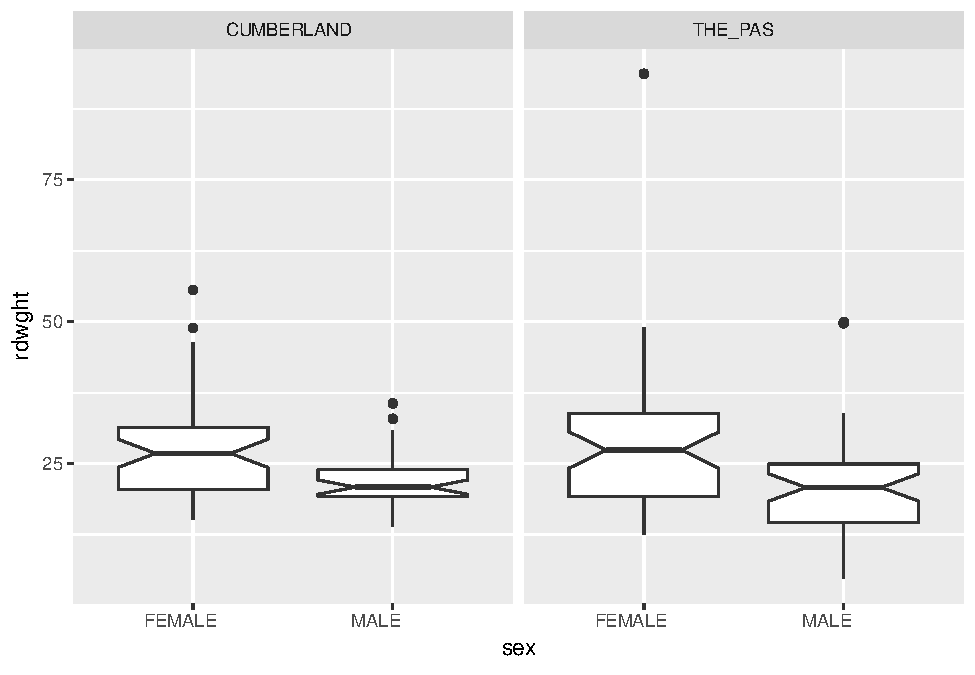
\includegraphics{Labs_BIO4158_files/figure-latex/unnamed-chunk-41-1.pdf}

From this, it appears as though females might be larger at both locations. It's difficult to get an idea of whether fish differ in size between the two locations. The presence of outliers on these plots suggests there might be problems meeting normality assumptions for the residuals.

\begin{itemize}
\tightlist
\item
  Generate summary statistics for rdwght by sex and location .
\end{itemize}

\begin{Shaded}
\begin{Highlighting}[]
\NormalTok{Stu2wdat \textless{}{-}}\StringTok{ }\KeywordTok{read.csv}\NormalTok{(}\StringTok{"data/Stu2wdat.csv"}\NormalTok{)}
\KeywordTok{aggregate}\NormalTok{(rdwght }\OperatorTok{\textasciitilde{}}\StringTok{ }\NormalTok{sex }\OperatorTok{+}\StringTok{ }\NormalTok{location, }\DataTypeTok{data =}\NormalTok{ Stu2wdat, }\DataTypeTok{FUN =} \StringTok{"summary"}\NormalTok{)}
\end{Highlighting}
\end{Shaded}

\begin{verbatim}
##            sex     location rdwght.Min. rdwght.1st Qu. rdwght.Median
## 1 FEMALE       CUMBERLAND      15.10000       20.40000      26.80000
## 2 MALE         CUMBERLAND      14.00000       19.22500      20.85000
## 3 FEMALE       THE_PAS         12.54000       19.14000      27.39000
## 4 MALE         THE_PAS          4.73000       14.63000      20.79000
##   rdwght.Mean rdwght.3rd Qu. rdwght.Max.
## 1    27.37347       31.40000    55.60000
## 2    22.14118       23.90000    35.60000
## 3    27.97717       33.88000    93.72000
## 4    20.64652       24.94250    49.94000
\end{verbatim}

The summary statistics confirm our interpretation of the box plots: females appear to be larger than males, and differences in fish size between locations are small.

\begin{itemize}
\tightlist
\item
  Using the file \texttt{Stu2wdat.csv} , do a two-way factorial ANOVA:
\end{itemize}

\begin{Shaded}
\begin{Highlighting}[]
\CommentTok{\# Fit anova model and plot residual diagnostics}
\CommentTok{\# but first, save current par and set graphic page to hold 4 graphs}
\NormalTok{opar \textless{}{-}}\StringTok{ }\KeywordTok{par}\NormalTok{(}\DataTypeTok{mfrow =} \KeywordTok{c}\NormalTok{(}\DecValTok{2}\NormalTok{, }\DecValTok{2}\NormalTok{))}
\NormalTok{anova.model1 \textless{}{-}}\StringTok{ }\KeywordTok{lm}\NormalTok{(rdwght }\OperatorTok{\textasciitilde{}}\StringTok{ }\NormalTok{sex }\OperatorTok{+}\StringTok{ }\NormalTok{location }\OperatorTok{+}\StringTok{ }\NormalTok{sex}\OperatorTok{:}\NormalTok{location,}
  \DataTypeTok{contrasts =} \KeywordTok{list}\NormalTok{(}\DataTypeTok{sex =}\NormalTok{ contr.sum, }\DataTypeTok{location =}\NormalTok{ contr.sum),}
  \DataTypeTok{data =}\NormalTok{ Stu2wdat}
\NormalTok{)}
\KeywordTok{anova}\NormalTok{(anova.model1)}
\end{Highlighting}
\end{Shaded}

\begin{verbatim}
## Analysis of Variance Table
## 
## Response: rdwght
##               Df  Sum Sq Mean Sq F value    Pr(>F)    
## sex            1  1839.6 1839.55 18.6785 2.569e-05 ***
## location       1     4.3    4.26  0.0433    0.8355    
## sex:location   1    48.7   48.69  0.4944    0.4829    
## Residuals    178 17530.4   98.49                      
## ---
## Signif. codes:  0 '***' 0.001 '**' 0.01 '*' 0.05 '.' 0.1 ' ' 1
\end{verbatim}

\begin{rmdwarning}
Be careful here. R gives you the sequential sums of squares (Type I) and associated Mean squares and probabilities. These are not to be trusted unless the design is perfectly balanced. In this case, there are varying numbers of observations across sex and location combinations and therefore the design is not balanced.
\end{rmdwarning}

What you want are the partial sums of squares (type III). The easiest way to get them is to use the Anova() function in the \texttt{car} 📦 package (note the subtle difference, \texttt{Anova()} is not the same as \texttt{anova()}, remember case matters in R.). However, this is not enough by itself. To get the proper values for the type III sums of square, one also needs to specify contrasts, hence the cryptic \texttt{contrasts\ =\ list(sex\ =\ contr.sum,location\ =\ contr.sum)}.

\begin{Shaded}
\begin{Highlighting}[]
\KeywordTok{library}\NormalTok{(car)}
\KeywordTok{Anova}\NormalTok{(anova.model1, }\DataTypeTok{type =} \DecValTok{3}\NormalTok{)}
\end{Highlighting}
\end{Shaded}

\begin{verbatim}
## Anova Table (Type III tests)
## 
## Response: rdwght
##              Sum Sq  Df   F value    Pr(>F)    
## (Intercept)  106507   1 1081.4552 < 2.2e-16 ***
## sex            1745   1   17.7220 4.051e-05 ***
## location          9   1    0.0891    0.7656    
## sex:location     49   1    0.4944    0.4829    
## Residuals     17530 178                        
## ---
## Signif. codes:  0 '***' 0.001 '**' 0.01 '*' 0.05 '.' 0.1 ' ' 1
\end{verbatim}

On the basis of the ANOVA, there is no reason to reject two null hypotheses: (1) that the effect of sex (if any) does not depend on location (no interaction), and (2) that there is no difference in the size of sturgeon (pooled over sex ) between the two locations . On the other hand, we reject the null hypothesis that there is no difference in size between male and female sturgeon (pooled over location ), precisely as expected from the graphs.

\begin{Shaded}
\begin{Highlighting}[]
\KeywordTok{par}\NormalTok{(}\DataTypeTok{mfrow =} \KeywordTok{c}\NormalTok{(}\DecValTok{2}\NormalTok{, }\DecValTok{2}\NormalTok{))}
\KeywordTok{plot}\NormalTok{(anova.model1)}
\end{Highlighting}
\end{Shaded}

\begin{figure}
\centering
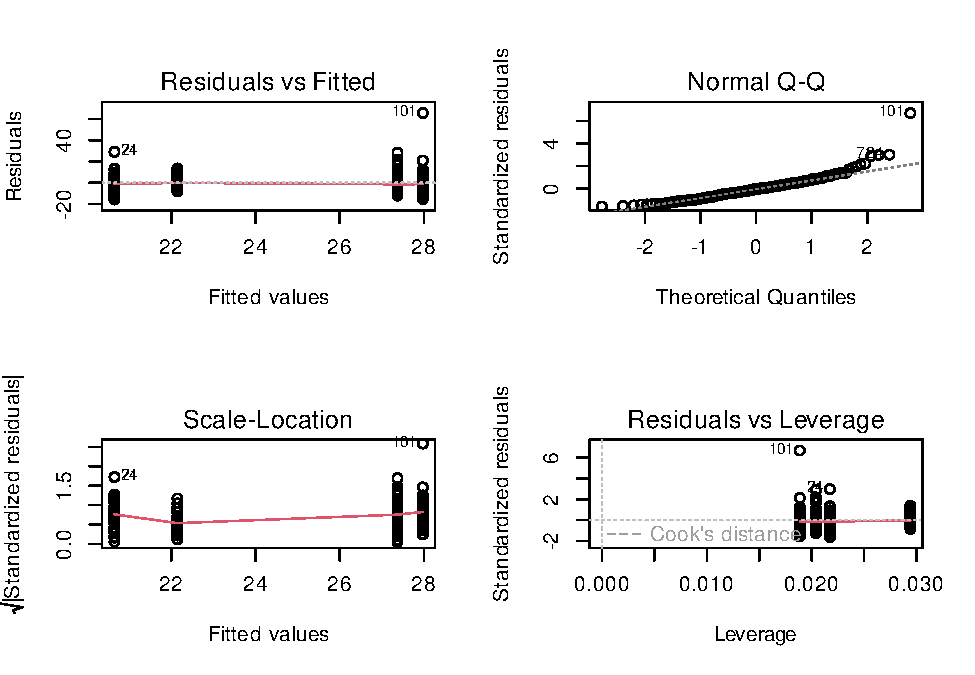
\includegraphics{Labs_BIO4158_files/figure-latex/unnamed-chunk-46-1.pdf}
\caption{\label{fig:unnamed-chunk-46}Checking model assumptions for ANOVA model1}
\end{figure}

As usual, we cannot accept the above results without first ensuring that the assumptions of ANOVA are met. Examination of the residuals plots above shows that the residuals are reasonably normally distributed, with the exception of three potential outliers flagged on the QQ plot (cases 101, 24, \& 71; the latter two are on top of one another). However, Cook's distances are not large for these (the 0.5 contour is not even visible on the plot), so there is little indication that these are a concern.The residuals vs fit plot shows that the spread of residuals is about equal over the range of the fitted values, again with the exception of a few cases. When we test for normality of residuals we get:

\begin{Shaded}
\begin{Highlighting}[]
\KeywordTok{shapiro.test}\NormalTok{(}\KeywordTok{residuals}\NormalTok{(anova.model1))}
\end{Highlighting}
\end{Shaded}

\begin{verbatim}
## 
##  Shapiro-Wilk normality test
## 
## data:  residuals(anova.model1)
## W = 0.87213, p-value = 2.619e-11
\end{verbatim}

So, there is evidence of non-normality in the residuals.

We will use the Levene's test to examine the assumption of homogeneity of variances, just as we did with the 1-way anova.

\begin{Shaded}
\begin{Highlighting}[]
\KeywordTok{leveneTest}\NormalTok{(rdwght }\OperatorTok{\textasciitilde{}}\StringTok{ }\NormalTok{sex }\OperatorTok{*}\StringTok{ }\NormalTok{location, }\DataTypeTok{data =}\NormalTok{ Stu2wdat)}
\end{Highlighting}
\end{Shaded}

\begin{verbatim}
## Levene's Test for Homogeneity of Variance (center = median)
##        Df F value  Pr(>F)  
## group   3  3.8526 0.01055 *
##       178                  
## ---
## Signif. codes:  0 '***' 0.001 '**' 0.01 '*' 0.05 '.' 0.1 ' ' 1
\end{verbatim}

If the assumption of homogeneity of variances was valid, we would be accepting the null that the mean of the absolute values of residuals does not vary among levels of sex and location (i.e., group ). The above table shows that the hypothesis is rejected and we conclude there is evidence of heteroscedascticity. All in all, there is some evidence that several important assumptions have been violated. However, whether these violations are sufficiently large to invalidate our conclusions remains to be seen.

\begin{rmdcode}
Repeat this procedure using the data file Stu2mdat.Rdata . Now what do you conclude? Suppose you wanted to compare the sizes of males and females: in what way would these comparisons differ between Stu2wdat.Rdata and Stu2mdat.Rdata ?
\end{rmdcode}

\begin{verbatim}
## 
## Call:
## lm(formula = rdwght ~ sex + location + sex:location, data = Stu2mdat, 
##     contrasts = list(sex = contr.sum, location = contr.sum))
## 
## Residuals:
##     Min      1Q  Median      3Q     Max 
## -15.917  -6.017  -0.580   4.445  65.743 
## 
## Coefficients:
##                Estimate Std. Error t value Pr(>|t|)    
## (Intercept)     24.5346     0.7461  32.885  < 2e-16 ***
## sex1            -0.5246     0.7461  -0.703    0.483    
## location1        0.2227     0.7461   0.299    0.766    
## sex1:location1   3.1407     0.7461   4.210 4.05e-05 ***
## ---
## Signif. codes:  0 '***' 0.001 '**' 0.01 '*' 0.05 '.' 0.1 ' ' 1
## 
## Residual standard error: 9.924 on 178 degrees of freedom
##   (4 observations deleted due to missingness)
## Multiple R-squared:  0.09744,    Adjusted R-squared:  0.08223 
## F-statistic: 6.405 on 3 and 178 DF,  p-value: 0.0003817
\end{verbatim}

Note that in this case, we see that at Cumberland House, females are larger than males, whereas the opposite is true in The Pas (you can confirm this observation by generating summary statistics). What happens with the ANOVA (remember, you want Type III sum of squares)?

\begin{verbatim}
## Anova Table (Type III tests)
## 
## Response: rdwght
##              Sum Sq  Df   F value    Pr(>F)    
## (Intercept)  106507   1 1081.4552 < 2.2e-16 ***
## sex              49   1    0.4944    0.4829    
## location          9   1    0.0891    0.7656    
## sex:location   1745   1   17.7220 4.051e-05 ***
## Residuals     17530 178                        
## ---
## Signif. codes:  0 '***' 0.001 '**' 0.01 '*' 0.05 '.' 0.1 ' ' 1
\end{verbatim}

In this case, the interaction term \texttt{sex:location} is significant but the main effects are not significant.

\begin{itemize}
\tightlist
\item
  You might find it useful here to generate plots for the two data files to compare the interactions between \texttt{sex} and \texttt{location}. The effect plot shows the relationship between means for each combination of factors (also called cell means). Generate an effect plot for the two models using the \texttt{allEffects()} command from the \texttt{effects} 📦 package:
\end{itemize}

\begin{Shaded}
\begin{Highlighting}[]
\KeywordTok{library}\NormalTok{(effects)}
\KeywordTok{allEffects}\NormalTok{(anova.model1)}
\end{Highlighting}
\end{Shaded}

\begin{verbatim}
##  model: rdwght ~ sex + location + sex:location
## 
##  sex*location effect
##               location
## sex            CUMBERLAND   THE_PAS     
##   FEMALE           27.37347     27.97717
##   MALE             22.14118     20.64652
\end{verbatim}

\begin{Shaded}
\begin{Highlighting}[]
\KeywordTok{plot}\NormalTok{(}\KeywordTok{allEffects}\NormalTok{(anova.model1), }\StringTok{"sex:location"}\NormalTok{)}
\end{Highlighting}
\end{Shaded}

\begin{figure}
\centering
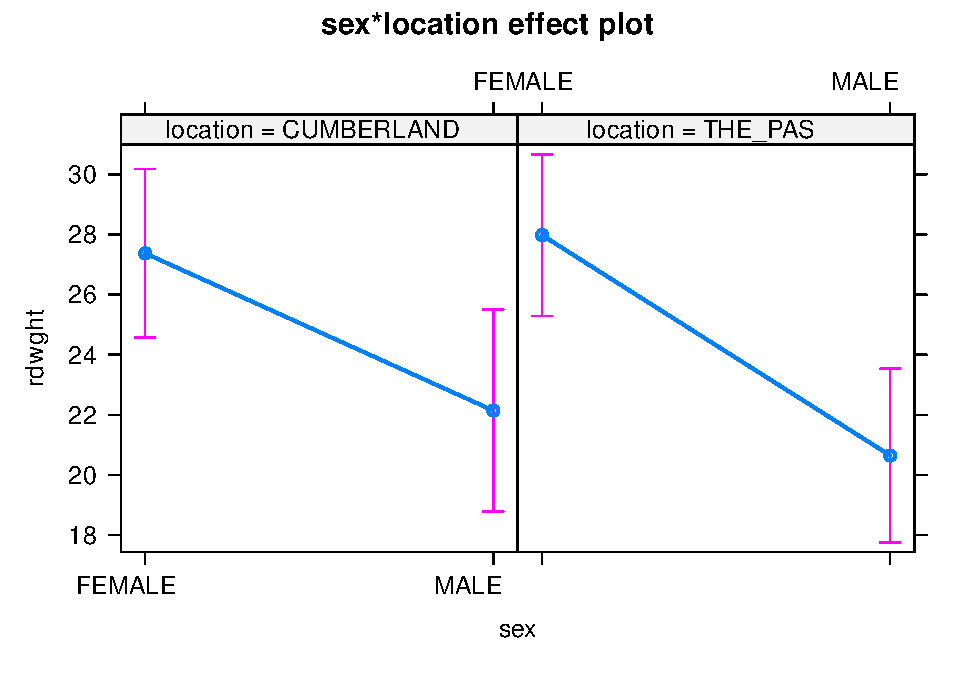
\includegraphics{Labs_BIO4158_files/figure-latex/unnamed-chunk-53-1.pdf}
\caption{\label{fig:unnamed-chunk-53}Effet du sexe et du lieu sur le poids des esturgeons}
\end{figure}

\begin{Shaded}
\begin{Highlighting}[]
\KeywordTok{allEffects}\NormalTok{(anova.model2)}
\end{Highlighting}
\end{Shaded}

\begin{verbatim}
##  model: rdwght ~ sex + location + sex:location
## 
##  sex*location effect
##               location
## sex            CUMBERLAND   THE_PAS     
##   FEMALE           27.37347     20.64652
##   MALE             22.14118     27.97717
\end{verbatim}

\begin{Shaded}
\begin{Highlighting}[]
\KeywordTok{plot}\NormalTok{(}\KeywordTok{allEffects}\NormalTok{(anova.model2), }\StringTok{"sex:location"}\NormalTok{)}
\end{Highlighting}
\end{Shaded}

\begin{figure}
\centering
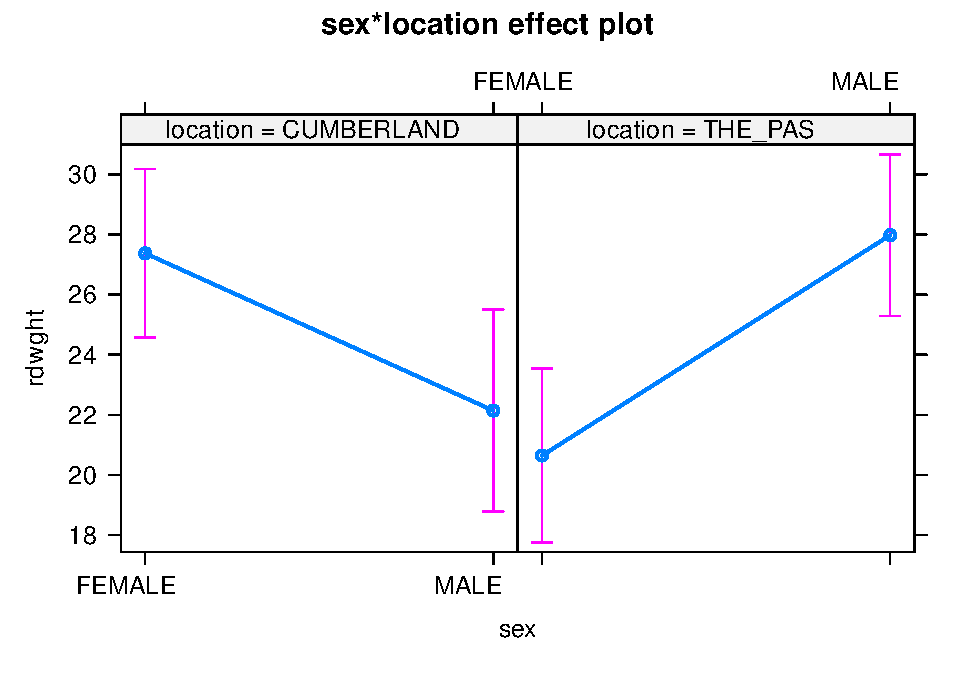
\includegraphics{Labs_BIO4158_files/figure-latex/unnamed-chunk-54-1.pdf}
\caption{\label{fig:unnamed-chunk-54}Effet du sexe et du lieu sur le poids des esturgeons}
\end{figure}

There is a very large difference between the results from \texttt{Stu2wdat} and \texttt{Stu2mdat}. In the former case, because there is no significant interaction, we can essentially pool over the levels of factor 1 (\texttt{sex}, say) to test for the effects of location , or over the levels of factor 2 (\texttt{location}) to test for the effects of sex . In fact, if we do so and simply run a one-way ANOVA on the \texttt{Stu2wdat} data with sex as the grouping variable, we get:

\begin{Shaded}
\begin{Highlighting}[]
\KeywordTok{Anova}\NormalTok{(}\KeywordTok{aov}\NormalTok{(rdwght }\OperatorTok{\textasciitilde{}}\StringTok{ }\NormalTok{sex, }\DataTypeTok{data =}\NormalTok{ Stu2wdat), }\DataTypeTok{type =} \DecValTok{3}\NormalTok{)}
\end{Highlighting}
\end{Shaded}

\begin{verbatim}
## Anova Table (Type III tests)
## 
## Response: rdwght
##             Sum Sq  Df F value    Pr(>F)    
## (Intercept)  78191   1 800.440 < 2.2e-16 ***
## sex           1840   1  18.831 2.377e-05 ***
## Residuals    17583 180                      
## ---
## Signif. codes:  0 '***' 0.001 '**' 0.01 '*' 0.05 '.' 0.1 ' ' 1
\end{verbatim}

Note that here the residual sum of squares (17583) is only slightly higher than for the 2-way model (17530), simply because, in the 2-way model, only a small fraction of the explained sums of squares is due to the location main effect or the sex:LOCATION interaction. On the other hand, if you try the same trick with \texttt{stu2mdat}, you get:

\begin{Shaded}
\begin{Highlighting}[]
\KeywordTok{Anova}\NormalTok{(}\KeywordTok{aov}\NormalTok{(rdwght }\OperatorTok{\textasciitilde{}}\StringTok{ }\NormalTok{sex, }\DataTypeTok{data =}\NormalTok{ Stu2mdat), }\DataTypeTok{type =} \DecValTok{3}\NormalTok{)}
\end{Highlighting}
\end{Shaded}

\begin{verbatim}
## Anova Table (Type III tests)
## 
## Response: rdwght
##             Sum Sq  Df  F value Pr(>F)    
## (Intercept)  55251   1 515.0435 <2e-16 ***
## sex            113   1   1.0571 0.3053    
## Residuals    19309 180                    
## ---
## Signif. codes:  0 '***' 0.001 '**' 0.01 '*' 0.05 '.' 0.1 ' ' 1
\end{verbatim}

Here, the residuals sum of squares (19309) is much larger than in the 2-way model (17530), because most of the explained sums of squares is due to the interaction. Note that if we did this, we would conclude that male and female sturgeons don't differ in size. But in fact they do: it's just that the difference is in different directions, depending on location. This is why it is always dangerous to try and make too much of main effects in the presence of interactions!

\hypertarget{mixed-effects-anova-model-iii}{%
\subsection{Mixed effects ANOVA (Model III)}\label{mixed-effects-anova-model-iii}}

We have neglected an important component in the above analyses, and that is related to the type of ANOVA model we wish to run. In this example, Location could be considered a random effect, whereas sex is a fixed effect (because it is ``fixed'' biologically), and so this model could be treated as a mixed model (Model III) ANOVA. Note that in these analyses, R treats analyses by default as Model I ANOVA, so that the main effects and the interaction are tested over the residuals mean square. Recall, however, that in a Model III ANOVA, main effects are tested over the interaction mean square or the pooled interaction mean square and residual mean square (depending on which statistician you consult!)

\begin{itemize}
\tightlist
\item
  Working with the \texttt{Stu2wdat} data, rebuild the ANOVA table for \texttt{rdwght}
  for the situation in which \texttt{location} is a random factor and \texttt{sex} is a
  fixed factor. To do this, you need to recalculate the F-ratio for sex using the \texttt{sex:location} interaction mean square instead of the residual mean square. This is most easily accomplished by hand, making sure you are working with the Type III Sums of squares ANOVA table.
\end{itemize}

\begin{verbatim}
## Anova Table (Type III tests)
## 
## Response: rdwght
##              Sum Sq  Df   F value    Pr(>F)    
## (Intercept)  106507   1 1081.4552 < 2.2e-16 ***
## sex            1745   1   17.7220 4.051e-05 ***
## location          9   1    0.0891    0.7656    
## sex:location     49   1    0.4944    0.4829    
## Residuals     17530 178                        
## ---
## Signif. codes:  0 '***' 0.001 '**' 0.01 '*' 0.05 '.' 0.1 ' ' 1
\end{verbatim}

For \texttt{sex}, the new ratio of mean squares is

\[F = \frac{(1745/1)}{(49/1)} = 35.6\]

To assign a probability to the new \texttt{F-value}, enter the following in the commands window: \texttt{pf(F,\ df1,\ df2,\ lower.tail\ =\ FALSE)} , where \texttt{F} is the newly calculated \texttt{F-value}, and \texttt{df1} and \texttt{df2} are the degrees of freedom of the numerator (\texttt{sex}) and denominator (\texttt{SEX:location}), respectively.

\begin{Shaded}
\begin{Highlighting}[]
\KeywordTok{pf}\NormalTok{(}\FloatTok{35.6}\NormalTok{, }\DecValTok{1}\NormalTok{, }\DecValTok{1}\NormalTok{, }\DataTypeTok{lower.tail =} \OtherTok{FALSE}\NormalTok{)}
\end{Highlighting}
\end{Shaded}

\begin{verbatim}
## [1] 0.1057152
\end{verbatim}

Note that the \emph{p value} for \texttt{sex} is now non-significant. This is because the error MS of the initial ANOVA is smaller than the interaction MS, but mostly because the number of degrees of freedom of the denominator of the F test has dropped from 178 to 1. In general, a drop in the denominator degrees of freedom makes it much more difficult to reach significance.

\begin{rmdnote}
Mixed model which are a generalisation of mixed-effect ANOVA are now really developped and are to be favoured intead of doing it by hand.
\end{rmdnote}

\hypertarget{way-factorial-anova-without-replication}{%
\section{2-way factorial ANOVA without replication}\label{way-factorial-anova-without-replication}}

In some experimental designs, there are no replicates within data cells: perhaps it is simply too expensive to obtain more than one datum per cell. A 2-way ANOVA is still possible under these circumstances, but there is an important limitation.

\begin{rmdwarning}
Because there is no replication within cells, there is no error variance: we have simply a row sum of squares, a column sum of squares, and a remainder sum of squares. This has important implications: if there is an interaction in a Model III ANOVA, only the fixed effect can be tested (over the remainder MS); for Model I ANOVAs, or for random effects in Model III ANOVAs, it is not appropriate to test main effects over the remainder unless we are sure there is no interaction.
\end{rmdwarning}

A limnologist studying Round Lake in Algonquin Park takes a single temperature ( \texttt{temp} ) reading at 10 different depths ( \texttt{depth} , in m) at four times ( date) over the course of the summer. Her data are shown in \texttt{Nr2wdat.csv}.

\begin{itemize}
\tightlist
\item
  Do a two-way unreplicated ANOVA using temp as the dependent vari able, date and depth as the factor variables (you will need to recode depth to tell R to treat this variable as a factor). Note that there is no interaction term included in this model.
\end{itemize}

\begin{Shaded}
\begin{Highlighting}[]
\NormalTok{nr2wdat \textless{}{-}}\StringTok{ }\KeywordTok{read.csv}\NormalTok{(}\StringTok{"data/nr2wdat.csv"}\NormalTok{)}
\NormalTok{nr2wdat}\OperatorTok{$}\NormalTok{depth \textless{}{-}}\StringTok{ }\KeywordTok{as.factor}\NormalTok{(nr2wdat}\OperatorTok{$}\NormalTok{depth)}
\NormalTok{anova.model4 \textless{}{-}}\StringTok{ }\KeywordTok{lm}\NormalTok{(temp }\OperatorTok{\textasciitilde{}}\StringTok{ }\NormalTok{date }\OperatorTok{+}\StringTok{ }\NormalTok{depth, }\DataTypeTok{data =}\NormalTok{ nr2wdat)}
\KeywordTok{Anova}\NormalTok{(anova.model4, }\DataTypeTok{type =} \DecValTok{3}\NormalTok{)}
\end{Highlighting}
\end{Shaded}

\begin{verbatim}
## Anova Table (Type III tests)
## 
## Response: temp
##              Sum Sq Df  F value    Pr(>F)    
## (Intercept) 1511.99  1 125.5652 1.170e-11 ***
## date         591.15  3  16.3641 2.935e-06 ***
## depth       1082.82  9   9.9916 1.450e-06 ***
## Residuals    325.12 27                       
## ---
## Signif. codes:  0 '***' 0.001 '**' 0.01 '*' 0.05 '.' 0.1 ' ' 1
\end{verbatim}

Assuming that this is a Model III ANOVA ( \texttt{date} random, \texttt{depth} fixed), what do you conclude? (Hint: you may want to generate an interaction plot of temp versus depth and month, just to see what's going on.)

\begin{Shaded}
\begin{Highlighting}[]
\KeywordTok{interaction.plot}\NormalTok{(nr2wdat}\OperatorTok{$}\NormalTok{depth, nr2wdat}\OperatorTok{$}\NormalTok{date, nr2wdat}\OperatorTok{$}\NormalTok{temp)}
\end{Highlighting}
\end{Shaded}

\begin{figure}
\centering
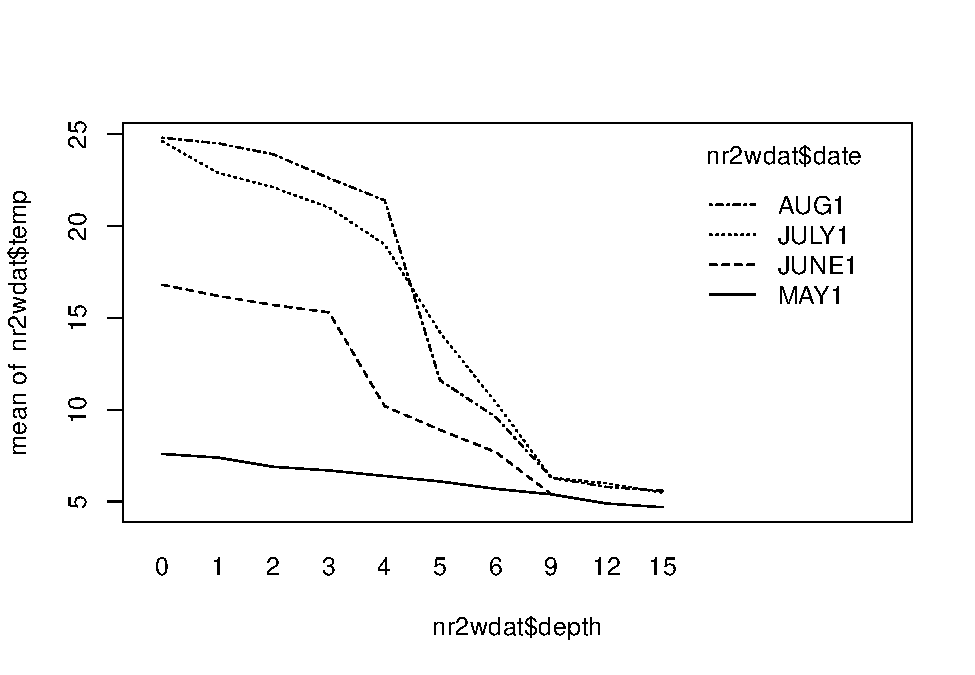
\includegraphics{Labs_BIO4158_files/figure-latex/unnamed-chunk-63-1.pdf}
\caption{\label{fig:unnamed-chunk-63}Effet du mois et de la profondeur sur la température}
\end{figure}

There is a highly significant decrease in temperature as depth increases. To test the effect of month (the (assumed) random factor), we must assume that there is no interaction between depth and month, i.e.~that the change in temperature with depth is the same for each month. This is a dubious assumption: if you plot temperature against depth for each month, you should see that the temperature profile becomes increasingly non-linear as the summer progresses (i.e.~the thermocline develops), from almost a linear decline in early spring to what amounts to a step decline in August. In other words, the relationship between temperature and depth does change with month, so that if you were to use the above fitted model to estimate, say, the temperature at a depth of 5 m in July, you would not get a particularly good estimate.

In terms of residual diagnostics, have a look at the residuals probability plot and residuals vs fitted values plot.

\begin{Shaded}
\begin{Highlighting}[]
\KeywordTok{par}\NormalTok{(}\DataTypeTok{mfrow =} \KeywordTok{c}\NormalTok{(}\DecValTok{2}\NormalTok{, }\DecValTok{2}\NormalTok{))}
\KeywordTok{plot}\NormalTok{(anova.model4)}
\end{Highlighting}
\end{Shaded}

\begin{verbatim}
## Error in xy.coords(x, y, xlabel, ylabel, log): 'x' and 'y' lengths differ
\end{verbatim}

\begin{figure}
\centering
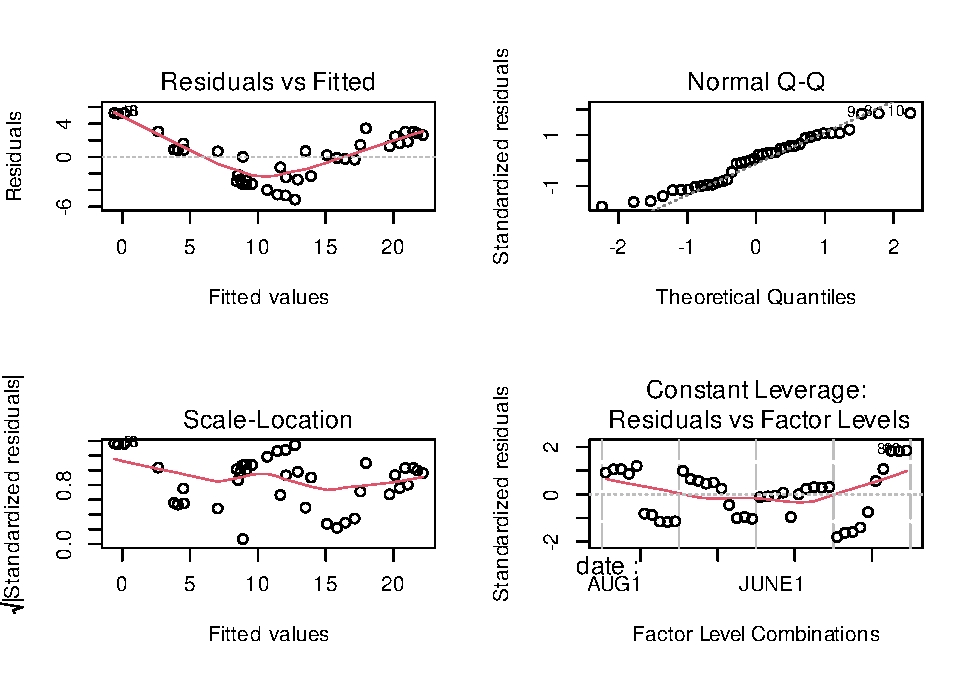
\includegraphics{Labs_BIO4158_files/figure-latex/unnamed-chunk-64-1.pdf}
\caption{\label{fig:unnamed-chunk-64}Conditions d'applications du modèle anova.model4}
\end{figure}

\begin{Shaded}
\begin{Highlighting}[]
\KeywordTok{shapiro.test}\NormalTok{(}\KeywordTok{residuals}\NormalTok{(anova.model4))}
\end{Highlighting}
\end{Shaded}

\begin{verbatim}
## 
##  Shapiro-Wilk normality test
## 
## data:  residuals(anova.model4)
## W = 0.95968, p-value = 0.1634
\end{verbatim}

Testing the residuals for normality, we get \texttt{p\ =\ 0.16}, so that the normality assumption seems to be O.K. In terms of heteroscedasticity, we can only test among months, using depths as replicates (or among depths using months as replicates). Using depths as replicates within months, we find

\begin{Shaded}
\begin{Highlighting}[]
\KeywordTok{leveneTest}\NormalTok{(temp }\OperatorTok{\textasciitilde{}}\StringTok{ }\NormalTok{date, }\DataTypeTok{data =}\NormalTok{ nr2wdat)}
\end{Highlighting}
\end{Shaded}

\begin{verbatim}
## Warning in leveneTest.default(y = y, group = group, ...): group coerced to
## factor.
\end{verbatim}

\begin{verbatim}
## Levene's Test for Homogeneity of Variance (center = median)
##       Df F value    Pr(>F)    
## group  3  17.979 2.679e-07 ***
##       36                      
## ---
## Signif. codes:  0 '***' 0.001 '**' 0.01 '*' 0.05 '.' 0.1 ' ' 1
\end{verbatim}

So there seems to be some problem here, as can be plainly seen in the above plot of residuals vs fit. All in all, this analysis is not very satisfactory: there appears to be some problems with the assumptions, and the assumption of no interaction between depth and date would appear to be invalid.

\hypertarget{nested-designs}{%
\section{Nested designs}\label{nested-designs}}

A common experimental design occurs when each major group (or treatment) is divided into randomly chosen subgroups. For example, a geneticist interested in the effects of genotype on desiccation resistance in fruit flies might conduct an experiment with larvae of three different genotypes. For each genotype (major group), she sets up three environmental chambers (sub-groups, replicates within groups) with a fixed temperature humidity regime, and in each chamber, she has five larvae for which she records the number of hours each larvae survived.

\begin{itemize}
\tightlist
\item
  The file \texttt{Nestdat.csv} contains the results of just such an experi ment. The file lists three variables: genotype , chamber and survival . Run a nested ANOVA with survival as the dependent variable, genotype/chamber as the independent variables (this is the shorthand notation for a chamber effect nested under genotype).
\end{itemize}

\begin{Shaded}
\begin{Highlighting}[]
\NormalTok{nestdat \textless{}{-}}\StringTok{ }\KeywordTok{read.csv}\NormalTok{(}\StringTok{"data/nestdat.csv"}\NormalTok{)}
\NormalTok{nestdat}\OperatorTok{$}\NormalTok{chamber \textless{}{-}}\StringTok{ }\KeywordTok{as.factor}\NormalTok{(nestdat}\OperatorTok{$}\NormalTok{chamber)}
\NormalTok{nestdat}\OperatorTok{$}\NormalTok{genotype \textless{}{-}}\StringTok{ }\KeywordTok{as.factor}\NormalTok{(nestdat}\OperatorTok{$}\NormalTok{genotype)}
\NormalTok{anova.nested \textless{}{-}}\StringTok{ }\KeywordTok{lm}\NormalTok{(survival }\OperatorTok{\textasciitilde{}}\StringTok{ }\NormalTok{genotype }\OperatorTok{/}\StringTok{ }\NormalTok{chamber, }\DataTypeTok{data =}\NormalTok{ nestdat)}
\end{Highlighting}
\end{Shaded}

What do you conclude from this analysis? What analysis would (should) you do next? (Hint: if there is a non-significant effect of chambers within genotypes, then you can increase the power of between-genotype comparisons by pooling over chambers within genotypes, although not everyone (Dr.~Rundle included) agrees with such pooling.) Do it! Make sure you check your assumptions!

\begin{verbatim}
## Analysis of Variance Table
## 
## Response: survival
##                  Df  Sum Sq Mean Sq  F value Pr(>F)    
## genotype          2 2952.22 1476.11 292.6081 <2e-16 ***
## genotype:chamber  6   40.65    6.78   1.3432 0.2639    
## Residuals        36  181.61    5.04                    
## ---
## Signif. codes:  0 '***' 0.001 '**' 0.01 '*' 0.05 '.' 0.1 ' ' 1
\end{verbatim}

\begin{figure}
\centering
\includegraphics{Labs_BIO4158_files/figure-latex/unnamed-chunk-68-1.pdf}
\caption{\label{fig:unnamed-chunk-68}Conditions d'applications du modèle anova.nested}
\end{figure}

We conclude from this analysis that there is no (significant) variation among chambers within genotypes, but that the null hypothesis that all genotypes have the same dessiccation resistance (as measured by survival) is rejected (Test of genotype using MS genotype:chamber as denominator: F = 1476.11/6.78 = 217.7153, P\textless0.0001). In other words, genotypes differ in their survival.

Since the chambers within genotypes effect is non-significant, we may want to pool over chambers to increase our degrees of freedom:

\begin{Shaded}
\begin{Highlighting}[]
\NormalTok{anova.simple \textless{}{-}}\StringTok{ }\KeywordTok{lm}\NormalTok{(survival }\OperatorTok{\textasciitilde{}}\StringTok{ }\NormalTok{genotype, }\DataTypeTok{data =}\NormalTok{ nestdat)}
\KeywordTok{anova}\NormalTok{(anova.simple)}
\end{Highlighting}
\end{Shaded}

\begin{verbatim}
## Analysis of Variance Table
## 
## Response: survival
##           Df  Sum Sq Mean Sq F value    Pr(>F)    
## genotype   2 2952.22 1476.11  278.93 < 2.2e-16 ***
## Residuals 42  222.26    5.29                      
## ---
## Signif. codes:  0 '***' 0.001 '**' 0.01 '*' 0.05 '.' 0.1 ' ' 1
\end{verbatim}

Thus, we conclude that there is significant variation among the three genotypes in dessiccation resistance.

A box plot of survival across genotypes shows clearly that there is significant variation among the three genotypes in dessiccation resistance. This can be combined with a formal Tukey multiple comparison test:

\begin{Shaded}
\begin{Highlighting}[]
\KeywordTok{par}\NormalTok{(}\DataTypeTok{mfrow =} \KeywordTok{c}\NormalTok{(}\DecValTok{1}\NormalTok{, }\DecValTok{1}\NormalTok{))}
\CommentTok{\# Compute and plot means and Tukey CI}
\NormalTok{means \textless{}{-}}\StringTok{ }\KeywordTok{glht}\NormalTok{(anova.simple, }\DataTypeTok{linfct =} \KeywordTok{mcp}\NormalTok{(}
  \DataTypeTok{genotype =}
    \StringTok{"Tukey"}
\NormalTok{))}
\NormalTok{cimeans \textless{}{-}}\StringTok{ }\KeywordTok{cld}\NormalTok{(means)}
\CommentTok{\# use sufficiently large upper margin}
\NormalTok{old.par \textless{}{-}}\StringTok{ }\KeywordTok{par}\NormalTok{(}\DataTypeTok{mai =} \KeywordTok{c}\NormalTok{(}\DecValTok{1}\NormalTok{, }\DecValTok{1}\NormalTok{, }\FloatTok{1.25}\NormalTok{, }\DecValTok{1}\NormalTok{))}
\CommentTok{\# plot}
\KeywordTok{plot}\NormalTok{(cimeans, }\DataTypeTok{las =} \DecValTok{1}\NormalTok{) }\CommentTok{\# las option to put y{-}axis labels as God intended them}
\end{Highlighting}
\end{Shaded}

\begin{figure}
\centering
\includegraphics{Labs_BIO4158_files/figure-latex/unnamed-chunk-70-1.pdf}
\caption{\label{fig:unnamed-chunk-70}Effet du genotype sur la résistance à la dessication avec un test de Tukey}
\end{figure}

So, we conclude from the Tukey analysis and plot that dessiccation resistance (R) , as measured by larval survival under hot, dry conditions, varies significantly among all three genotypes with R(AA) \textgreater{} R(Aa) \textgreater{} R(aa).

Before concluding this, however, we must test the assumptions. Here are the residual plots and diagnostics for the one-way (unnested) design:

\begin{figure}
\centering
\includegraphics{Labs_BIO4158_files/figure-latex/unnamed-chunk-71-1.pdf}
\caption{\label{fig:unnamed-chunk-71}Conditions d'applications du modèle anova.simple}
\end{figure}

So, all the assumptions appear to be valid, and the conclusion reached above still holds. Note that if you compare the residual mean squares of the nested and one-way ANOVAs (5.04 vs 5.29), they are almost identical. This is not surprising, given the small contribution of the chamber \%in\% genotype effect to the explained sum of squares.

\hypertarget{two-way-non-parametric-anova}{%
\section{Two-way non-parametric ANOVA}\label{two-way-non-parametric-anova}}

Two-way non-parametric ANOVA is an extension of the non-parametric one-way methods discussed previously. The basic procedure is to rank all the data in the sample from smallest to largest, then carry out a 2-way ANOVA on the ranks. This can be done either for replicated or unreplicated data.

Using the data file \texttt{Stu2wdat.csv} , do a two-factor ANOVA to examine the effects of \texttt{sex} and \texttt{location} on \texttt{rank(rdwght)}.

\begin{Shaded}
\begin{Highlighting}[]
\NormalTok{aov.rank \textless{}{-}}\StringTok{ }\KeywordTok{aov}\NormalTok{(}
  \KeywordTok{rank}\NormalTok{(rdwght) }\OperatorTok{\textasciitilde{}}\StringTok{ }\NormalTok{sex }\OperatorTok{*}\StringTok{ }\NormalTok{location,}
  \DataTypeTok{contrasts =} \KeywordTok{list}\NormalTok{(}
    \DataTypeTok{sex =}\NormalTok{ contr.sum, }\DataTypeTok{location =}\NormalTok{ contr.sum}
\NormalTok{  ),}
  \DataTypeTok{data =}\NormalTok{ Stu2wdat}
\NormalTok{)}
\end{Highlighting}
\end{Shaded}

The Scheirer-Ray-Hare extension of the Kruskall-Wallis test is done by computing a statistic H given by the effect sums of squares (SS) divided by the total MS. The latter can be calculated as the variance of the ranks. We compute an H statistic for each term. The H-statistics are then compared to a theoretical \(\chi^2\) (chi-square) distribution using the command line: \texttt{pchisq(H,\ df,\ lower.tail\ =\ FALSE)} , where \texttt{H} and \texttt{df} are the calculated H-statistics and associated degrees of freedom, respectively.

\begin{itemize}
\tightlist
\item
  Use the ANOVA table based on ranks to test the effects of \texttt{sex} and on \texttt{rdwght}. What do you conclude? How does this result compare with the result obtained with the parametric 2-way ANOVA done before?
\end{itemize}

\begin{Shaded}
\begin{Highlighting}[]
\KeywordTok{Anova}\NormalTok{(aov.rank, }\DataTypeTok{type =} \DecValTok{3}\NormalTok{)}
\end{Highlighting}
\end{Shaded}

\begin{verbatim}
## Anova Table (Type III tests)
## 
## Response: rank(rdwght)
##               Sum Sq  Df  F value    Pr(>F)    
## (Intercept)  1499862   1 577.8673 < 2.2e-16 ***
## sex            58394   1  22.4979 4.237e-06 ***
## location        1128   1   0.4347    0.5105    
## sex:location    1230   1   0.4738    0.4921    
## Residuals     472383 182                       
## ---
## Signif. codes:  0 '***' 0.001 '**' 0.01 '*' 0.05 '.' 0.1 ' ' 1
\end{verbatim}

To calculate the Scheirer-Ray-Hare extension to the Kruskall-Wallis test, you must first calculate the total mean square (MS), i.e.~the variance of the ranked data. In this case, there are 186 observations, their ranks are therefore the series 1, 2, 3, \ldots, 186. The variance can be calculated simply as var(1:186) (Isn't R neat? Cryptic maybe, but neat). So we can compute the \texttt{H} statistic for each term:

\begin{Shaded}
\begin{Highlighting}[]
\NormalTok{Hsex \textless{}{-}}\StringTok{ }\DecValTok{58394} \OperatorTok{/}\StringTok{ }\KeywordTok{var}\NormalTok{(}\DecValTok{1}\OperatorTok{:}\DecValTok{186}\NormalTok{)}
\NormalTok{Hlocation \textless{}{-}}\StringTok{ }\DecValTok{1128} \OperatorTok{/}\StringTok{ }\KeywordTok{var}\NormalTok{(}\DecValTok{1}\OperatorTok{:}\DecValTok{186}\NormalTok{)}
\NormalTok{Hsexloc \textless{}{-}}\StringTok{ }\DecValTok{1230} \OperatorTok{/}\StringTok{ }\KeywordTok{var}\NormalTok{(}\DecValTok{1}\OperatorTok{:}\DecValTok{186}\NormalTok{)}
\end{Highlighting}
\end{Shaded}

And convert these statistics into p-values:

\begin{Shaded}
\begin{Highlighting}[]
\CommentTok{\# sex}
\NormalTok{Hsex}
\end{Highlighting}
\end{Shaded}

\begin{verbatim}
## [1] 20.14628
\end{verbatim}

\begin{Shaded}
\begin{Highlighting}[]
\KeywordTok{pchisq}\NormalTok{(Hsex, }\DecValTok{1}\NormalTok{, }\DataTypeTok{lower.tail =} \OtherTok{FALSE}\NormalTok{)}
\end{Highlighting}
\end{Shaded}

\begin{verbatim}
## [1] 7.173954e-06
\end{verbatim}

\begin{Shaded}
\begin{Highlighting}[]
\CommentTok{\# location}
\NormalTok{Hlocation}
\end{Highlighting}
\end{Shaded}

\begin{verbatim}
## [1] 0.3891668
\end{verbatim}

\begin{Shaded}
\begin{Highlighting}[]
\KeywordTok{pchisq}\NormalTok{(Hlocation, }\DecValTok{1}\NormalTok{, }\DataTypeTok{lower.tail =} \OtherTok{FALSE}\NormalTok{)}
\end{Highlighting}
\end{Shaded}

\begin{verbatim}
## [1] 0.5327377
\end{verbatim}

\begin{Shaded}
\begin{Highlighting}[]
\CommentTok{\# sex:location}
\NormalTok{Hsexloc}
\end{Highlighting}
\end{Shaded}

\begin{verbatim}
## [1] 0.4243574
\end{verbatim}

\begin{Shaded}
\begin{Highlighting}[]
\KeywordTok{pchisq}\NormalTok{(Hsexloc, }\DecValTok{1}\NormalTok{, }\DataTypeTok{lower.tail =} \OtherTok{FALSE}\NormalTok{)}
\end{Highlighting}
\end{Shaded}

\begin{verbatim}
## [1] 0.5147707
\end{verbatim}

Note that these results are the same as those obtained in our original two-way parametric ANOVA. Despite the reduced power, we still find significant differences between the sexes, but still no interaction and no effect due to location.

There is, however, an important difference. Recall that in the original parametric ANOVA, there was a significant effect of sex when we considered the problem as a Model I ANOVA. However, if we consider it as Model III, the significant sex effect could in principle disappear, because the df associated with the interaction MS are much smaller than the df associated with the Model I error MS. In this case, however, the interaction MS is about half that of the error MS. So, the significant sex effect becomes even more significant if we analyze the problem as a Model III ANOVA. Once again, we see the importance of specifying the appropriate ANOVA design.

\hypertarget{multiple-comparisons}{%
\section{Multiple comparisons}\label{multiple-comparisons}}

Further hypothesis testing in multiway ANOVAs depends critically on the outcome of the initial ANOVA. If you are interested in comparing groups of marginal means (that is, means of treatments for one factor pooled over levels of the other factor, e.g., between male and female sturgeon pooled over location), this can be done exactly as outlined for multiple comparisons for one-way ANOVAs. For comparison of individual cell means, you must specify the interaction as the group variable.

The file \texttt{wmcdat2.csv} shows measured oxygen consumption ( \texttt{o2cons} ) of two species ( \texttt{species} = A, B)) of limpets at three different concentrations of seawater ( \texttt{conc} = 100, 75, 50\%) taken from Sokal and Rohlf, 1995, p.~332.

\begin{itemize}
\tightlist
\item
  Run a 2-way factorial ANOVA on \texttt{wmcdat2} data, using \texttt{o2cons} as the dependent variable and species and conc as the factors. What do you conclude?
\end{itemize}

The ANOVA table is shown below. Technically, because the sample sizes in individual cells are rather small, this analysis should be repeated using a non-parametric ANOVA. For the moment, let's stick with the parametric analysis.

\begin{verbatim}
## Anova Table (Type III tests)
## 
## Response: o2cons
##               Sum Sq Df  F value    Pr(>F)    
## (Intercept)  1185.60  1 124.0165 4.101e-14 ***
## species         0.09  1   0.0097   0.92189    
## conc           74.90  2   3.9172   0.02755 *  
## species:conc   23.93  2   1.2514   0.29656    
## Residuals     401.52 42                       
## ---
## Signif. codes:  0 '***' 0.001 '**' 0.01 '*' 0.05 '.' 0.1 ' ' 1
\end{verbatim}

Look at the diagnostic plots:

\includegraphics{Labs_BIO4158_files/figure-latex/unnamed-chunk-78-1.pdf}

Homoscedasticity looks ok, but normality less so.. Testing for
normality, we get:

\begin{verbatim}
## 
##  Shapiro-Wilk normality test
## 
## data:  residuals(anova.model5)
## W = 0.93692, p-value = 0.01238
\end{verbatim}

So there is evidence of non-normality, but otherwise everything looks O.K. Since the ANOVA is relatively robust with respect to non-normality, we proceed, but if we wanted to reassure ourselves, we could run a non-parametric ANOVA, and get the same answer.

\begin{itemize}
\tightlist
\item
  On the basis of the ANOVA results obtained above, which means would you proceed to compare? Why?
\end{itemize}

Overall, we conclude that there are no differences among species, and that the effect of concentration does not depend on species (no interaction). Since there is no interaction and no main effect due to species, the only comparison of interest is among salinity concentrations:

\begin{Shaded}
\begin{Highlighting}[]
\CommentTok{\# fit simplified model}
\NormalTok{anova.model6 \textless{}{-}}\StringTok{ }\KeywordTok{aov}\NormalTok{(o2cons }\OperatorTok{\textasciitilde{}}\StringTok{ }\NormalTok{conc, }\DataTypeTok{data =}\NormalTok{ wmcdat2)}
\CommentTok{\# Make Tukey multiple comparisons}
\KeywordTok{TukeyHSD}\NormalTok{(anova.model6)}
\end{Highlighting}
\end{Shaded}

\begin{verbatim}
##   Tukey multiple comparisons of means
##     95% family-wise confidence level
## 
## Fit: aov(formula = o2cons ~ conc, data = wmcdat2)
## 
## $conc
##            diff       lwr        upr     p adj
## 75-50  -4.63625 -7.321998 -1.9505018 0.0003793
## 100-50 -3.25500 -5.940748 -0.5692518 0.0141313
## 100-75  1.38125 -1.304498  4.0669982 0.4325855
\end{verbatim}

\begin{Shaded}
\begin{Highlighting}[]
\KeywordTok{par}\NormalTok{(}\DataTypeTok{mfrow =} \KeywordTok{c}\NormalTok{(}\DecValTok{1}\NormalTok{, }\DecValTok{1}\NormalTok{))}
\CommentTok{\# Graph of all comparisons for conc}
\NormalTok{tuk \textless{}{-}}\StringTok{ }\KeywordTok{glht}\NormalTok{(anova.model6, }\DataTypeTok{linfct =} \KeywordTok{mcp}\NormalTok{(}\DataTypeTok{conc =} \StringTok{"Tukey"}\NormalTok{))}
\CommentTok{\# extract information}
\NormalTok{tuk.cld \textless{}{-}}\StringTok{ }\KeywordTok{cld}\NormalTok{(tuk)}
\CommentTok{\# use sufficiently large upper margin}
\NormalTok{old.par \textless{}{-}}\StringTok{ }\KeywordTok{par}\NormalTok{(}\DataTypeTok{mai =} \KeywordTok{c}\NormalTok{(}\DecValTok{1}\NormalTok{, }\DecValTok{1}\NormalTok{, }\FloatTok{1.25}\NormalTok{, }\DecValTok{1}\NormalTok{))}
\CommentTok{\# plot}
\KeywordTok{plot}\NormalTok{(tuk.cld)}
\end{Highlighting}
\end{Shaded}

\begin{figure}
\centering
\includegraphics{Labs_BIO4158_files/figure-latex/unnamed-chunk-81-1.pdf}
\caption{\label{fig:unnamed-chunk-81}Comparaison de Tukey des moyennes de consommation d'oxygèn en fonction del la concentration}
\end{figure}

\begin{Shaded}
\begin{Highlighting}[]
\KeywordTok{par}\NormalTok{(old.par)}
\end{Highlighting}
\end{Shaded}

So there is evidence of a significant difference in oxygen consumption at a reduction in salinity to 50\% of regular seawater, but not at a reduction of only 25\%.

\begin{itemize}
\tightlist
\item
  Repeat the analysis described above using \texttt{wmc2dat2.csv} . How do
  your results compare with those obtained for \texttt{wmcdat2.csv} ?
\end{itemize}

Using \texttt{wmc2dat2.csv},we get:

\begin{verbatim}
## Anova Table (Type III tests)
## 
## Response: o2cons
##              Sum Sq Df F value    Pr(>F)    
## (Intercept)  343.09  1 36.2132 3.745e-07 ***
## species      133.52  1 14.0929 0.0005286 ***
## conc          66.76  2  3.5232 0.0385011 *  
## species:conc 168.15  2  8.8742 0.0006101 ***
## Residuals    397.91 42                      
## ---
## Signif. codes:  0 '***' 0.001 '**' 0.01 '*' 0.05 '.' 0.1 ' ' 1
\end{verbatim}

Here there is a large interaction effect, and consequently, there is no
point in comparing marginal means. This is made clear by examining
an interaction plot:

\begin{Shaded}
\begin{Highlighting}[]
\KeywordTok{with}\NormalTok{(wmc2dat2, }\KeywordTok{interaction.plot}\NormalTok{(conc, species, o2cons))}
\end{Highlighting}
\end{Shaded}

\includegraphics{Labs_BIO4158_files/figure-latex/unnamed-chunk-84-1.pdf}

\begin{itemize}
\tightlist
\item
  Working still with the \texttt{wmc2dat2} data set, compare individual cell means (6 in all), with the Bonferonni adjustment. To do this, it is helpful to create a new variable to indicate all the combinations of \texttt{species} and \texttt{conc}:
\end{itemize}

\begin{Shaded}
\begin{Highlighting}[]
\NormalTok{wmc2dat2}\OperatorTok{$}\NormalTok{species.conc \textless{}{-}}\StringTok{ }\KeywordTok{as.factor}\NormalTok{(}\KeywordTok{paste0}\NormalTok{(wmc2dat2}\OperatorTok{$}\NormalTok{species, wmc2dat2}\OperatorTok{$}\NormalTok{conc))}
\end{Highlighting}
\end{Shaded}

Then we can conduct pairwise bonferroni comparisons:

\begin{Shaded}
\begin{Highlighting}[]
\KeywordTok{with}\NormalTok{(wmc2dat2, }\KeywordTok{pairwise.t.test}\NormalTok{(o2cons, species.conc, }\DataTypeTok{p.adj =} \StringTok{"bonf"}\NormalTok{))}
\end{Highlighting}
\end{Shaded}

\begin{verbatim}
## 
##  Pairwise comparisons using t tests with pooled SD 
## 
## data:  o2cons and species.conc 
## 
##      A100   A50    A75    B100   B50   
## A50  0.1887 -      -      -      -     
## A75  1.0000 1.0000 -      -      -     
## B100 0.7223 1.0000 1.0000 -      -     
## B50  1.0000 0.0079 0.0929 0.0412 -     
## B75  0.6340 1.0000 1.0000 1.0000 0.0350
## 
## P value adjustment method: bonferroni
\end{verbatim}

These comparisons are a little more difficult to interpret, but the analysis essentially examines for differences among seawater concentrations within species A and for differences among concentrations within species B. We see here that the o2Cons at 50\% seawater for species B is significantly different from that of 75\% and 100\% seawater for species B, whereas there are no significant differences in \texttt{o2cons} for species A across all seawater concentrations.

I find these outputs rather unsatisfying because they show only p- values, but no indication of effect size. One can get both the conclusion from the multiple comparison procedure and an indication of effect size from the graph produced with the following code:

\begin{Shaded}
\begin{Highlighting}[]
\CommentTok{\# fit one{-}way anova comparing all combinations of species.conc combinations}
\NormalTok{anova.modelx \textless{}{-}}\StringTok{ }\KeywordTok{aov}\NormalTok{(o2cons }\OperatorTok{\textasciitilde{}}\StringTok{ }\NormalTok{species.conc, }\DataTypeTok{data =}\NormalTok{ wmc2dat2)}
\NormalTok{tuk2 \textless{}{-}}\StringTok{ }\KeywordTok{glht}\NormalTok{(anova.modelx, }\DataTypeTok{linfct =} \KeywordTok{mcp}\NormalTok{(}\DataTypeTok{species.conc =} \StringTok{"Tukey"}\NormalTok{))}
\CommentTok{\# extract information}
\NormalTok{tuk2.cld \textless{}{-}}\StringTok{ }\KeywordTok{cld}\NormalTok{(tuk2)}
\CommentTok{\# use sufficiently large upper margin}
\NormalTok{old.par \textless{}{-}}\StringTok{ }\KeywordTok{par}\NormalTok{(}\DataTypeTok{mai =} \KeywordTok{c}\NormalTok{(}\DecValTok{1}\NormalTok{, }\DecValTok{1}\NormalTok{, }\FloatTok{1.25}\NormalTok{, }\DecValTok{1}\NormalTok{))}
\CommentTok{\# plot}
\KeywordTok{plot}\NormalTok{(tuk2.cld)}
\end{Highlighting}
\end{Shaded}

\includegraphics{Labs_BIO4158_files/figure-latex/unnamed-chunk-87-1.pdf}

\begin{Shaded}
\begin{Highlighting}[]
\KeywordTok{par}\NormalTok{(old.par)}
\end{Highlighting}
\end{Shaded}

Note that in this analysis, we have used the error MS = 9.474 from the original model to contrast cell means. Recall, however, that this assumes that in fact we are dealing with a Model I ANOVA, which may or may not be the case ( conc is certainly a fixed factor, but species might be either fixed or random).

\hypertarget{test-de-permutation-pour-lanova-uxe0-deux-facteurs-de-classification}{%
\section{Test de permutation pour l'ANOVA à deux facteurs de classification}\label{test-de-permutation-pour-lanova-uxe0-deux-facteurs-de-classification}}

When data do not meet the assumptions of the parametric analysis in two- and multiway ANOVA, as an alternative to the non-parametric ANOVA, , it is possible to run permutation tests to calculate p- values. The lmPerm package does this easily.

\begin{Shaded}
\begin{Highlighting}[]
\CommentTok{\#\#\#\#\#\#\#\#\#\#\#\#\#\#\#\#\#\#\#\#\#\#\#\#\#\#\#\#\#\#\#\#\#\#\#\#\#\#\#\#\#\#\#\#\#\#\#\#\#\#\#\#\#\#\#\#\#\#\#\#\#\#\#\#\#\#\#\#\#\#\#}
\CommentTok{\#\# lmPerm version of permutation test}
\KeywordTok{library}\NormalTok{(lmPerm)}
\CommentTok{\# for generality, copy desired dataframe to mydata}
\CommentTok{\# and model formula to myformula}
\NormalTok{mydata \textless{}{-}}\StringTok{ }\NormalTok{Stu2wdat}
\NormalTok{myformula \textless{}{-}}\StringTok{ }\KeywordTok{as.formula}\NormalTok{(}\StringTok{"rdwght \textasciitilde{} sex+location+sex:location"}\NormalTok{)}
\CommentTok{\# Fit desired model on the desired dataframe}
\NormalTok{mymodel \textless{}{-}}\StringTok{ }\KeywordTok{lm}\NormalTok{(myformula, }\DataTypeTok{data =}\NormalTok{ mydata)}
\CommentTok{\# Calculate permutation p{-}value}
\KeywordTok{anova}\NormalTok{(}\KeywordTok{lmp}\NormalTok{(myformula, }\DataTypeTok{data =}\NormalTok{ mydata, }\DataTypeTok{perm =} \StringTok{"Prob"}\NormalTok{, }\DataTypeTok{center =} \OtherTok{FALSE}\NormalTok{, }\DataTypeTok{Ca =} \FloatTok{0.001}\NormalTok{))}
\end{Highlighting}
\end{Shaded}

\texttt{lmPerm} was orphaned for a while and the code below, while clunkier, provided an alternative way of doing it. You would have to adapt it for other situations.

\begin{Shaded}
\begin{Highlighting}[]
\CommentTok{\#\#\#\#\#\#\#\#\#\#\#\#\#\#\#\#\#\#\#\#\#\#\#\#\#\#\#\#\#\#\#\#\#\#\#\#\#\#\#\#\#\#\#\#\#\#\#\#\#\#\#\#\#\#\#\#\#\#\#}
\CommentTok{\# Permutation test for two way ANOVA}
\CommentTok{\# Ter Braak creates residuals from cell means and then permutes across}
\CommentTok{\# all cells}
\CommentTok{\# This can be accomplished by taking residuals from the full model}
\CommentTok{\# modified from code written by David C. Howell}
\CommentTok{\# http://www.uvm.edu/\textasciitilde{}dhowell/StatPages/More\_Stuff/Permutation\%20Anova/PermTestsAnova.html}
\NormalTok{nreps \textless{}{-}}\StringTok{ }\DecValTok{500}
\NormalTok{dependent \textless{}{-}}\StringTok{ }\NormalTok{Stu2wdat}\OperatorTok{$}\NormalTok{rdwght}
\NormalTok{factor1 \textless{}{-}}\StringTok{ }\KeywordTok{as.factor}\NormalTok{(Stu2wdat}\OperatorTok{$}\NormalTok{sex)}
\NormalTok{factor2 \textless{}{-}}\StringTok{ }\KeywordTok{as.factor}\NormalTok{(Stu2wdat}\OperatorTok{$}\NormalTok{location)}
\NormalTok{my.dataframe \textless{}{-}}\StringTok{ }\KeywordTok{data.frame}\NormalTok{(dependent, factor1, factor2)}
\NormalTok{my.dataframe.noNA \textless{}{-}}\StringTok{ }\NormalTok{my.dataframe[}\KeywordTok{complete.cases}\NormalTok{(my.dataframe), ]}
\NormalTok{mod \textless{}{-}}\StringTok{ }\KeywordTok{lm}\NormalTok{(dependent }\OperatorTok{\textasciitilde{}}\StringTok{ }\NormalTok{factor1 }\OperatorTok{+}\StringTok{ }\NormalTok{factor2 }\OperatorTok{+}\StringTok{ }\NormalTok{factor1}\OperatorTok{:}\NormalTok{factor2,}
  \DataTypeTok{data =}\NormalTok{ my.dataframe.noNA}
\NormalTok{)}
\NormalTok{res \textless{}{-}}\StringTok{ }\NormalTok{mod}\OperatorTok{$}\NormalTok{residuals}
\NormalTok{TBint \textless{}{-}}\StringTok{ }\KeywordTok{numeric}\NormalTok{(nreps)}
\NormalTok{TB1 \textless{}{-}}\StringTok{ }\KeywordTok{numeric}\NormalTok{(nreps)}
\NormalTok{TB2 \textless{}{-}}\StringTok{ }\KeywordTok{numeric}\NormalTok{(nreps)}
\NormalTok{ANOVA \textless{}{-}}\StringTok{ }\KeywordTok{summary}\NormalTok{(}\KeywordTok{aov}\NormalTok{(mod))}
\KeywordTok{cat}\NormalTok{(}
  \StringTok{" The standard ANOVA for these data follows "}\NormalTok{,}
  \StringTok{"}\CharTok{\textbackslash{}n}\StringTok{"}
\NormalTok{)}
\NormalTok{F1 \textless{}{-}}\StringTok{ }\NormalTok{ANOVA[[}\DecValTok{1}\NormalTok{]]}\OperatorTok{$}\StringTok{"F value"}\NormalTok{[}\DecValTok{1}\NormalTok{]}
\NormalTok{F2 \textless{}{-}}\StringTok{ }\NormalTok{ANOVA[[}\DecValTok{1}\NormalTok{]]}\OperatorTok{$}\StringTok{"F value"}\NormalTok{[}\DecValTok{2}\NormalTok{]}
\NormalTok{Finteract \textless{}{-}}\StringTok{ }\NormalTok{ANOVA[[}\DecValTok{1}\NormalTok{]]}\OperatorTok{$}\StringTok{"F value"}\NormalTok{[}\DecValTok{3}\NormalTok{]}
\KeywordTok{print}\NormalTok{(ANOVA)}
\KeywordTok{cat}\NormalTok{(}\StringTok{"}\CharTok{\textbackslash{}n}\StringTok{"}\NormalTok{)}
\KeywordTok{cat}\NormalTok{(}\StringTok{"}\CharTok{\textbackslash{}n}\StringTok{"}\NormalTok{)}
\NormalTok{TBint[}\DecValTok{1}\NormalTok{] \textless{}{-}}\StringTok{ }\NormalTok{Finteract}
\ControlFlowTok{for}\NormalTok{ (i }\ControlFlowTok{in} \DecValTok{2}\OperatorTok{:}\NormalTok{nreps) \{}
\NormalTok{  newdat \textless{}{-}}\StringTok{ }\KeywordTok{sample}\NormalTok{(res, }\KeywordTok{length}\NormalTok{(res), }\DataTypeTok{replace =} \OtherTok{FALSE}\NormalTok{)}
\NormalTok{  modb \textless{}{-}}\StringTok{ }\KeywordTok{summary}\NormalTok{(}\KeywordTok{aov}\NormalTok{(newdat }\OperatorTok{\textasciitilde{}}\StringTok{ }\NormalTok{factor1 }\OperatorTok{+}\StringTok{ }\NormalTok{factor2 }\OperatorTok{+}
\StringTok{    }\NormalTok{factor1}\OperatorTok{:}\NormalTok{factor2,}
  \DataTypeTok{data =}\NormalTok{ my.dataframe.noNA}
\NormalTok{  ))}
\NormalTok{  TBint[i] \textless{}{-}}\StringTok{ }\NormalTok{modb[[}\DecValTok{1}\NormalTok{]]}\OperatorTok{$}\StringTok{"F value"}\NormalTok{[}\DecValTok{3}\NormalTok{]}
\NormalTok{  TB1[i] \textless{}{-}}\StringTok{ }\NormalTok{modb[[}\DecValTok{1}\NormalTok{]]}\OperatorTok{$}\StringTok{"F value"}\NormalTok{[}\DecValTok{1}\NormalTok{]}
\NormalTok{  TB2[i] \textless{}{-}}\StringTok{ }\NormalTok{modb[[}\DecValTok{1}\NormalTok{]]}\OperatorTok{$}\StringTok{"F value"}\NormalTok{[}\DecValTok{2}\NormalTok{]}
\NormalTok{\}}
\NormalTok{probInt \textless{}{-}}\StringTok{ }\KeywordTok{length}\NormalTok{(TBint[TBint }\OperatorTok{\textgreater{}=}\StringTok{ }\NormalTok{Finteract]) }\OperatorTok{/}\StringTok{ }\NormalTok{nreps}
\NormalTok{prob1 \textless{}{-}}\StringTok{ }\KeywordTok{length}\NormalTok{(TB1[TB1 }\OperatorTok{\textgreater{}=}\StringTok{ }\NormalTok{F1]) }\OperatorTok{/}\StringTok{ }\NormalTok{nreps}
\NormalTok{prob2 \textless{}{-}}\StringTok{ }\KeywordTok{length}\NormalTok{(TB2[TB1 }\OperatorTok{\textgreater{}=}\StringTok{ }\NormalTok{F2]) }\OperatorTok{/}\StringTok{ }\NormalTok{nreps}
\KeywordTok{cat}\NormalTok{(}\StringTok{"}\CharTok{\textbackslash{}n}\StringTok{"}\NormalTok{)}
\KeywordTok{cat}\NormalTok{(}\StringTok{"}\CharTok{\textbackslash{}n}\StringTok{"}\NormalTok{)}
\KeywordTok{print}\NormalTok{(}\StringTok{"Resampling as in ter Braak with unrestricted sampling}
\StringTok{of cell residuals. "}\NormalTok{)}
\KeywordTok{cat}\NormalTok{(}
  \StringTok{"The probability for the effect of Interaction is "}\NormalTok{,}
\NormalTok{  probInt, }\StringTok{"}\CharTok{\textbackslash{}n}\StringTok{"}
\NormalTok{)}
\KeywordTok{cat}\NormalTok{(}
  \StringTok{"The probability for the effect of Factor 1 is "}\NormalTok{,}
\NormalTok{  prob1, }\StringTok{"}\CharTok{\textbackslash{}n}\StringTok{"}
\NormalTok{)}
\KeywordTok{cat}\NormalTok{(}
  \StringTok{"The probability for the effect of Factor 2 is "}\NormalTok{,}
\NormalTok{  prob2, }\StringTok{"}\CharTok{\textbackslash{}n}\StringTok{"}
\NormalTok{)}
\end{Highlighting}
\end{Shaded}

\hypertarget{bootstrap-for-two-way-anova}{%
\section{Bootstrap for two-way ANOVA}\label{bootstrap-for-two-way-anova}}

In most cases, permutation tests will be more appropriate than bootstrap in ANOVA designs. However, for the sake of completedness, I have a snippet of code to do bootstrap for you::

\begin{Shaded}
\begin{Highlighting}[]
\CommentTok{\#\#\#\#\#\#\#\#\#\#\#\#\#\#\#\#\#\#\#\#\#\#\#\#\#\#\#\#\#\#\#\#\#\#\#\#\#\#\#\#\#\#\#\#\#\#\#\#\#\#\#\#\#\#\#\#\#\#\#\#}
\CommentTok{\#\#\#\#\#\#\#\#\#\#\#}
\CommentTok{\# Bootstrap for two{-}way ANOVA}
\CommentTok{\# You possibly want to edit bootfunction.mod1 to return other values}
\CommentTok{\# Here it returns the standard coefficients of the fitted model}
\CommentTok{\# Requires boot library}
\CommentTok{\#}
\NormalTok{nreps \textless{}{-}}\StringTok{ }\DecValTok{5000}
\NormalTok{dependent \textless{}{-}}\StringTok{ }\NormalTok{Stu2wdat}\OperatorTok{$}\NormalTok{rdwght}
\NormalTok{factor1 \textless{}{-}}\StringTok{ }\KeywordTok{as.factor}\NormalTok{(Stu2wdat}\OperatorTok{$}\NormalTok{sex)}
\NormalTok{factor2 \textless{}{-}}\StringTok{ }\KeywordTok{as.factor}\NormalTok{(Stu2wdat}\OperatorTok{$}\NormalTok{location)}
\NormalTok{my.dataframe \textless{}{-}}\StringTok{ }\KeywordTok{data.frame}\NormalTok{(dependent, factor1, factor2)}
\NormalTok{my.dataframe.noNA \textless{}{-}}\StringTok{ }\NormalTok{my.dataframe[}\KeywordTok{complete.cases}\NormalTok{(my.dataframe), ]}
\KeywordTok{library}\NormalTok{(boot)}
\CommentTok{\# Fit model on observed data}
\NormalTok{mod1 \textless{}{-}}\StringTok{ }\KeywordTok{aov}\NormalTok{(dependent }\OperatorTok{\textasciitilde{}}\StringTok{ }\NormalTok{factor1 }\OperatorTok{+}\StringTok{ }\NormalTok{factor2 }\OperatorTok{+}\StringTok{ }\NormalTok{factor1}\OperatorTok{:}\NormalTok{factor2,}
  \DataTypeTok{data =}\NormalTok{ my.dataframe.noNA}
\NormalTok{)}


\CommentTok{\# Bootstrap 1000 time using the residuals bootstraping methods to}
\CommentTok{\# keep the same unequal number of observations for each level of the indep. var.}
\NormalTok{fit \textless{}{-}}\StringTok{ }\KeywordTok{fitted}\NormalTok{(mod1)}
\NormalTok{e \textless{}{-}}\StringTok{ }\KeywordTok{residuals}\NormalTok{(mod1)}
\NormalTok{X \textless{}{-}}\StringTok{ }\KeywordTok{model.matrix}\NormalTok{(mod1)}
\NormalTok{bootfunction.mod1 \textless{}{-}}\StringTok{ }\ControlFlowTok{function}\NormalTok{(data, indices) \{}
\NormalTok{  y \textless{}{-}}\StringTok{ }\NormalTok{fit }\OperatorTok{+}\StringTok{ }\NormalTok{e[indices]}
\NormalTok{  bootmod \textless{}{-}}\StringTok{ }\KeywordTok{lm}\NormalTok{(y }\OperatorTok{\textasciitilde{}}\StringTok{ }\NormalTok{X)}
  \KeywordTok{coefficients}\NormalTok{(bootmod)}
\NormalTok{\}}
\NormalTok{bootresults \textless{}{-}}\StringTok{ }\KeywordTok{boot}\NormalTok{(my.dataframe.noNA, bootfunction.mod1,}
  \DataTypeTok{R =} \DecValTok{1000}
\NormalTok{)}
\NormalTok{bootresults}
\CommentTok{\#\# Calculate 90\% CI and plot bootstrap estimates separately for each model parameter}
\KeywordTok{boot.ci}\NormalTok{(bootresults, }\DataTypeTok{conf =} \FloatTok{0.9}\NormalTok{, }\DataTypeTok{index =} \DecValTok{1}\NormalTok{)}
\KeywordTok{plot}\NormalTok{(bootresults, }\DataTypeTok{index =} \DecValTok{1}\NormalTok{)}
\KeywordTok{boot.ci}\NormalTok{(bootresults, }\DataTypeTok{conf =} \FloatTok{0.9}\NormalTok{, }\DataTypeTok{index =} \DecValTok{3}\NormalTok{)}
\KeywordTok{plot}\NormalTok{(bootresults, }\DataTypeTok{index =} \DecValTok{3}\NormalTok{)}
\KeywordTok{boot.ci}\NormalTok{(bootresults, }\DataTypeTok{conf =} \FloatTok{0.9}\NormalTok{, }\DataTypeTok{index =} \DecValTok{4}\NormalTok{)}
\KeywordTok{plot}\NormalTok{(bootresults, }\DataTypeTok{index =} \DecValTok{4}\NormalTok{)}
\KeywordTok{boot.ci}\NormalTok{(bootresults, }\DataTypeTok{conf =} \FloatTok{0.9}\NormalTok{, }\DataTypeTok{index =} \DecValTok{5}\NormalTok{)}
\KeywordTok{plot}\NormalTok{(bootresults, }\DataTypeTok{index =} \DecValTok{5}\NormalTok{)}
\end{Highlighting}
\end{Shaded}

\hypertarget{multiple-regression}{%
\chapter{Multiple regression}\label{multiple-regression}}

After completing this laboratory exercise, you should be able to:

\begin{itemize}
\tightlist
\item
  Use R to fit a multiple regression model, and compare the adequacy of several models using inferential and information theo-
  retic criteria
\item
  Use R to test hypotheses about the effects of different independent variables on the dependent variable of interest.
\item
  Use R to evaluate multicollinearity among (supposedly) independent variables and its effects.
\item
  Use R to do curvilinear (polynomial) regression.
\end{itemize}

\hypertarget{set-reg-mul}{%
\section{R packages and data}\label{set-reg-mul}}

For this lab you need:

\begin{itemize}
\tightlist
\item
  R packages:

  \begin{itemize}
  \tightlist
  \item
    ggplot2
  \item
    car
  \item
    lmtest
  \item
    simpleboot
  \item
    boot
  \item
    MuMIn
  \end{itemize}
\item
  data files:

  \begin{itemize}
  \tightlist
  \item
    Mregdat.csv
  \end{itemize}
\end{itemize}

\hypertarget{points-to-keep-in-mind}{%
\section{Points to keep in mind}\label{points-to-keep-in-mind}}

Multiple regression models are used in cases where there is one dependent variable and several independent, continuous variables. In many biological systems, the variable of interest may be influenced by several different factors, so that accurate description or prediction requires that several independent variables be included in the regression model. Before beginning, be aware that multiple regression takes time to learn well. Beginners should keep in mind several important points:

\begin{enumerate}
\def\labelenumi{\arabic{enumi}.}
\tightlist
\item
  An overall regression model may be statistically significant even if none of the individual regression coefficients in the model are (caused by multicollinearity)
\item
  A multiple regression model may be ``nonsignificant'' even though some of the individual coefficients are ``significant'' (caused by overfitting)
\item
  Unless ``independent'' variables are uncorrelated in the sample, different model selection procedures may yield different results.
\end{enumerate}

\hypertarget{first-look-at-the-data}{%
\section{First look at the data}\label{first-look-at-the-data}}

The file Mregdat.Rdata contains data collected in 30 wetlands in the Ottawa-Cornwall- Kingston area. The data included are

\begin{itemize}
\tightlist
\item
  the richness (number of species) of:

  \begin{itemize}
  \tightlist
  \item
    birds (\texttt{bird} , and its log transform \texttt{logbird}),
  \item
    plants (\texttt{plant}, \texttt{logpl}),
  \item
    mammals (\texttt{mammal}, \texttt{logmam}),
  \item
    herptiles (\texttt{herptile}, \texttt{logherp})
  \item
    total species richness of all four groups combined (\texttt{totsp}, \texttt{logtot})
  \end{itemize}
\item
  GPS coordinates of the wetland (\texttt{lat} , \texttt{long})
\item
  its area (\texttt{logarea})
\item
  the percentage of the wetland covered by water at all times during the year (\texttt{swamp})
\item
  the percentage of forested land within 1 km of the wetland (cpfor2)
\item
  the density (in m/hectare) of hard-surface roads within 1 km of the wetland (\texttt{thtden}).
\end{itemize}

We will focus on herptiles for this exercise, so we better first have a look at how this variable is distributed and correlated to the potential independent variables:

\begin{Shaded}
\begin{Highlighting}[]
\NormalTok{mydata \textless{}{-}}\StringTok{ }\KeywordTok{read.csv}\NormalTok{(}\StringTok{"data/Mregdat.csv"}\NormalTok{)}
\KeywordTok{scatterplotMatrix}\NormalTok{(}
  \OperatorTok{\textasciitilde{}}\StringTok{ }\NormalTok{logherp }\OperatorTok{+}\StringTok{ }\NormalTok{logarea }\OperatorTok{+}\StringTok{ }\NormalTok{cpfor2 }\OperatorTok{+}\StringTok{ }\NormalTok{thtden }\OperatorTok{+}\StringTok{ }\NormalTok{swamp,}
  \DataTypeTok{regLine =} \OtherTok{TRUE}\NormalTok{, }\DataTypeTok{smooth =} \OtherTok{TRUE}\NormalTok{, }\DataTypeTok{diagonal =} \OtherTok{TRUE}\NormalTok{,}
  \DataTypeTok{data =}\NormalTok{ mydata}
\NormalTok{)}
\end{Highlighting}
\end{Shaded}

\begin{figure}
\centering
\includegraphics{Labs_BIO4158_files/figure-latex/unnamed-chunk-88-1.pdf}
\caption{\label{fig:unnamed-chunk-88}Matrice de rélation et densité pour la richesse spécifique des amphibiens et reptiles}
\end{figure}

\hypertarget{multiple-regression-models-from-scratch}{%
\section{Multiple regression models from scratch}\label{multiple-regression-models-from-scratch}}

We begin the multiple regression exercise by considering a situation with one dependent variable and three (possibly) independent variables. First, we will start from scratch and build a multiple regression model based on what we know from building simple regression models. Next, we will look at automated methods of building multiple regressions models using simultaneous, forward, and backward stepwise procedures.

\begin{rmdcode}
Using the subset of the \texttt{Mregdat.csv} data file, regress \texttt{logherp} on \texttt{logarea}.
\end{rmdcode}

On the basis of the regression, what do you conclude?

\begin{Shaded}
\begin{Highlighting}[]
\NormalTok{model\_loga \textless{}{-}}\StringTok{ }\KeywordTok{lm}\NormalTok{(logherp }\OperatorTok{\textasciitilde{}}\StringTok{ }\NormalTok{logarea, }\DataTypeTok{data =}\NormalTok{ mydata)}
\KeywordTok{summary}\NormalTok{(model\_loga)}
\end{Highlighting}
\end{Shaded}

\begin{verbatim}
## 
## Call:
## lm(formula = logherp ~ logarea, data = mydata)
## 
## Residuals:
##      Min       1Q   Median       3Q      Max 
## -0.38082 -0.09265  0.00763  0.10409  0.46977 
## 
## Coefficients:
##             Estimate Std. Error t value Pr(>|t|)    
## (Intercept)  0.18503    0.15725   1.177 0.249996    
## logarea      0.24736    0.06536   3.784 0.000818 ***
## ---
## Signif. codes:  0 '***' 0.001 '**' 0.01 '*' 0.05 '.' 0.1 ' ' 1
## 
## Residual standard error: 0.1856 on 26 degrees of freedom
##   (2 observations deleted due to missingness)
## Multiple R-squared:  0.3552, Adjusted R-squared:  0.3304 
## F-statistic: 14.32 on 1 and 26 DF,  p-value: 0.0008185
\end{verbatim}

\begin{Shaded}
\begin{Highlighting}[]
\KeywordTok{par}\NormalTok{(}\DataTypeTok{mfrow =} \KeywordTok{c}\NormalTok{(}\DecValTok{2}\NormalTok{, }\DecValTok{2}\NormalTok{))}
\KeywordTok{plot}\NormalTok{(model\_loga)}
\end{Highlighting}
\end{Shaded}

\begin{figure}
\centering
\includegraphics{Labs_BIO4158_files/figure-latex/unnamed-chunk-90-1.pdf}
\caption{\label{fig:unnamed-chunk-90}Checking model asusmptions for regression of \emph{logherp} as a function of \emph{logarea}}
\end{figure}

It looks like there is a positive relationship between herptile species richness and wetland area: the larger the wetland, the greater the number of species. Note, however, that about 2/3 of the observed variability in species richness among wetlands is not ``explained'' by wetland area (R\textsuperscript{2} = 0.355). Residual analysis shows no major problems with normality, heteroscedasticity or independence of residuals.

\begin{rmdcode}
Rerun the above regression, this time replacing \texttt{logarea} with \texttt{cpfor2} as the independent variable, such that the expression in the formula field reads: \texttt{logherp\ \textasciitilde{}\ cpfor2} . What do you conclude?
\end{rmdcode}

\begin{verbatim}
## 
## Call:
## lm(formula = logherp ~ cpfor2, data = mydata)
## 
## Residuals:
##      Min       1Q   Median       3Q      Max 
## -0.49095 -0.10266  0.05881  0.16027  0.25159 
## 
## Coefficients:
##             Estimate Std. Error t value Pr(>|t|)    
## (Intercept) 0.609197   0.104233   5.845 3.68e-06 ***
## cpfor2      0.002706   0.001658   1.632    0.115    
## ---
## Signif. codes:  0 '***' 0.001 '**' 0.01 '*' 0.05 '.' 0.1 ' ' 1
## 
## Residual standard error: 0.2202 on 26 degrees of freedom
##   (2 observations deleted due to missingness)
## Multiple R-squared:  0.09289,    Adjusted R-squared:  0.058 
## F-statistic: 2.662 on 1 and 26 DF,  p-value: 0.1148
\end{verbatim}

According to this result, we would accept the null hypothesis, and conclude that there is no relationship between herptile density and the proportion of forest on adjacent lands. But what happens when we enter both variables into the regression simultaneously?

\begin{rmdcode}
Rerun the above regression one more time, this time adding both inde- pendent variables into the model at once, such that \texttt{logherp\ \textasciitilde{}\ logarea\ +\ cpfor2} . What do you conclude?
\end{rmdcode}

\begin{verbatim}
## 
## Call:
## lm(formula = logherp ~ logarea + cpfor2, data = mydata)
## 
## Residuals:
##      Min       1Q   Median       3Q      Max 
## -0.40438 -0.11512  0.01774  0.08187  0.36179 
## 
## Coefficients:
##             Estimate Std. Error t value Pr(>|t|)    
## (Intercept) 0.027058   0.166749   0.162 0.872398    
## logarea     0.247789   0.061603   4.022 0.000468 ***
## cpfor2      0.002724   0.001318   2.067 0.049232 *  
## ---
## Signif. codes:  0 '***' 0.001 '**' 0.01 '*' 0.05 '.' 0.1 ' ' 1
## 
## Residual standard error: 0.175 on 25 degrees of freedom
##   (2 observations deleted due to missingness)
## Multiple R-squared:  0.4493, Adjusted R-squared:  0.4052 
## F-statistic:  10.2 on 2 and 25 DF,  p-value: 0.0005774
\end{verbatim}

Now we reject both null hypotheses that the slope of the regression of \texttt{logherp} on logarea is zero and that the slope of the regression of \texttt{logherp} on \texttt{cpfor2} is zero.

Why is \texttt{cpfor2} a significant predictor of \texttt{logherp} in the combined model when it was not significant in the simple linear model? The answer lies in the fact that it is sometimes necessary to control for one variable in order to detect the effect of another variable. In this case, there is a significant relationship between \texttt{logherp} and \texttt{logarea} that masks the relationship between \texttt{logherp} and \texttt{cpfor2} . When both variables are entered into the model at once, the effect of logarea is controlled for, making it possible to detect a \texttt{cpfor2} effect (and vice versa).

\begin{rmdcode}
Run another multiple regression, this time substituting \texttt{thtden} for \texttt{cpfor2} as an independent variable (\texttt{logherp\ \textasciitilde{}\ logarea\ +\ thtden}).
\end{rmdcode}

\begin{verbatim}
## 
## Call:
## lm(formula = logherp ~ logarea + thtden, data = mydata)
## 
## Residuals:
##      Min       1Q   Median       3Q      Max 
## -0.31583 -0.12326  0.02095  0.13201  0.31674 
## 
## Coefficients:
##             Estimate Std. Error t value Pr(>|t|)    
## (Intercept)  0.37634    0.14926   2.521 0.018437 *  
## logarea      0.22504    0.05701   3.947 0.000567 ***
## thtden      -0.04196    0.01345  -3.118 0.004535 ** 
## ---
## Signif. codes:  0 '***' 0.001 '**' 0.01 '*' 0.05 '.' 0.1 ' ' 1
## 
## Residual standard error: 0.1606 on 25 degrees of freedom
##   (2 observations deleted due to missingness)
## Multiple R-squared:  0.5358, Adjusted R-squared:  0.4986 
## F-statistic: 14.43 on 2 and 25 DF,  p-value: 6.829e-05
\end{verbatim}

In this case we reject the null hypotheses that there are no effects of wetland area ( \texttt{logarea} ) and road density ( \texttt{thtden} ) on herptile richness ( \texttt{logherp} ). Note here that road density has a negative effect on richness, whereas wetland area and forested area ( \texttt{cpfor2}; results from previous regression) both have positive effects on herptile richness.

The R\textsuperscript{2} of this model is even higher than the previous multiple regression model, reflecting a higher correlation between logherp and thtden than between logherp and \texttt{cpfor2} (if you run a simple regression between logherp and thtden and compare it to the \texttt{cpfor2} regression you should be able to detect this).

Thus far, it appears that herptile richness is related to wetland area ( \texttt{logarea} ), road density ( \texttt{thtden} ), and possibly forest cover on adjacent lands ( \texttt{cpfor2} ). But, does it necessarily follow that if we build a regression model with all three independent variables, that all three will show significant relationships? No, because we have not yet examined the relationship between Logarea , \texttt{cpfor2} and thtden . Suppose, for example, two of the variables (say, \texttt{cpfor2} and \texttt{thtden} ) are perfectly correlated. Then the \texttt{thtden} effect is nothing more than the \texttt{cpfor2} effect (and vice versa), so that once we include one or the other in the regression model, none of the remaining variability would be explained by the third variable.

\begin{rmdcode}
Fit a regression model with logherp as the dependent variable and logarea , cpfor2 and thtden as the independent variables. What do you conclude?
\end{rmdcode}

\begin{verbatim}
## 
## Call:
## lm(formula = logherp ~ logarea + cpfor2 + thtden, data = mydata)
## 
## Residuals:
##      Min       1Q   Median       3Q      Max 
## -0.30729 -0.13779  0.02627  0.11441  0.29582 
## 
## Coefficients:
##              Estimate Std. Error t value Pr(>|t|)    
## (Intercept)  0.284765   0.191420   1.488 0.149867    
## logarea      0.228490   0.057647   3.964 0.000578 ***
## cpfor2       0.001095   0.001414   0.774 0.446516    
## thtden      -0.035794   0.015726  -2.276 0.032055 *  
## ---
## Signif. codes:  0 '***' 0.001 '**' 0.01 '*' 0.05 '.' 0.1 ' ' 1
## 
## Residual standard error: 0.1619 on 24 degrees of freedom
##   (2 observations deleted due to missingness)
## Multiple R-squared:  0.5471, Adjusted R-squared:  0.4904 
## F-statistic: 9.662 on 3 and 24 DF,  p-value: 0.0002291
\end{verbatim}

Several things to note here:

\begin{enumerate}
\def\labelenumi{\arabic{enumi}.}
\tightlist
\item
  The regression coefficient for \texttt{cpfor2} has become non-significant: once the variability explained by \texttt{logarea} and \texttt{thtden} is removed, a non-significant part of the remaining variability is explained by \texttt{cpfor2}.
\item
  The \emph{R\textsuperscript{2}} for this model (.547 is only marginally larger than the \emph{R\textsuperscript{2}} for the model with only logarea and thtden (.536, which is again consistent with the non-significant coefficient for \texttt{cpfor2}.
\end{enumerate}

Note also that although the regression coefficient for \texttt{thtden} has not changed much from that obtained when just \texttt{thtden} and \texttt{logarea} were included in the fitted model (-.036 vs -.042, the standard error for the regression coefficient for \texttt{thtden} has increased slightly, meaning the estimate is less precise. If the correlation between \texttt{thtden} and \texttt{cpfor2} was greater, the change in precision would also be greater.

We can compare the fit of the last two models (\emph{i.e.}, the model with all 3 variables and the model with only \texttt{logarea} and \texttt{thtden} to decide which model is best to include.

\begin{Shaded}
\begin{Highlighting}[]
\KeywordTok{anova}\NormalTok{(model\_mtri, model\_mden)}
\end{Highlighting}
\end{Shaded}

\begin{verbatim}
## Analysis of Variance Table
## 
## Model 1: logherp ~ logarea + cpfor2 + thtden
## Model 2: logherp ~ logarea + thtden
##   Res.Df     RSS Df Sum of Sq     F Pr(>F)
## 1     24 0.62937                          
## 2     25 0.64508 -1 -0.015708 0.599 0.4465
\end{verbatim}

Note that this is the identical result we obtained via the t-test of the effect
of \texttt{cpfor2} in the model with all 3 variables above as they are testing the same thing (this should make sense to you). From this analysis, we would conclude that the full model with all three variables included does not offer a significant improvement in fit over the model with only \texttt{logarea} and \texttt{thtden}. This isn't surprising given that we already know that we cannot reject the null hypothesis of no effect of \texttt{cpfor2} in the full model. Overall, we would conclude, on the basis of these analyses, that:

\begin{enumerate}
\def\labelenumi{\arabic{enumi}.}
\tightlist
\item
  Given the three variables \texttt{thtden} , \texttt{logarea} and \texttt{cpfor2} , the best model is one that includes the first two variables.
\item
  There is evidence of a negative relationship between herptile richness and the density of roads on adjacent lands.
\item
  There is evidence that the larger the wetland area, the greater the herptile species richness. Note that by ``best'', I don't mean the best possible model, I mean the best one given the three predictor variables we started with. It seems pretty clear that there are other factors controlling richness in wetlands, since even with the ``best'' model, almost half of the variability in richness is unexplained.
\end{enumerate}

\hypertarget{stepwise-multiple-regression-procedures}{%
\section{Stepwise multiple regression procedures}\label{stepwise-multiple-regression-procedures}}

There are a number of techniques available for selecting the multiple regression model that best suits your data. When working with only three independent variables it is often sufficient to work through the different combinations of possible variables yourself, until you are satisfied you have fit the best model. This is, essentially, what we did in the first section of this lab. However, the process can become tedious when dealing with numerous independent variables, and you may find an automatic procedure for fitting models to be easier to work with.

Stepwise regression in R relies on the Akaike Information Criterion, as a measure of goodness of fit

\[AIC = 2k + 2ln(L))\]

where \emph{k} is the number of regressors, and \emph{L} is the maximized value of the likelihood function for the model). This is a statistic that rewards prediction precision while penalizing model complexity. If a new model has an AIC lower than that of the current model, the new model is a better fit to the data.

\begin{rmdcode}
Still working with the \texttt{Mregdat} data, run a stepwise multiple regression on the same set of variables:
\end{rmdcode}

\begin{Shaded}
\begin{Highlighting}[]
\CommentTok{\# Stepwise Regression}
\NormalTok{step\_mtri \textless{}{-}}\StringTok{ }\KeywordTok{step}\NormalTok{(model\_mtri, }\DataTypeTok{direction =} \StringTok{"both"}\NormalTok{)}
\end{Highlighting}
\end{Shaded}

\begin{verbatim}
## Start:  AIC=-98.27
## logherp ~ logarea + cpfor2 + thtden
## 
##           Df Sum of Sq     RSS     AIC
## - cpfor2   1   0.01571 0.64508 -99.576
## <none>                 0.62937 -98.267
## - thtden   1   0.13585 0.76522 -94.794
## - logarea  1   0.41198 1.04135 -86.167
## 
## Step:  AIC=-99.58
## logherp ~ logarea + thtden
## 
##           Df Sum of Sq     RSS     AIC
## <none>                 0.64508 -99.576
## + cpfor2   1   0.01571 0.62937 -98.267
## - thtden   1   0.25092 0.89600 -92.376
## - logarea  1   0.40204 1.04712 -88.013
\end{verbatim}

\begin{Shaded}
\begin{Highlighting}[]
\NormalTok{step\_mtri}\OperatorTok{$}\NormalTok{anova }\CommentTok{\# display results}
\end{Highlighting}
\end{Shaded}

\begin{verbatim}
##       Step Df   Deviance Resid. Df Resid. Dev       AIC
## 1          NA         NA        24  0.6293717 -98.26666
## 2 - cpfor2  1 0.01570813        25  0.6450798 -99.57640
\end{verbatim}

Examining the output, we find:

\begin{enumerate}
\def\labelenumi{\arabic{enumi}.}
\tightlist
\item
  R calculated the AIC for the starting model (here the full model with the 3 independent variables.
\item
  The AIC for models where terms are deleted. Note here that the only way to reduce the AIC is to drop 2.
\item
  The AIC for models where terms are added or deleted from the model selected in the first step (i.e.~\texttt{logherp\ \textasciitilde{}\ logarea\ +\ thtden}. Note that none of these models are better.
\end{enumerate}

Instead of starting from the full (saturated) model and removing and possibly re-adding terms (i.e.~direction = ``both''), one can start from the null model and only add terms:

\begin{Shaded}
\begin{Highlighting}[]
\CommentTok{\# Forward selection approach}
\NormalTok{model\_null \textless{}{-}}\StringTok{ }\KeywordTok{lm}\NormalTok{(logherp }\OperatorTok{\textasciitilde{}}\StringTok{ }\DecValTok{1}\NormalTok{, }\DataTypeTok{data =}\NormalTok{ mydata)}
\NormalTok{step\_f \textless{}{-}}\StringTok{ }\KeywordTok{stepAIC}\NormalTok{(}
\NormalTok{  model\_null,}
  \DataTypeTok{scope =} \OperatorTok{\textasciitilde{}}\StringTok{ }\NormalTok{. }\OperatorTok{+}\StringTok{ }\NormalTok{logarea }\OperatorTok{+}\StringTok{ }\NormalTok{cpfor2 }\OperatorTok{+}\StringTok{ }\NormalTok{thtden, }\DataTypeTok{direction =} \StringTok{"forward"}
\NormalTok{)}
\end{Highlighting}
\end{Shaded}

\begin{verbatim}
## Start:  AIC=-82.09
## logherp ~ 1
## 
##           Df Sum of Sq    RSS     AIC
## + logarea  1   0.49352 0.8960 -92.376
## + thtden   1   0.34241 1.0471 -88.013
## + cpfor2   1   0.12907 1.2605 -82.820
## <none>                 1.3895 -82.091
## 
## Step:  AIC=-92.38
## logherp ~ logarea
## 
##          Df Sum of Sq     RSS     AIC
## + thtden  1   0.25093 0.64508 -99.576
## + cpfor2  1   0.13078 0.76522 -94.794
## <none>                0.89600 -92.376
## 
## Step:  AIC=-99.58
## logherp ~ logarea + thtden
## 
##          Df Sum of Sq     RSS     AIC
## <none>                0.64508 -99.576
## + cpfor2  1  0.015708 0.62937 -98.267
\end{verbatim}

\begin{Shaded}
\begin{Highlighting}[]
\NormalTok{step\_f}\OperatorTok{$}\NormalTok{anova }\CommentTok{\# display results}
\end{Highlighting}
\end{Shaded}

\begin{verbatim}
## Stepwise Model Path 
## Analysis of Deviance Table
## 
## Initial Model:
## logherp ~ 1
## 
## Final Model:
## logherp ~ logarea + thtden
## 
## 
##        Step Df  Deviance Resid. Df Resid. Dev       AIC
## 1                               27  1.3895281 -82.09073
## 2 + logarea  1 0.4935233        26  0.8960048 -92.37639
## 3  + thtden  1 0.2509250        25  0.6450798 -99.57640
\end{verbatim}

You should first notice that the final result is the same as the default stepwise regression and as what we got building the model from scratch. In forward selection, R first fits the least complex model (i.e, with only an intercept), and then adds variables, one by one, according to AIC statistics. Thus, in the above example, the model was first fit with only an intercept. Next, \texttt{logarea} was added, followed by \texttt{thtden}. \texttt{cpfor2} was not added because it would make AIC increase to above that of the model fit with the first two variables. Generally speaking, when doing multiple regressions, it is good practice to try several different methods (e.g.~all regressions, stepwise, and backward elimination, etc.) and see whether you get the same results. If you don't, then the ``best'' model may not be so obvious, and you will have to think very carefully about the inferences you draw. In this case, regardless of whether we use automatic, or forward/backward stepwise regression, we arrive at the same model.

When doing multiple regression, always bear in mind the following:

\begin{enumerate}
\def\labelenumi{\arabic{enumi}.}
\item
  Different procedures may produce different ``best'' models, i.e.~the ``best'' model obtained using forward stepwise regression needn't necessarily be the same as that obtained using backward stepwise. It is good practice to try several different methods and see whether you end up with the same result. If you don't, it is almost invariably due to multicollinearity among the independent variables.
\item
  Be wary of stepwise regression. As the authors of SYSTAT, another commonly used statistical package, note:

  \begin{quote}
  Stepwise regression is probably the most abused computerized statistical technique ever devised. If you think you need automated stepwise regression to solve a particular problem, you probably don't. Professional statisticians rarely use automated stepwise regression because it does not necessarily find the ``best'' fitting model, the ``real'' model, or alternative ``plausible'' models. Furthermore, the order in which variables enter or leave a stepwise program is usually of no theoretical significance. You are always better off thinking about why a model could generate your data and then testing that model.
  \end{quote}
\item
  Remember that just because there is a significant regression of Y on X doesn't mean that X causes Y: correlation does not imply causation!
\end{enumerate}

\hypertarget{detecting-multicollinearity}{%
\section{Detecting multicollinearity}\label{detecting-multicollinearity}}

Multicollinearity is the presence of correlations among independent variables. In extreme cases (perfect collinearity) it will prevent you from fitting some models.

\begin{rmdwarning}
When collinearity is not perfect, it reduces your ability to test for the effect of individual variables, but does not affect the ability of the model to predict.
\end{rmdwarning}

The help file for the \texttt{HH} 📦package contains this clear passage about one of the indices of multicollinearity, the variance inflation factors:

\begin{quote}
A simple diagnostic of collinearity is the variance inflation factor, VIF one for each regression coefficient (other than the intercept). Since the condition of collinearity involves the predictors but not the response, this measure is a function of the X's but not of Y. The VIF for predictor i is
\[1/(1-R_i^2)\]
where R\textsubscript{i}\textsuperscript{2} is the R\textsuperscript{2} from a regression of predictor \texttt{i} against the remaining predictors. If R\textsubscript{i}\textsuperscript{2} is close to 1, this means that predictor \texttt{i} is well explained by a linear function of the remaining predictors, and, therefore, the presence of predictor \texttt{i} in the model is redundant. Values of VIF exceeding 5 are considered evidence of collinearity: The information carried by a predictor having such a VIF is contained in a subset of the remaining predictors. If, however, all of a model's regression coefficients differ significantly from 0 (p-value \textless{} .05), a somewhat larger VIF may be tolerable.
\end{quote}

VIFs indicate by how much the variance of each regression coefficient is increased by the presence of collinearity.

\begin{rmdtip}
There are several \texttt{vif()} functions (I know of at least three in the packages \texttt{car}, \texttt{HH} and \texttt{DAAG}) and I do not know if and how they differ.
\end{rmdtip}

To quantify multicollinarity, one can simply call the \texttt{vif()} function
from the package \texttt{car}:

\begin{Shaded}
\begin{Highlighting}[]
\KeywordTok{library}\NormalTok{(car)}
\KeywordTok{vif}\NormalTok{(model\_mtri)}
\end{Highlighting}
\end{Shaded}

\begin{verbatim}
##  logarea   cpfor2   thtden 
## 1.022127 1.344455 1.365970
\end{verbatim}

Here there is no evidence that multicollinearity is a problem since all vif are close to 1.

\hypertarget{polynomial-regression}{%
\section{Polynomial regression}\label{polynomial-regression}}

In the regression models considered so far, we have assumed that the relationship between the dependent and independent variables is linear. If not, in some cases it can be made linear by transforming one or both variables. On the other hand, for many biological relationships no transformation in the world will help, and we are forced to go with some sort of non-linear regression method.

The simplest type of nonlinear regression method is polynomial regression, in which you fit regression models that include independent variables raised to some power greater than one, e.g.~X\textsuperscript{2},
X\textsuperscript{3}, etc.

\begin{rmdcode}
Plot the relationship between the residuals of the \texttt{logherp\ \textasciitilde{}\ logarea}
regression and \texttt{swamp}.
\end{rmdcode}

\begin{verbatim}
## `geom_smooth()` using method = 'loess' and formula 'y ~ x'
\end{verbatim}

\begin{figure}
\centering
\includegraphics{Labs_BIO4158_files/figure-latex/unnamed-chunk-107-1.pdf}
\caption{\label{fig:unnamed-chunk-107}Relation entre swamp et les résidus de la régression entre logherp et logarea}
\end{figure}

Visual inspection of this graph suggests that there is a strong, but highly nonlinear, relationship between these two variables.

\begin{rmdcode}
Try regressing the residuals of the \texttt{logherp\ \textasciitilde{}\ logarea} regression on \texttt{swamp}.
What do you conclude?
\end{rmdcode}

\begin{verbatim}
## 
## Call:
## lm(formula = resloga ~ swamp, data = mysub)
## 
## Residuals:
##      Min       1Q   Median       3Q      Max 
## -0.35088 -0.13819  0.00313  0.10849  0.45802 
## 
## Coefficients:
##              Estimate Std. Error t value Pr(>|t|)
## (Intercept)  0.084571   0.109265   0.774    0.446
## swamp       -0.001145   0.001403  -0.816    0.422
## 
## Residual standard error: 0.1833 on 26 degrees of freedom
## Multiple R-squared:  0.02498,    Adjusted R-squared:  -0.01252 
## F-statistic: 0.666 on 1 and 26 DF,  p-value: 0.4219
\end{verbatim}

In other words, the fit is terrible, even though you can see from the
graph that there is in fact quite a strong relationship between the two -
it's just that it is a non-linear relationship. (If you look at model assumptions for this model, you will see strong evidence of nonlinearity, as
expected.) The pattern might be well described by a quadratic relation.

\begin{rmdcode}
Rerun the above regression but add a second term in the Formula field to represent swamp\textsuperscript{2} . If you simply add swamp\textsuperscript{2} in the model R won't fit a quadratic effect, you need to use the function\texttt{I()} which indicates that the formula within should be evaluated before fitting the model.

The expression should appear as:

\[ residuals ~ swamp + I(swamp^2)\].

What do you conclude? What does examination of the residuals from this multiple regression tell you?
\end{rmdcode}

\begin{verbatim}
## 
## Call:
## lm(formula = resloga ~ swamp + I(swamp^2), data = mysub)
## 
## Residuals:
##       Min        1Q    Median        3Q       Max 
## -0.181185 -0.085350  0.007377  0.067327  0.242455 
## 
## Coefficients:
##               Estimate Std. Error t value Pr(>|t|)    
## (Intercept) -7.804e-01  1.569e-01  -4.975 3.97e-05 ***
## swamp        3.398e-02  5.767e-03   5.892 3.79e-06 ***
## I(swamp^2)  -2.852e-04  4.624e-05  -6.166 1.90e-06 ***
## ---
## Signif. codes:  0 '***' 0.001 '**' 0.01 '*' 0.05 '.' 0.1 ' ' 1
## 
## Residual standard error: 0.1177 on 25 degrees of freedom
## Multiple R-squared:  0.6132, Adjusted R-squared:  0.5823 
## F-statistic: 19.82 on 2 and 25 DF,  p-value: 6.972e-06
\end{verbatim}

\includegraphics{Labs_BIO4158_files/figure-latex/unnamed-chunk-111-1.pdf}

It is clear that once the effects of area are controlled for, a considerable amount of the remaining variability in herptile richness is explained by \texttt{swamp} , in a nonlinear fashion. If you examine model assumptions, you will see that compared to the linear model, the fit is much better.

Based on the results from the above analyses, how would you modify the regression model arrived at above? What, in your view, is the ``best'' overall model? Why? How would you rank the various factors in terms of their effects on herptile species richness?

In light of these results, we might want to try and fit a model which includes \texttt{logarea}, \texttt{thtden}, \texttt{cpfor2}, \texttt{swamp} and \texttt{swamp\^{}2\^{}} :

\begin{verbatim}
## 
## Call:
## lm(formula = logherp ~ logarea + cpfor2 + thtden + swamp + I(swamp^2), 
##     data = mydata)
## 
## Residuals:
##       Min        1Q    Median        3Q       Max 
## -0.201797 -0.056170 -0.002072  0.051814  0.205626 
## 
## Coefficients:
##               Estimate Std. Error t value Pr(>|t|)    
## (Intercept) -3.203e-01  1.813e-01  -1.766   0.0912 .  
## logarea      2.202e-01  3.893e-02   5.656 1.09e-05 ***
## cpfor2      -7.864e-04  9.955e-04  -0.790   0.4380    
## thtden      -2.929e-02  1.048e-02  -2.795   0.0106 *  
## swamp        3.113e-02  5.898e-03   5.277 2.70e-05 ***
## I(swamp^2)  -2.618e-04  4.727e-05  -5.538 1.45e-05 ***
## ---
## Signif. codes:  0 '***' 0.001 '**' 0.01 '*' 0.05 '.' 0.1 ' ' 1
## 
## Residual standard error: 0.1072 on 22 degrees of freedom
##   (2 observations deleted due to missingness)
## Multiple R-squared:  0.8181, Adjusted R-squared:  0.7767 
## F-statistic: 19.78 on 5 and 22 DF,  p-value: 1.774e-07
\end{verbatim}

Note that on the basis of this analysis, we could potentially drop \texttt{cpfor2} and refit using the remaining variables:

\begin{verbatim}
## 
## Call:
## lm(formula = logherp ~ logarea + thtden + swamp + I(swamp^2), 
##     data = mydata)
## 
## Residuals:
##      Min       1Q   Median       3Q      Max 
## -0.19621 -0.05444 -0.01202  0.07116  0.21295 
## 
## Coefficients:
##               Estimate Std. Error t value Pr(>|t|)    
## (Intercept) -3.461e-01  1.769e-01  -1.957   0.0626 .  
## logarea      2.232e-01  3.842e-02   5.810 6.40e-06 ***
## thtden      -2.570e-02  9.364e-03  -2.744   0.0116 *  
## swamp        2.956e-02  5.510e-03   5.365 1.89e-05 ***
## I(swamp^2)  -2.491e-04  4.409e-05  -5.649 9.46e-06 ***
## ---
## Signif. codes:  0 '***' 0.001 '**' 0.01 '*' 0.05 '.' 0.1 ' ' 1
## 
## Residual standard error: 0.1063 on 23 degrees of freedom
##   (2 observations deleted due to missingness)
## Multiple R-squared:  0.8129, Adjusted R-squared:  0.7804 
## F-statistic: 24.98 on 4 and 23 DF,  p-value: 4.405e-08
\end{verbatim}

How about multicollinearity in this model?

\begin{Shaded}
\begin{Highlighting}[]
\KeywordTok{vif}\NormalTok{(model\_poly2)}
\end{Highlighting}
\end{Shaded}

\begin{verbatim}
##    logarea     thtden      swamp I(swamp^2) 
##   1.053193   1.123491  45.845845  45.656453
\end{verbatim}

VIF for the two swamp terms are much higher than the standard threshold of 5. However, this is expected for polynomial terms, and not really a concern given that both terms are highly significant in the model. The high VIF means that these two coefficients are not estimated precisely, but using both in the model still allows to make a good prediction (i.e.~account for the response to swamp).

\hypertarget{checking-assumptions-of-a-multiple-regression-model}{%
\section{Checking assumptions of a multiple regression model}\label{checking-assumptions-of-a-multiple-regression-model}}

All the model selection techniques or the manual model crafting assumes that the standard assumptions (independence, normality, homoscedasticity, linearity) are met. Given that a large number of models can be fitted, it may seem that testing the assumptions at each step would be an herculean task. However, it is generally sufficient to examine the residuals of the full (saturated) model and of the final model. Terms not contributing significantly to the fit do not affect residuals much, and therefore, the residuals to the full model, or the residuals to the final model, are generally sufficient.

Let's have a look at the diagnostic plots for the final model. Here we use the \texttt{check\_model()} function from the \texttt{performance} 📦.
\includegraphics{Labs_BIO4158_files/figure-latex/unnamed-chunk-115-1.pdf}

Alternatively it can be done with the classic method
\includegraphics{Labs_BIO4158_files/figure-latex/unnamed-chunk-116-1.pdf}
Everything looks about right here. For the skeptic, let's run the formal tests.

\begin{Shaded}
\begin{Highlighting}[]
\KeywordTok{shapiro.test}\NormalTok{(}\KeywordTok{residuals}\NormalTok{(model\_poly2))}
\end{Highlighting}
\end{Shaded}

\begin{verbatim}
## 
##  Shapiro-Wilk normality test
## 
## data:  residuals(model_poly2)
## W = 0.9837, p-value = 0.9278
\end{verbatim}

The residuals do not deviate from normality. Good.

\begin{Shaded}
\begin{Highlighting}[]
\KeywordTok{library}\NormalTok{(lmtest)}
\KeywordTok{bptest}\NormalTok{(model\_poly2)}
\end{Highlighting}
\end{Shaded}

\begin{verbatim}
## 
##  studentized Breusch-Pagan test
## 
## data:  model_poly2
## BP = 3.8415, df = 4, p-value = 0.4279
\end{verbatim}

No deviation from homoscedasticity either. Good.

\begin{Shaded}
\begin{Highlighting}[]
\KeywordTok{dwtest}\NormalTok{(model\_poly2)}
\end{Highlighting}
\end{Shaded}

\begin{verbatim}
## 
##  Durbin-Watson test
## 
## data:  model_poly2
## DW = 1.725, p-value = 0.2095
## alternative hypothesis: true autocorrelation is greater than 0
\end{verbatim}

No serial correlation in the residuals, so no evidence of non-independence.

\begin{Shaded}
\begin{Highlighting}[]
\KeywordTok{resettest}\NormalTok{(model\_poly2, }\DataTypeTok{type =} \StringTok{"regressor"}\NormalTok{, }\DataTypeTok{data =}\NormalTok{ mydata)}
\end{Highlighting}
\end{Shaded}

\begin{verbatim}
## 
##  RESET test
## 
## data:  model_poly2
## RESET = 0.9823, df1 = 8, df2 = 15, p-value = 0.4859
\end{verbatim}

And no significant deviation from linearity. So it seems that all is fine.

\hypertarget{visualizing-effect-size}{%
\section{Visualizing effect size}\label{visualizing-effect-size}}

How about effect size? How is that measured or viewed? The regression coefficients can be used to measure effect size, although it may be better to standardize them so that they become independent of measurement units. But a graph is often useful as well. In this context, some of the most useful graphs are called partial residual plots (or component + residual plots). These plots show how the dependent variable, corrected for other variables in the model, varies with each individual variable. Let's have a look:

\begin{Shaded}
\begin{Highlighting}[]
\CommentTok{\# Evaluate visually linearity and effect size}
\CommentTok{\# component + residual plot}
\KeywordTok{crPlots}\NormalTok{(model\_poly2)}
\end{Highlighting}
\end{Shaded}

\begin{figure}
\centering
\includegraphics{Labs_BIO4158_files/figure-latex/unnamed-chunk-121-1.pdf}
\caption{\label{fig:unnamed-chunk-121}Graphiques de résidus partiels du modèle \texttt{model\_poly2}}
\end{figure}

Note that the vertical scale varies among plots. For \texttt{thtden}, the dependent variable (log10(herptile richness)) varies by about 0.4 units over the range of \texttt{thtden} in the sample. For \texttt{logarea}, the variation is about 0.6 log units. For \texttt{swamp}, it is a bit tricky since there are two terms and they have opposite effect (leading to a peaked relationship), so the plots are less informative. However, there is no deviation from linearity to be seen.

To illustrate what these graphs would look like if there was deviation from linearity, let's drop swamp\textsuperscript{2} term and produce the graphs and run the RESET test

\begin{figure}
\centering
\includegraphics{Labs_BIO4158_files/figure-latex/unnamed-chunk-122-1.pdf}
\caption{\label{fig:unnamed-chunk-122}Graphiques de résidus partiels du modèle \texttt{model\_nopoly}}
\end{figure}

The lack of linearity along the gradient of swamp becomes obvious.
The RESET test also detects a violation from linearity:

\begin{Shaded}
\begin{Highlighting}[]
\KeywordTok{resettest}\NormalTok{(model\_nopoly, }\DataTypeTok{type =} \StringTok{"regressor"}\NormalTok{)}
\end{Highlighting}
\end{Shaded}

\begin{verbatim}
## 
##  RESET test
## 
## data:  model_nopoly
## RESET = 6.7588, df1 = 6, df2 = 18, p-value = 0.0007066
\end{verbatim}

\hypertarget{testing-for-interactions}{%
\section{Testing for interactions}\label{testing-for-interactions}}

When there are multiple independent variables one should always be ready to assess interactions. In most multiple regression contexts this is somewhat difficult because adding interaction terms increases overall multicollinearity and because in many cases there are not enough observations to test all interactions, or the observations are not well balanced to make powerful tests for interactions. Going back to our final model, see what happens if one tries to fit the fully saturated model with all interactions:

\begin{Shaded}
\begin{Highlighting}[]
\NormalTok{fullmodel\_withinteractions \textless{}{-}}\StringTok{ }\KeywordTok{lm}\NormalTok{(}
\NormalTok{  logherp }\OperatorTok{\textasciitilde{}}\StringTok{ }\NormalTok{logarea }\OperatorTok{*}\StringTok{ }\NormalTok{cpfor2 }\OperatorTok{*}\StringTok{ }\NormalTok{thtden }\OperatorTok{*}\StringTok{ }\NormalTok{swamp }\OperatorTok{*}\StringTok{ }\KeywordTok{I}\NormalTok{(swamp}\OperatorTok{\^{}}\DecValTok{2}\NormalTok{),}
  \DataTypeTok{data =}\NormalTok{ mydata}
\NormalTok{)}
\KeywordTok{summary}\NormalTok{(fullmodel\_withinteractions)}
\end{Highlighting}
\end{Shaded}

\begin{verbatim}
## 
## Call:
## lm(formula = logherp ~ logarea * cpfor2 * thtden * swamp * I(swamp^2), 
##     data = mydata)
## 
## Residuals:
## ALL 28 residuals are 0: no residual degrees of freedom!
## 
## Coefficients: (4 not defined because of singularities)
##                                          Estimate Std. Error t value Pr(>|t|)
## (Intercept)                            -5.948e+03        NaN     NaN      NaN
## logarea                                 3.293e+03        NaN     NaN      NaN
## cpfor2                                  7.080e+01        NaN     NaN      NaN
## thtden                                  9.223e+02        NaN     NaN      NaN
## swamp                                   1.176e+02        NaN     NaN      NaN
## I(swamp^2)                             -3.517e-01        NaN     NaN      NaN
## logarea:cpfor2                         -3.771e+01        NaN     NaN      NaN
## logarea:thtden                         -4.781e+02        NaN     NaN      NaN
## cpfor2:thtden                          -1.115e+01        NaN     NaN      NaN
## logarea:swamp                          -7.876e+01        NaN     NaN      NaN
## cpfor2:swamp                           -1.401e+00        NaN     NaN      NaN
## thtden:swamp                           -1.920e+01        NaN     NaN      NaN
## logarea:I(swamp^2)                      5.105e-01        NaN     NaN      NaN
## cpfor2:I(swamp^2)                       3.825e-03        NaN     NaN      NaN
## thtden:I(swamp^2)                       7.826e-02        NaN     NaN      NaN
## swamp:I(swamp^2)                       -2.455e-03        NaN     NaN      NaN
## logarea:cpfor2:thtden                   5.359e+00        NaN     NaN      NaN
## logarea:cpfor2:swamp                    8.743e-01        NaN     NaN      NaN
## logarea:thtden:swamp                    1.080e+01        NaN     NaN      NaN
## cpfor2:thtden:swamp                     2.620e-01        NaN     NaN      NaN
## logarea:cpfor2:I(swamp^2)              -5.065e-03        NaN     NaN      NaN
## logarea:thtden:I(swamp^2)              -6.125e-02        NaN     NaN      NaN
## cpfor2:thtden:I(swamp^2)               -1.551e-03        NaN     NaN      NaN
## logarea:swamp:I(swamp^2)               -4.640e-04        NaN     NaN      NaN
## cpfor2:swamp:I(swamp^2)                 3.352e-05        NaN     NaN      NaN
## thtden:swamp:I(swamp^2)                 2.439e-04        NaN     NaN      NaN
## logarea:cpfor2:thtden:swamp            -1.235e-01        NaN     NaN      NaN
## logarea:cpfor2:thtden:I(swamp^2)        7.166e-04        NaN     NaN      NaN
## logarea:cpfor2:swamp:I(swamp^2)                NA         NA      NA       NA
## logarea:thtden:swamp:I(swamp^2)                NA         NA      NA       NA
## cpfor2:thtden:swamp:I(swamp^2)                 NA         NA      NA       NA
## logarea:cpfor2:thtden:swamp:I(swamp^2)         NA         NA      NA       NA
## 
## Residual standard error: NaN on 0 degrees of freedom
##   (2 observations deleted due to missingness)
## Multiple R-squared:      1,  Adjusted R-squared:    NaN 
## F-statistic:   NaN on 27 and 0 DF,  p-value: NA
\end{verbatim}

Indeed, it is not possible to include all 32 terms with only 28 observations. There are not enough data points, R square is one, and the model perfectly overfits the data.

If you try to use an automated routine to ``pick'' the best model out of this soup, R complains:

\begin{Shaded}
\begin{Highlighting}[]
\KeywordTok{step}\NormalTok{(fullmodel\_withinteractions)}
\end{Highlighting}
\end{Shaded}

\begin{verbatim}
## Error in step(fullmodel_withinteractions): AIC is -infinity for this model, so 'step' cannot proceed
\end{verbatim}

Does this mean you can forget about potential interactions and simply accept the final model without a thought? No.~You simply do not have enough data to test for all interactions. But there is a compromise worth attempting, comparing the final model to a model with a subset of the interactions, say all second order interactions, to check whether the inclusion of these interactions improves substantially the fit:

\begin{Shaded}
\begin{Highlighting}[]
\NormalTok{full\_model\_2ndinteractions \textless{}{-}}\StringTok{ }\KeywordTok{lm}\NormalTok{(}
\NormalTok{  logherp }\OperatorTok{\textasciitilde{}}\StringTok{ }\NormalTok{logarea }\OperatorTok{+}\StringTok{ }\NormalTok{cpfor2 }\OperatorTok{+}\StringTok{ }\NormalTok{thtden }\OperatorTok{+}\StringTok{ }\NormalTok{swamp }\OperatorTok{+}\StringTok{ }\KeywordTok{I}\NormalTok{(swamp}\OperatorTok{\^{}}\DecValTok{2}\NormalTok{)}
    \OperatorTok{+}\StringTok{ }\NormalTok{logarea}\OperatorTok{:}\NormalTok{cpfor2}
    \OperatorTok{+}\StringTok{ }\NormalTok{logarea}\OperatorTok{:}\NormalTok{thtden}
    \OperatorTok{+}\StringTok{ }\NormalTok{logarea}\OperatorTok{:}\NormalTok{swamp}
    \OperatorTok{+}\StringTok{ }\NormalTok{cpfor2}\OperatorTok{:}\NormalTok{thtden}
    \OperatorTok{+}\StringTok{ }\NormalTok{cpfor2}\OperatorTok{:}\NormalTok{swamp}
    \OperatorTok{+}\StringTok{ }\NormalTok{thtden}\OperatorTok{:}\NormalTok{swamp,}
  \DataTypeTok{data =}\NormalTok{ mydata}
\NormalTok{)}
\KeywordTok{summary}\NormalTok{(full\_model\_2ndinteractions)}
\end{Highlighting}
\end{Shaded}

\begin{verbatim}
## 
## Call:
## lm(formula = logherp ~ logarea + cpfor2 + thtden + swamp + I(swamp^2) + 
##     logarea:cpfor2 + logarea:thtden + logarea:swamp + cpfor2:thtden + 
##     cpfor2:swamp + thtden:swamp, data = mydata)
## 
## Residuals:
##       Min        1Q    Median        3Q       Max 
## -0.216880 -0.036534  0.003506  0.042990  0.175490 
## 
## Coefficients:
##                  Estimate Std. Error t value Pr(>|t|)    
## (Intercept)     4.339e-01  6.325e-01   0.686 0.502581    
## logarea        -1.254e-01  2.684e-01  -0.467 0.646654    
## cpfor2         -9.344e-03  7.205e-03  -1.297 0.213032    
## thtden         -1.833e-01  9.035e-02  -2.028 0.059504 .  
## swamp           3.569e-02  7.861e-03   4.540 0.000334 ***
## I(swamp^2)     -3.090e-04  7.109e-05  -4.347 0.000500 ***
## logarea:cpfor2  2.582e-03  2.577e-03   1.002 0.331132    
## logarea:thtden  7.017e-02  3.359e-02   2.089 0.053036 .  
## logarea:swamp  -5.290e-04  2.249e-03  -0.235 0.816981    
## cpfor2:thtden  -2.095e-04  6.120e-04  -0.342 0.736544    
## cpfor2:swamp    4.651e-05  5.431e-05   0.856 0.404390    
## thtden:swamp    2.248e-04  4.764e-04   0.472 0.643336    
## ---
## Signif. codes:  0 '***' 0.001 '**' 0.01 '*' 0.05 '.' 0.1 ' ' 1
## 
## Residual standard error: 0.108 on 16 degrees of freedom
##   (2 observations deleted due to missingness)
## Multiple R-squared:  0.8658, Adjusted R-squared:  0.7735 
## F-statistic: 9.382 on 11 and 16 DF,  p-value: 4.829e-05
\end{verbatim}

This model fits the data slightly better than the ``final'' model (it explains 86.6\% of the variance in \texttt{logherp}, compared to 81.2\% for the ``final'' model without interactions), but has twice as many parameters.

If you look at the individual coefficients, some weird things happen: for example, the sign for logarea has changed. This is one of the symptoms of multicollinearity. Let's look at the variance inflation factors:

\begin{Shaded}
\begin{Highlighting}[]
\KeywordTok{vif}\NormalTok{(full\_model\_2ndinteractions)}
\end{Highlighting}
\end{Shaded}

\begin{verbatim}
##        logarea         cpfor2         thtden          swamp     I(swamp^2) 
##       49.86060       78.49622      101.42437       90.47389      115.08457 
## logarea:cpfor2 logarea:thtden  logarea:swamp  cpfor2:thtden   cpfor2:swamp 
##       66.97792       71.69894       67.27034       14.66814       29.41422 
##   thtden:swamp 
##       20.04410
\end{verbatim}

Ouch. All VIF are above 5, not only the ones involving the swamp terms. This model is not very satisfying it seems. Indeed the AIC for the two models indicate that the model with interactions has less information than the full model (remember, models with the lowest AIC value are to be preferred):

\begin{Shaded}
\begin{Highlighting}[]
\KeywordTok{AIC}\NormalTok{(model\_poly1)}
\end{Highlighting}
\end{Shaded}

\begin{verbatim}
## [1] -38.3433
\end{verbatim}

\begin{Shaded}
\begin{Highlighting}[]
\KeywordTok{AIC}\NormalTok{(full\_model\_2ndinteractions)}
\end{Highlighting}
\end{Shaded}

\begin{verbatim}
## [1] -34.86123
\end{verbatim}

The \texttt{anova()} command can be used to test whether the addition of all
interaction terms improves the fit significantly:

\begin{Shaded}
\begin{Highlighting}[]
\KeywordTok{anova}\NormalTok{(model\_poly1, full\_model\_2ndinteractions)}
\end{Highlighting}
\end{Shaded}

\begin{verbatim}
## Analysis of Variance Table
## 
## Model 1: logherp ~ logarea + cpfor2 + thtden + swamp + I(swamp^2)
## Model 2: logherp ~ logarea + cpfor2 + thtden + swamp + I(swamp^2) + logarea:cpfor2 + 
##     logarea:thtden + logarea:swamp + cpfor2:thtden + cpfor2:swamp + 
##     thtden:swamp
##   Res.Df     RSS Df Sum of Sq      F Pr(>F)
## 1     22 0.25282                           
## 2     16 0.18651  6  0.066314 0.9481  0.489
\end{verbatim}

This test indicates that the addition of interaction terms did not reduce significantly the residual variance around the full model. How about a comparison with the final model without \texttt{cpfor2}?

\begin{Shaded}
\begin{Highlighting}[]
\KeywordTok{anova}\NormalTok{(model\_poly2, full\_model\_2ndinteractions)}
\end{Highlighting}
\end{Shaded}

\begin{verbatim}
## Analysis of Variance Table
## 
## Model 1: logherp ~ logarea + thtden + swamp + I(swamp^2)
## Model 2: logherp ~ logarea + cpfor2 + thtden + swamp + I(swamp^2) + logarea:cpfor2 + 
##     logarea:thtden + logarea:swamp + cpfor2:thtden + cpfor2:swamp + 
##     thtden:swamp
##   Res.Df     RSS Df Sum of Sq      F Pr(>F)
## 1     23 0.25999                           
## 2     16 0.18651  7  0.073486 0.9006 0.5294
\end{verbatim}

And this comparison suggests that our final model does not make worse predictions than the full model with interactions.

\hypertarget{dredging-and-the-information-theoretical-approach}{%
\section{Dredging and the information theoretical approach}\label{dredging-and-the-information-theoretical-approach}}

One of the main critiques of stepwise methods is that the p-values are not strictly correct because of the large number of tests that are actually done. This is the multiple testing problem. In building linear models (multiple regression for example) from a large number of independent variables, and possibly their interactions, there are so many possible combinations that if one were to use Bonferroni type corrections, it would make tests very conservative.

An alternative, very elegantly advocated by Burnham and Anderson (2002, Model selection and multimodel inference: a practical information-theoretic approach. 2nd ed), is to use AIC (or better the AICc that is more appropriate for samples where the number of observations is less that about 40 times the number of variables) to rank potential models, and identify the set of models that are the best ones. One can then average the parameters across models, weighting using the probability that it is the best model to obtain coefficients that are more robust and less likely to be unduly affected by multicollinearity.

\begin{rmdwarning}
To compare models using \emph{AIC}, models need to be fitted using the exact same data for each model. You thus need to be careful that there are no missing data when using an AIC based approach to model selection
\end{rmdwarning}

The approach of comparing model fit using AIC was first developed to compare a set of model carefully build and chosen by the person doing the analysis based on a-priori knowledge and biological hypotheses. Some, however, developped an approach that I consider brainless and brutal to fit all potential models and then compare them using \emph{AIC}. This approach has been implemented in the package MuMIn.

\begin{rmdnote}
I do not support the use of stepwise AIC or data dredging which are going against the philosophy of AIC and parsimony. Develop a model based on biological hypothesis and report all the results significant or not without dredging the data.
\end{rmdnote}

\begin{Shaded}
\begin{Highlighting}[]
\CommentTok{\# redo the model double chekcing there are no "NA"}
\CommentTok{\# specifying na.action}

\NormalTok{full\_model\_2ndinteractions \textless{}{-}}\StringTok{ }\KeywordTok{update}\NormalTok{(}
\NormalTok{  full\_model\_2ndinteractions,}
\NormalTok{  . }\OperatorTok{\textasciitilde{}}\StringTok{ }\NormalTok{.,}
  \DataTypeTok{data =}\NormalTok{ mysub,}
  \DataTypeTok{na.action =} \StringTok{"na.fail"}
\NormalTok{)}

\KeywordTok{library}\NormalTok{(MuMIn)}
\NormalTok{dd \textless{}{-}}\StringTok{ }\KeywordTok{dredge}\NormalTok{(full\_model\_2ndinteractions)}
\end{Highlighting}
\end{Shaded}

\begin{verbatim}
## Fixed term is "(Intercept)"
\end{verbatim}

Object \texttt{dd} will contain all possible models using the terms of our full model with 2nd order interactions. Then, we can have a look at the subset of models that have an AICc within 4 units from the lowest AICc model. (Burnham and Anderson suggest that models that deviate by more than 2 AICc units have very
little empirical support):

\begin{Shaded}
\begin{Highlighting}[]
\CommentTok{\# get models within 4 units of AICc from the best model}
\NormalTok{top\_models\_}\DecValTok{1}\NormalTok{ \textless{}{-}}\StringTok{ }\KeywordTok{get.models}\NormalTok{(dd, }\DataTypeTok{subset =}\NormalTok{ delta }\OperatorTok{\textless{}}\StringTok{ }\DecValTok{4}\NormalTok{)}
\NormalTok{avgmodel1 \textless{}{-}}\StringTok{ }\KeywordTok{model.avg}\NormalTok{(top\_models\_}\DecValTok{1}\NormalTok{) }\CommentTok{\# compute average parameters}
\KeywordTok{summary}\NormalTok{(avgmodel1) }\CommentTok{\# display averaged model}
\end{Highlighting}
\end{Shaded}

\begin{verbatim}
## 
## Call:
## model.avg(object = top_models_1)
## 
## Component model call: 
## lm(formula = logherp ~ <8 unique rhs>, data = mysub, na.action = 
##      na.fail)
## 
## Component models: 
##        df logLik   AICc delta weight
## 23457   7  27.78 -35.95  0.00   0.34
## 2345    6  25.78 -35.56  0.39   0.28
## 123457  8  28.30 -33.02  2.93   0.08
## 234578  8  28.26 -32.95  3.00   0.08
## 12345   7  26.17 -32.74  3.21   0.07
## 23458   7  26.06 -32.51  3.44   0.06
## 234567  8  27.88 -32.17  3.78   0.05
## 23456   7  25.79 -31.99  3.97   0.05
## 
## Term codes: 
##         cpfor2     I(swamp^2)        logarea          swamp         thtden 
##              1              2              3              4              5 
##  logarea:swamp logarea:thtden   swamp:thtden 
##              6              7              8 
## 
## Model-averaged coefficients:  
## (full average) 
##                  Estimate Std. Error Adjusted SE z value Pr(>|z|)    
## (Intercept)    -2.075e-01  2.484e-01   2.593e-01   0.800    0.424    
## logarea         1.314e-01  1.185e-01   1.222e-01   1.076    0.282    
## swamp           3.193e-02  6.125e-03   6.438e-03   4.960    7e-07 ***
## I(swamp^2)     -2.676e-04  4.904e-05   5.154e-05   5.193    2e-07 ***
## thtden         -6.843e-02  5.324e-02   5.459e-02   1.254    0.210    
## logarea:thtden  2.139e-02  2.506e-02   2.565e-02   0.834    0.404    
## cpfor2         -1.202e-04  4.710e-04   4.886e-04   0.246    0.806    
## swamp:thtden   -3.277e-05  1.419e-04   1.475e-04   0.222    0.824    
## logarea:swamp   4.378e-05  5.378e-04   5.676e-04   0.077    0.939    
##  
## (conditional average) 
##                  Estimate Std. Error Adjusted SE z value Pr(>|z|)    
## (Intercept)    -2.075e-01  2.484e-01   2.593e-01   0.800   0.4236    
## logarea         1.314e-01  1.185e-01   1.222e-01   1.076   0.2820    
## swamp           3.193e-02  6.125e-03   6.438e-03   4.960    7e-07 ***
## I(swamp^2)     -2.676e-04  4.904e-05   5.154e-05   5.193    2e-07 ***
## thtden         -6.843e-02  5.324e-02   5.459e-02   1.254   0.2100    
## logarea:thtden  3.924e-02  2.125e-02   2.251e-02   1.743   0.0813 .  
## cpfor2         -8.187e-04  9.692e-04   1.027e-03   0.797   0.4253    
## swamp:thtden   -2.402e-04  3.127e-04   3.313e-04   0.725   0.4684    
## logarea:swamp   4.462e-04  1.664e-03   1.762e-03   0.253   0.8001    
## ---
## Signif. codes:  0 '***' 0.001 '**' 0.01 '*' 0.05 '.' 0.1 ' ' 1
\end{verbatim}

\begin{Shaded}
\begin{Highlighting}[]
\KeywordTok{confint}\NormalTok{(avgmodel1) }\CommentTok{\# display CI for averaged coefficients}
\end{Highlighting}
\end{Shaded}

\begin{verbatim}
##                        2.5 %        97.5 %
## (Intercept)    -0.7157333646  0.3007147516
## logarea        -0.1080048582  0.3708612563
## swamp           0.0193158426  0.0445532538
## I(swamp^2)     -0.0003686653 -0.0001666418
## thtden         -0.1754184849  0.0385545120
## logarea:thtden -0.0048800385  0.0833595106
## cpfor2         -0.0028313465  0.0011940283
## swamp:thtden   -0.0008894138  0.0004090457
## logarea:swamp  -0.0030067733  0.0038991294
\end{verbatim}

\begin{enumerate}
\def\labelenumi{\arabic{enumi}.}
\tightlist
\item
  \textbf{components models:} You first get the list of the models with an AICc within the desired 4 units of the best model. The variables that are included in the model are coded with the key just below.
\item
  For each model, in addition to the AICc, the Akaike weights are calculated. They represent the relative likelihood of a model, and indicate the relative importance of a model compared to the other models tested.
\item
  \textbf{Mode-averaged coefficients:} For the subset of models, weighted averages (using Akaike weights) for model parameters are calculated, with 95\% CI. Note that, by default, terms missing from a model are assumed to have a
  coefficient of 0.
\end{enumerate}

\hypertarget{bootstrapping-multiple-regression}{%
\section{Bootstrapping multiple regression}\label{bootstrapping-multiple-regression}}

When data do not meet the assumptions of normality and homoscedasticity and it is not possible to transform the data to meet the assumptions, bootstraping can be used to compute confidence intervals for coefficients. If the distribution of the bootstrapped coefficients is symmetrical and approximately Gaussian, then empirical percentiles can be used to estimate the confidence limits.

The following code, using the \texttt{simpleboot} 📦 has been designed to be easily modifiable and will compute CI using empirical percentiles. Following this is an easier approach using the library boot that will calculate several different bootstrap confidence limits.

\begin{Shaded}
\begin{Highlighting}[]
\CommentTok{\#\#\#\#\#\#\#\#\#\#\#\#\#\#\#\#\#\#\#\#\#\#\#\#\#\#\#\#\#\#\#\#\#\#\#\#\#\#\#\#\#\#\#\#\#\#\#\#\#\#\#\#\#\#\#\#\#\#\#\#}
\CommentTok{\#\#\#\#\#\#\#}
\CommentTok{\# Bootstrap analysis the simple way with library simpleboot}
\CommentTok{\# Define model to be bootstrapped and the data source used}
\NormalTok{mymodel \textless{}{-}}\StringTok{ }\KeywordTok{lm}\NormalTok{(logherp }\OperatorTok{\textasciitilde{}}\StringTok{ }\NormalTok{logarea }\OperatorTok{+}\StringTok{ }\NormalTok{thtden }\OperatorTok{+}\StringTok{ }\NormalTok{swamp }\OperatorTok{+}\StringTok{ }\KeywordTok{I}\NormalTok{(swamp}\OperatorTok{\^{}}\DecValTok{2}\NormalTok{), }\DataTypeTok{data =}\NormalTok{ mydata)}
\CommentTok{\# Set the number of bootstrap iterations}
\NormalTok{nboot \textless{}{-}}\StringTok{ }\DecValTok{1000}
\KeywordTok{library}\NormalTok{(simpleboot)}
\CommentTok{\# R is the number of bootstrap iterations}
\CommentTok{\# Setting rows to FALSE indicates resampling of residuals}
\NormalTok{mysimpleboot \textless{}{-}}\StringTok{ }\KeywordTok{lm.boot}\NormalTok{(mymodel, }\DataTypeTok{R =}\NormalTok{ nboot, }\DataTypeTok{rows =} \OtherTok{FALSE}\NormalTok{)}
\CommentTok{\# Extract bootstrap coefficients}
\NormalTok{myresults \textless{}{-}}\StringTok{ }\KeywordTok{sapply}\NormalTok{(mysimpleboot}\OperatorTok{$}\NormalTok{boot.list, }\ControlFlowTok{function}\NormalTok{(x) x}\OperatorTok{$}\NormalTok{coef)}
\CommentTok{\# Transpose matrix so that lines are bootstrap iterations}
\CommentTok{\# and columns are coefficients}
\NormalTok{tmyresults \textless{}{-}}\StringTok{ }\KeywordTok{t}\NormalTok{(myresults)}
\end{Highlighting}
\end{Shaded}

You can then plot the results using the follwoing code. When run, it will pause to let you have a look at the distribution for each coefficient in the model by producing plots like:

\begin{Shaded}
\begin{Highlighting}[]
\CommentTok{\# Plot histograms of bootstrapped coefficients}
\NormalTok{ncoefs \textless{}{-}}\StringTok{ }\KeywordTok{length}\NormalTok{(}\KeywordTok{data.frame}\NormalTok{(tmyresults))}
\KeywordTok{par}\NormalTok{(}\DataTypeTok{mfrow =} \KeywordTok{c}\NormalTok{(}\DecValTok{1}\NormalTok{, }\DecValTok{2}\NormalTok{), }\DataTypeTok{mai =} \KeywordTok{c}\NormalTok{(}\FloatTok{0.5}\NormalTok{, }\FloatTok{0.5}\NormalTok{, }\FloatTok{0.5}\NormalTok{, }\FloatTok{0.5}\NormalTok{), }\DataTypeTok{ask =} \OtherTok{TRUE}\NormalTok{)}
\ControlFlowTok{for}\NormalTok{ (i }\ControlFlowTok{in} \DecValTok{1}\OperatorTok{:}\NormalTok{ncoefs) \{}
\NormalTok{  lab \textless{}{-}}\StringTok{ }\KeywordTok{colnames}\NormalTok{(tmyresults)[i]}
\NormalTok{  x \textless{}{-}}\StringTok{ }\NormalTok{tmyresults[, i]}
  \KeywordTok{plot}\NormalTok{(}\KeywordTok{density}\NormalTok{(x), }\DataTypeTok{main =}\NormalTok{ lab, }\DataTypeTok{xlab =} \StringTok{""}\NormalTok{)}
  \KeywordTok{abline}\NormalTok{(}\DataTypeTok{v =}\NormalTok{ mymodel}\OperatorTok{$}\NormalTok{coef[i], }\DataTypeTok{col =} \StringTok{"red"}\NormalTok{)}
  \KeywordTok{abline}\NormalTok{(}\DataTypeTok{v =} \KeywordTok{quantile}\NormalTok{(x, }\KeywordTok{c}\NormalTok{(}\FloatTok{0.025}\NormalTok{, }\FloatTok{0.975}\NormalTok{)))}
  \KeywordTok{hist}\NormalTok{(x, }\DataTypeTok{main =}\NormalTok{ lab, }\DataTypeTok{xlab =} \StringTok{""}\NormalTok{)}
  \KeywordTok{abline}\NormalTok{(}\DataTypeTok{v =} \KeywordTok{quantile}\NormalTok{(x, }\KeywordTok{c}\NormalTok{(}\FloatTok{0.025}\NormalTok{, }\FloatTok{0.975}\NormalTok{)))}
  \KeywordTok{abline}\NormalTok{(}\DataTypeTok{v =}\NormalTok{ mymodel}\OperatorTok{$}\NormalTok{coef[i], }\DataTypeTok{col =} \StringTok{"red"}\NormalTok{)}
\NormalTok{\}}
\end{Highlighting}
\end{Shaded}

\begin{figure}
\centering
\includegraphics{Labs_BIO4158_files/figure-latex/unnamed-chunk-137-1.pdf}
\caption{\label{fig:unnamed-chunk-137}Distribution of bootstrapped estimates for \texttt{logarea}}
\end{figure}

The top plot is the probability density function and the bottom one is the histogram of the bootstrap estimates for the coefficient. On these plots, the red line indicate the value of the parameter in the ordinary analysis, and the two vertical black lines mark the limits of the 95\% confidence interval. Here the CI does not include 0 and one can conclude that the effect of logarea on logherp is significantly positive.

Precise values for the limits can be obtained by:

\begin{Shaded}
\begin{Highlighting}[]
\CommentTok{\# Display empirical bootstrap quantiles (not corrected for bias)}
\NormalTok{p \textless{}{-}}\StringTok{ }\KeywordTok{c}\NormalTok{(}\FloatTok{0.005}\NormalTok{, }\FloatTok{0.01}\NormalTok{, }\FloatTok{0.025}\NormalTok{, }\FloatTok{0.05}\NormalTok{, }\FloatTok{0.95}\NormalTok{, }\FloatTok{0.975}\NormalTok{, }\FloatTok{0.99}\NormalTok{, }\FloatTok{0.995}\NormalTok{)}
\KeywordTok{apply}\NormalTok{(tmyresults, }\DecValTok{2}\NormalTok{, quantile, p)}
\end{Highlighting}
\end{Shaded}

\begin{verbatim}
##       (Intercept)   logarea       thtden      swamp    I(swamp^2)
## 0.5%  -0.74992320 0.1397567 -0.048259862 0.01653636 -0.0003472754
## 1%    -0.72776667 0.1507505 -0.045172522 0.01829910 -0.0003367394
## 2.5%  -0.65997667 0.1587411 -0.042062169 0.01979860 -0.0003258277
## 5%    -0.61251898 0.1665713 -0.039401615 0.02133141 -0.0003132159
## 95%   -0.07926938 0.2827940 -0.011983831 0.03759144 -0.0001846369
## 97.5% -0.02483966 0.2935396 -0.009363858 0.03884823 -0.0001706384
## 99%    0.03848569 0.3069304 -0.007338488 0.04053372 -0.0001533459
## 99.5%  0.06705852 0.3170729 -0.005805146 0.04200797 -0.0001472526
\end{verbatim}

These confidence limits are not reliable when the distribution of the bootstrap estimates deviate from Gaussian. If they do,, then it is preferable to compute so-called bias-corrected accelerated (BCa) confidence limits. The following code does just that:

\begin{Shaded}
\begin{Highlighting}[]
\CommentTok{\#\#\#\#\#\#\#\#\#\#\#\#\#\#\#\#\#\#\#\#\#\#\#\#\#\#\#\#\#\#\#\#\#\#\#\#\#\#\#\#\#\#\#\#\#\#\#\#}
\CommentTok{\# Bootstrap analysis in multiple regression with BCa confidence intervals}
\CommentTok{\# Preferable when parameter distribution is far from normal}
\CommentTok{\# Bootstrap 95\% BCa CI for regression coefficients}

\KeywordTok{library}\NormalTok{(boot)}
\CommentTok{\# function to obtain regression coefficients for each iteration}
\NormalTok{bs \textless{}{-}}\StringTok{ }\ControlFlowTok{function}\NormalTok{(formula, data, indices) \{}
\NormalTok{  d \textless{}{-}}\StringTok{ }\NormalTok{data[indices, ] }\CommentTok{\# allows boot to select sample}
\NormalTok{  fit \textless{}{-}}\StringTok{ }\KeywordTok{lm}\NormalTok{(formula, }\DataTypeTok{data =}\NormalTok{ d)}
  \KeywordTok{return}\NormalTok{(}\KeywordTok{coef}\NormalTok{(fit))}
\NormalTok{\}}
\CommentTok{\# bootstrapping with 1000 replications}
\NormalTok{results \textless{}{-}}\StringTok{ }\KeywordTok{boot}\NormalTok{(}
  \DataTypeTok{data =}\NormalTok{ mydata, }\DataTypeTok{statistic =}\NormalTok{ bs, }\DataTypeTok{R =} \DecValTok{1000}\NormalTok{,}
  \DataTypeTok{formula =}\NormalTok{ logherp }\OperatorTok{\textasciitilde{}}\StringTok{ }\NormalTok{logarea }\OperatorTok{+}\StringTok{ }\NormalTok{thtden }\OperatorTok{+}\StringTok{ }\NormalTok{swamp }\OperatorTok{+}\StringTok{ }\KeywordTok{I}\NormalTok{(swamp}\OperatorTok{\^{}}\DecValTok{2}\NormalTok{)}
\NormalTok{)}
\CommentTok{\# view results}
\end{Highlighting}
\end{Shaded}

To get teh results, the following code will produce the standard graph for each coefficient and the resulting BCa interval.

\begin{Shaded}
\begin{Highlighting}[]
\KeywordTok{plot}\NormalTok{(results, }\DataTypeTok{index =} \DecValTok{1}\NormalTok{) }\CommentTok{\# intercept}
\KeywordTok{plot}\NormalTok{(results, }\DataTypeTok{index =} \DecValTok{2}\NormalTok{) }\CommentTok{\# logarea}
\KeywordTok{plot}\NormalTok{(results, }\DataTypeTok{index =} \DecValTok{3}\NormalTok{) }\CommentTok{\# thtden}
\KeywordTok{plot}\NormalTok{(results, }\DataTypeTok{index =} \DecValTok{4}\NormalTok{) }\CommentTok{\# swamp}
\KeywordTok{plot}\NormalTok{(results, }\DataTypeTok{index =} \DecValTok{5}\NormalTok{) }\CommentTok{\# swamp2}

\CommentTok{\# get 95\% confidence intervals}
\KeywordTok{boot.ci}\NormalTok{(results, }\DataTypeTok{type =} \StringTok{"bca"}\NormalTok{, }\DataTypeTok{index =} \DecValTok{1}\NormalTok{)}
\KeywordTok{boot.ci}\NormalTok{(results, }\DataTypeTok{type =} \StringTok{"bca"}\NormalTok{, }\DataTypeTok{index =} \DecValTok{2}\NormalTok{)}
\KeywordTok{boot.ci}\NormalTok{(results, }\DataTypeTok{type =} \StringTok{"bca"}\NormalTok{, }\DataTypeTok{index =} \DecValTok{3}\NormalTok{)}
\KeywordTok{boot.ci}\NormalTok{(results, }\DataTypeTok{type =} \StringTok{"bca"}\NormalTok{, }\DataTypeTok{index =} \DecValTok{4}\NormalTok{)}
\KeywordTok{boot.ci}\NormalTok{(results, }\DataTypeTok{type =} \StringTok{"bca"}\NormalTok{, }\DataTypeTok{index =} \DecValTok{5}\NormalTok{)}
\end{Highlighting}
\end{Shaded}

For \texttt{logarea}, we get:

\begin{verbatim}
## BOOTSTRAP CONFIDENCE INTERVAL CALCULATIONS
## Based on 1000 bootstrap replicates
## 
## CALL : 
## boot.ci(boot.out = results, type = "bca", index = 2)
## 
## Intervals : 
## Level       BCa          
## 95%   ( 0.1151,  0.3206 )  
## Calculations and Intervals on Original Scale
\end{verbatim}

\includegraphics{Labs_BIO4158_files/figure-latex/unnamed-chunk-141-1.pdf}

Note that the BCa interval is from 0.12 to 0.32, whereas the simpler percentile interval is 0.16 to 0.29. BCa interval here is longer on the low side, and shorter on the high side, which it should be given the distribution of bootstrap estimates.

\hypertarget{permutation-test-1}{%
\section{Permutation test}\label{permutation-test-1}}

Permutation tests are more rarely performed in multiple regression contexts than bootstrap. But here is code to do it.

\begin{Shaded}
\begin{Highlighting}[]
\CommentTok{\#\#\#\#\#\#\#\#\#\#\#\#\#\#\#\#\#\#\#\#\#\#\#\#\#\#\#\#\#\#\#\#\#\#\#\#\#\#\#\#\#\#\#\#\#\#\#\#\#\#\#\#\#\#\#\#\#\#\#\#}
\CommentTok{\#\#\#\#\#\#\#\#\#\#}
\CommentTok{\# Permutation in multiple regression}
\CommentTok{\#}
\CommentTok{\# using lmperm library}
\KeywordTok{library}\NormalTok{(lmPerm)}
\CommentTok{\# Fit desired model on the desired dataframe}
\NormalTok{my\_model \textless{}{-}}\StringTok{ }\KeywordTok{lm}\NormalTok{(logherp }\OperatorTok{\textasciitilde{}}\StringTok{ }\NormalTok{logarea }\OperatorTok{+}\StringTok{ }\NormalTok{thtden }\OperatorTok{+}\StringTok{ }\NormalTok{swamp }\OperatorTok{+}\StringTok{ }\KeywordTok{I}\NormalTok{(swamp}\OperatorTok{\^{}}\DecValTok{2}\NormalTok{),}
  \DataTypeTok{data =}\NormalTok{ mydata}
\NormalTok{)}
\NormalTok{my\_model\_prob \textless{}{-}}\StringTok{ }\KeywordTok{lmp}\NormalTok{(}
\NormalTok{  logherp }\OperatorTok{\textasciitilde{}}\StringTok{ }\NormalTok{logarea }\OperatorTok{+}\StringTok{ }\NormalTok{thtden }\OperatorTok{+}\StringTok{ }\NormalTok{swamp }\OperatorTok{+}\StringTok{ }\KeywordTok{I}\NormalTok{(swamp}\OperatorTok{\^{}}\DecValTok{2}\NormalTok{),}
  \DataTypeTok{data =}\NormalTok{ mydata, }\DataTypeTok{perm =} \StringTok{"Prob"}
\NormalTok{)}
\KeywordTok{summary}\NormalTok{(my\_model)}
\KeywordTok{summary}\NormalTok{(my\_model\_prob)}
\end{Highlighting}
\end{Shaded}

\cleardoublepage

\hypertarget{appendix-appendix}{%
\appendix \addcontentsline{toc}{chapter}{\appendixname}}


\hypertarget{software-tools}{%
\chapter{Software Tools}\label{software-tools}}

For those who are not familiar with software packages required for using R Markdown, we give a brief introduction to the installation and maintenance of these packages.

\hypertarget{r-and-r-packages}{%
\section{R and R packages}\label{r-and-r-packages}}

R can be downloaded and installed from any CRAN (the Comprehensive R Archive Network) mirrors, e.g., \url{https://cran.rstudio.com}. Please note that there will be a few new releases of R every year, and you may want to upgrade R occasionally.

To install the \textbf{bookdown} package, you can type this in R:

\begin{Shaded}
\begin{Highlighting}[]
\KeywordTok{install.packages}\NormalTok{(}\StringTok{"bookdown"}\NormalTok{)}
\end{Highlighting}
\end{Shaded}

This installs all required R packages. You can also choose to install all optional packages as well, if you do not care too much about whether these packages will actually be used to compile your book (such as \textbf{htmlwidgets}):

\begin{Shaded}
\begin{Highlighting}[]
\KeywordTok{install.packages}\NormalTok{(}\StringTok{"bookdown"}\NormalTok{, }\DataTypeTok{dependencies =} \OtherTok{TRUE}\NormalTok{)}
\end{Highlighting}
\end{Shaded}

If you want to test the development version of \textbf{bookdown} on GitHub, you need to install \textbf{devtools} first:

\begin{Shaded}
\begin{Highlighting}[]
\ControlFlowTok{if}\NormalTok{ (}\OperatorTok{!}\KeywordTok{requireNamespace}\NormalTok{(}\StringTok{"devtools"}\NormalTok{)) }\KeywordTok{install.packages}\NormalTok{(}\StringTok{"devtools"}\NormalTok{)}
\NormalTok{devtools}\OperatorTok{::}\KeywordTok{install\_github}\NormalTok{(}\StringTok{"rstudio/bookdown"}\NormalTok{)}
\end{Highlighting}
\end{Shaded}

R packages are also often constantly updated on CRAN or GitHub, so you may want to update them once in a while:

\begin{Shaded}
\begin{Highlighting}[]
\KeywordTok{update.packages}\NormalTok{(}\DataTypeTok{ask =} \OtherTok{FALSE}\NormalTok{)}
\end{Highlighting}
\end{Shaded}

Although it is not required, the RStudio IDE can make a lot of things much easier when you work on R-related projects. The RStudio IDE can be downloaded from \url{https://www.rstudio.com}.

\hypertarget{pandoc}{%
\section{Pandoc}\label{pandoc}}

An R Markdown document (\texttt{*.Rmd}) is first compiled to Markdown (\texttt{*.md}) through the \textbf{knitr} package, and then Markdown is compiled to other output formats (such as LaTeX or HTML) through Pandoc.\index{Pandoc} This process is automated by the \textbf{rmarkdown} package. You do not need to install \textbf{knitr} or \textbf{rmarkdown} separately, because they are the required packages of \textbf{bookdown} and will be automatically installed when you install \textbf{bookdown}. However, Pandoc is not an R package, so it will not be automatically installed when you install \textbf{bookdown}. You can follow the installation instructions on the Pandoc homepage (\url{http://pandoc.org}) to install Pandoc, but if you use the RStudio IDE, you do not really need to install Pandoc separately, because RStudio includes a copy of Pandoc. The Pandoc version number can be obtained via:

\begin{Shaded}
\begin{Highlighting}[]
\NormalTok{rmarkdown}\OperatorTok{::}\KeywordTok{pandoc\_version}\NormalTok{()}
\CommentTok{\#\# [1] \textquotesingle{}2.9.2.1\textquotesingle{}}
\end{Highlighting}
\end{Shaded}

If you find this version too low and there are Pandoc features only in a later version, you can install the later version of Pandoc, and \textbf{rmarkdown} will call the newer version instead of its built-in version.

\hypertarget{latex}{%
\section{LaTeX}\label{latex}}

LaTeX\index{LaTeX} is required only if you want to convert your book to PDF. You may see \url{https://www.latex-project.org/get/} for more information about LaTeX and its installation, but we strongly recommend that you install the lightweight and cross-platform LaTeX distribution named \href{https://yihui.org/tinytex/}{TinyTeX} and based on TeX Live. TinyTeX can be easily installed through the R package \textbf{tinytex} (which should be automatically installed when you install \textbf{bookdown}):

\begin{Shaded}
\begin{Highlighting}[]
\NormalTok{tinytex}\OperatorTok{::}\KeywordTok{install\_tinytex}\NormalTok{()}
\end{Highlighting}
\end{Shaded}

With TinyTeX, you should never see error messages like this:

\begin{Shaded}
\begin{Highlighting}[]
\NormalTok{! LaTeX Error: File \textasciigrave{}titling.sty\textquotesingle{} not found.}

\NormalTok{Type X to quit or \textless{}RETURN\textgreater{} to proceed,}
\NormalTok{or enter new name. (Default extension: sty)}

\NormalTok{Enter file name:}
\NormalTok{! Emergency stop.}
\NormalTok{\textless{}read *\textgreater{}}

\NormalTok{l.107 \^{}\^{}M}

\NormalTok{pandoc: Error producing PDF}
\NormalTok{Error: pandoc document conversion failed with error 43}
\NormalTok{Execution halted}
\end{Highlighting}
\end{Shaded}

The above error means you used a package that contains \texttt{titling.sty}, but it was not installed. LaTeX package names are often the same as the \texttt{*.sty} filenames, so in this case, you can try to install the \texttt{titling} package. If you use TinyTeX with R Markdown, missing LaTeX packages will be installed automatically, so you never need to worry about such problems.

LaTeX distributions and packages are also updated from time to time, and you may consider updating them especially when you run into LaTeX problems. You can find out the version of your LaTeX distribution by:

\begin{Shaded}
\begin{Highlighting}[]
\KeywordTok{system}\NormalTok{(}\StringTok{"pdflatex {-}{-}version"}\NormalTok{)}
\CommentTok{\#\# pdfTeX 3.14159265{-}2.6{-}1.40.21 (TeX Live 2020/Debian)}
\CommentTok{\#\# kpathsea version 6.3.2}
\CommentTok{\#\# Copyright 2020 Han The Thanh (pdfTeX) et al.}
\CommentTok{\#\# There is NO warranty.  Redistribution of this software is}
\CommentTok{\#\# covered by the terms of both the pdfTeX copyright and}
\CommentTok{\#\# the Lesser GNU General Public License.}
\CommentTok{\#\# For more information about these matters, see the file}
\CommentTok{\#\# named COPYING and the pdfTeX source.}
\CommentTok{\#\# Primary author of pdfTeX: Han The Thanh (pdfTeX) et al.}
\CommentTok{\#\# Compiled with libpng 1.6.37; using libpng 1.6.37}
\CommentTok{\#\# Compiled with zlib 1.2.11; using zlib 1.2.11}
\CommentTok{\#\# Compiled with xpdf version 4.02}
\end{Highlighting}
\end{Shaded}

To update TinyTeX, you may run:

\begin{Shaded}
\begin{Highlighting}[]
\NormalTok{tinytex}\OperatorTok{::}\KeywordTok{tlmgr\_update}\NormalTok{()}
\end{Highlighting}
\end{Shaded}

From year to year, you may need to upgrade TinyTeX, too (otherwise you cannot install or update any LaTeX packages), in which case you may reinstall TinyTeX:

\begin{Shaded}
\begin{Highlighting}[]
\NormalTok{tinytex}\OperatorTok{::}\KeywordTok{reinstall\_tinytex}\NormalTok{()}
\end{Highlighting}
\end{Shaded}


\printindex

\end{document}
